\documentclass[12pt]{article}
\usepackage{amsmath}
\usepackage{graphicx}
\usepackage{enumerate}
\usepackage{url} % not crucial - just used below for the URL 

%\pdfminorversion=4
% NOTE: To produce blinded version, replace "0" with "1" below.
\newcommand{\blind}{0}

% DON'T change margins - should be 1 inch all around.
\addtolength{\oddsidemargin}{-.5in}%
\addtolength{\evensidemargin}{-1in}%
\addtolength{\textwidth}{1in}%
\addtolength{\textheight}{1.7in}%
\addtolength{\topmargin}{-1in}%

\makeatletter
\def\input@path{{../arxiv/}}
\makeatother

\usepackage{geometry}
\geometry{verbose,tmargin=1in,bmargin=1in,lmargin=1in,rmargin=1in}

\usepackage{amsmath, amssymb, amsfonts, bm, mathtools}
\usepackage{amsthm}
\usepackage{xcolor}
\definecolor{darkblue}{rgb}{0,0,.5}
\usepackage{graphicx}
\usepackage{subfigure}

\newcommand{\theHalgorithm}{\arabic{algorithm}}

\usepackage[numbers]{natbib}

\usepackage[colorlinks=true,allcolors=darkblue]{hyperref}       % hyperlinks
\usepackage{url}            % simple URL typesetting
\usepackage{booktabs}       % professional-quality tables
\usepackage{amsfonts}       % blackboard math symbols
\usepackage{nicefrac}       % compact symbols for 1/2, etc.
\usepackage{microtype}      % microtypography

\allowdisplaybreaks

\usepackage{float}
\usepackage{multirow}
\usepackage{footnote}
\usepackage{dsfont}
% \usepackage{mathabx}

\usepackage{algorithm}
\usepackage{algorithmic}
\usepackage{nicefrac}


\usepackage{hyperref}
\usepackage[capitalize]{cleveref}
\usepackage{crossreftools}


\usepackage{tikz}
\usepackage{overpic}


\definecolor{cc}{RGB}{125,0,0}
\definecolor{jd}{RGB}{0,125,0}
\definecolor{ha}{RGB}{0,0,200}

\newcommand{\cc}[1]{\textcolor{cc}{[CC: #1]}}
\newcommand{\jd}[1]{\textcolor{jd}{[JD: #1]}}
\newcommand{\ha}[1]{\textcolor{ha}{[HA: #1]}}

 % \usepackage[inline]{showlabels}


% \newcommand{\Pr}{\mathsf{Pr}}

\usepackage{dsfont}


\newcommand{\ind}{\mathds{1}}
\newcommand{\var}{\mathsf{Var}}
\newcommand{\cov}{\mathsf{Cov}}
\newcommand{\Ep}{\mathbb{E}}
\newcommand{\E}{\mathbb{E}}
\newcommand{\Prb}{\mathbb{P}}
\newcommand{\R}{\mathbb{R}} % real numbers
\newcommand{\N}{\mathbb{N}} % natural numbers
\newcommand{\Z}{\mathbb{Z}} % integers
\renewcommand{\P}{\mathbb{P}}
\newcommand{\mc}[1]{\mathcal{#1}}
\newcommand{\brc}[1]{\left\{{#1}\right\}}
\newcommand{\prn}[1]{\left({#1}\right)} % parentheses
\newcommand{\prnbig}[1]{\big({#1}\big)} % parentheses
\newcommand{\prns}[1]{({#1})} % parentheses small
\newcommand{\prnBig}[1]{\Big({#1}\Big)} % parentheses
\newcommand{\prnBigg}[1]{\Bigg({#1}\Bigg)} % parentheses
\newcommand{\brk}[1]{\left[{#1}\right]} % bracket
\newcommand{\brkbig}[1]{\big[{#1}\big]} % parentheses
\newcommand{\brkBig}[1]{\Big[{#1}\Big]} % parentheses
\newcommand{\brkBigg}[1]{\Bigg[{#1}\Bigg]} % parentheses
\newcommand{\norm}[1]{\left\|{#1}\right\|} % norm
\newcommand{\normbig}[1]{\big\|{#1}\big\|} % norm
\newcommand{\abs}[1]{\left|{#1}\right|} % norm
\newcommand{\what}[1]{\widehat{#1}}
\newcommand{\wt}[1]{\widetilde{#1}}
\newcommand{\wb}[1]{\overline{#1}}
\newcommand{\wbmj}[1]{{#1}^+}
\newcommand{\majY}{Y^+}
\newcommand{\majmark}[1]{{#1}^+}
\newcommand{\sgn}{\mathsf{sign}}
\newcommand{\pred}{\mathsf{d}}
\newcommand{\dist}{\mathsf{dist}}
\newcommand{\NN}{\mathsf{NN}}
\newcommand{\normal}{\mathsf{N}}
\newcommand{\bindist}{\mathsf{Binomial}}
\newcommand{\maj}{\mathsf{maj}}
\newcommand{\dstr}{\mathcal{P}}
\newcommand{\lr}{^{\textup{lr}}}
\newcommand{\sem}{^{\textup{sp}}}
\newcommand{\cs}{^{\textup{cs}}}
\newcommand{\mv}{^{\textup{mv}}}
\newcommand{\ds}{^{\textsc{ds}}}
\newcommand{\dsp}{^{\textsc{ds-p}}}
\newcommand{\glad}{^{\textsc{glad}}}
\newcommand{\gladp}{^{\textsc{glad-p}}}
\newcommand{\amv}{^{\textup{amv}}}
\newcommand{\mm}{^{\textup{mm}}}
\newcommand{\proj}{\mathsf{P}}
\newcommand{\proju}{\proj_{u\opt}}
\newcommand{\projperp}{\proj_{u\opt}^\perp}
\newcommand{\Flink}{\mathcal{F}_{\mathsf{link}}}
\newcommand{\lipconst}{\mathsf{L}}
\newcommand{\loss}{\ell}
\newcommand{\poploss}{L}
\newcommand{\popsignloss}{L^{\textup{sgn}}}
\newcommand{\flink}{\mathcal{F}_{\mathsf{link}}}
\newcommand{\fsymlink}{\mathcal{F}_{\mathsf{link}}^0}
\newcommand{\fsymlinkL}{\mathcal{F}_{\mathsf{link}}^{\mathsf{L}}}
\newcommand{\fsymlinksp}{\mathcal{F}_{\mathsf{link}}^{\mathsf{sp}}}
% Norms for convenience, along with sizes
\newcommand{\lone}[1]{\norm{#1}_1} % l1 norm
\newcommand{\ltwo}[1]{\norm{#1}_2} % l2 norm
\newcommand{\linf}[1]{\norm{#1}_\infty} % l-infinity norm
\newcommand{\lzero}[1]{\norm{#1}_0} % l0 norm
\newcommand{\dnorm}[1]{\norm{#1}_*} % Dual norm
\newcommand{\lfro}[1]{\left\|{#1}\right\|_{\rm Fr}} % Frobenius norm
\newcommand{\ltv}[2]{\mathsf{TV}\prn{#1, #2}}
\newcommand{\matrixnorm}[1]{\left|\!\left|\!\left|{#1}
	\right|\!\right|\!\right|} % Matrix norm with three bars
\newcommand{\normbigg}[1]{\bigg\|{#1}\bigg\|} % A norm with 1 argument and bigg
% brackets.
\newcommand{\dnormbigg}[1]{\bigg\|{#1}\bigg\|_*} % A norm with 1 argument and bigg
% brackets.
\newcommand{\lonebigg}[1]{\normbigg{#1}_1} % l1 norm
\newcommand{\ltwobigg}[1]{\normbigg{#1}_2} % l2 norm
\newcommand{\ltwobig}[1]{\normbig{#1}_2} % l2 norm
\newcommand{\ltwoBig}[1]{\normBig{#1}_2} % l2 norm
\newcommand{\linfbigg}[1]{\normbigg{#1}_\infty} % l-infinity norm
\newcommand{\norms}[1]{\|{#1}\|} % A norm with 1 argument and normal (small)
% brackets.
\newcommand{\matrixnorms}[1]{|\!|\!|{#1}|\!|\!|} % Small matrix norm
\newcommand{\matrixnormbigg}[1]{\bigg|\!\bigg|\!\bigg|{#1}\bigg|\!\bigg|\!\bigg|} % Small matrix norm
\newcommand{\lones}[1]{\norms{#1}_1} % l1 norm with small brackets
\newcommand{\ltwos}[1]{\norms{#1}_2} % l2 norm with small brackets
\newcommand{\linfs}[1]{\norms{#1}_\infty} % l-infinity norm with small brackets
\newcommand{\lzeros}[1]{\norms{#1}_0} % l0 norm with small brackets

\newcommand{\opnorm}[1]{\matrixnorm{#1}_{\rm op}} % Operator norm with three bars
\newcommand{\opnormbigg}[1]{\matrixnormbigg{#1}_{\rm op}} % Operator norm with three bars
\newcommand{\opnorms}[1]{\matrixnorms{#1}_{\rm op}} % Small operator norm with three bars
\newcommand{\<}{\langle} % Angle brackets
\renewcommand{\>}{\rangle}

\DeclareMathOperator*{\argmax}{argmax}
\DeclareMathOperator*{\argmin}{argmin}

\newcommand{\sX}{\mathcal{X}} % input space
\newcommand{\sY}{\mathcal{Y}} % output space


\newcommand{\simiid}{\stackrel{\textup{iid}}{\sim}}
\newcommand{\indic}[1]{1\!\left\{{#1}\right\}}

\newcommand{\cd}{\rightsquigarrow}
% \newcommand{\cd}{\stackrel{d}{\rightarrow}}
\newcommand{\cp}{\stackrel{p}{\rightarrow}}
\newcommand{\cas}{\stackrel{a.s.}{\rightarrow}}

\makeatletter
\long\def\@makecaption#1#2{
  \vskip 0.8ex
  \setbox\@tempboxa\hbox{\small {\bf #1:} #2}
  \parindent 1.5em  %% How can we use the global value of this???
  \dimen0=\hsize
  \advance\dimen0 by -3em
  \ifdim \wd\@tempboxa >\dimen0
  \hbox to \hsize{
    \parindent 0em
    \hfil 
    \parbox{\dimen0}{\def\baselinestretch{0.96}\small
      {\bf #1.} #2
      %%\unhbox\@tempboxa
    } 
    \hfil}
  \else \hbox to \hsize{\hfil \box\@tempboxa \hfil}
  \fi
}
\makeatother

\newcommand{\defeq}{\coloneqq}
\newcommand{\Ltwo}[1]{\norm{#1}_{L^2}}
\newcommand{\LtwoP}[1]{\norm{#1}_{L^2(\Prb)}}
\newcommand{\LtwoPbold}[1]{\norm{#1}_{L^2(\Prb)}}
\newcommand{\LtwoPn}[1]{\norm{#1}_{L^2(\Prb_n)}}
\newcommand{\LtwoPns}[1]{\norms{#1}_{L^2(\Prb_n)}}
\newcommand{\LtwoQ}[1]{\norm{#1}_{L^2(Q)}}
\newcommand{\LtwoQn}[1]{\norm{#1}_{L^2(Q_n)}}
\newcommand{\LtwoQns}[1]{\norms{#1}_{L^2(Q_n)}}
\newcommand{\lipnorm}[1]{\norm{#1}_{\textup{Lip}}}

\newcommand{\half}{\frac{1}{2}}
\newcommand{\event}{\mc{E}}

\newcommand{\conv}{\textup{Conv}}
\newcommand{\card}{\textup{card}}
\newcommand{\starhull}{\textup{Star}}
\newcommand{\hinge}[1]{\left({#1}\right)_+}
\newcommand{\hinges}[1]{({#1})_+}

\newcommand{\red}[1]{\textcolor{red}{#1}}
\newcommand{\blue}[1]{\textcolor{blue}{#1}}
\newcommand{\darkblue}[1]{\textcolor{darkblue}{#1}}

\definecolor{innerboxcolor}{rgb}{.9,.95,1}
\definecolor{outerlinecolor}{rgb}{.6,0,.2}

\newcommand{\jcdcomment}[1]{\fcolorbox{outerlinecolor}{innerboxcolor}{
    \begin{minipage}{.9\textwidth}
      \red{\bf JCD Comment:} {#1}
  \end{minipage}} \\
}

\newcommand{\opt}{^\star}
\newcommand{\subopt}{_\star}
\newcommand{\gme}{\what{\theta}_{n,m}} %General multilabel estimator
\newcommand{\tmle}{\what{\theta}\lr_{n,m}} %MLE estimator without aggregation (logistic regression)
\newcommand{\mve}{\what{\theta}\mv_{n,m}} %Majority vote estimator
\newcommand{\spe}{\what{\theta}\sem_{n,m}} %Semiparametric estimator
\newcommand{\csmle}{\what{\theta}\cs_{n,m}} %Crowdsourcing estimator
\newcommand{\dse}{\what{\theta}\ds_{n,m}} %Dawid-Skene estimator
\newcommand{\dspe}{\what{\theta}\dsp_{n,m}} %Dawid-Skene soft estimator
\newcommand{\glade}{\what{\theta}\glad_{n,m}} %GLAD estimator
\newcommand{\gladpe}{\what{\theta}\gladp_{n,m}} %GLAD soft estimator
\newcommand{\G}{\mathbb{G}}


% \usepackage{enumerate}
\usepackage{enumitem}

\newtheorem{claim}{Claim}[section]
\newtheorem{lemma}[claim]{Lemma}
\newtheorem{assumption}{Assumption}
\newtheorem{definition}{Definition}
\newtheorem{theorem}{Theorem}
\newtheorem{example}{Example}
\newtheorem{proposition}{Proposition}
\newtheorem{remark}{Remark}
\newtheorem{corollary}{Corollary}
\renewcommand{\theassumption}{A\arabic{assumption}}

\usepackage{xr}
\externaldocument{JASA-main}

\numberwithin{theorem}{section}
\numberwithin{figure}{section}

\begin{document}

%\bibliographystyle{natbib}

\def\spacingset#1{\renewcommand{\baselinestretch}%
{#1}\small\normalsize} \spacingset{1}


%%%%%%%%%%%%%%%%%%%%%%%%%%%%%%%%%%%%%%%%%%%%%%%%%%%%%%%%%%%%%%%%%%%%%%%%%%%%%%

\if1\blind
{
  \title{\bf Supplementary materials for \\ ``How many labelers do you have? \\
  	A closer look at gold-standard labels''}
  \author{Chen Cheng\thanks{Department of Statistics, Stanford University; email: \texttt{chencheng@stanford.edu}.} \and
  	Hilal Asi\thanks{Department of Electrical Engineering, Stanford University; email: \texttt{asi@stanford.edu}.}
  	\and
  	John Duchi\thanks{Departments of Statistics and Electrical Engineering, Stanford University; email: \texttt{jduchi@stanford.edu}.}}
  \maketitle
} \fi

\if0\blind
{
  \bigskip
  \bigskip
  \bigskip
  \begin{center}
    {\LARGE\bf Supplementary materials for \\ ``How many labelers do you have? \\
    	A closer look at gold-standard labels''}
\end{center}
  \medskip
} \fi


\newpage
\spacingset{1.87} % DON'T change the spacing!

\appendix
\setcounter{proposition}{7}

\newcommand{\mt}{$\textsc{M}_\beta$}
\newcommand{\Hessian}{H_L}  % Hessian matrix (as function of t)
\newcommand{\hessfunc}{\mathsf{he}}  % Hessian function thing
\newcommand{\linkerr}{\mathsf{le}}  % Link error function
\newcommand{\varfunc}{C_m}  % variance function
\newcommand{\fisher}{\mathsf{I}}
\newcommand{\fishermv}{\fisher\mv}
\providecommand{\lipconst}{\mathsf{L}}
\newcommand{\uinit}{u_n^{\textup{init}}}
\newcommand{\uerror}{\epsilon}
% -*- mode: latex -*- %

\newcommand{\logit}{\mathop{\rm logit}}

\section{Experiments on CIFAR-10H dataset}
\label{sec:cifar}

\begin{figure}[ht!]
	%% \vspace{-.6cm}
	\begin{center}
		\begin{tabular}{cc}
			\begin{overpic}[width=.48\columnwidth]{%,grid]{%
						figure/resnet-class-new.pdf}
					\put(30,-1){{\small Number of labelers $m$}}
					\put(-3,20){
						\rotatebox{90}{{\small Classification error}}}
				\end{overpic} &
				\hspace{-.3cm}
				\begin{overpic}[width=.48\columnwidth]{%,grid]{%
							figure/resnet-calib-new.pdf}
						\put(30,-1){{\small Number of labelers $m$}}
						\put(-3,20){
							\rotatebox{90}{{\small Calibration error}}}
					\end{overpic} \\
					(a) & (b)
				\end{tabular}
				\caption{\label{fig:cifar} Experiments on CIFAR-10H dataset. (a)
					Classification error. (b) Calibration error $|\logit(\wt{p}) -
					\logit(p)|$ with ResNet features reduced via PCA to dimension
					$d=40$.
					Error bars show 2 standard error confidence bands over
					$T = 100$ trials.}
			\end{center}
		\end{figure}
		
		In this experiment, we consider \citeauthor{PetersonBaGrRu19}'s
		\href{https://github.com/jcpeterson/cifar-10h}{CIFAR-10H}
		dataset~\citep{PetersonBaGrRu19}, which consists of $10,\!000$ images from
		CIFAR-10 test set with soft labeling in that for each image, we have
		approximately $50$ labels from different annotators.  Each $32 \times 32$
		image in the dataset belongs to one of the ten classes \texttt{airplane},
		\texttt{automobile}, \texttt{bird}, \texttt{cat}, \texttt{dog},
		\texttt{frog}, \texttt{horse}, \texttt{ship}, or \texttt{truck}; labelers
		assign each image to one of the classes. To maintain some fidelity to the
		binary classification setting we analyze throughout the paper, we transform
		the problem into a set of 10 binary classification problems. For each class
		$c$, we take each initial image/label pair $(x, y) \in \R^{32 \times 32}
		\times \{1, \ldots, 10\}$, assigning binary label $1$ if $y = c$ and $0$
		otherwise (so the annotator labels it as an alternative class $y \neq c$).
		Most of the images in the dataset are very easy to classify: more than 80\%
		have a unanimous label from each of the $m = 50$ labelers, meaning that the
		MLE and majority vote estimators~\eqref{eq:maximum-likelihood}
		and~\eqref{eq:logistic-majority} coincide for these.  (In experiments with
		this full dataset, we saw little difference between the two estimators.)
		
		As our theoretical results highlight the importance of classifier
		difficulty, we therefore balance the dataset by considering subsets
		of harder images as follows. For each fixed target $c$ (e.g., \texttt{cat})
		and for image $i$, let $\what{p}_i$ be the empirical
		probability of the target among the 50 annotator labels.
		Then for $p \in [\frac{1}{2}, 1]$, define the subsets
		\begin{align*}
			\mathcal{S}_p = \left\{i \in [n]
			: \max\left\{\what{p}_i, 1 - \what{p}_i\right\} \leq p\right\},
		\end{align*}
		so that $p = \frac{1}{2}$ corresponds to images with substantial confusion,
		and $p = 1$ to all images (most of which are easy).  We test on
		$\mathcal{S}_{0.9}$ (labelers have at most 90\% agreement), which consists
		of with $441$ images. For image $i$, we again generate features $x_i \in
		\R^d$ by by taking the last layer of a pretrained ResNet50 neural network
		$\tilde{x}_i \in \R^{d_{\textup{init}}}$, using PCA to reduce
		to a $d = 40$-dimensional feature.
		We follow the same procedure as in Sec.~\ref{sec:BB}, subsampling
		$m = 1, 2, \ldots, 45$ labelers and using 10-fold cross validation
		to evaluate classification and calibration error.
		\Cref{fig:cifar} reports results. Again we see that as the number of labelers
		increases both aggregated and non-aggregated methods evidence improved
		classification error, but the majority vote procedure (cleaned data) yields
		less improvement than one with access to all (uncertain) labels.  These
		results are consistent with our theoretical predictions.
		
		%\begin{figure}[htbp!]
		%	\centering
		%	\begin{tabular}{cc}
			%		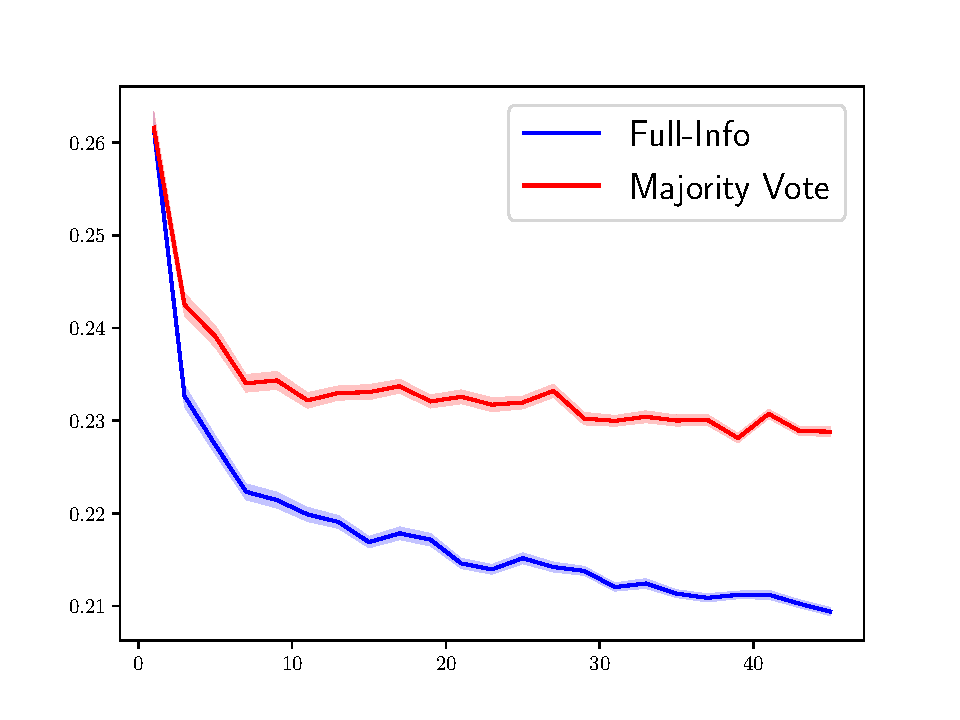
\includegraphics[width=0.45\textwidth]{figure/resnet-class-new.pdf}
			%		& 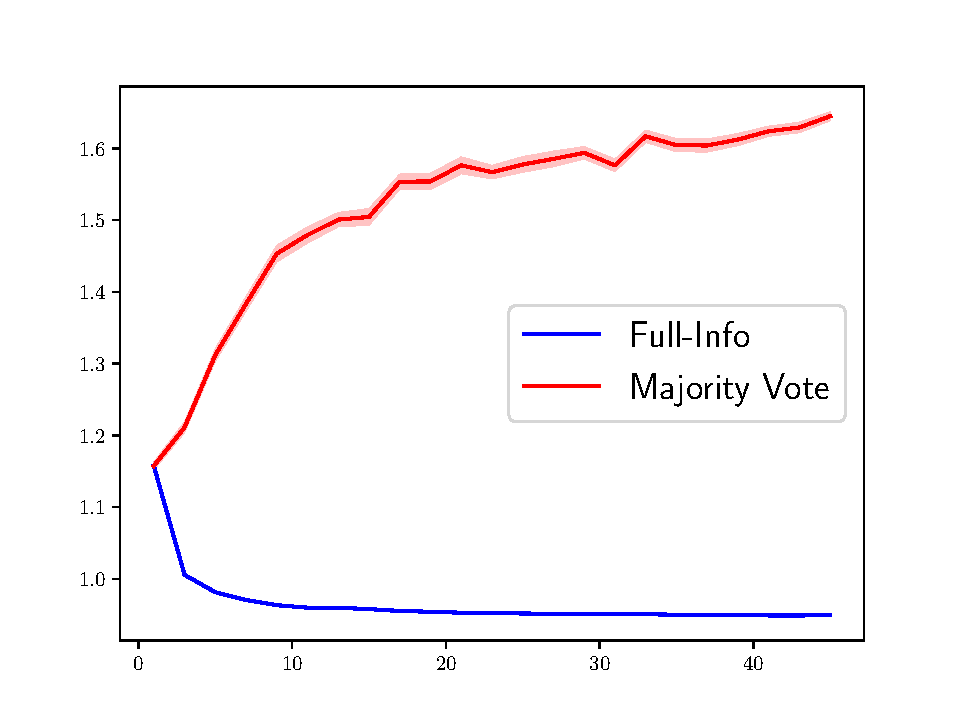
\includegraphics[width=0.45\textwidth]{figure/resnet-calib-new.pdf} \\
			%		(a) & (b) 
			%	\end{tabular}
		%	\caption{Experiments on CIFAR-10H dataset with (a) classification error and (b) calibration error with ResNet features when $d=40$. The classification error is the $0$-$1$ error compared to true labels. The calibration error is measured by $|\mathsf{logit}(\tilde{p}_i) - \mathsf{logit}(\hat{p}_i)|$ where $\tilde{p}_i$ is the predicted probability and $\hat{p}_i$ is the empirical probability. The errors are measured by ten-fold cross-validation. For each fixed $m$, we create $m$ labels for each image by subsampling and average over 100 trials. The error bars show 95\% confidence bands.} \label{fig:cifar}
		%\end{figure}
\input{lower-bound-supp.tex}
\section{Technical lemmas} \label{sec:technical}

We collect several technical lemmas and their proofs in this section, which
will be helpful in the main proofs. See
Appendices~\ref{proof:Sigma-inverse}, \ref{proof:t-Z-integral-noise},
\ref{proof:m-rho-integral-noise-general} and
\ref{proof:rademacher-symmetrization} for their proofs.

\begin{lemma} \label{lem:Sigma-inverse}
  Suppose $A, B \in \mathbb{R}^{d \times d}$ are symmetric, $AB = BA = 0$
  and the matrix $A+B$ is invertible. Then
  \begin{align*}
    \left(A +B\right)^{-1} = A^\dagger + B^\dagger.
  \end{align*}
\end{lemma}

The next two lemmas characterize asymptotic behaviors of expectations
involving a fixed function $f$ and some random variable $Z$ that satisfies
Assumption~\ref{assumption:z-density} for given $\beta>0$ and $c_Z <
\infty$. To facilitate stating the theorems, we recall
that such $Z$ are $(\beta,
c_Z)$-regular.
\begin{lemma} \label{lem:t-Z-integral-noise}
  Let $\beta > 0$ and $f$ be a function on $\R_+$ such that
  $z^{\beta-1}f(z)$ is integrable. If $Z$ is $(\beta,
  c_Z)$-regular (Assumption~\ref{assumption:z-density}), then
  \begin{align*}
    \lim_{t \to \infty} t^\beta \Ep [f(t|Z|)] =  c_Z \int_{0}^{\infty} z^{\beta - 1} f(z) dz.
  \end{align*}
\end{lemma}

\begin{lemma} \label{lem:m-rho-integral-noise-general}
  Let $\beta > 0$ and $c_Z < \infty$, and $Z$ be $(\beta, c_Z)$-regular, let
  $f : \R_+ \to \R$ satisfy $|f(z)| \leq a_0 + a_p z^p$ for some $a_0, a_p <
  \infty$ and all $z \in \R$, and assume $|Z|$ has finite $p$th
  moment. Additionally let $\rho_m(t)$ be the majority vote prediction
  function~\eqref{eq:link-function-m-majority-vote-general} and
  Assumption~\ref{assumption:condition-misspcfd-link-majority-vote} hold for
  each $\sigma_j\opt$ with limiting average derivative
  ${\wb{\sigma}\opt}'(0)$ at zero. Then for any $c > 0$
  \begin{align*}
    \lim_{m \to \infty} m^{\frac{\beta}{2}}\Ep \left[f(\sqrt{m}|Z|) (1 - \rho_m(cZ))\right] = c_Z \int_0^\infty z^{\beta - 1} f(z) \Phi \left(-2 {\wb{\sigma}\opt}'(0) cz\right) dz,
  \end{align*}
  where $\Phi(z) = \int_{-\infty}^z \frac{1}{\sqrt{2 \pi}}
  e^{-\frac{t^2}{2}}dt$ is the standard normal cumulative distribution function.
\end{lemma}

The fourth lemma is a uniform convergence result for the empirical risk in
the case that we have potentially distinct link functions
(cf.~Sec.~\ref{sec:master-results-sem}).
\begin{lemma}
  \label{lemma:rademacher-symmetrization}
  Assume $\E[\ltwo{X}^{\gamma}] \le M^\gamma$ for some $M \ge 1$ and $\gamma
  \ge 2$ and let the radius $1 \le r < \infty$. Let $\Flink \subset \{\sigma
  : \R \to [0, 1], \lipnorm{\sigma} \le \lipconst\}$.  Then for a constant
  $C \lesssim \sqrt{d \lipconst}$, we have
  \begin{equation*}
    \E\left[\sup_{\ltwo{\theta} \le r}
      \sup_{\vec{\sigma} \in \Flink^m} |P_n \loss_{\vec{\sigma},\theta} - L(\theta,
      \vec{\sigma})|\right]
    \le C \cdot
    (M r)^\frac{4\gamma}{3\gamma + 1} 
    \left(\frac{m}{n}\right)^\frac{\gamma}{3\gamma + 1}
    \sqrt{\log(rn)}.
  \end{equation*}
\end{lemma}


\subsection{Proof of Lemma~\ref{lem:Sigma-inverse}}
\label{proof:Sigma-inverse}

As $AB=BA=0$, the symmetric matrices $A$ and $B$ commute and so are
simultaneously orthogonally diagonalizable~\cite[Thm.~4.5.15]{HornJo85}. As
$AB=BA=0$, we can thus write
\begin{align*}
	A = U \begin{bmatrix} \Lambda_1 & 0 \\ 0 & 0 \end{bmatrix} U^\top  , \qquad B = U \begin{bmatrix} 0 & 0 \\ 0 & \Lambda_2 \end{bmatrix} U^\top  ,
\end{align*}
for some orthogonal $U \in \R^{d \times d}$, and as $A+B$ is invertible,  $\Lambda_1, \Lambda_2$ are invertible diagonal matrices. We conclude the proof by writing
\begin{align*}
	(A+ B)^{-1} = U \begin{bmatrix} \Lambda_1^{-1} & 0 \\ 0 & \Lambda_2^{-1} \end{bmatrix} U^\top = U \begin{bmatrix} \Lambda_1^{-1} & 0 \\ 0 & 0 \end{bmatrix} U^\top + U \begin{bmatrix} 0 & 0 \\ 0 & \Lambda_2^{-1} \end{bmatrix} U^\top = A^\dagger + B^\dagger .
\end{align*}

\subsection{Proof of Lemma~\ref{lem:t-Z-integral-noise}}  \label{proof:t-Z-integral-noise}
By the change of variables $w =t z$, we have
\begin{align*}
	t^\beta \Ep [f(t|Z|)] & = \int_{0}^{\infty} f(t z) \cdot t^{\beta - 1} p(z)  \cdot td z =  \int_{0}^{\infty} f(w) \cdot t^{\beta-1} p (w/t) d w \\
	& =  \int_{0}^{\infty} w^{\beta - 1} f(w) \cdot (w/t)^{1-\beta} p (w/t) d w.
\end{align*}
As $|  w^{\beta - 1} f(w) \cdot (w/t)^{1-\beta} p (w/t)| \leq \sup_{z \in (0, \infty)} z^{1-\beta} p(z) \cdot |w^{\beta - 1} f(w)|$, where $w^{\beta - 1} f(w)$ is integrable by assumption, we can invoke dominated convergence to see that
\begin{align*}
	\lim_{t \to \infty} t^\beta \Ep [f(t|Z|)] = \int_{0}^{\infty} w^{\beta - 1} f(w) \cdot \lim_{t \to \infty} (w/t)^{1-\beta} p (w/t) d w = c_Z \int_{0}^{\infty} w^{\beta - 1} f(w) dw.
\end{align*}

\subsection{Proof of Lemma~\ref{lem:m-rho-integral-noise-general}} \label{proof:m-rho-integral-noise-general}
By rescaling arguments, it suffices to prove the theorem for any function
$f$ satisfying
$|f(z)| \leq 1 + z^p$ on $\R_+$ for any $p \in \N$ such that $|Z|$
has finite $p$th moment.  For such $f$, we wish to
show
\begin{align*}
  \lim_{m \to \infty} m^{\frac{\beta}{2}} \Ep \left[f(\sqrt{m}|Z|) (1 - \rho_m(c Z))\right] = c_Z \int_0^\infty z^{\beta-1} f(z) \Phi \left(-2 {\wb{\sigma}\opt}'(0) c z\right) dz,
\end{align*}
where $\Phi$ is the standard normal cdf. The key insight is that we can
approximate $1 - \rho_m(t)$ by a suitable Gaussian cumulative distribution
function (recognizing that $\rho_m(t) > \half$ for $t \neq 0$ by
definition~\eqref{eq:link-function-m-majority-vote-general} as the
probability the majority vote is correct given margin
$\<\theta\opt, X\> = t$).

We first assume $Z \geq 0$ with probability $1$, as the general result
follows by writing $Z = (Z)_+ - (-Z)_+$.  We decompose into two
expectations, depending on $Z$ being large or small:
\begin{align}
  \lefteqn{m^{\frac{\beta}{2}} \Ep \left[f(\sqrt m |Z|) (1 - \rho_m(cZ)) \right]}
  \nonumber \\
  & = \underbrace{m^{\frac{\beta}{2}} \Ep \left[f(\sqrt m Z) (1 - \rho_m(cZ)) \ind\left\{0 \leq Z \leq \frac{M}{\sqrt m}\right\} \right]}_{\mathrm{(I)}} + \underbrace{m^{\frac{\beta}{2}} \Ep \left[f(\sqrt m Z) (1 - \rho_m(cZ)) \ind\left\{Z > \frac{M}{\sqrt m}\right\} \right]}_{\mathrm{(II)}}   .  \label{eq:normal-mid-main}
\end{align}
The proof consists of three main parts. 
\begin{enumerate}[leftmargin=2em,label=\arabic*.]
\item We approximate $1-\rho_m(t)$ by a Gaussian cdf.
\item We can approximate term (I) by replacing $1-\rho_m(t)$ with
  the Gaussian cdf, showing that
  \begin{align}
    \left|\lim_{m \to \infty} \mathrm{(I)} - c_Z \int_0^\infty z^{\beta - 1} f(z) \Phi \left( - 2{\wb{\sigma}\opt}'(0) cz \right) dz \right| = o_M(1)   . \label{eq:normal-mid-3}
  \end{align} 
\item For term (II), we show $1- \rho_m(cz)$ is small when $Z > M/\sqrt{m}$, which allows us to show that
  \begin{equation*}
    \limsup_{m \to \infty}
    \left|\mathrm{(II)} \right| = o_M(1).
  \end{equation*}
\end{enumerate} 
Thus by adding the two preceding displays and taking $M \to \infty$, we
obtain the lemma.

\newcommand{\linkstd}{\sigma_m^{\textup{std}}}

Before we dive into further details, we use the shorthand functions
\begin{equation}
  \linkstd(z)
  \defeq, \frac{\sum_{j=1}^m \prns{\sigma_j\opt(cz) - \half}}{\sqrt{\sum_{j=1}^m \sigma_j\opt(cz)\prns{1 - \sigma_j\opt(cz)}}},
  ~~~
  \Delta_m(z) \defeq 1 - \rho_m(cz) - \Phi(- \linkstd(z))
  \label{eqn:std-link},
\end{equation}
and we also write $p_\infty(\beta) := \sup_{z \in (0, \infty)} z^{1-\beta}
p(z) < \infty$.

\paragraph{Part 1. Normal approximation for $1- \rho_m(t)$ when $t = O(1/\sqrt{m})$.} Let $p_j = \sigma_j\opt(t)$ for shorthand and $Y_j \sim \mathrm{Bernoulli}(p_j)$ be independent random variables. For $t > 0$, then
\begin{align*}
  1 - \rho_m(t) & = \Prb \prn{Y_1 + \cdots + Y_m < \half} = \Prb
  \prn{\frac{\sum_{j=1}^m (Y_j - p_j)}{\sqrt{\sum_{j=1}^m p_j
        (1-p_j)}} < - \frac{\sum_{j=1}^m (p_j - \half)}{
      \sqrt{\sum_{j=1}^m p_j (1-p_j)}}} .
\end{align*}
Consider the centered and standardized random variables $\xi_j = (Y_j - p_j)/\sqrt{\sum_{j=1}^m p_j (1-p_j)} $ so that $\xi_1, \dots, \xi_m$ are zero mean, mutually independent, and satisfy
\begin{align*}
  \sum_{j=1}^m \var \prn{\xi_j} & = 1  , \\
  \sum_{j=1}^m \Ep \brk{\left|\xi_j\right|^3} & =
  \frac{\sum_{j=1}^m p_j (1-p_j)(p_j^2 + (1-p_j)^2)}{\prns{\sum_{j=1}^m p_j (1-p_j)}^{3/2}}
  \leq \frac{\max_{1 \leq j \leq m} (p_j^2 + (1-p_j)^2)}{\sqrt{\sum_{j=1}^m p_j(1-p_j)}}  .
\end{align*} 
By the Berry-Esseen theorem (cf.~\citet{ChenGoSh10, Shevtsova14}), for all
$t > 0$
\begin{align*}
	\left|1 - \rho_m(t) - \Phi \left(-\frac{ \sum_{j=1}^m \left( p_j - \half\right)}{\sqrt{\sum_{j=1}^m p_j (1-p_j)}}\right)\right| \leq \frac{3}{4} \cdot \frac{\max_{1 \leq j \leq m} (p_j^2 + (1-p_j)^2)}{\sqrt{\sum_{j=1}^m p_j (1-p_j)}}  .
\end{align*}
%
Fix any $M <\infty$. Then for $0 \leq t \leq cM /\sqrt m$ and large enough
$m$, the right hand side of the preceding display has the upper bound
$2/\sqrt{m}$, as in numerator we have $p_j^2 + (1-p_j)^2 \leq 1$, and in
denominator $\min_{1 \leq j \leq m}p_j(1-p_j) \to 1/4$ for all $j$ as $m \to
\infty$, which follows from
Assumption~\ref{assumption:condition-misspcfd-link-majority-vote}
that
\begin{equation*}
  \half \leq \limsup_{m \to \infty} \max_{1 \leq j \leq m} p_j \leq \limsup_{m \to \infty} \sup_{1 \leq j < \infty} {\sigma_j\opt} \prn{\frac{cM}{\sqrt m} } =
  \half.
\end{equation*}
By repeating the same argument for $-cM /\sqrt m \leq t < 0$, we obtain that for large $m$ and $|t| \leq cM / \sqrt m$,
\begin{align}
  \left|1 - \rho_m(t) - \Phi \left(-\left|\frac{ \sum_{j=1}^m \left( \sigma_j\opt(t) - \half\right)}{\sqrt{\sum_{j=1}^m \sigma_j\opt(t) \prn{1 - \sigma_j\opt(t)}}}\right|\right)\right| \leq \frac{2}{\sqrt m}   . \label{eq:BE-approximation}
\end{align}

\paragraph{Part 2. Approximating (I) by Gaussian cdf.}
For the first term (I) in~\eqref{eq:normal-mid-main}, we further decompose into a normal approximation term and an error term,
\begin{align*}
  \mathrm{(I)} = \underbrace{m^{\frac{\beta}{2}}
    \Ep \left[f(\sqrt m Z)\Phi(-\linkstd(z))
      \ind\left\{0 \leq Z \leq \frac{M}{\sqrt m}\right\} \right]}_{\mathrm{(III)}} + \underbrace{m^{\frac{\beta}{2}} \Ep \left[f(\sqrt m Z)\Delta_m(z) \ind\left\{0 \leq Z \leq \frac{M}{\sqrt m}\right\} \right]}_{\mathrm{(IV)}}, %\label{eq:normal-mid-0}
\end{align*}
where $\Delta_m(z) = 1 - \rho_m(cz) - \Phi(-\linkstd(z))$ as in
def.~\eqref{eqn:std-link}. We will show $\mathrm{(IV)} \to 0$ and so
$\mathrm{(III)}$ dominates. By the change of variables $w = \sqrt{m}z$, we can
further write (III) as
\begin{align*}
  \mathrm{(III)} 
  & = m^{\frac{\beta}{2}} \int_0^{\frac{M}{\sqrt m}} f(\sqrt m z) \Phi
  ( -\linkstd(z)) \cdot p(z) d z \nonumber \\
  & = \int_0^{M} w^{\beta - 1} f(w) \Phi  \left( - \linkstd\prn{\frac{w}{\sqrt m}}\right) \cdot  (w/\sqrt{m})^{1-\beta} p(w/\sqrt{m}) d w   .
\end{align*}
We want to take the limit $m \to \infty$ and apply dominated convergence
theorem. Because $(w/\sqrt{m})^{1-\beta} p(w/\sqrt{m}) \leq p_\infty(\beta)
< \infty$ and $\linkstd(w/\sqrt m) \geq 0$, we have
\begin{align*}
	&  w^{\beta - 1} f(w) \Phi  \left( - \linkstd\prn{\frac{w}{\sqrt m}}\right) \cdot  \left( - \linkstd\prn{\frac{w}{\sqrt m}}\right) \cdot  (w/\sqrt{m})^{1-\beta} p(w/\sqrt{m}) \leq w^{\beta - 1} f(w) \cdot \Phi(0) p_\infty(\beta)   .
\end{align*} 
As $\beta > 0$ and $|f(w)| \leq 1 + w^p$, $w^{\beta - 1} f(w)$ is integrable
on $[0, M]$, and by~\eqref{ass:misspcfd-link-1} and \eqref{ass:misspcfd-link-3}
  in Assumption~\ref{assumption:condition-misspcfd-link-majority-vote},
\begin{align*}
	\lim_{m \to \infty} \linkstd\prn{\frac{w}{\sqrt m}} & = \lim_{m \to \infty}\frac{\sqrt{m}\left(\wb{\sigma}_m\opt\prn{\frac{cw}{\sqrt m}}-\frac{1}{2}\right)}{\sqrt{ \frac{1}{m} \sum_{j=1}^m \sigma_j\opt\prn{\frac{cw}{\sqrt m}}\prn{1 - \sigma_j\opt\prn{\frac{cw}{\sqrt m}}}}} =  2 {\wb{\sigma}\opt}'(0) cw   .
\end{align*}
Using the above display and that $\lim_{m \to \infty} (w/\sqrt{m})^{1-\beta}
p(w/\sqrt{m}) = c_Z$, we can thus apply dominated convergence theorem
to conclude that
\begin{align*}
	\lim_{m \to \infty}\mathrm{(III)} 
%	&  = \int_0^{M} w^{\beta - 1} f(w) \cdot   \Phi  \left( -\lim_{m \to \infty} \linkstd(z)\right) \cdot \lim_{m \to \infty} w^{\beta - 1}m^{\frac{\beta - 1}{2}} p(wm^{-\frac{1}{2}}) d w \nonumber \\
	&  = c_Z \int_0^M w^{\beta - 1} f(w) \cdot  \Phi  \left( - 2 {\wb{\sigma}\opt}'(0) cw\right) dw = c_Z \int_0^\infty w^{\beta - 1} f(w) \Phi \left( - 2{\wb{\sigma}\opt}'(0) cw \right) dw + o_M(1). %\label{eq:normal-mid-1}
\end{align*} 

Next we turn to the error term (IV). By the
bound~\eqref{eq:BE-approximation}, $|\Delta_m(z)| \leq 2/\sqrt{m}$ when $|z|
\leq M/\sqrt{m}$ for large enough $m$, and substituting $w = \sqrt{m}z$,
\begin{align*}
	|\mathrm{(IV)}| & \leq m^{\frac{\beta}{2}} \Ep \left[|f(\sqrt m Z)| \cdot \frac{2}{\sqrt m} \cdot \ind\left\{0 \leq Z \leq \frac{M}{\sqrt m}\right\}   \right] \nonumber \\
	& = \frac{2}{\sqrt m} \int_0^{\frac{M}{\sqrt m}} \sqrt m \cdot |f(\sqrt m z)| \cdot m^{\frac{\beta-1}{2}} p(z) dz  = \frac{2}{\sqrt m} \int_0^M w^{\beta - 1}|f(w)| \cdot(w/\sqrt{m})^{1-\beta} p(w/\sqrt{m}) dw.
\end{align*}
By using Assumption~\ref{assumption:z-density} again that $(w/\sqrt{m})^{1-\beta} p(w/\sqrt{m}) \leq p_\infty(\beta) < \infty$, we further have
\begin{equation*}
  |\mathrm{(IV)}| 
  \leq \frac{2p_\infty(\beta) }{\sqrt m} \cdot \int_0^M w^{\beta - 1}|f(w)| dw
  \leq  \frac{2p_\infty(\beta) }{\sqrt m} \cdot
  \prn{\frac{M^\beta}{\beta} +\frac{M^{p+\beta}}{p+\beta}}
  \to 0,
\end{equation*}
where we use $|f(w)| \leq 1+w^p$. We have thus shown the
limit~\eqref{eq:normal-mid-3}.

%Substitute Eqs.~\eqref{eq:normal-mid-1} and \eqref{eq:normal-mid-2} into Eq.~\eqref{eq:normal-mid-0}, we obtain
%\begin{align*}
%	\left|\lim_{m \to \infty} \mathrm{(I)} - c_Z \int_0^\infty w^{\beta - 1} f(w) \Phi \left( - 2{\wb{\sigma}\opt}'(0) cw \right) dw \right| = o_M(1)   .
%\end{align*} 
\paragraph{Part 3. Upper bounding (II).}
In term~(II), when $Z$ is large, the key is that the quantity
$1-\rho_m(t)$ is
small when $|t| \geq cM /\sqrt{m}$: Hoeffding's
inequality implies the tail bound
\begin{align*}
  0 \leq 1 - \rho_m(t) \leq e^{-2 \left(\wb{\sigma}_m\opt(t) - \half\right)^2 m}  .
\end{align*}
Thus
\begin{align}
	|\mathrm{(II)}| &\leq  \int_{\frac{M}{\sqrt m}}^1 \sqrt m |f(\sqrt m z)|  e^{-2\left(\wb{\sigma}_m\opt(cz) - \half\right)^2m}\cdot  m^{\frac{\beta-1}{2}} p(z) dz + \int_{1}^\infty m^{\frac \beta 2} |f(\sqrt m z)|  e^{-2\left(\wb{\sigma}_m\opt(cz) - \half\right)^2m}\cdot  p(z) dz   . \nonumber  
\end{align}
Using the assumption that $\gamma \defeq\liminf_m \inf_{t \geq c}
\prn{\wb{\sigma}_m\opt(t) - \half} > 0$ from~\eqref{ass:misspcfd-link-2},
that $|f(z)| \leq 1 +z^p$ and $|Z|$ has finite $p$th moment, we observe
that
\begin{align*}
	\int_{1}^\infty m^{\frac \beta 2} |f(\sqrt m z)|  e^{-2\left(\wb{\sigma}_m\opt(cz) - \half\right)^2m}\cdot  p(z) dz\leq  m^{\frac{1}{2}(\beta + p)}  e^{-2\gamma^2m} \int_1^\infty (1 + z^p) p(z) dz \to 0  ,
\end{align*}
and consequently
\begin{align*} 
	\limsup_{m \to \infty} |\mathrm{(II)}|  & \leq  \limsup_{m \to \infty} \int_{\frac{M}{\sqrt m}}^1 \sqrt m |f(\sqrt m z)|  e^{-2\left(\wb{\sigma}_m\opt(cz) - \half\right)^2m}\cdot  m^{\frac{\beta-1}{2}} p(z) dz \nonumber \\
	& = \limsup_{m \to \infty}   \int_{M}^{\sqrt{m}}  w^{\beta - 1} |f(w)| e^{-2\left(\wb{\sigma}_m\opt\prn{\frac{cw}{\sqrt m}} - \half\right)^2m} \cdot (w/\sqrt{m})^{1-\beta} p(w/\sqrt{m}) d w   .
\end{align*}
For $w \in [M, \sqrt m]$, we have
\begin{align*}
	\left(\wb{\sigma}_m\opt\prn{\frac{cw}{\sqrt m}} - \half\right)^2m & = \left(\frac{\wb{\sigma}_m\opt\prn{\frac{cw}{\sqrt m}} - \half}{\frac{cw}{\sqrt m}}\right)^2 c^2 w^2 \geq \left(\inf_{0 < t \leq c} \frac{\wb{\sigma}_m\opt(t) - \half}{t}\right)^2 c^2 w^2   ,
\end{align*}
while Assumption~\eqref{ass:misspcfd-link-2} gives $\delta:=\inf_{0 < t \leq c} \frac{\wb{\sigma}_m\opt(t) - \half}{t} > 0$,  so
\begin{align*}
\limsup_{m \to \infty} |\mathrm{(II)}| & \leq \int_{M}^{\sqrt{m}}  w^{\beta - 1} |f(w)| e^{-\delta w^2} \cdot (w/\sqrt{m})^{1-\beta} p(w/\sqrt{m}) d w. %\label{eq:normal-mid-4}
\end{align*}
Using the inequality
$(w/\sqrt{m})^{1-\beta} p(w/\sqrt{m}) \leq p_\infty(\beta) < \infty$, we
apply dominated convergence:
\begin{align*}
  \lim_{m \to \infty} \int_{M}^{\sqrt{m}}  w^{\beta - 1} |f(w)| e^{-\delta w^2} \cdot (w/\sqrt{m})^{1-\beta} p(w/\sqrt{m}) d w  = c_Z \int_M^\infty  w^{\beta - 1}  |f(w)| e^{-\delta w^2} dw = o_M(1).
\end{align*}

\subsection{Proof of Lemma~\ref{lemma:rademacher-symmetrization}} \label{proof:rademacher-symmetrization}
We follow a typical symmetrization approach, then construct a covering
that we use to prove the lemma.
Let $P_n^0 = n^{-1} \sum_{i = 1}^n \varepsilon_i 1_{X_i, Y_i}$ be the
(random) symmetrized measure with point masses at $(X_i, Y_i)$ for
$Y_i = (Y_{i1}, \ldots, Y_{im})$. Then by a standard symmetrization
argument, we have
\begin{equation}
	\label{eqn:symmetrization-step}
	\E\left[\sup_{\ltwo{\theta} \le r}
	\sup_{\vec{\sigma} \in \Flink^m} |P_n \loss_{\vec{\sigma},\theta} - L(\theta,
	\vec{\sigma})|\right]
	\le 2 \E\left[\sup_{\ltwo{\theta} \le r}
	\sup_{\vec{\sigma} \in \Flink^m} \left|P_n^0 \loss_{\vec{\sigma}, \theta}
	\right|\right].
\end{equation}

We use a covering argument to bound the symmetrized
expectation~\eqref{eqn:symmetrization-step}.  Let $R < \infty$ to be
chosen, and for an (again, to be determined) $\epsilon > 0$ let $\mc{G}
\subset \Flink$
denote an $\epsilon$-cover of $\Flink$ in the supremum norm on $[-R, R]$,
that is, $\norm{g - \sigma} = \sup_{t \in [-R,R]} |g(t) - \sigma(t)|$, and
so for each $\sigma \in \Flink$ there exists $g \in \mc{G}$ such that
$\norm{g - \sigma} \le \epsilon$. Then~\cite[Ch.~2.7]{VanDerVaartWe96} we
have $\log \card(\mc{G}) \le O(1) \frac{R \lipconst}{\epsilon}$. Let
$\Theta_\epsilon$ be a minimal $\epsilon$-cover of $\{\theta \mid
\ltwo{\theta} \le r\}$ in $\ltwo{\cdot}$, so that $\log
\card(\Theta_\epsilon) \le d \log(1 + \frac{2r}{\epsilon})$
and $\max_{\theta \in \Theta_\epsilon} \ltwo{\theta} \le r$.
We claim that for each $\ltwo{\theta} \le r$ and $\sigma
\in \Flink$, there exists
$v \in \Theta_\epsilon$ and $g \in \mc{G}$ such that
\begin{equation}
	\left|\frac{1}{n} \sum_{i = 1}^n \varepsilon_i
	\left(\loss_{\sigma, \theta}(Y_{ij} \mid X_i)
	-
	\loss_{g, v}(Y_{ij} \mid X_i)\right)
	\right|
	\le \epsilon +
	\frac{1}{n}\sum_{i = 1}^n \ltwo{X_i} \epsilon
	+ \frac{1}{n} \sum_{i = 1}^n\indic{\ltwo{X_i} \ge R / r}.
	\label{eqn:covering-diff}
\end{equation}
Indeed, for any $g \in \Flink$ and $\theta, v \in \R^d$, we have
\begin{align*}
	\left|\loss_{\sigma, \theta}(y \mid x)
	- \loss_{g, v}(y \mid x)\right|
	& = \left|\int_0^{y \<x, \theta\>} \sigma(-t) dt
	- \int_0^{y \<x, v\>} g(-t) dt\right| \\
	& \le \sup_{|t| \le r \ltwo{x}} |\sigma(t) - g(t)|
	+ \left|\int_{y\<x, v\>}^{y\<x, \theta\>}
	|\sigma(-t) - g(-t)| dt \right| \\
	& \le \norm{\sigma - g} + \indic{\ltwo{x} \ge R/r}
	+ |\<x, \theta - v\>| \\
	& \le
	\norm{\sigma - g} + \ltwo{x} \ltwo{\theta - v}
	+ \indic{\ltwo{x} \ge R/r},
\end{align*}
where we have used that $\sigma, g \in [0, 1]$.
Taking the elements $g, v$ in the respective coverings to minimize
the above bound gives the guarantee~\eqref{eqn:covering-diff}.

We now leverage inequality~\eqref{eqn:covering-diff}
in the symmetrization step~\eqref{eqn:symmetrization-step}.
We have
\begin{align*}
	\lefteqn{\E\left[\sup_{\ltwo{\theta} \le r}
		\sup_{\vec{\sigma} \in \Flink^m} |P_n \loss_{\vec{\sigma},\theta} - L(\theta,
		\vec{\sigma})|\right]} \\
	& \lesssim
	\E\left[\max_{\theta \in \Theta_\epsilon}
	\max_{\vec{g} \in \mc{G}^m}
	\left|P_n^0 \loss_{\vec{g}, \theta}\right|
	\right]
	+ \epsilon + \E[\ltwo{X_1}] \epsilon
	+ \frac{1}{n} \sum_{i = 1}^n \P(\ltwo{X_i} \ge R / r) \\
	& \stackrel{(i)}{\lesssim}
	\sqrt{\frac{d m R \lipconst}{\epsilon}
		\log\left(1 + \frac{2r}{\epsilon}\right)}
	\E\left[\frac{r^2}{n}\sum_{i = 1}^n \ltwo{X_i}^2\right]^{1/2}
	+ \epsilon + \E[\ltwo{X_1}] \epsilon
	+ \frac{\E[\ltwo{X_i}^{\gamma}]}{(R/r)^{\gamma}} \\
	& \le
	M r \sqrt{\frac{dm R \lipconst}{n \epsilon}
		\log \left(1 + \frac{2r}{\epsilon}\right)}
	+ (M + 1) \epsilon
	+ \frac{M^{\gamma}}{(R/r)^{\gamma}},
\end{align*}
where inequality $(i)$ uses that if $Z_i$ are $\tau^2$-sub-Gaussian, then
$\E[\max_{i \le N} |Z_i|] \le \sqrt{2 \tau^2 \log N}$, and that
conditional on $\{X_i, Y_i\}_{i = 1}^n$, the symmetrized sum $\sum_{i =
	1}^n \varepsilon_i \frac{1}{m} \sum_{j = 1}^m \loss_{g_j, \theta}(Y_{ij}
\mid X_i)$ is $r^2 \sum_{i = 1}^n \ltwo{X_i}^2$-sub-Gaussian, as
$|\loss_{g_j, \theta}(Y_{ij} \mid X_i)| \le |\<X_i, \theta\>| \le r
\ltwo{X_i}$.  We optimize this bound to get the final guarantee of the
lemma: set $\epsilon = (Rm / n)^{1/3}$ (and note that we will
choose $R \ge 1$) to obtain
\begin{equation*}
	\E\left[\sup_{\ltwo{\theta} \le r}
	\sup_{\vec{\sigma} \in \Flink^m} |P_n \loss_{\vec{\sigma},\theta} - L(\theta,
	\vec{\sigma})|\right]
	\lesssim \sqrt{d \lipconst \log(rn)}
	M r \left(\frac{R m}{n}\right)^{1/3}
	+ \frac{(Mr)^\gamma}{R^\gamma}.
\end{equation*}
Choose $R
= ((Mr)^{3(\gamma - 1)} n / m)^\frac{1}{3\gamma + 1}$.

%\subsection{Proof of Lemma~\ref{lemma:glivenko-cantelli}} \label{proof:glivenko-cantelli}
%We use a more or less standard Rademacher complexity and
%symmetrization argument. Let
%$\Prb_{n}'$ denote an independent copy of $\Prb_{n}$, that is, we draw
%independent copies $X_i'$ and, draw $Y_{ij}'$
%independently conditional on $X_i'$ according to the same distribution from which $Y_{ij} \mid X_i$ are drawn. Let $\varepsilon_i \in \{\pm 1\}$ be
%i.i.d.\ uniform signs. Then for any $1 \le k < \infty$,
%\begin{align*}
%	\Ep\left[\sup_{\ltwo{\theta} \le r, \eta \in \mathcal{E}} \left|\Prb_n\loss_{\theta, \eta} -
%	\Prb \loss_{\theta, \eta} \right|^k\right]
%	& \le \Ep\left[\sup_{\ltwo{\theta} \le r, \eta \in \mathcal{E}}
%	\left|(\Prb_{n} - \Prb_{n}') \loss_{\theta, \eta} \right|^k\right] \\
%	& \le 2^k \Ep\left[\sup_{\ltwo{\theta} \le r, \eta \in \mathcal{E}}
%	\left|\frac{1}{n} \sum_{i = 1}^n \varepsilon_i
%	\left(\frac{1}{m} \sum_{j = 1}^m \prn{h_{\eta, j}(Y_{ij} \<\theta, X_i\>)
%		- h_{\eta, j}(0) }\right)\right|^k\right],
%\end{align*}
%where the first inequality is Jensen's and the second adds and subtracts
%$\frac{1}{m} \sum_{j=1}^m h_{\eta, j}(0) = \loss_{0,\eta}$, then uses that $\frac{1}{m} \sum_{j = 1}^m h_{\eta, j}(Y_{ij} \<\theta, X_i\>) - \frac{1}{m} \sum_{j = 1}^m h_{\eta, j}(Y_{ij}' \<\theta, X_i'\>)$ is
%symmetric. Next apply Jensen's inequality once again for $|x|^k$ we have
%\begin{align*}
%	\Ep\left[\sup_{\ltwo{\theta} \le r, \eta \in \mathcal{E}} \left|\Prb_n\loss_{\theta, \eta} -
%	\Prb \loss_{\theta, \eta} \right|^k\right] \leq \frac{2^k}{m} \sum_{j=1}^m \Ep\left[\sup_{\ltwo{\theta} \le r, \eta \in \mathcal{E}}
%	\left|\frac{1}{n} \sum_{i = 1}^n \varepsilon_i
%	\left(\prn{h_{\eta, j}(Y_{ij} \<\theta, X_i\>)
%		- h_{\eta, j}(0) }\right)\right|^k\right]
%\end{align*}
%Applying the Rademacher contraction
%inequality~\cite[Thm.~4.12]{LedouxTa91},
%we thus obtain
%\begin{align*}
%	\Ep\left[\sup_{\ltwo{\theta} \le r, \eta \in \mathcal{E}} \left|\Prb_n\loss_{\theta, \eta} -
%	\Prb \loss_{\theta, \eta} \right|^k\right]
%	& \le \frac{4^k}{m} \sum_{j=1}^m \Ep\left[\sup_{\ltwo{\theta} \le r}
%	\left|\frac{1}{n} \sum_{i = 1}^n \varepsilon_i
%	\cdot \mathsf{L} Y_{ij} \<\theta, X_i\>\right|^k\right] \\
%	& = \frac{\prn{4\mathsf{L}r}^k}{m} \sum_{j=1}^m \Ep\left[
%	\ltwo{\frac 1 n\sum_{i = 1}^n \varepsilon_i X_i  Y_{ij}}^k
%	\right] \\
%	& \le \left(\frac{4 \mathsf{L}r \sqrt{k}}{n}\right)^k
%	\Ep\left[\left(\sum_{i = 1}^n \ltwo{X_i}^2\right)^{k/2}
%	\right],
%\end{align*}
%where the final inequality uses that $Y_{ij} \in \{\pm 1\}$ and standard
%Khintchine-type bounds in Hilbert spaces~\cite[Sec.~1.4]{delaPenaGi99}.
%Finally, we note that $\Ep[(\sum_{i = 1}^n \ltwo{X_i}^2)^{k/2}] \le n^{k/2}
%\frac{1}{n} \sum_{i = 1}^n \Ep[\ltwo{X_i}^{k}]$ for all $k \ge 2$ by
%Jensen's inequality. Applying
%Markov's inequality, for any $t \ge 0$ and $k \ge 1$,
%\begin{align*}
%	\Prb\left(\sup_{\ltwo{\theta} \le r}
%	\left|\Prb_{n,m}\loss_\theta - \poploss(\theta) \right| \ge t \right)
%	& \le \left(\frac{4 \mathsf{L} r \sqrt{k}}{t \sqrt{n}}\right)^k
%	\Ep[\ltwo{X_1}^k].
%\end{align*}
%For $k > 2$, this is summable, so that the Borel-Cantelli theorem gives
%a.s.\ convergence. Take $n \to \infty$ to get the result.


\section{Proof of Theorem~\ref{theorem:multilabel-asymptotics}}
\label{sec:proof-multilabel-asymptotics}

Let $t_m$ be the solution to $h_{t\opt,m}(t) = 0$ as in
Lemma~\ref{lemma:generic-solutions}. The consistency argument is
immediate: the losses $\loss$ are convex, continuous, and locally Lipschitz,
so~\citet[Thm.~5.4]{ShapiroDeRu09} gives $\what{\theta}_n
\cas \theta\opt_L$. By an appeal to standard
M-estimator theory~\cite[e.g.][Thm.~5.23]{VanDerVaart98},
we thus obtain
\begin{equation}
	\label{eqn:multilabel-basic-asymptote}
	\sqrt{n} \big(\what{\theta}_n - \theta\opt_L\big)
	\cd \normal\left(0, \nabla^2 L(\theta\opt_L, \sigma)^{-1}
	\cov\bigg(\frac{1}{m} \sum_{j = 1}^m
	\nabla \loss_{\sigma,\theta\opt_L}(Y_j \mid X)\bigg)
	\nabla^2 L(\theta\opt_L, \sigma)^{-1} \right).
\end{equation}
We expand the covariance term to obtain the first main result of the
theorem. For shorthand, let $G_j = \nabla \loss_{\sigma,\theta\opt_L}(Y_j
\mid X)$, so that $\sum_{j = 1}^m \E[G_j] = 0$ and the $G_j$ are
conditionally independent given $X$. Applying the law of total covariance,
we have
\begin{align*}
	\cov\bigg(\frac{1}{m} \sum_{j = 1}^m G_j\bigg)
	& = \cov\bigg(\frac{1}{m} \sum_{j = 1}^m
	\E[G_j \mid X]\bigg)
	+ \E\left[\cov\bigg(
	\frac{1}{m} \sum_{j = 1}^m G_j \mid X\bigg)\right] \\
	& =
	\underbrace{\cov\bigg(\frac{1}{m} \sum_{j = 1}^m \E[G_j \mid X] \bigg)}_{
		\mathrm{(I)}}
	+ \frac{1}{m^2} \sum_{j = 1}^m
	\underbrace{\E\left[\cov(G_j \mid X)\right]}_{\mathrm{(II)}},
\end{align*}
where we have used the conditional independence of the $Y_j$ conditional on
$X$.  We control each of terms (I) and (II) in turn.

For the first, we have by the independent decomposition
$X = Z u\opt + \projperp W$ that
\begin{equation*}
	\E[G_j \mid X]
	= 
	\left(\sigma(t_m Z)
	(1 - \sigma_j\opt(t\opt Z))
	- \sigma(- t_m Z) \sigma_j\opt(t\opt Z)\right)
	X,
\end{equation*}
and so
\begin{align*}
	\mathrm{(I)} & =
	\E\left[\left(\sigma(t_m Z) (1 - \wb{\sigma}\opt(t\opt Z))
	- \sigma(-t_m Z) \wb{\sigma}\opt(t\opt Z)\right)^2 XX^\top \right] \\
	& =
	\E\left[\left(\sigma(t_m Z) (1 - \wb{\sigma}\opt(t\opt Z))
	- \sigma(-t_m Z) \wb{\sigma}\opt(t\opt Z)\right)^2 Z^2 \right]
	u\opt {u\opt}^\top
	\\ & \qquad ~ + 
	\E\left[\left(\sigma(t_m Z) (1 - \wb{\sigma}\opt(t\opt Z))
	- \sigma(-t_m Z) \wb{\sigma}\opt(t\opt Z)\right)^2\right]
	\projperp \Sigma \projperp \\
	& = \E[\linkerr(Z)^2 Z^2] u\opt {u\opt}^\top
	+ \E[\linkerr(Z)^2]   \projperp \Sigma \projperp,
\end{align*}
where we used the independence of $W$ and $Z$.
For term (II) above, we see that conditional on $X$,
$\nabla \loss_{\sigma,\theta}(Y_j \mid X)$ is a binary
random variable taking values in
$\{-\sigma(-t_m Z) X, \sigma(t_m Z) X\}$ with probabilities
$\sigma_j\opt(t\opt Z)$ and
$1 - \sigma_j\opt(t\opt Z)$, respectively, so that
a calculation leveraging the variance of Bernoulli random variables
yields
\begin{align*}
	\cov(G_j \mid X)
	& = \sigma_j\opt(t\opt Z) (1 - \sigma_j\opt(t\opt Z))
	\left(\sigma(t_m Z) + \sigma(-t_m Z)\right)^2 XX^\top
	= v_j(Z) XX^\top,
\end{align*}
where we used the definition~\eqref{eqn:error-functions} of the
variance terms.
A similar calculation to that we used for term (I) then gives that
\begin{align*}
	\mathrm{(II)} & = \frac{1}{m^2}
	\sum_{j = 1}^m \E[v_j(Z) Z^2] u\opt {u\opt}^\top
	+ \frac{1}{m^2}
	\sum_{j = 1}^m \E[v_j(Z)] \projperp \Sigma \projperp.
	%% \mathrm{(II)} & =
	%% \frac{1}{m^2} \sum_{j = 1}^m
	%% \E\left[\sigma_j\opt(t\opt Z) (1 - \sigma_j\opt(t\opt Z))
	%%   \left(\sigma(t_m Z) + \sigma(-t_m Z)\right)^2 Z^2 \right] u\opt {u\opt}^\top
	%% \\ & \qquad ~
	%% + \frac{1}{m^2} \sum_{j = 1}^m \E\left[
	%%   \sigma_j\opt(t\opt Z) (1 - \sigma_j\opt(t\opt Z))
	%%   \left(\sigma(t_m Z) + \sigma(-t_m Z)\right)^2\right]
	%% \projperp \Sigma \projperp.
\end{align*}
Applying Lemma~\ref{lem:Sigma-inverse} then allows us to decompose the the
covariance in expression~\eqref{eqn:multilabel-basic-asymptote} into
terms in the span of $u\opt {u\opt}^\top$ and those perpendicular to
it, so that the asymptotic covariance is
\begin{align*}
	\frac{\E[\linkerr(Z)^2 Z^2] + \frac{1}{m^2}
		\sum_{j = 1}^m \E[v_j(Z) Z^2]}{
		\E[\hessfunc(Z) Z^2]^2} u\opt {u\opt}^\top
	+ \frac{\E[\linkerr(Z)^2] + \frac{1}{m^2}
		\sum_{j = 1}^m \E[v_j(Z)]}{\E[\hessfunc(Z)]^2}
	\prn{\projperp \Sigma \projperp}^\dagger,
\end{align*}
by applying Lemma~\ref{lemma:generic-solutions} for the form of the Hessian
$\nabla^2 L(\theta_L\opt, \sigma)$ and Lemma~\ref{lem:Sigma-inverse} for the
inverse, giving the first result of the theorem.

To obtain the second result, we apply the delta method with
the mapping $\phi(x) = x / \ltwo{x}$, which satisfies
$\nabla \phi(x) = (I - \phi(x) \phi(x)^\top) / \ltwo{x}$,
so that for $\what{u}_n = \what{\theta}_n / \ltwos{\what{\theta}_n}$ we have
\begin{align*}
  \sqrt{n}(\what{u}_n - u\opt)
  & \cd
  \normal\left(0, \frac{1}{t_m^2}
  \frac{\E[\linkerr(Z)^2] + \frac{1}{m^2}
    \sum_{j = 1}^m \E[v_j(Z)]}{\E[\hessfunc(Z)]^2}
  \prn{\projperp \Sigma \projperp}^\dagger
  \right)
\end{align*}
as desired.

\subsection{Proof of Lemma~\ref{lemma:generic-solutions}}
\label{sec:proof-generic-solutions}

Recall that $h = h_{t\opt, m}$ is the calibration
gap function~\eqref{eqn:h-m-func}.
We see that because $\E[Z] = 0$, we have
$h(0) = -2 \E[Z \varphi_m(t\opt Z)] < 0$,
while using Assumption~\ref{assumption:model-link} and that
$\E[|Z|] < \infty$, we apply dominated convergence and that
$\lim_{t \to \infty} (\sigma(t Z) - \half) Z = c|Z|$ with probability 1
to obtain
\begin{align*}
	\lim_{t \to \infty} h(t) = \E[c|Z| (1 - \varphi_m(t\opt Z))]
	+ \E[c |Z| \varphi_m(t\opt Z)] = c \E[|Z|] > 0.
\end{align*}
Because $h'(t) = \E[\sigma'(tZ) Z^2 (1 - \varphi_m(t\opt Z))]
+ \E[\sigma'(-tZ) Z^2 \varphi_m(t\opt Z)] > 0$, we see that there
is a unique $t_m$ solving $h(t_m) = 0$, and evidently
$\theta\opt_L = t_m u\opt$ is a minimizer of $L$.

We compute the Hessian of $L$. For this,
we again let $\theta = t u\opt$ to write
\begin{align*}
	\nabla^2 L(\theta, \sigma) & = \E[\sigma'(-\<\theta, X\>) XX^\top \varphi_m(\<X, \theta\opt\>)]
	+ \E[\sigma'(\<\theta, X\>) XX^\top (1 - \varphi_m(\<X, \theta\opt\>))] \\
	& = \E\left[\sigma'(-t Z) \varphi_m(t\opt Z)
	\left(Z^2 u\opt {u\opt}^\top + WW^\top\right)\right]
	+ \E\left[\sigma'(t Z) (1 - \varphi_m(t\opt Z))
	\left(Z^2 u\opt {u\opt}^\top + WW^\top \right)\right] \\
	& = \E\left[\left(\sigma'(-tZ) \varphi_m(t\opt Z)
	+ \sigma'(tZ) (1 - \varphi_m(t\opt Z)) \right) Z^2\right]
	u\opt {u\opt}^\top \\
	& \quad + \E\left[\sigma'(-tZ) \varphi_m(t\opt Z)
	+ \sigma'(tZ) (1 - \varphi_m(t\opt Z))\right] \E[WW^\top],
\end{align*}
which gives $\nabla^2 L(\theta, \sigma) \succ 0$ and so $\theta\opt_L$ is
unique.  Finally, the desired form of the Hessian follows as $\E[WW^\top] =
\projperp \Sigma \projperp$.

\section{Proof of Theorem~\ref{theorem:majority-vote-asymptotics}}
\label{sec:proof-majority-vote-asymptotics}

As in the proof of Theorem~\ref{theorem:multilabel-asymptotics}, we begin
with a consistency result. Let $t_m$ be the solution to $h_{t\opt, m}(t) =
0$ as in Lemma~\ref{lemma:generic-solutions}.
The once again, \citet[Thm.~5.4]{ShapiroDeRu09}
shows that $\what{\theta}_n \cas \theta\opt_L$.
As previously, appealing to standard
M-estimator theory~\cite[e.g.][Thm.~5.23]{VanDerVaart98},
we obtain
\begin{equation}
	\label{eqn:vote-basic-asymptote}
	\sqrt{n} \big(\what{\theta}_n - \theta\opt_L\big)
	\cd \normal\left(0, \nabla^2 L(\theta\opt_L, \sigma)^{-1}
	\cov \left(\nabla \loss_{\sigma,\theta\opt_L}(\majY \mid X)\right)
	\nabla^2 L(\theta\opt_L, \sigma)^{-1} \right),
\end{equation}
the difference from the asymptotic~\eqref{eqn:multilabel-basic-asymptote}
appearing in the covariance term.
Here, we recognize that conditional on $X = Z u\opt + W$, the vector
$\nabla \loss_{\sigma,\theta\opt_L}(\majY \mid X)$
takes on the values
$\{-\sigma(-t_m Z) X, \sigma(t_m Z) X\}$ each with probabilities
$\varphi_m(t\opt Z)$ and $1 - \varphi_m(t\opt Z)$, respectively,
while $\nabla \loss_{\sigma,\theta\opt_L}(\majY \mid X)$ is (unconditionally)
mean zero.
Thus
we have
\begin{align*}
	\cov \left(\nabla \loss_{\sigma,\theta\opt_L}(\majY \mid X)\right)
	& = \E\left[\sigma(-t_m Z)^2 \varphi_m(t\opt Z) XX^\top
	+ \sigma(t_m Z)^2 (1 - \varphi_m(t\opt Z)) XX^\top\right] \\
	& = \E\left[\left(\sigma(- t_m Z)^2 \varphi_m(t\opt Z)
	+ \sigma(t_m Z)^2 (1 - \varphi_m(t\opt Z))\right) Z^2\right]
	u\opt{u\opt}^\top \\
	& \qquad ~ +
	\E\left[\sigma(- t_m Z)^2 \varphi_m(t\opt Z)
	+ \sigma(t_m Z)^2 (1 - \varphi_m(t\opt Z))\right]
	\projperp \Sigma \projperp.
\end{align*}

Applying Lemma~\ref{lem:Sigma-inverse}
as in the proof of Theorem~\ref{theorem:multilabel-asymptotics}
to  decompose the covariance
terms in the asymptotic~\eqref{eqn:vote-basic-asymptote}, and substituting in $\rho_m(t) = \sigma(t) \ind \{t \geq 0\} + (1- \sigma(t)) \ind \{t < 0\}$,
the limiting covariance in expression~\eqref{eqn:vote-basic-asymptote}
becomes
\begin{align*}
  & \frac{\E[(\sigma(-t_m |Z|)^2 \rho_m(t\opt Z) + \sigma(t_m |Z|)^2
      (1 - \rho_m(t\opt Z))) Z^2]}{
    \E[\hessfunc(Z) Z^2]^2}
  u\opt {u\opt}^\top \\
  & \qquad ~ + 
  \frac{\E[\sigma(-t_m |Z|)^2 \rho_m(t\opt Z) + \sigma(t_m |Z|)^2
      (1 - \rho_m(t\opt Z))]}{
    \E[\hessfunc(Z)]^2}
  \prn{\projperp \Sigma \projperp}^\dagger.
\end{align*}
Lastly, we apply the delta method to $\phi(x) = x / \ltwo{x}$,
exactly as in the proof of Theorem~\ref{theorem:multilabel-asymptotics},
which gives the theorem.

% -*- mode: latex -*- %
%\setcounter{theorem}{6}
%\setcounter{equation}{9}

\section{Proofs of asymptotic normality}

In this appendix, we include proofs of the convergence results in
Propositions~\ref{prop:lowd-maximum-likelihood},
\ref{prop:lowd-majority-vote-m-noise}, and
\ref{prop:lowd-misspcfd-majority-vote-m}. In each, we divide the proof into
three steps: we characterize the loss minimizer, apply one of the master
Theorems~\ref{theorem:multilabel-asymptotics}
or~\ref{theorem:majority-vote-asymptotics} to obtain asymptotic normality,
and then characterize the behavior of the asymptotic covariance as $m \to
\infty$.

\subsection{Proof of Proposition~\ref{prop:lowd-maximum-likelihood}}
\label{proof:lowd-maximum-likelihood}

\paragraph{Asymptotic normality of the MLE.}
The asymptotic
normality result is an
immediate consequence of the classical asymptotics for maximum likelihood
estimators~\cite[Thm.~5.29]{VanDerVaart98}.


\paragraph{Normalized estimator.}
For the normalized estimator, we appeal to the master results developed in Section~\ref{sec:master-results}.
%
In particular, since we are in the well-specified logistic model, we can invoke Corollary~\ref{cor:well-specified-normalized-cov} and write directly that
\begin{equation*}
	\sqrt{n}(\what{u}_{n,m}\lr- u\opt)
	\cd \normal\left(0, \frac{1}{m} \cdot
	\frac{1}{{t\opt}^2}
	\frac{\E[\sigma\lr(t\opt Z) (1 - \sigma\lr(t\opt Z))]}{\E[{\sigma\lr}'(t\opt Z)]^2}
	\projperp \Sigma \projperp \right),
\end{equation*}
which immediately implies
\begin{align*}
	C(t) & = \frac{1}{t^2}
	\frac{\E[\sigma\lr(t Z) (1 - \sigma\lr(t Z))]}{\E[{\sigma\lr}'(t Z)]^2} = \frac{1}{t^2\Ep\left[\frac{e^{t Z} }{(1 + e^{t Z})^2}\right]},
\end{align*}
and that further $ C(t) {t}^{2 - \beta} = {t}^{-\beta} \Ep[\frac{e^{t|Z|}
  }{(1 + e^{t |Z|})^2}]^{-1}$. To compute the limit when $t \to
\infty$, we invoke Lemma~\ref{lem:t-Z-integral-noise} and
we conclude that
\begin{align*}
  \lim_{t \to \infty} C(t) t^{2 - \beta} = \lim_{t\to \infty}
  \frac{1}{t^\beta \Ep[\frac{e^{t |Z|} }{(1 + e^{t |Z|})^2}]}
  = \frac{1}{ c_Z \int_{0}^{\infty} \frac{z^{\beta - 1} e^{z} }{(1 + e^{z})^2}
    dz}.
\end{align*}

\subsection{Proof of Proposition~\ref{prop:lowd-majority-vote-m-noise}}
\label{proof:lowd-majority-vote-m-noise}

\paragraph{Minimizer of the population loss.}
We can see identity~\eqref{eq:majority-vote-root} still holds with the
calibration gap $h(t) = h_m(t) = \E[|Z|(1 - \rho_m(t\opt |Z|))] -
\E[\frac{|Z|}{1 + e^{t|Z|}}]$ in Eq.~\eqref{eqn:h-centering} as $X-u\opt Z$
and $u\opt Z$ are independent. The function $h(t)$ is monotonically
increasing in $t$ with $h(\infty) =\Ep \brk{|Z|(1-\rho_m(t^\star |Z|))} >
0$, while $1 - \rho_m(t|Z|) \leq 1 - \rho_1(t|Z|) = \frac{1}{1 + e^{t|Z|}}$,
we must have $h(t^\star) \leq 0$. Therefore there must be a unique zero
point $t_m \ge t\opt$ of $h(t)$, and so $t_m u\opt$ is the unique minimizer
of the population loss $\poploss\mv_m(\theta)$.

\paragraph{Asymptotic variance.}
As $t_m$ solves $h_m(t_m) = 0$, 
Eq.~\eqref{eq:majority-vote-root} guarantees that $t_m u\opt$ is the global
minimizer of the population loss $\poploss\mv_m$. Appealing to
Theorem~\ref{theorem:majority-vote-asymptotics}, it follows that
$\what{\theta}\mv_{n,m} \cp t_m u\opt$, and
\begin{align*}
  \sqrt{n} (\what{u}\mv_{n,m} -  u^\star)&\cd \normal\left(0, \varfunc(t\opt)
  \prn{\proj_{u\opt} \Sigma \proj_{u\opt}}^\dagger\right)
\end{align*}
for the variance function~\eqref{eqn:generic-majority-covariance},
which in this case simplifies to
\begin{align*}
  \varfunc(t\opt)
  %% & = \frac{1}{t_m^2} \frac{\E[\sigma\lr(-t_m |Z|)^2
  %%     \rho_m(t Z) + \sigma\lr(t_m |Z|)^2 (1 - \rho_m(t Z))]}{
  %%   \E[{\sigma\lr}'(t_m Z)]^2} \nonumber \\
  & = \frac{\Ep[\frac{1}{(1 + e^{t_m|Z|})^2} \rho_m(t\opt |Z|)
      + \frac{1}{(1 + e^{-t_m|Z|})^2} (1-\rho_m(t\opt |Z|)) ]}{
    t_m^2 \Ep[\frac{e^{t_m Z} }{ (1 + e^{t_m Z})^2}]^2}
\end{align*}
via the symmetry $\rho_m(t) = \rho_m(-t)$.

\paragraph{Large $m$ behavior.} The remainder of the
proof is to characterize the behavior of $\varfunc(t\opt)$ as $m\to\infty$.
We first derive asymptotics for $t_m$. To simplify notation, we let
$\ltwo{\theta} = t = t\opt$. Because $t_m$ solves $h_m(t_m) = 0$ we have
\begin{align}
  \Ep \brk{\frac{|Z|}{1 + e^{t_m|Z|}}} = \Ep \brk{|Z|(1-\rho_m(t |Z|))},
  \label{eqn:solving-for-t-m}
\end{align}
we must have $t_m \to \infty$ as $m \to \infty$ because $\rho_m(t) \to 1$
for any $t > 0$ as $m \to \infty$, so the right side of
equality~\eqref{eqn:solving-for-t-m} converges to 0 by the dominated
convergence theorem, and hence so must the left hand side.  Invoking
Lemma~\ref{lem:t-Z-integral-noise} for the left hand side, it follows that
\begin{align*}
  \lim_{m \to \infty} t_m^{\beta + 1} \Ep \brk{\frac{|Z|}{1 + e^{t_m|Z|}}} & = \lim_{m \to \infty} t_m^{\beta} \Ep \brk{\frac{t_m|Z|}{1 + e^{t_m|Z|}}}  =  c_Z \int_{0}^{\infty} \frac{z^\beta}{1 + e^{z}} dz, %\label{eq:large-m-general-mid-1}
\end{align*}
while invoking Lemma~\ref{lem:m-rho-integral-noise-general} for the right
hand side of~\eqref{eqn:solving-for-t-m}, it follows that
\begin{align*}
  \lim_{m \to \infty} m^{\frac{\beta+1}{2}}\Ep \brk{|Z|(1-\rho_m(t  |Z|))} & = \lim_{m \to \infty} m^{\frac{\beta}{2}} \Ep \brk{\sqrt m|Z|(1-\rho_m(t  |Z|))} \nonumber \\
  &  = c_Z \int_0^\infty z^\beta \Phi \left(-\frac{tz}{2}\right) dz = c_Z {t}^{-\beta-1}\int_0^\infty z^\beta \Phi \left(-\frac{z}{2}\right) dz, %\label{eq:large-m-general-mid-2}
\end{align*}
where the last line follows from change of variables $tz \mapsto z$. The
identity~\eqref{eqn:solving-for-t-m}
implies that the ratio $\Ep [|Z|/(1 + e^{t_m|Z|})] / \Ep [|Z|(1-\rho_m(t
  |Z|))] = 1$ and so we have that as $m \to \infty$,
\begin{align*}
		\frac{t_m}{\sqrt{m}} & = \left(\frac{	t_m^{\beta + 1}}{ m^{\frac{\beta+1}{2}}}\right)^{\frac{1}{\beta +1}} =  \left(\frac{	t_m^{\beta + 1}\Ep \brk{\frac{|Z|}{1 + e^{t_m|Z|}}}}{ m^{\frac{\beta+1}{2}} \Ep \brk{|Z|(1-\rho_m(t |Z|))} }\right)^{\frac{1}{\beta +1}}  \to  \left(\frac{\int_{0}^{\infty} \frac{z^\beta}{1 + e^{z}} dz}{\int_0^\infty z^\beta \Phi \left(-\frac{z}{2}\right) dz}\right)^{\frac{1}{\beta +1}} \cdot t= : a t .  \label{eq:Cm-asymp-noise-tm}
\end{align*}
In particular, $t_m / t\opt \sqrt{m} = a(1 + o_m(1))$.

We finally proceed to compute asymptotic behavior of $\varfunc(t\opt)$, the
variance~\eqref{eqn:generic-majority-covariance}. By
Lemma~\ref{lem:t-Z-integral-noise} the limit of its denominator as $t_m \to
\infty$ satisfies
\begin{align*}
  \lim_{m \to \infty}
  \underbrace{t_m^{2 \beta}
    \Ep\left[\frac{e^{t_m Z} }{ (1 + e^{t_m Z})^2}\right]^2}_{
    :=\mathsf{den}(C_m(t))}
  & = \lim_{t \to \infty} \left( t^\beta \Ep\left[\frac{e^{t Z} }{ (1 + e^{t Z})^2}\right]\right)^2 =
  \left(c_Z\int_{0}^\infty \frac{z^{\beta - 1} e^{z} }{ (1 + e^{z})^2} dz\right)^2.
\end{align*}
We decompose the numerator into the two parts
\begin{align*}
  \lefteqn{m^{\frac{\beta}{2}} \Ep \left[\frac{1}{\left(1 + e^{t_m|Z|}\right)^2} \rho_m(t |Z|) + \frac{1}{\left(1 + e^{-t_m|Z|}\right)^2} (1-\rho_m(t|Z|)) \right]} \nonumber \\
  & = \underbrace{m^{\frac{\beta}{2}} \Ep \left[\left(\frac{1}{\left(1 + e^{-t_m|Z|}\right)^2} - \frac{1}{\left(1 + e^{t_m|Z|}\right)^2} \right)(1-\rho_m(t|Z|)) \right]}_{\mathrm{(I)}} + \underbrace{m^{\frac{\beta}{2}} \Ep \left[\frac{1}{\left(1 + e^{t_m|Z|}\right)^2}\right]}_{\mathrm{(II)}}  .
\end{align*}
As we have already shown that $m^{-\frac{1}{2}} t_m \to at$, we know for any
$\epsilon > 0$ that for large enough $m$, $(1-\epsilon) a t \sqrt m
\leq t_m \leq (1 +\epsilon) at \sqrt{m}$. We can thus invoke
Lemma~\ref{lem:t-Z-integral-noise} to get
\begin{align*}
  \lim_{m \to \infty}  \mathrm{(II)} = \lim_{m \to \infty} m^{\frac \beta 2} \Ep \left[\frac{1}{\left(1 + e^{\sqrt m at|Z|}\right)^2}\right] &  = c_Z \int_0^\infty  \frac{z^{\beta - 1}}{\left(1 + e^{a t z}\right)^2} dz  = c_Z {t}^{-\beta} \int_0^\infty \frac{z^{\beta - 1}}{\left(1 + e^{a z}\right)^2} dz  . %\label{eq:Cm-asymp-noise-4}
\end{align*}
With the same argument, we apply Lemma~\ref{lem:m-rho-integral-noise-general}
to establish the convergence
\begin{align*}
  \lim_{m \to \infty} \mathrm{(I)} 
  & = c_Z \int_0^\infty z^{\beta - 1}\left(\frac{1}{\left(1 + e^{-a tz}\right)^2} - \frac{1}{\left(1 + e^{a t z}\right)^2} \right) \Phi \left(-\frac{tz}{2}\right) dz \\
  & = c_Z \int_0^\infty z^{\beta - 1}\frac{e^{a tz} - 1}{e^{a t z} + 1} \Phi \left(-\frac{tz}{2}\right) dz
  = c_Z {t}^{-\beta} \int_0^\infty z^{\beta - 1}\frac{e^{a z} - 1}{e^{a z} + 1} \Phi \left(-\frac{z}{2}\right) dz    , % \label{eq:Cm-asymp-noise-5}
\end{align*}
where we use the change of variables $tz \mapsto z$. Taking limits, we have
\begin{align*}
  \lim_{m\to \infty} m^{1 - \frac{1}{2} \beta} C_m(t)
  & = \lim_{m\to \infty}  \frac{m^{\frac \beta 2}
    \Ep[\frac{1}{(1 + e^{t_m|Z|})^2} \rho_m(t |Z|)
      + \frac{1}{(1 + e^{-t_m|Z|})^2}(1-\rho_m(t|Z|))]}{
    m^{\beta - 1} t_m^{2 - 2 \beta} \cdot t_m^{2 \beta} \Ep[\frac{e^{t_m Z} }{ (1 + e^{t_m Z})^2}]^2} \\
  & = \lim_{m \to \infty}
  \left(\frac{t_m}{\sqrt{m}}\right)^{2 \beta - 2}
  \cdot \frac{\lim_{m\to \infty}\mathrm{(I)} + \lim_{m\to \infty}\mathrm{(II)}}{\mathsf{den}(C_m(t))} \\
  & =
  (at)^{2 \beta - 2}
  \cdot \frac{c_Z {t}^{-\beta} \int_0^\infty z^{\beta - 1}\left(\frac{1}{\left(1 + e^{a z}\right)^2} + \frac{e^{a z} - 1}{e^{a z} + 1} \Phi \left(-\frac{z}{2}\right)\right) dz}{  (c_Z\int_{0}^\infty \frac{z^{\beta - 1} e^{z} }{ (1 + e^{z})^2} dz)^2},
\end{align*}
where we used that $t_m/\sqrt{m} \to at$ as above. 

% -*- mode: latex -*- %

\subsection{Proof of Proposition~\ref{prop:lowd-misspcfd-majority-vote-m}}  \label{proof:lowd-misspcfd-majority-vote-m}

\paragraph{Minimizer of the population loss.} 
By Lemma~\ref{lemma:generic-solutions}, we know the gap $h(t)=0$ has a
unique solution $t_m$, with $t_m u\opt$ minimizing the population loss
$L(\theta, \sigma)$.

\paragraph{Asymptotic variance.} 
Directly invoking Theorem~\ref{theorem:majority-vote-asymptotics} yields
asymptotic normality:
\begin{equation*}
  \sqrt{n}\left(\what{u}\mv_{n,m} - u\opt\right)
  \cd \normal\prn{0, \varfunc(t\opt) \prn{\projperp \Sigma \projperp}^\dagger},
\end{equation*}
where the covariance function~\eqref{eqn:generic-majority-covariance} has the
form
\begin{equation}
  \varfunc(t\opt) = \frac{1}{t_m^2} \frac{\E[\sigma(-t_m |Z|)^2
      \rho_m(t\opt Z) + \sigma(t_m |Z|)^2 (1 - \rho_m(t\opt Z))]}{
    \E[\sigma'(t_m Z)]^2} \label{eqn:mis-majority-covariance}
\end{equation}
and again $t_m$ is the implicitly defined zero of $h(t) = 0$.


\paragraph{Large $m$ behavior.}
We derive the large $m$ asymptotics of $t_m$ and $\varfunc$ under
Assumption~\ref{assumption:condition-misspcfd-link-majority-vote} and using
the shorthand $\ltwo{\theta\opt} = t$. The proof is essentially identical to
that of Proposition~\ref{prop:lowd-majority-vote-m-noise} in
Appendix~\ref{proof:lowd-majority-vote-m-noise}.
First, recalling
the probability~\eqref{eq:link-function-m-majority-vote-general},
$\rho_m(t) = \Prb(\majY = \sgn(\<X, \theta\opt\>) \mid \<X,\theta\opt\> = t)$,
we see that $1 - \rho_m(t z) \to 0$ for
any $z \neq 0$ as $m \to \infty$, and thus by dominated convergence,
$\Ep \brk{|Z|\prn{1 - \rho_m(t Z)}} \to 0$.
The analogue of the identity~\eqref{eqn:solving-for-t-m}
in the proof of Proposition~\ref{prop:lowd-majority-vote-m-noise}, that
$t_m$ is the zero of $h(t) = \E[\sigma(t|Z|)|Z|(1 - \rho_m(t\opt Z))]
- \E[\sigma(-t|Z|) |Z| \rho_m(t\opt Z)]$, implies
\begin{equation}
  \Ep[\sigma(t_m|Z|) |Z|(1 - \rho_m(t\opt Z))]
  = \Ep \brk{\sigma(-t_m |Z|) |Z| \rho_m(t\opt Z)}.
  \label{eqn:mis-spec-solving-for-t-m}
\end{equation}
As $\sigma$ is bounded and $\E[\sigma(-t|Z|) |Z| \rho_m(t\opt |Z|)] \to
\E[\sigma(-t|Z|) |Z|]$ for any $t$, the convergence of the left hand side of
equality~\eqref{eqn:mis-spec-solving-for-t-m} to 0 as $m \to \infty$ means
we must have $t_m \to \infty$.
Invoking
Lemma~\ref{lem:t-Z-integral-noise} yields
\begin{align*}
  \lim_{m \to \infty} t_m^{\beta + 1} \Ep \brk{|Z| \sigma(-t_m |Z|)}
  =
  \lim_{m \to \infty} t_m^{\beta} \Ep \brk{t_m|Z| \sigma(-t_m |Z|)}
  = c_Z \int_0^\infty z^\beta \sigma(-z) dz.
\end{align*}
Applying Lemma~\ref{lem:m-rho-integral-noise-general} gives
\begin{align*}
  m^{\frac{\beta+1}{2}}\Ep \brk{|Z|(1-\rho_m(t Z))}
  =  m^{\frac{\beta}{2}} \Ep \brk{\sqrt m|Z|(1-\rho_m(t  Z))}
  \to c_Z {t}^{-\beta-1}\int_0^\infty z^\beta \Phi \left(-2{\wb{\sigma}\opt}'(0)z\right) dz.
\end{align*}
Rewriting the identity~\eqref{eqn:mis-spec-solving-for-t-m}
using the symmetry of $\sigma$, so that $\sigma(t) + \sigma(-t) = 1$,
we have the equivalent statement that
$\E[|Z|(1 - \rho_m(t\opt Z))] = \E[\sigma(-t_m |Z|) |Z|]$,
or $\E[\sigma(-t_m |Z|)|Z|] / \E[|Z|(1 - \rho_m(t\opt Z))] = 1$.
Using this identity ratio, we find that
\begin{equation*}
  \frac{t_m}{\sqrt{m}}
  =
  \left(\frac{	t_m^{\beta + 1}\Ep \brk{|Z| \sigma(-t_m|Z|)}}{
    m^{\frac{\beta+1}{2}} \Ep \brk{|Z|(1-\rho_m(t  Z))} }\right)^\frac{1}{\beta +1}
  \to
  \left(\frac{\int_{0}^{\infty} z^\beta \sigma(-z) dz}{
    \int_0^\infty z^\beta \Phi(-2{\wb{\sigma}\opt}'(0)z) dz}\right)^{
    \frac{1}{\beta +1}} \cdot t\opt
  = : a t\opt.
\end{equation*}
This concludes the asymptotic characterization that $t_m = \sqrt{m} a t\opt
\cdot(1 + o_m(1))$.

Finally, we turn to the asymptotics for $\varfunc(t\opt)$
in~\eqref{eqn:mis-majority-covariance}.
By Lemma~\ref{lem:t-Z-integral-noise}
its denominator has limit
\begin{align*}
  \lim_{m \to \infty}
  \underbrace{t_m^{2 \beta} \Ep\left[\sigma'(t_m Z)\right]^2}_{:=
    \mathsf{den}{\varfunc(t\opt)}}
  = \lim_{t \to \infty}
  \left(t^\beta \Ep\left[\sigma'(t Z)\right]\right)^2
  = \left(c_Z\int_{0}^\infty z^{\beta - 1} \sigma'(z)dz\right)^2.  
\end{align*}
We decompose the (rescaled) numerator of the
variance~\eqref{eqn:mis-majority-covariance} into the two parts
\begin{align*}
  \underbrace{m^{\frac{\beta}{2}} \Ep \left[\left(
      \sigma(t_m|Z|)^2 - \sigma(-t_m |Z|)^2\right)
      (1-\rho_m(t|Z|)) \right]}_{\mathrm{(I)}}
  + \underbrace{m^{\frac{\beta}{2}} \Ep \left[\sigma(-t_m|Z|)^2\right]}_{
    \mathrm{(II)}}.
\end{align*}
Lemmas~\ref{lem:t-Z-integral-noise} and that $t_m = a \sqrt{m} t\opt(1 +
o_m(1)) \to \infty$, coupled with the dominated
convergence theorem, establishes the convergence
\begin{align*}
  \lim_{m \to \infty}  \mathrm{(II)} = \lim_{m \to \infty} m^{\frac \beta 2}
  \Ep \left[\sigma(-\sqrt{m} a t\opt |Z|)^2\right]
  = c_Z {t}^{-\beta} \int_0^\infty \frac{z^{\beta - 1}}{\left(1 + e^{a z}\right)^2}
  dz.
\end{align*}
Similarly,
Lemma~\ref{lem:m-rho-integral-noise-general} and that
$t_m = a \sqrt{m} t\opt(1 + o_m(1))$
gives that
\begin{align*}
  \lim_{m \to \infty} \mathrm{(I)} 
  & = \lim_{m \to \infty} m^{\frac \beta 2} \Ep \left[
    \left(\sigma(at\opt \sqrt{m}|Z|)^2 - \sigma(-a t\opt\sqrt{m}|Z|)^2
    \right) (1 - \rho_m(t Z)) \right] \\
  & = c_Z \int_0^\infty z^{\beta - 1}
  \left(\sigma(a t\opt z)^2 - \sigma(-at\opt z)^2\right)
  \Phi \left(-2{\wb{\sigma}\opt}'(0) t z\right) dz \\
  & = c_Z {t\opt}^{-\beta} \int_0^\infty z^{\beta - 1}
  \left(\sigma(az)^2 - \sigma(-az)^2\right)
  \Phi \left(-2{\wb{\sigma}\opt}'(0) z\right) dz,
\end{align*}
where in the last line we use change of variables $tz \mapsto z$. Hence we have
\begin{align*}
  \lim_{m\to \infty} m^{1 - \frac{1}{2} \beta} \varfunc(t\opt)
  & = \lim_{m \to \infty} \frac{1}{m^{\beta - 1} t_m^{2 - 2 \beta}}
  \cdot \frac{\lim_{m\to \infty}\mathrm{(I)} + \lim_{m\to \infty}\mathrm{(II)}}{
    \mathsf{den}(C_m(t\opt))} \\
  & =  \lim_{m\to \infty} \prn{\frac{t_m}{\sqrt m}}^{2\beta - 2}
  \cdot \frac{c_Z {t\opt}^{-\beta} \int_0^\infty z^{\beta - 1}
    \prns{\sigma(az)^2
      + (\sigma(az)^2 - \sigma(-az)^2) \Phi(-2{\wb{\sigma}\opt}'(0) z)}
    dz}{
    (c_Z\int_{0}^\infty \frac{z^{\beta - 1} e^{z} }{ (1 + e^{z})^2} dz)^2}.
\end{align*}
Finally, as $t_m / \sqrt{m} = a t\opt (1 + o_m(1))$ we obtain that
$m^{1 - \beta/2} \varfunc(t\opt) = {t\opt}^{\beta - 2} b$ for
some constant $b$ depending only on $\beta, c_Z, {\wb{\sigma}\opt}'(0)$,
and $\sigma$.

\section{Proofs of fundamental limits of estimation with aggregate labels} 
\label{sec:lower-bound-supp}

\subsection{Proof of Proposition~\ref{prop:impossibility}} \label{proof:impossibility}
We assume without loss of generality $m$ is odd. When $m$ is even the proof
is identical, except that we randomize $\majY$ when we have equal votes for
both classes. As the marginal distribution of $X$ is $\normal(0, I_d)$ for
both $\P_{(X,\majY)}^{\sigma\opt, \theta\opt, m}$ and
$\P_{(X,\majY)}^{\wb{\sigma}, \wb{\theta}, \wb{m}}$, we only have to show
the existence of a link $\wb{\sigma} \in \fsymlink$ such that the
conditional distribution on any $X=x$ is the same, i.e.,
\begin{align*}
  % \label{eq:impossiblity-equation}
  \Prb_{\sigma\opt, \theta\opt, m} (\majY = 1 \mid X=x) =
  \Prb_{\wb{\sigma}, \wb{\theta}, \wb{m}}(\majY = 1 \mid X=x) .
\end{align*}
For $m \in \mathbb{N}$, define the probability that a $\bindist(m, t)$ is at
least $\lceil m / 2 \rceil$ through the one-to-one transformation
\begin{align*}
  P_m(t) := \sum_{i=\lceil m/2 \rceil}^m \binom{m}{i} t^m(1-t)^{m-i}   ,
\end{align*}
 For any $m$, $P_m(t)$ monotonically increases in $t$, and $P_m(0)= 0, P_m(\frac{1}{2}) = \frac{1}{2}, P_m(1) = 1$, and by symmetry $P_m(t) + P_m(1-t) = 1$. By the definition of majority vote
\begin{align*}
	\Prb_{\sigma\opt, \theta\opt, m} (\majY = 1 \mid X=x) & = \sum_{i=\lceil m/2 \rceil}^m \binom{m}{i} \sigma\opt(\< \theta\opt, x \>)^m(1-\sigma\opt(\< \theta\opt, x \>))^{m-i} = P_m \circ \sigma\opt(\< \theta\opt, x \>).
\end{align*}
Therefore, the link
\begin{align*}
	\wb{\sigma}(t) := P_{\wb{m}}^{-1} \circ P_{m} \circ \sigma\opt \left(\frac{\ltwo{\theta}}{\ltwo{\wb{\theta}}} t \right)
\end{align*}
satisfies $\wb{\sigma}(0) = \frac{1}{2}$ and $\wb{\sigma}(t) - \frac{1}{2} > 0$ for all $t > 0$, since $P_m$ maps $(\frac 1 2, 1]$ to $(\frac 1 2 , 1]$. We also have
\begin{align*}
	\wb{\sigma}(t) + \wb{\sigma}(-t) & = P_{\wb{m}}^{-1} \circ P_{m} \circ \sigma\opt \left(\frac{\ltwo{\theta}}{\ltwo{\wb{\theta}}} t \right) + P_{\wb{m}}^{-1} \circ P_{m} \circ \sigma\opt \left(-\frac{\ltwo{\theta}}{\ltwo{\wb{\theta}}} t \right) \nonumber \\
	& \stackrel{\mathrm{(i)}}{=} P_{\wb{m}}^{-1} \circ P_{m} \circ \sigma\opt \left(\frac{\ltwo{\theta}}{\ltwo{\wb{\theta}}} t \right) + P_{\wb{m}}^{-1} \circ P_{m} \circ \left(1 - \sigma\opt \left(\frac{\ltwo{\theta}}{\ltwo{\wb{\theta}}} t \right) \right) \nonumber \\
	& \stackrel{\mathrm{(ii)}}{=} P_{\wb{m}}^{-1} \circ P_{m} \circ \sigma\opt \left(\frac{\ltwo{\theta}}{\ltwo{\wb{\theta}}} t \right) + P_{\wb{m}}^{-1} \circ \left(1 -  P_m \circ \sigma\opt \left(\frac{\ltwo{\theta}}{\ltwo{\wb{\theta}}} t \right)\right) \nonumber \\
	& = 1   ,
\end{align*}
where (i) and (ii) follow from symmetry of $\sigma\opt$ and $P_m$, respectively. Thus $\wb{\sigma}$ belongs to $\fsymlink$ and is a valid link function. This $\bar{\sigma}$ yields the desired equality:
\begin{align*}
	\Prb_{\wb{\sigma}, \wb{\theta}, \wb{m}}(\majY = 1 \mid X=x) &   = P_{\wb{m}} \circ P_{\wb{m}}^{-1} \circ P_{m} \circ \sigma\opt \left(\frac{\ltwo{\theta}}{\ltwo{\wb{\theta}}} \cdot \< \wb{\theta}, x \> \right)  = \Prb_{\sigma\opt, \theta\opt, m} (\majY = 1 \mid X=x).
\end{align*}


\subsection{Proof of Lemma~\ref{lem:fisher-information-decomposition}} \label{proof:lem:fisher-information-decomposition}
  For $p_\theta(x, y) = \Prb_\theta(\majY = y \mid X = x) q(x)$, where
$q$ is the $d$-dimensional centered density of $X$,
the Fisher information matrix at $\theta$ is
\begin{align*}
	\fishermv_m(\theta) = \E \brk{\nabla_\theta \log p_\theta(X, \majY) \cdot \nabla_\theta \log p_\theta(X, \majY)^\top }.
\end{align*}
Substituting $\rho_m(|\<x, \theta^\star\>|) = \Prb(\majY =
\sgn(\<x, \theta^\star\>) \mid X = x)$, we then have
\begin{align*}
	& \E \brk{\nabla_\theta \log p_{\theta\opt}(X, \majY) \cdot  \nabla_\theta \log p_{\theta\opt}(X, \majY)^\top \mid X = x } \\
	& =  \rho_m(|\<x, \theta^\star\>|) \cdot \frac{\nabla_\theta \rho_m(|\<x, \theta^\star\>|) \cdot \nabla_\theta \rho_m(|\<x, \theta^\star\>|)^\top}{\rho_m(|\<x, \theta^\star\>|)^2} \nonumber \\
	& \qquad + (1- \rho_m(|\<x, \theta^\star\>|) \cdot \frac{\prn{\nabla_\theta(1 - \rho_m(|\<x, \theta^\star\>|)} \cdot \prn{\nabla_\theta(1 - \rho_m(|\<x, \theta^\star\>|)}^\top}{(1 - \rho_m(|\<x, \theta^\star\>|)^2} \nonumber \\
	%		& =  \frac{\rho_m'(|\<x, \theta^\star\>|)^2}{\rho_m(|\<x, \theta^\star\>|)} xx^\top + \frac{\rho_m'(|\<x, \theta^\star\>|)^2}{1 - \rho_m(|\<x, \theta^\star\>|)} xx^\top \nonumber \\
	& = \frac{\rho_m'(|\<x, \theta^\star\>|)^2}{\rho_m(|\<x, \theta^\star\>|) ( 1 - \rho_m(|\<x, \theta^\star\>|))} \cdot xx^\top
\end{align*}
as desired.


\subsection{Proof of Theorem~\ref{thm:lower-bound-fisher-information}} \label{proof:lower-bound-fisher-information}

Throughout this proof, we use $a_m \sim b_m$ to mean that
$a_m/b_m \to 1$ as $m \to \infty$, or equivalently that
$a_m = b_m \cdot(1 + o_m(1))$.
By Lemma~\ref{lem:fisher-information-decomposition},
we have 
\begin{align*} 
	\fisher_m(\theta\opt) = A_m (t\opt) \cdot u\opt {u\opt}^\top +   B_m (t\opt) \cdot \proj_{u\opt}^\perp \Sigma \proj_{u\opt}^\perp 
\end{align*}
with
\begin{subequations}
\begin{align}
	A_m(t) & := \E \brk{\frac{\rho_m'(t|Z|)^2 Z^2}{\rho_m(t|Z|) ( 1 - \rho_m(t|Z|))}}, \label{eq:fisher-information-Am} \\
	B_m(t)& := \E \brk{\frac{\rho_m'(t|Z|)^2 }{\rho_m(t|Z|) ( 1 - \rho_m(t|Z|))}}. \label{eq:fisher-information-Bm}
\end{align}
\end{subequations}
It is crucial to understand the behavior of
$\rho_m$ and $\rho_m'$, which have the exact forms
\begin{align*}
  \rho_m(t) & %= \sum_{k > m/2} \binom{m}{k} \sigma^k(t) (1 - \sigma(t))^{m-k} 
  = \sum_{k>m/2}\binom{m}{k} \frac{e^{kt}}{(1+e^t)^m}, \\
  \rho_m'(t) & %= \sum_{k > m/2} \binom{m}{k} \frac{ke^{kt}\cdot (1+e^t)^m - m(1+e^t)^{m-1} e^t \cdot e^{kt}}{(1+e^t)^{2m}} 
  = \sum_{k > m/2} \binom{m}{k} \frac{ke^{kt} (1+e^t) - me^{(k+1)t}}{(1+e^t)^{m+1}}.
\end{align*}
Throughout this proof, we assume without loss of generality that $m$ is
odd. When $m$ is even, we replace $\binom{m}{\frac{m+1}{2}}$ with
$\binom{m}{\frac{m}{2}+1}$, but otherwise all arguments are identical.
\begin{lemma} \label{lem:rho-m-prime-asymptotics}
	The function $\rho_m'$ is even, and for any $t > 0$,
	\begin{align*}
		\rho_m'(t) &= \binom{m}{\frac{m+1}{2}} \cdot \frac{m+1}{2} \frac{e^{\frac{m+1}{2}t}}{(1+e^t)^{m+1}}.
	\end{align*}
\end{lemma}
\begin{proof}
	By direct calculations
	\begin{align*}
		\rho_m'(t) &  = \sum_{k > m/2} \binom{m}{k} \frac{ke^{kt} (1+e^t) - me^{(k+1)t}}{(1+e^t)^{m+1}} \\
		&  \stackrel{(i)}{=} \sum_{k > m/2} \left\{  \binom{m}{k} \frac{ke^{kt}(1+e^t)}{(1+e^t)^{m+1}} - \binom{m}{k} \frac{ke^{(k+1)t}}{(1+e^t)^{m+1}} - \binom{m}{k+1} \frac{(k+1)e^{(k+1)t}}{(1+e^t)^{m+1}} \right\} \nonumber \\
		& = \frac{1}{(1+e^t)^{m+1}}\sum_{k > m/2} \left\{ \binom{m}{k} ke^{kt} - \binom{m}{k+1} (k+1)e^{(k+1)t}\right\}, 
	\end{align*}
	where (i) uses the combinatorial identity
	\begin{align*}
		m \binom{m}{k} = k \binom{m}{k} + (k+1)\binom{m}{k+1}.
	\end{align*}
	This yields a telescoping sum and establishes the result.
%	\begin{align*}
%		\rho_m'(t) = \frac{1}{(1+e^t)^{m+1}} \binom{m}{\frac{m+1}{2}} \frac{m+1}{2} e^{\frac{m+1}{2} t}.
%	\end{align*}
\end{proof}
Next,  we define the function
\begin{align*}
	\eta_m(t) = \frac{\rho_m'(t)^2}{\rho_m(t)(1-\rho_m(t))}.
\end{align*}
We can then write for the Fisher information $\fisher_m(\theta\opt) = A_m (t\opt) \cdot u\opt {u\opt}^\top +   B_m (t\opt) \cdot \proj_{u\opt}^\perp \Sigma \proj_{u\opt}^\perp $ via
\begin{align*}
	A_m(t) = \E \brk{\eta_m(tZ)Z^2}, \qquad B_m(t) = \E \brk{\eta_m(tZ)},
\end{align*}
as $\eta_m$ is a even function. The next lemma provides the key asymptotic
guarantees for $\eta_m(t)$ in the above displays. See
Appendix~\ref{proof:rho-m-fisher-asymptotics} for a proof.

\begin{lemma} \label{lem:rho-m-fisher-asymptotics}
  There exists a function $c_m(t)$ satisfying the following:
  \begin{enumerate}[leftmargin=*,label=(\roman*)]
  \item \label{item:eta-via-c}
    For any $t > 0$, $c_m(t) \geq 1 - e^{-t}$ and
    \begin{align*}
      \eta_m(t) = \frac{(m+1)^2}{4} \binom{m}{\frac{m+1}{2}} \cdot \frac{e^{\frac{m+3}{2}t}}{(1+e^t)^{m+2}} \cdot c_m(t),
    \end{align*}
  \item \label{item:c-m-by-delta} For any $\delta \in (0,1)$, there exist
    $C=C(\delta) > 0$ and $M=M(\delta)$ such that for all $m \geq M$
    and all $t > 0$,
    \begin{align*}
      c_m(t) \leq
      \frac{C \cdot(1 - e^{-t})}{1 - e^{-(\lfloor \delta \sqrt{m} \rfloor + 1) t}}.
    \end{align*}
  \item \label{item:normal-ratio-limit}
    For any fixed $w > 0$,
    \begin{align*}
      \lim_{m \to \infty} \sqrt{m} c_m \prn{\frac{w}{\sqrt{m}}}  = e^{-\frac{w^2}{8}} \sqrt{\frac{2}{\pi}} \cdot \frac{1}{\Phi(-w/2) \Phi(w/2)}.
    \end{align*}
  \end{enumerate}
\end{lemma}

We use the asymptotics in Lemma~\ref{lem:rho-m-fisher-asymptotics} to
compute $A_m(t)$ and $B_m(t)$, respectively.

\paragraph{Part I: Asymptotics for $B_m(t)$.}
We begin by showing the claimed asymptotic formula for $B_m(t)$ in
the theorem's statement.
By Stirling's formula, the multiplicative factor in $\eta_m$ satisfies
\begin{align*}
	\frac{(m+1)^2}{4} \binom{m}{\frac{m+1}{2}} \sim \frac{m^2}{4} \cdot 2^m \sqrt{\frac{2}{\pi m}},
\end{align*}
and thus
\begin{align*}
	B_m(t) &\sim \frac{m^2}{2 \sqrt{2 \pi m}} \E \brk{2^m \frac{e^{\frac{m+3}{2}tZ}}{(1+e^{tZ})^{m+2}} \cdot c_m(tZ)} = \frac{m^2}{8 \sqrt{2 \pi m}} \E \brk{2^{m+2} \frac{e^{\frac{m+3}{2}tZ}}{(1+e^{tZ})^{m+2}} \cdot c_m(tZ)} \nonumber \\
	& = \frac{m^2}{8 \sqrt{2 \pi m}} \E \brk{\prn{\frac{2 e^{\frac{tZ}{2}}}{1 + e^{tZ}}}^{m+2}\cdot e^{\frac{tZ}{2}} c_m(tZ)} \sim \frac{\sqrt{m}}{8\sqrt{2\pi}} \cdot \underbrace{(m+2) \E \brk{\prn{\frac{2 e^{\frac{tZ}{2}}}{1 + e^{tZ}}}^{m+2}\cdot e^{\frac{tZ}{2}} c_m(tZ)}}_{=:J_{m+2}(t)}.
\end{align*}
Our goal now is to show that
\begin{equation}
  \label{eqn:J-m-limit-term}
  \lim_{m \to \infty} m^{\frac{\beta - 1}{2}}
  J_m(t)
  = \frac{c_Z}{t^\beta} \sqrt{\frac{8}{\pi}}
  \cdot \int_0^\infty \frac{e^{-z^2} z^{\beta - 1}}{\Phi(-z) \Phi(z)} dz,
\end{equation}
which then immediately implies the asymptotic
$B_m(t) \sim b m (t \sqrt{m})^{-\beta}$
for $b = \frac{c_Z}{4\pi} \int_0^\infty \frac{e^{-z^2} z^{\beta - 1}}{
  \Phi(-z) \Phi(z)} dz$, as claimed in the theorem.

The proof of the limit~\eqref{eqn:J-m-limit-term} involves
an argument via dominated convergence.
By the change of variables $w := \sqrt{m} u$,
\begin{align*}
	 J_m(t) & =  \int_0^\infty m \prn{\frac{2e^{\frac{tu}{2}}}{1 + e^{tu}}}^{m} e^{\frac{tu}{2}} c_{m-2}(tu) p(u) du \nonumber \\
	 & =  \int_0^\infty \sqrt{m} \prn{\frac{2e^{\frac{tw}{2\sqrt{m}}}}{1 + e^{\frac{tw}{\sqrt{m}}}}}^{m} e^{\frac{tw}{\sqrt{m}}} c_{m-2}\prn{\frac{tw}{\sqrt{m}}} p \prn{\frac{w}{\sqrt{m}}} dw \nonumber  \\
	 & = \prn{\frac{1}{\sqrt{m}}}^{\beta-1} \int_0^\infty \prn{\frac{2e^{\frac{tw}{2\sqrt{m}}}}{1 + e^{\frac{tw}{\sqrt{m}}}}}^{m} e^{\frac{tw}{\sqrt{m}}} w^{\beta-1} \cdot \sqrt{m}  \prn{\frac{w}{\sqrt{m}}}^{1-\beta} c_{m-2}\prn{\frac{tw}{\sqrt{m}}} p \prn{\frac{w}{\sqrt{m}}} dw.
%	 \\
%	  & \sim  p(0) \cdot \int_0^m \sqrt{m} \prn{1 - \frac{1}{2} \prn{e^{\frac{tw}{2\sqrt{m}}} - 1}^2}^m  \cdot \prn{1 - e^{\frac{tw}{\sqrt{m}}}}dw \nonumber \\
%	  & \sim  p(0) \cdot \int_0^m \prn{1 - \frac{1}{2} \cdot \frac{t^2 w^2}{4m}}^m tw dw \nonumber \\
%	  & \sim  p(0) \cdot \int_0^\infty e^{-\frac{1}{8} t^2w^2} tw dw = \frac{4p(0)}{t}.
\end{align*}
We now demonstrate dominating functions for the various terms in the above
integrand. To bound the lsat several terms,
we use Assumption~\ref{assumption:z-density} that $\kappa := \sup_{z
  \in (0, \infty)} z^{1-\beta} p(z) < \infty$ and
Lemma~\ref{lem:rho-m-fisher-asymptotics}, which combine
to give the upper bound
\begin{align*}
  \sqrt{m}  \prn{\frac{w}{\sqrt{m}}}^{1-\beta} c_{m-2}\prn{\frac{tw}{\sqrt{m}}} p \prn{\frac{w}{\sqrt{m}}}
  & \leq  \kappa  \sqrt{m} c_{m-2} \prn{\frac{tw}{\sqrt{m}}} \\
  & \leq  \frac{\kappa  c\sqrt{m}\prn{1 - e^{-\frac{tw}{\sqrt{m}}}}}{1 - e^{-(\lfloor \delta \sqrt{m-2} \rfloor + 1) \frac{tw}{\sqrt{m}}}}
  \leq c' \sup_{w \in (0, \infty)} \frac{ tw}{1 - e^{-\delta tw}} < \infty
\end{align*}
for some $c' = c(\delta, \kappa)$ and all sufficiently large $m$.  The next
lemma controls the first terms in the integral above. (We defer its proof to
Appendix~\ref{proof:Jm-integral-term-upper-bound}.)
\begin{lemma} \label{lem:Jm-integral-term-upper-bound}
  There exists a universal constant $0 < C$ such that for all $m$,
  \begin{align*}
    \prn{\frac{2e^{\frac{tw}{2\sqrt{m}}}}{1 + e^{\frac{tw}{\sqrt{m}}}}}^{m} e^{\frac{tw}{\sqrt{m}}} w^\beta   & \leq \frac{1}{C}
    w^\beta \exp \brc{-C \min \{t^2w^2, \sqrt{tw}\}}.
  \end{align*}
\end{lemma}

Certainly the right hand side term in
Lemma~\ref{lem:Jm-integral-term-upper-bound} is integrable on $(0, \infty)$.
Rewriting $J_m(t)$, we can therefore invoke dominated convergence to
exchange the limit in $m$ and integral to obtain
\begin{align*}
	\lim_{m \to \infty} m^{\frac{\beta-1}{2}} J_m(t) & = \int_0^\infty \lim_{m \to \infty} \prn{\frac{2e^{\frac{tw}{2\sqrt{m}}}}{1 + e^{\frac{tw}{\sqrt{m}}}}}^{m} e^{\frac{tw}{\sqrt{m}}} w^{\beta-1}  \cdot \sqrt{m}  \prn{\frac{w}{\sqrt{m}}}^{1-\beta} c_{m-2}\prn{\frac{tw}{\sqrt{m}}} p \prn{\frac{w}{\sqrt{m}}} dw \nonumber \\
	& \stackrel{(i)}{=}  c_Z \int_0^\infty \lim_{m \to \infty} w^{\beta-1} \exp \brc{-\frac{t^2w^2}{2} \cdot \prn{\frac{\sqrt{m}}{tw} \cdot \prn{1-e^{-\frac{tw}{2\sqrt{m}}}}}^2 } \cdot \lim_{m \to \infty} \sqrt{m} c_{m-2}\prn{\frac{tw}{\sqrt{m}}} dw \nonumber \\
	& \stackrel{(ii)}{=} c_Z \int_0^\infty e^{-\frac{1}{8}t^2w^2} \cdot  e^{-\frac{t^2 w^2}{8}} \sqrt{\frac{2}{\pi}} \cdot \frac{w^{\beta-1}}{\Phi(-tw/2) \Phi(tw/2)} dw \nonumber \\
	& = \frac{c_Z}{t^\beta} \sqrt{\frac{8}{\pi}} \cdot \int_0^\infty \frac{e^{-z^2} z^{\beta-1}}{\Phi(-z) \Phi(z)} dz,
\end{align*}
where in equality $(i)$ we invoke Assumption~\ref{assumption:z-density} and
in $(ii)$ we use Lemma~\ref{lem:rho-m-fisher-asymptotics}. This
gives the desired limit~\eqref{eqn:J-m-limit-term}.

\paragraph{Part II: Asymptotics for $A_m(t)$.}
The calculations are similar to those we have done to approximate
$B_m(t)$. In this case
\begin{align*}
	A_m(t) \sim \frac{1}{8\sqrt{2\pi m}} \cdot \underbrace{(m+2)^2 \E \brk{\prn{\frac{2 e^{\frac{tZ}{2}}}{1 + e^{tZ}}}^{m+2}\cdot e^{\frac{tZ}{2}} c_m(tZ) Z^2}}_{=:I_{m+2}(t)},
\end{align*}
and again invoking dominated convergence,
\begin{align*}
  \lim_{m \to \infty}  m^{\frac{\beta-1}{2}} I_m(t) & = \int_0^\infty \lim_{m \to \infty} \prn{\frac{2e^{\frac{tw}{2\sqrt{m}}}}{1 + e^{\frac{tw}{\sqrt{m}}}}}^{m} e^{\frac{tw}{\sqrt{m}}} w^{\beta-1}  \cdot \sqrt{m}  \prn{\frac{w}{\sqrt{m}}}^{1-\beta} c_{m-2}\prn{\frac{tw}{\sqrt{m}}} p \prn{\frac{w}{\sqrt{m}}} w^2 dw \nonumber \\
  & = c_Z \int_0^\infty e^{-\frac{1}{8}t^2w^2} \cdot e^{-\frac{t^2 w^2}{8}} \sqrt{\frac{2}{\pi}} \cdot \frac{w^{\beta+1}}{\Phi(-tw/2) \Phi(tw/2)} dw \nonumber  \\
  &  = \frac{8 c_Z}{t^{\beta+2}} \sqrt{\frac{2}{\pi}} \cdot \int_0^\infty \frac{e^{-z^2} z^{\beta+1}}{\Phi(-z) \Phi(z)} dz.
\end{align*}
Hence
\begin{align*}
	A_m(t) = \frac{a}{t^2} \prn{\frac{1}{t\sqrt{m}}}^{\beta} (1 + o_m(1)), \qquad a = \frac{c_Z}{ \pi} \int_0^\infty \frac{e^{-z^2} z^{\beta+1}}{\Phi(-z) \Phi(z)} dz.
\end{align*}

\subsection{Proof of Lemma~\ref{lem:rho-m-fisher-asymptotics}} \label{proof:rho-m-fisher-asymptotics}

We begin by proving part~\ref{item:eta-via-c}. Define
\begin{equation*}
  s_m(t) = \sum_{k <
    m/2} \binom{m}{k} e^{kt} \le \half (1+e^t)^m,
\end{equation*}
where the inequality is valid for $t \ge 0$.
Invoking Lemma~\ref{lem:rho-m-prime-asymptotics} yields
\begin{align*}
	\eta_m(t) & = \frac{\rho_m'(t)^2}{\rho_m(t)(1-\rho_m(t))} = \frac{\frac{(m+1)^2}{4} \binom{m}{\frac{m+1}{2}}^2 \cdot \frac{e^{(m+1)t}}{(1+e^t)^{2m+2}}}{\prn{\sum_{k > m/2} \binom{m}{k} e^{kt}} \prn{\sum_{k < m/2} \binom{m}{k} e^{kt}} \cdot \frac{1}{(1+e^t)^{2m}}} \nonumber \\
	& = \frac{(m+1)^2}{4} \binom{m}{\frac{m+1}{2}}^2 \cdot \frac{e^{(m+1)t}}{(1+e^t)^{m+2}} \cdot \frac{1}{(1 - s_m(t)/(1+e^t)^m) s_m(t)} \nonumber \\
	& = \frac{(m+1)^2}{4} \binom{m}{\frac{m+1}{2}} \cdot \frac{e^{\frac{m+3}{2}t}}{(1+e^t)^{m+2}} \cdot \underbrace{\frac{ \binom{m}{\frac{m+1}{2}} e^{\frac{m-1}{2}t}}{(1 - s_m(t)/(1+e^t)^m) s_m(t)}}_{:=c_m(t)},
\end{align*}
which gives the equality in part~\ref{item:eta-via-c}.
It then remains to show $c_m(t) \geq 1 - e^{-t}$. For this,
we upper bound
\begin{align*}
  e^{-\frac{m-1}{2}t} s_m(t) \leq \sum_{k < m/2}\binom{m}{\frac{m+1}{2}} e^{-\prn{\frac{m-1}{2}-k}t} \leq \binom{m}{\frac{m+1}{2}} \frac{1}{1-e^{-t}},
\end{align*}
and noting the inequality
$\half \le 1 - \frac{s_m(t)}{(1+e^t)^m} \leq 1$, it then follows
that
\begin{align*}
  c_m(t) \geq \frac{\binom{m}{\frac{m+1}{2}} e^{\frac{m-1}{2}t}}{s_m(t)} \geq 1 -e^{-t}.
\end{align*}

Proceeding to the proof of part~\ref{item:c-m-by-delta},
for any $\delta \in (0, 1)$,
\begin{align*}
  \binom{m}{\frac{m+1}{2}}^{-1} e^{-\frac{m-1}{2}t} s_m(t) & = \sum_{l=0}^\infty \binom{m}{\frac{m+1}{2}}^{-1} \binom{m}{\frac{m+1}{2} - l} e^{-lt} \geq  \underbrace{\binom{m}{\frac{m+1}{2}}^{-1} \binom{m}{\frac{m+1}{2} - \lfloor \delta \sqrt{m} \rfloor}}_{:=q_m(\delta)} \sum_{l=0}^{\lfloor \delta \sqrt{m} \rfloor} e^{-lt} \nonumber 	\\
  & =  q_m(\delta) \cdot \frac{1 - e^{-(\lfloor \delta \sqrt{m} \rfloor + 1) t}}{1 - e^{-t}},
%	& = q_m(\delta) \cdot \frac{1 - e^{-(\lfloor \delta \sqrt{m} \rfloor + 1) t}}{1 - e^{-t}} \geq \frac{C \cdot (1 - e^{-(\lfloor \delta \sqrt{m} \rfloor + 1) t})}{1 - e^{-t}} \label{eq:s-m-lower}
\end{align*}
where the inequality uses that $\binom{m}{\frac{m+1}{2} - l}$ is decreasing
in $l$. We next establish that $q_m(\delta) \sim e^{-2\delta^2}$. Indeed,
applying Stirling's formula yields
\begin{align*}
 	q_m(\delta) &= \frac{\prn{\frac{m}{2}}^{\frac{m}{2}} \cdot \prn{\frac{m}{2}}^{\frac{m}{2}}}{m^m} \cdot  \frac{m^m}{\prn{\frac{m}{2}-\delta \sqrt{m}}^{\frac{m}{2}-\delta \sqrt{m}} \cdot \prn{\frac{m}{2}+\delta \sqrt{m}}^{\frac{m}{2}+\delta \sqrt{m}}} \cdot  (1+o_m(1)) \nonumber \\
 	& = \prn{1-\frac{2\delta}{\sqrt{m}}}^{-\frac{m}{2}+\delta \sqrt{m}} \cdot \prn{1+\frac{2\delta}{\sqrt{m}}}^{-\frac{m}{2}-\delta \sqrt{m}} \cdot (1+o_m(1)) \nonumber \\
 	& = \prn{1-\frac{4\delta^2}{m}}^{-\frac{m}{2}} \cdot \prn{1-\frac{2\delta}{\sqrt{m}}}^{\delta \sqrt{m}} \cdot \prn{1+\frac{2\delta}{\sqrt{m}}}^{-\delta \sqrt{m}} \cdot (1+o_m(1)) \nonumber \\
 	& = e^{2\delta^2} \cdot e^{-2\delta^2} \cdot e^{-2\delta^2} \cdot (1+o_m(1)) = e^{-2 \delta^2} \cdot (1+o_m(1)).
\end{align*}
Substituting the above displays into the definition $c_m(t) =
\binom{m}{\frac{m + 1}{2}} e^{\frac{m - 1}{2} t} s_m(t)^{-1} (1 -
\frac{s_m(t)}{(1 + e^t)^m})^{-1}$, we can then establish the upper bound
using $1 - s_m(t)/(1+e^t)^m \ge \half$, so
\begin{align*}
c_m(t) \leq \frac{2\binom{m}{\frac{m+1}{2}} e^{\frac{m-1}{2}t}}{s_m(t)} \leq \frac{2(1-e^{-t})}{q_m(\delta) \cdot (1 - e^{-(\lfloor \delta \sqrt{m} \rfloor + 1) t})}.
\end{align*}
Since $q_m(\delta) \sim e^{-2\delta^2}$, this inequality
establishes part~\ref{item:c-m-by-delta}.

For part~\ref{item:normal-ratio-limit}, we compute $\lim_{m \to \infty}
\sqrt{m} c_m(w/\sqrt{m})$. For any fixed $\delta > 0$, we explicitly expand
$s_m(w/\sqrt{m})$ to obtain
\begin{align*}
	\binom{m}{\frac{m+1}{2}}^{-1} e^{-\frac{m-1}{2} \cdot \frac{w}{\sqrt{m}}} s_m(w/\sqrt{m}) & = \sum_{l=0}^\infty \binom{m}{\frac{m+1}{2}}^{-1} \binom{m}{\frac{m+1}{2} - l} e^{-lw/\sqrt{m}} \nonumber \\
	& = \sqrt{m}  \sum_{k=0}^{\infty} \underbrace{\frac{1}{\sqrt{m} }\sum_{\lfloor k \delta \sqrt{m} \rfloor \leq l < \lfloor (k+1) \delta \sqrt{m}  \rfloor} \binom{m}{\frac{m+1}{2}}^{-1} \binom{m}{\frac{m+1}{2} - l} e^{-lw/\sqrt{m}}}_{:=a_{m,k}(\delta)}.
\end{align*}
Here, we partition the set of all nonnegative integers $\{l \in \N \mid 0
\leq l < \infty\}$ into sets $L_k = \{\lfloor k \delta \sqrt{m} \rfloor
\leq l < \lfloor (k+1) \delta \sqrt{m} \rfloor \}$ for $k = 0, 1, \ldots$.
Using the same asymptotics derived
above for $q_m(\delta)$ and that $e^{-(k+1) \delta w} \leq e^{-lw/\sqrt{m}}
\leq e^{-k \delta w} $ for all $l \in L_k$, it holds for some
remainder term $r_{m,k}$ satisfying
$|r_{m,k}(\delta)| \leq 1 - e^{-\delta w}$ that
\begin{align*}
	a_{m,k}(\delta) & = \delta \cdot \frac{1}{\delta \sqrt{m}} \sum_{\lfloor k \delta \sqrt{m} \rfloor \leq l < \lfloor (k+1) \delta \sqrt{m}  \rfloor} e^{-2k^2 \delta^2}  \cdot (1 + o_m(1)) \cdot  e^{-lw/\sqrt{m}} \nonumber \\
	& = \delta \cdot \frac{1 + r_{m,k}(\delta)}{\delta \sqrt{m}} \sum_{\lfloor k \delta \sqrt{m} \rfloor \leq l < \lfloor (k+1) \delta \sqrt{m}  \rfloor} e^{-2k^2 \delta^2}  \cdot (1 + o_m(1)) \cdot  e^{-k \delta w} \nonumber \\
	& = \prn{1 + r_{m,k}(\delta)} \cdot \delta e^{-2k^2 \delta^2-k\delta w} \cdot (1 + o_m(1)).
\end{align*}

We will invoke dominated convergence for series to allow
us to exchange summation and limits in $m$.
We observe the following termwise domination:
\begin{align*}
  a_{m,k}(\delta) & \leq \frac{1}{\sqrt{m} } \cdot \prn{\lfloor (k+1) \delta \sqrt{m}  \rfloor - \lfloor k \delta \sqrt{m} \rfloor } e^{-\lfloor k \delta \sqrt{m} \rfloor w / \sqrt{m}} \\
  & \leq \frac{\delta \sqrt{m} + 1}{\sqrt{m}} e^{-k\delta w + w/\sqrt{m}} \nonumber
  \leq (\delta +1) e^{-k\delta w + w},
\end{align*}
which is summable in $k$.  We can then invoke dominated convergence theorem
for infinite series to obtain that for some $|r(\delta)| \leq 1 - e^{-\delta
  w}$,
\begin{align*}
  \lim_{m \to \infty} \sum_{k=0}^\infty a_{m,k}(\delta) = (1 + r(\delta)) \cdot \sum_{k=0}^\infty \delta e^{-2k^2 \delta^2 - k\delta w},
\end{align*}
implying that for any $\delta > 0$,
\begin{align*}
	\binom{m}{\frac{m+1}{2}}^{-1} e^{-\frac{m-1}{2} \cdot \frac{w}{\sqrt{m}}} s_m(w/\sqrt{m}) \sim \sqrt{m} \cdot (1 + r(\delta)) \cdot \sum_{k=0}^\infty \delta e^{-2k^2 \delta^2 - k\delta w}.
\end{align*}
Since the left hand side does not depend on $\delta$, we can then send $\delta$ to zero on the right hand side and use the definition of Riemann integral to obtain
\begin{align*}	
 	\binom{m}{\frac{m+1}{2}}^{-1} e^{-\frac{m-1}{2} \cdot \frac{w}{\sqrt{m}}} s_m(w/\sqrt{m}) 
	& \sim \sqrt{m} \lim_{\delta \to 0} \sum_{k=0}^\infty \delta e^{-2 k^2 \delta^2 - k\delta w } \nonumber \\
	& = \sqrt{m} \int_0^\infty e^{-2x^2 -wx} dx = \sqrt{\frac{ \pi m}{2}} e^{\frac{w^2}{8}} \Phi(-w/2).
\end{align*}
%
%. and the binomial asymptotics to conclude that
%\begin{align*}
%	\lim_{m \to \infty} \sum_{k=0}^\infty a_{m,k}  = \sum_{k=0}^\infty \delta e^{-2k^2 \delta^2 - k\delta w} \cdot (1+o_\delta(1)).
%\end{align*}
%Therefore, sending $\delta \to 0$ and using the definition of Riemann integral, we obtain
%\begin{align*}
%	\binom{m}{\frac{m+1}{2}}^{-1} e^{-\frac{m-1}{2} \cdot \frac{w}{\sqrt{m}}} s_m(w/\sqrt{m})& \sim \sqrt{m} \lim_{\delta \to 0} \sum_{k=0}^\infty \delta e^{-2 k^2 \delta^2 - k\delta w } \cdot (1+o_\delta(1)) \nonumber \\
%	& = \sqrt{m} \int_0^\infty e^{-2x^2 -wx} dx = \sqrt{\frac{ \pi m}{2}} e^{\frac{w^2}{8}} \Phi(-w/2).
%\end{align*}
%
Now we compute the limit of the remaining term in $c_m(t)$,
\begin{align*}
	s_m(w/\sqrt{m})/(1+e^{w/\sqrt{m}})^m & \sim \prn{\frac{1}{1 + e^{w/\sqrt{m}}}}^m  \cdot \binom{m}{\frac{m+1}{2}} e^{-w \sqrt{m}/2} \cdot \sqrt{\frac{ \pi m}{2}} e^{\frac{w^2}{8}} \Phi(-w/2) \nonumber \\
	& \sim \prn{\frac{2}{1 + e^{w/\sqrt{m}}}}^m \cdot  e^{-w\sqrt{m}/2} e^{\frac{w^2}{8}} \Phi(-w/2) \nonumber \\
	& =  \prn{\frac{2 e^{-\frac{w}{2\sqrt{m}}}}{1 + e^{\frac{w}{\sqrt{m}}}}}^m \cdot e^{\frac{w^2}{8}} \Phi(-w/2) = \prn{1 - \frac{\prn{1 - e^{-\frac{w}{2\sqrt{m}}}}^2}{1 + e^{\frac{w}{\sqrt{m}}}}}^m \cdot e^{\frac{w^2}{8}} \Phi(-w/2) \nonumber \\
	& \sim \prn{1 - \frac{1}{8} \frac{w^2}{m}}^m \cdot e^{\frac{w^2}{8}} \Phi(-w/2) \sim  \Phi(-w/2).
\end{align*}
Taking the above displays collectively into
\begin{align*}
	c_m(w/\sqrt{m}) = \frac{\binom{m}{\frac{m+1}{2}} e^{\frac{m-1}{2}\cdot \frac{w}{\sqrt{m}}}}{s_m(w/\sqrt{m})} \cdot \frac{1}{1 - s_m(w/\sqrt{m})/(1+e^{w/\sqrt{m}})^m}
\end{align*}
we establish part~\ref{item:normal-ratio-limit} of the lemma, that is,
\begin{align*}
	\lim_{m \to \infty} \sqrt{m} c_m \prn{\frac{w}{\sqrt{m}}} = \lim_{m \to \infty} \frac{\sqrt{m}}{\sqrt{\frac{ \pi m}{2}} e^{\frac{w^2}{8}} \Phi(-w/2)} \cdot \frac{1}{1 - \Phi(-w/2)} = e^{-\frac{w^2}{8}} \sqrt{\frac{2}{\pi}} \cdot \frac{1}{\Phi(-w/2) \Phi(w/2)}.
\end{align*}

\subsection{Proof of Lemma~\ref{lem:Jm-integral-term-upper-bound}} \label{proof:Jm-integral-term-upper-bound}
We pick some constant $C > 0$. When $w \leq C\sqrt{m}/t$,
\begin{align*}
	& \prn{\frac{2e^{\frac{tw}{2\sqrt{m}}}}{1 + e^{\frac{tw}{\sqrt{m}}}}}^{m} e^{\frac{tw}{\sqrt{m}}} w^\beta \nonumber \\
	& = \prn{1 - \frac{\prn{1-e^{-\frac{tw}{2\sqrt{m}}}}^2}{1 + e^{-\frac{tw}{\sqrt{m}}}}}^{m} e^{\frac{tw}{\sqrt{m}}} w^\beta \leq e^C  w^\beta  \exp \brc{-\frac{m\prn{1-e^{-\frac{tw}{2\sqrt{m}}}}^2}{1 + e^{-\frac{tw}{\sqrt{m}}}} }  \nonumber \\
	&  \leq e^C  w^\beta \exp \brc{-\frac{1}{2} \cdot m\prn{1-e^{-\frac{tw}{2\sqrt{m}}}}^2 } = e^C  w^\beta \exp \brc{-\frac{t^2w^2}{2} \cdot \prn{\frac{\sqrt{m}}{tw} \cdot \prn{1-e^{-\frac{tw}{2\sqrt{m}}}}}^2 }  \nonumber \\
	& \leq e^C w^\beta \cdot \exp \left\{-\frac{t^2 w^2}{2} \cdot \prn{\inf_{z \in (0, C]} \frac{1-e^{-z/2}}{z} }^2 \right\} ,
\end{align*}
and when $w > C\sqrt{m}/t$,
\begin{align*}
	\prn{\frac{2e^{\frac{tw}{2\sqrt{m}}}}{1 + e^{\frac{tw}{\sqrt{m}}}}}^{m} e^{\frac{tw}{\sqrt{m}}} w^\beta & = \prn{\frac{2e^{-\frac{tw}{2\sqrt{m}}}}{1 + e^{-\frac{tw}{\sqrt{m}}}}}^{m} e^{\frac{tw}{\sqrt{m}}} w^\beta \nonumber \\
	& \leq \prn{2e^{-\frac{tw}{4\sqrt{m}}}}^m \cdot \exp \brc{-\frac{\sqrt{tw}}{4\sqrt{m}} \cdot \sqrt{tw}} e^{\frac{tw}{\sqrt{m}}}w^\beta \nonumber \\
	& \leq \prn{2e^{-\frac{tw}{4\sqrt{m}} + \frac{tw}{m\sqrt{m}}}}^m \cdot w^\beta \exp \brc{-\frac{C}{4} \sqrt{tw}} \nonumber \\
	& \leq \prn{2e^{-C\prn{\frac{1}{4} - \frac{1}{m}}}}^m  w^\beta \exp \brc{-\frac{C}{4} \sqrt{tw}} .
\end{align*}
Then for $m \geq 8$ and $C > 8 > \log 2$, it holds $2e^{-C\prn{\frac{1}{4} - \frac{1}{m}}} < 1$ and consequently
\begin{align*}
	\prn{\frac{2e^{\frac{tw}{2\sqrt{m}}}}{1 + e^{\frac{tw}{\sqrt{m}}}}}^{m} e^{\frac{tw}{\sqrt{m}}} w^\beta \le w^\beta \exp \brc{-\frac{C}{4} \sqrt{tw}}.
\end{align*}

\subsection{Proof of Corollary~\ref{cor:LAM-lower-bounds}} \label{proof:LAM-lower-bounds}
As we have the explicit formula for the density $p_\theta(X,\majY) = \Prb(\majY \mid X) q(X)$, with $\Prb(\majY = \sgn(\<x, \theta^\star\>) \mid X = x) = \rho_m(|\<x, \theta^\star\>|) $ and $q$ being the $d$-dimensional centered density with covariance $\Sigma$. It is differentiable in quadratic mean and allows us to invoke \citet[Thm.~8.9]{VanDerVaart98}. It only remains to show the asymptotic rate in $m$ for $\Sigma_{\theta\opt}$ and $\Sigma_{u\opt}$. Indeed, by Lemma~\ref{lem:Sigma-inverse},
\begin{align*}
	\Sigma_{\theta\opt} = \fisher_m(\theta\opt)^{-1} = A_m (t\opt)^{-1} \cdot u\opt {u\opt}^\top + B_m(t\opt)^{-1} \cdot \prn{\proj_{u\opt}^\perp \Sigma \proj_{u\opt}^\perp}^\dagger,
\end{align*}
and  Theorem~\ref{thm:lower-bound-fisher-information} implies
\begin{align*}
	\Sigma_{\theta\opt} \asymp {t\opt}^{\beta +2} m^{\frac{\beta}{2}} \cdot u\opt {u\opt}^\top +  {t\opt}^{\beta}m^{\frac{\beta-2}{2}}  \cdot \prn{\proj_{u\opt}^\perp \Sigma \proj_{u\opt}^\perp}^\dagger.
\end{align*}
Analogously we establish the proof for $\Sigma_{u\opt}$.

\input{semiparametric-theory-supp.tex}
\section{Proof of Theorem~\ref{theorem:semiparametric-master}}
\label{proof:semiparametric-master}

We divide the theorem into two main parts, consistent with the typical
division of asymptotic normality results into a consistency result and a
distributional result. Recall the notation $L(\theta,
\vec{\sigma}) = \E[\loss_{\vec{\sigma},\theta}(Y \mid X)]$
and
$\LtwoP{\vec{\sigma} - \vec{g}}^2
= \E[\ltwo{\vec{\sigma}(Z) - \vec{g}(Z)}^2]$,
where $Z$ has the distribution
that Assumption~\ref{assumption:x-decomposition} specifies.

\subsection{Proof of consistency}

We demonstrate the consistency $\spe \cp u\opt$ in three parts, which we
present as Lemmas~\ref{lemma:super-generic-solutions},
\ref{lemma:vec-sigma-theta-continuity}, and
\ref{lemma:vec-sigma-probability}. The first presents an analogue of
Lemma~\ref{lemma:generic-solutions} generalized to the case in
which there are $m$ distinct link functions, allowing us to characterize
the link-dependent minimizers
\begin{equation*}
  \theta\opt_{\vec{\sigma}} \defeq \argmin_\theta L(\theta, \vec{\sigma})
\end{equation*}
via a one-dimensional scalar on the line $\{t u\opt \mid t \in \R_+\}$.  The
second, Lemma~\ref{lemma:vec-sigma-theta-continuity}, then shows that
$\theta\opt_{\vec{\sigma}} \to u\opt$ as $\vec{\sigma}$ approaches
$\vec{\sigma}\opt$, where the scaling that
$\ltwos{\theta\opt_{\vec{\sigma}}} \to 1$ follows by the normalization
Assumption~\ref{assumption:sp-general}.
Finally, the third lemma
demonstrates the probabilistic convergence $\spe -
\theta\opt_{\vec{\sigma}_n} \cp 0$ whenever $\vec{\sigma}_n \cp
\vec{\sigma}\opt$ in $L^2(P)$.

We begin with the promised analogue of
Lemma~\ref{lemma:generic-solutions}.
\begin{lemma}
  \label{lemma:super-generic-solutions}
  Define the calibration gap function
  \begin{equation}
    \label{eqn:general-h-m-func}
    h_{\vec{\sigma}}(t)
    \defeq \frac{1}{m} \sum_{j = 1}^m
    \E\left[\left(\sigma_j(tZ) - \sigma_j\opt(Z)\right) Z\right].
  \end{equation}
  Then the loss $L(\theta, \vec{\sigma})$ has unique
  minimizer $\theta\opt_{\vec{\sigma}} = t_{\vec{\sigma}} u\opt$ for the
  unique $t_{\vec{\sigma}} \in (0, \infty)$ solving
  $h_{\vec{\sigma}}(t) = 0$. Additionally,
  taking
  $\hessfunc_j(t, z) \defeq
  \sigma_j'(-tz) \sigma_j\opt(z) + \sigma_j'(tz) \sigma_j\opt(-z)$,
  we have
  \begin{equation*}
    \nabla^2 L(t u\opt, \vec{\sigma})
    = \frac{1}{m} \sum_{j = 1}^m \left(
    \E[\hessfunc_j(t, Z) Z^2] u\opt {u\opt}^\top
    + \E[\hessfunc_j(t, Z)] \projperp \Sigma \projperp \right)
    \succ 0.
  \end{equation*}
\end{lemma}
\begin{proof}
	We perform a derivation similar to that we used
	to derive the gap function~\eqref{eqn:h-m-func}, with a few
	modifications to allow collections of $m$ link functions.
	Note that
	\begin{align*}
		L(\theta, \vec{\sigma})
		& = \frac{1}{m} \sum_{j = 1}^m
		\E[\loss_{\sigma_j, \theta}(1 \mid X) \sigma\opt_j(\<X, u\opt\>)
		+ \loss_{\sigma_j,\theta}(-1 \mid X) \sigma\opt_j(-\<X, u\opt\>)],
	\end{align*}
	so that leveraging the usual ansatz that $\theta = t u\opt$, we have
	\begin{align*}
		\nabla L(\theta, \vec{\sigma})
		& = \E\left[\frac{1}{m}
		\sum_{j = 1}^m \left(\sigma\opt_j(-\<X, u\opt\>) \sigma_j(\<\theta, X\>)
		- \sigma\opt_j(\<X, u\opt\>) \sigma_j(-\<\theta, X\>)\right) X \right] \\
		& = \frac{1}{m} \sum_{j = 1}^m
		\E\left[\left(\sigma_j\opt(-Z) \sigma_j(t Z)
		- \sigma_j\opt(Z) \sigma_j(-tZ) Z\right)\right] u\opt \\
		& = h_{\vec{\sigma}}(t) u\opt,
	\end{align*}
	where $h_{\vec{\sigma}}(t) = \frac{1}{m} \sum_{j = 1}^m
	\E[(\sigma_j\opt(-Z) \sigma_j(tZ) - \sigma_j\opt(Z) \sigma_j(-tZ)) Z]$ is
	the immediate generalization of the gap~\eqref{eqn:h-m-func}. We
	now simplify it to the form~\eqref{eqn:general-h-m-func}. Using the
	symmetries $\sigma\opt(z) = 1 - \sigma\opt(-z)$ and $\sigma(z) = 1 -
	\sigma(-z)$ for any $\sigma, \sigma\opt \in \Flink$, we observe that
	\begin{equation*}
		\sigma(tz) (1 - \sigma\opt(z))
		- \sigma(-tz) \sigma\opt(z)
		= \sigma(tz) - (\sigma(tz) + \sigma(-tz)) \sigma\opt(z)
		= \sigma(tz) - \sigma\opt(z),
	\end{equation*}
	and so
	$h_{\vec{\sigma}}(t) = \frac{1}{m} \sum_{j = 1}^m\E[(\sigma_j(tZ) -
	\sigma_j\opt(Z))Z]$.
	Of course, $h_{\vec{\sigma}}(0) = -\frac{1}{m}
	\sum_{j = 1}^m \E[\sigma_j\opt(Z) Z] < 0$, as $\E[Z] = 0$, while
	$\lim_{t \to \infty} h_{\vec{\sigma}}(t) =
	\frac{1}{m} \sum_{j = 1}^m \E[|Z| - \sigma_j\opt(Z) Z] > 0$.
	Then as $h_{\vec{\sigma}}'(t) =
	\frac{1}{m} \sum_{j = 1}^m \E[\sigma_j'(tZ) Z^2] > 0$, there
	exists a unique $t_{\vec{\sigma}} \in (0, \infty)$ satisfying
	$h_{\vec{\sigma}}(t_{\vec{\sigma}}) = 0$.
	
	We turn to the Hessian derivation, where as in the proof of
	Lemma~\ref{lemma:generic-solutions}, we
	write for $\theta = tu\opt$ that
	\begin{align*}
		\nabla^2 L(\theta, \vec{\sigma})
		& = \frac{1}{m} \sum_{j = 1}^m \E\left[
		(\sigma_j'(-t Z) \sigma\opt_j(Z)
		+ \sigma_j'(tZ) \sigma\opt_j(-Z)) Z^2\right] u\opt{u\opt}^\top \\
		& \qquad ~ +
		\frac{1}{m} \sum_{j = 1}^m \E\left[
		(\sigma_j'(-t Z) \sigma\opt_j(Z)
		+ \sigma_j'(tZ) \sigma\opt_j(-Z))\right] \projperp \Sigma
		\projperp,
	\end{align*}
	and so $\nabla^2 L(\theta, \vec{\sigma}) \succ 0$ and $L(\theta,
	\vec{\sigma})$ has unique minimizer $\theta_{\vec{\sigma}}\opt =
	t_{\vec{\sigma}} u\opt$.
\end{proof}

With Lemma~\ref{lemma:super-generic-solutions} serving as the analogue
of Lemma~\ref{lemma:generic-solutions}, we can now show
the continuity of the optimizing parameter $\theta\opt_{\vec{\sigma}}$
in $\vec{\sigma}$:
\begin{lemma}
	\label{lemma:vec-sigma-theta-continuity}
	As $\LtwoP{\vec{\sigma} - \vec{\sigma}\opt} \to 0$,
	we have $\theta\opt_{\vec{\sigma}} - u\opt \to 0$.
\end{lemma}
\begin{proof}
	Via Lemma~\ref{lemma:super-generic-solutions}, it is evidently
	sufficient to show that the solution $t_{\vec{\sigma}}$ to
	$h_{\vec{\sigma}}(t) = 0$ converges to $1$.
	To show this,
	note the expansion
	\begin{equation}
		\label{eqn:expand-h-m}
		m h_{\vec{\sigma}}(t) =
		\sum_{j = 1}^m \left(\E[(\sigma_j(tZ) - \sigma_j\opt(tZ)) Z]
		+ \E[(\sigma_j\opt(tZ) - \sigma_j\opt(Z))Z]
		\right).
	\end{equation}
	We use the following claim, which shows that
	the first term tends to 0 uniformly in $t$ near $1$:
	\begin{claim}
		\label{claim:taco}
		For any $\sigma, \sigma\opt \in \Flink$, we have
		$\sup_{t \in [\half,2]} \LtwoP{\sigma(tZ) - \sigma\opt(tZ)}
		\to 0$ whenever $\LtwoP{\sigma\opt - \sigma} \to 0$.
	\end{claim}
	\begin{proof}
		We use that the density $p(z)$ of $|Z|$ is continuous
		and nonzero on $(0, \infty)$. Take any $0 < M_0 < M_1 < \infty$.
		Then
		\begin{align*}
			\lefteqn{\sup_{t \in [\half, 2]}
				\LtwoP{\sigma\opt(tZ) - \sigma(tZ)}
				=  \sup_{t \in [\half, 2]} \sqrt{\int_0^\infty \prn{\sigma\opt(tz) - \sigma(tz)}^2 p(z) dz}} \\
			& \stackrel{(i)}{\leq}
			\Prb(|Z| \leq M_0) + \Prb(|Z| \geq M_1) +
			\sup_{t \in [\half, 2]} \sqrt{\int_{M_0}^{M_1}
				\prn{\sigma\opt(tz) - \sigma(tz)}^2 p(tz) \cdot
				\frac{p(z)}{p(tz)} dz} \nonumber \\
			& \leq \Prb(|Z| \leq M_0) + \Prb(|Z| \geq M_1) + \sup_{
				\frac{M_0}{2} \le z, z'
				\le 2 M_1}
			\sqrt{\frac{p(z)}{p(z')}}
			\sup_{t \in [\half, 2]} \sqrt{\int_{M_0}^{M_1}
				\prn{\sigma\opt(tz) - \sigma(tz)}^2 p(tz) dz}  ,
		\end{align*}
		where in $(i)$ we use that the link functions $\sigma\opt$ and $\sigma$
		are bounded within $[0,1]$. For any fixed $0 < M_0 \le M_1 < \infty$,
		the ratio $\frac{p(z)}{p(z')}$ is bounded
		for $z, z' \in [\half M_0, 2 M_1]$, and using
		the substitution $tz \mapsto z$ we have
		\begin{align*}
			\sup_{t \in [\half, 2]} \sqrt{
				\int_{M_0}^{M_1}
				\prn{\sigma\opt(tz) - \sigma(tz)}^2 p(tz) dz}
			\leq \sqrt{2} \cdot \LtwoP{\sigma\opt - \sigma}.
		\end{align*}
		We thus have that
		$\LtwoP{\sigma(tZ) - \sigma\opt(tZ)}
		\le K \LtwoP{\sigma - \sigma\opt}
		+ \P(|Z| \not \in [M_0, M_1])$,
		where $K$ depends only on $M_0, M_1$ and the
		distribution of $Z$.
		Take $M_0 \downarrow 0$ and $M_1 \uparrow \infty$.
	\end{proof}
	
	Leveraging the expansion~\eqref{eqn:expand-h-m} preceding
	Claim~\ref{claim:taco} and the claim itself, we see that
	\begin{equation*}
		h_{\vec{\sigma}}(t) = \E[Z^2] \cdot o(1) +
		\frac{1}{m} \sum_{j = 1}^m
		\E[(\sigma_j\opt(tZ) - \sigma_j\opt(Z))Z]
	\end{equation*}
	uniformly in $t \in [\half, 2]$ as $\LtwoP{\vec{\sigma}\opt -
		\vec{\sigma}} \to 0$. The monotonicity of each $\sigma_j\opt$ guarantees
	that if $f_j(t) = \E[(\sigma_j\opt(tZ) - \sigma_j\opt(Z))Z]$, then
	$f'_j(t) = \E[{\sigma_j\opt}'(tZ) Z^2] > 0$, and so $t = 1$ uniquely
	solves $f_j(t) = 0$ and we must have $t_{\vec{\sigma}} \to 1$ as
	$\LtwoP{\vec{\sigma} - \vec{\sigma}\opt} \to 0$.
\end{proof}

Finally, we proceed to the third part of the consistency argument:
the convergence in probability.
\begin{lemma}
	\label{lemma:vec-sigma-probability}
	If $\LtwoP{\vec{\sigma}_n - \vec{\sigma}} \cp 0$,
	then $\spe - \theta_{\vec{\sigma}_n}\opt \cp 0$.
\end{lemma}
\begin{proof}
	By Lemma~\ref{lemma:super-generic-solutions}
	and the assumed continuity of the population Hessian,
	there exists $\delta > 0$ such that
	\begin{equation}
		L(\theta, \vec{\sigma}) \ge L(\theta\opt_{\vec{\sigma}}, \vec{\sigma})
		+ \frac{\lambda}{2} \ltwo{\theta - \theta\opt_{\vec{\sigma}}}^2
		\label{eqn:hessian-lb}
	\end{equation}
	whenever both $\LtwoP{\vec{\sigma} - \vec{\sigma}\opt} \le \delta$ and
	$\ltwo{\theta\opt_{\vec{\sigma}} - \theta} \le \delta$. Applying
	the uniform convergence
	Lemma~\ref{lemma:rademacher-symmetrization}, we see that
	for any $r < \infty$, we have
	\begin{equation*}
		\sup_{\ltwo{\theta} \le r, \vec{\sigma} \in \Flink^m}
		|P_n \loss_{\vec{\sigma},\theta} - L(\theta, \vec{\sigma})| \cp 0.
	\end{equation*}
	For $\delta > 0$, define the events
	\begin{equation*}
		\event_n(\delta) \defeq \left \{
		\ltwo{\theta\opt_{\vec{\sigma}} - u\opt} \le \delta,
		\LtwoP{\vec{\sigma}_n - \vec{\sigma}\opt} \le \delta \right\},
	\end{equation*}
	where
	Lemma~\ref{lemma:vec-sigma-theta-continuity}
	and the assumption that $\LtwoP{\vec{\sigma}_n - \vec{\sigma}\opt}
	\cp 0$ imply that $\P(\event_n(\delta)) \to 1$ for all $\delta > 0$.
	By the growth condition~\eqref{eqn:hessian-lb}
	and uniform convergence
	$P_n \loss_{\vec{\sigma},\theta} - L(\theta,\vec{\sigma}) \cp 0$
	over $\ltwo{\theta} \le r$,
	we therefore have that with probability tending to 1, 
	\begin{equation*}
		\inf_{\ltwos{\theta - \theta\opt_{\vec{\sigma}_n}} = \delta}
		\left\{P_n \loss_{\theta,\vec{\sigma}_n} - P_n \loss_{\theta\opt_{\vec{\sigma}_n},
			\vec{\sigma}_n} \right\}
		\ge \frac{\lambda}{4} \delta^2.
	\end{equation*}
	The convexity of the losses $\loss_{\theta,\vec{\sigma}}$ in $\theta$ and that
	$\spe$ minimizes $P_n \loss_{\theta,\vec{\sigma}_n}$ then
	guarantee the desired convergence $\spe - \theta\opt_{\vec{\sigma}_n} \cp 0$.
\end{proof}

\subsection{Asymptotic normality via Donsker classes}

\providecommand{\G}{\mathbb{G}}

While we do not have $\LtwoP{\vec{\sigma}_n - \vec{\sigma}\opt} =
o_P(n^{-1/2})$, which allows the cleanest and simplest asymptotic normality
results with nuisance parameters
(e.g.~\cite[Thm.~25.54]{VanDerVaart98}), we still expect
$\sqrt{n}(\spe - \theta\opt_{\vec{\sigma}_n})$ to be asymptotically
normal, and therefore, as $\theta\opt_{\vec{\sigma}} = t u\opt$ for some
$t > 0$, the normalized estimators $\spe / \ltwos{\spe}$
should be asymptotically normal to $u\opt$.
To develop the asymptotic normality results, we perform an analysis
of the empirical process centered at the \emph{estimators}
$\spe$, rather than the ``true'' parameter $u\opt$ as would
be typical.

We begin with an expansion. We let $\theta\opt_n =
\theta\opt_{\vec{\sigma}_n}$ for shorthand.
Then as $\P_{n,m} \nabla_\theta \ell_{\spe,
	\vec{\sigma}_n} = 0$ and $\P \nabla_\theta \ell_{\theta\opt_n,
	\vec{\sigma}_n} = 0$, we can derive
\begin{align*}
	\G_{n,m} \nabla_\theta\ell_{\spe, \vec{\sigma}_n} & = \sqrt{n} \prn{\P_{n,m} \nabla_\theta \ell_{\spe, \vec{\sigma}_n} - \P \nabla_\theta \ell_{\spe, \vec{\sigma}_n}} \nonumber \\
	& = \sqrt{n} \prn{\P \nabla_\theta\ell_{\theta\opt_n, \vec{\sigma}_n} - \P \nabla_\theta\ell_{\spe, \vec{\sigma}_n}} \nonumber \\
	& = \sqrt{n} \prn{\nabla_\theta \poploss(\theta\opt_n, \vec{\sigma}_n) - \nabla_\theta \poploss (\spe, \vec{\sigma}_n) } \nonumber \\
	& = \prn{\int_0^1 \nabla_{\theta}^2 \poploss((1-t) \spe + t \theta\opt_n , \vec{\sigma}_n ) d t} \cdot \sqrt{n}(\theta\opt_n - \spe).
\end{align*}
The assumed continuity of $\nabla_\theta^2 \poploss(\theta, \vec{\sigma})$
at $(u\opt, \vec{\sigma}\opt)$ (recall
Assumption~\ref{assumption:sp-general}) then implies that
\begin{align}
	\sqrt{n}(\theta\opt_n - \spe)
	& = \prn{\int_0^1 \nabla_{\theta}^2 \poploss((1-t) \theta\opt_n + t \spe, \vec{\sigma}_n ) d t}^{-1}
	\cdot\, \G_{n,m} \nabla_\theta\loss_{\spe, \vec{\sigma}_n} \nonumber \\
	& =
	\prn{\nabla_\theta^2 \poploss(u\opt, \vec{\sigma}\opt)  + o_P(1)}^{-1}
	\cdot \G_{n,m} \nabla_\theta \loss_{\spe, \vec{\sigma}_n},
	\label{eqn:sp-mle-mid-1}
\end{align}
where we have used the consistency guarantees $\theta\opt_n \cp u\opt, \spe
\cp u\opt$ by Lemmas~\ref{lemma:vec-sigma-theta-continuity}
and~\ref{lemma:vec-sigma-probability} and that $\LtwoP{\vec{\sigma}_n -
	\vec{\sigma}} \cp 0$ by assumption.

The expansion~\eqref{eqn:sp-mle-mid-1} forms the basis of our asymptotic
normality result; while $\spe$ and $\vec{\sigma}_n$ may be data
dependent, by leveraging uniform central limit theorems and the
theory of Donsker function classes, we can show that
$\G_{n,m} \nabla \loss$ has an appropriate normal limit.
To that end,
define the
function classes
\begin{align*}
	\mc{F}_{\delta}
	\defeq \left\{\nabla_\theta \loss_{\theta, \sigma}
	\mid \ltwo{\theta - u\opt} \leq \delta,
	\sigma \in \Flink \right\},
\end{align*}
where we leave the Lipschitz constant $\lipconst$ in $\Flink$ tacit.
By Assumption~\ref{assumption:sp-general} and that $\spe \cp u\opt$, we know
with probability tending to $1$ we have the membership $
\nabla_\theta\ell_{\spe, \vec{\sigma}_n} \in \mc{F}_\delta$. The key
result is then that $\mathcal{F}_\delta$ is a Donsker class:
\begin{lemma}
  \label{lemma:donsker-sp}
  Assume that $\Ep [\ltwo{X}^4] < \infty$.  Then $\mc{F}_\delta$ is a
  Donsker class, and moreover, if $d_{\Flink}((\spe, \vec{\sigma}_n),
  (u\opt, \vec{\sigma}\opt)) \cp 0$, then
  \begin{equation*}
    \G_{n,m} \nabla_\theta\ell_{\spe, \vec{\sigma}_n}
    - \G_{n,m} \nabla_\theta\ell_{u\opt, \vec{\sigma}\opt} \cp 0.
  \end{equation*}
\end{lemma}

Temporarily deferring the proof of Lemma~\ref{lemma:donsker-sp}, let us see
how it leads to the proof of Theorem~\ref{theorem:semiparametric-master}.
Using Lemma~\ref{lemma:donsker-sp} and Slutsky's lemmas in the
equality~\eqref{eqn:sp-mle-mid-1}, we obtain
\begin{align*}
	\sqrt{n}(\spe - \theta_n\opt)
	& = 
	-\prn{\nabla_\theta^2 \poploss(u\opt, \vec{\sigma}\opt)  + o_P(1)}^{-1}
	\cdot \G_{n,m} \nabla_\theta \loss_{u\opt, \vec{\sigma}\opt}
	+ o_P(1) \\
	& \cd \normal\left(0,
	\nabla^2 L(u\opt, \vec{\sigma}\opt)
	\cov\bigg(\frac{1}{m}
	\sum_{j = 1}^m \nabla \loss_{u\opt, \sigma_j\opt}(Y_j \mid X)\bigg)
	\nabla^2 L(u\opt, \vec{\sigma}\opt)\right).
\end{align*}
Calculations completely similar to those we use in the proof of
Theorem~\ref{theorem:multilabel-asymptotics} then give
Theorem~\ref{theorem:semiparametric-master}: because $\P(Y_j = y \mid X = x)
= \sigma_j\opt(y \<u\opt, x\>)$ by assumption,
\begin{equation*}
	\cov\bigg(\frac{1}{m}
	\sum_{j = 1}^m \nabla \loss_{u\opt, \sigma_j\opt}(Y_j \mid X)\bigg)
	= \frac{1}{m^2} \sum_{j = 1}^m
	\cov(\nabla \loss_{u\opt, \sigma_j\opt}(Y_j \mid X))
\end{equation*}
because
$Y_j \mid X$ are conditionally independent, while
\begin{align*}
	\cov(\nabla \loss_{u\opt,\sigma_j\opt}(Y_j \mid X))
	& = \E[\sigma_j\opt(Z)(1 - \sigma_j\opt(Z)) XX^\top] \\
	& = \E[\sigma_j\opt(Z)(1 - \sigma_j\opt(Z)) Z^2]
	u\opt{u\opt}^\top
	+ \E[\sigma_j\opt(Z)(1 - \sigma_j\opt(Z))]
	\projperp \Sigma \projperp.
\end{align*}
When
$\sigma_j = \sigma_j\opt$, the Hessian function $\hessfunc_j$
in Lemma~\ref{lemma:super-generic-solutions}
simplifies to $\hessfunc_j(1, z) = {\sigma_j\opt}'(z)$ as
$\sigma_j\opt$ is symmetric about 0.
We then apply the delta method
as in the proof of Theorem~\ref{theorem:multilabel-asymptotics}.

Finally, we return to the proof of Lemma~\ref{lemma:donsker-sp}.

\paragraph{Proof of Lemma~\ref{lemma:donsker-sp}.}

\newcommand{\ball}{\mathbb{B}}
\newcommand{\Fflip}{\mc{F}_{\mathsf{flip}}}

To prove $\mathcal{F}_\delta$ is Donsker, we show that each coordinate of
$\nabla_{\theta} \loss_{\theta, \sigma} \in \mathcal{F}_\delta$ is, and as
$\nabla_\theta \loss_{\theta, \sigma} (y \mid x) = -y\sigma(-y\<x,
\theta\>)x$, this amounts to showing the coordinate functions $f_{\theta,
	\sigma}^{(i)}(v) = v_i\sigma(-\<v, \theta\>)$ form a Donsker class when
$v$ has distribution $V = YX$. Let
\begin{align*}
	\mathcal{F}_\delta^{(i)}
	& \defeq \left\{ f_{\theta, \sigma}^{(i)}(\cdot) \mid
	\ltwo{\theta - u\opt} \leq \delta, ~
	\sigma \in \Flink \right\},
\end{align*}
so it is evidently sufficient to prove
that $\mathcal{F}_\delta^{(1)}$ forms a Donsker class.

We use bracketing and entropy numbers~\cite{VanDerVaartWe96} to control the
$\mc{F}_\delta^{(i)}$. Recall that for a function class $\mc{F}$, an
\emph{$\epsilon$-bracket} of $\mc{F}$ in $L^q(\P)$ is a collection of
functions $\{(l_i, u_i)\}$ such that for each $f \in \mc{F}$, there exists
$i$ such that $\ell_i \le f \le u_i$ and $\norm{u_i - l_i}_{L^q(\P)} \le
\epsilon$. The \emph{bracketing number} $N_{[\,]}(\epsilon, \mc{F}, L^q(\P))$
is the cardinality of the smallest such $\epsilon$-bracket, and
the \emph{bracketing entropy} is
\begin{align*}
	J_{[\,]}(\mc{F}, L^q(\P))
	\defeq \int_0^\infty
	\sqrt{\log N_{[\,]}(\epsilon , \mathcal{F}, L^q(\Prb))} d \epsilon.
\end{align*}
To show that $\mc{F}_\delta^{(i)}$ is Donsker, it is
sufficient~\cite[Ch.~2.5.2]{VanDerVaartWe96} to show that
$J_{[\,]}(\mc{F}_\delta^{(i)}, L^2(\P)) < \infty$.
%
Our approach to demonstrate that $\mc{F}_\delta^{(1)}$ is Donsker is thus to
construct an appropriate $\epsilon$-bracket of $\mc{F}_\delta^{(1)}$, which
we do
by first covering $\ell_2$-balls in $\R^d$, then for vectors
$\theta \in \R^d$, constructing a bracketing of the induced function class
$\{f_{\theta,\sigma}^{(1)}\}_{\sigma \in \Flink}$, which we combine
to give the final bracketing of $\mc{F}_\delta^{(1)}$.

We proceed with this two-stage covering and bracketing.
Let $\epsilon, \gamma > 0$ be small numbers whose values we determine
later.
Define the $\ell_2$ ball $\ball_2^d = \{x \in \R^d \mid  \ltwo{x} \le 1\}$,
and for any $0 < \epsilon < \delta$, let
$\mc{N}_\epsilon$ be a minimal $\epsilon$-cover of $\delta \ball_2^d$
in the Euclidean norm
of size $N = N(\epsilon, \delta \ball_2^d, \ltwo{\cdot})$,
$\mc{N}_\epsilon = \{\theta_1, \ldots, \theta_N\}$, so that for
any $\theta$ with $\ltwo{\theta} \le \delta$ there exists
$\theta_i \in \mc{N}_\epsilon$ with $\ltwo{\theta - \theta_i} \le \epsilon$.
Standard bounds~\cite[Lemma~5.7]{Wainwright19}) give
\begin{align}
	\label{eqn:ball-covering-number}
	\log N(\epsilon, \delta \ball_2^d, \ltwo{\cdot})
	\le d \log \prn{1 + \frac{2\delta}{\epsilon}}.
\end{align}
For simplicity of notation and to avoid certain tedious negations, we define
the ``flipped'' monotone function family
\begin{equation*}
	\Fflip \defeq \{g : \R \to \R \mid g(t) = \sigma(-t)\}_{
		\sigma \in \Flink}.
\end{equation*}
Now, for any $\theta \in \R^d$, let
$\mu_\theta$
denote the pushforward measure of $\<V, \theta\> = Y\<X, \theta\>$.
For $\theta \in \R^d$, we then let
$\mathcal{N}_{[\,],\gamma, \theta}$ be a minimal
$\gamma$-bracketing of
$\Fflip$
in the  $L^4(\mu_{\theta})$ norm. That is,
for $N = N_{[\,]}(\gamma, \Fflip, L^2(\mu_\theta))$, we have
$\mathcal{N}_{[\,], \gamma, \theta}
= \{(l_{\theta, i}, u_{\theta, i})\}_{i = 1}^{N}$,
and for each $\sigma \in \Flink$,
there exists $i = i(\sigma)$ such that
\begin{align*}
	l_{\theta, i}(t) \leq
	\sigma(-t) \leq
	u_{\theta, i}(t)
	~~ \mbox{and} ~~ \norm{u_{\theta, i} - l_{\theta, i}}_{L^4(\mu_{\theta})}
	\leq \gamma.
\end{align*}
Because elements of $\Fflip \subset \R \to [0, 1]$ are monotone,
\citet[Thm.~2.7.5]{VanDerVaartWe96} guarantee there
exists a universal constant $K < \infty$ such that
\begin{align}
	\label{eqn:monotone-covering-bound}
	\sup_Q \log N_{[\,]}(\gamma, \Fflip, L^4(Q)) \leq \frac{K}{\gamma},
\end{align}
and in particular,
$\log N_{[\,]}(\gamma, \Fflip, L^4(\mu_\theta)) \le \frac{K}{\gamma}$ for
each $\theta \in \R^d$.

With the covering $\mc{N}_\epsilon$ and induced bracketing collections
$\mc{N}_{[\,],\gamma,\theta}$, we now turn to a construction of the
actual bracketing of the class $\mc{F}_\delta^{(1)}$.
For any $\theta \in \R^d$ and bracket $(l_{\theta,i},
u_{\theta, i}) \in \mathcal{N}_{[\,], \gamma, \theta}$, define
the functionals $\what{l}_{\theta,j}, \what{u}_{\theta,j} : \R^d \to \R$ by
\begin{align*}
	\what{l}_{\theta, j}(v)
	& \defeq \hinge{v_1}
	\max\left\{l_{\theta,j}(\<v, \theta\>) - \mathsf{L} \ltwo{v} \epsilon,
	0 \right\}
	- \hinge{-v_1} \min\left\{u_{\theta, j}(\<v, \theta\>) + \mathsf{L} \ltwo{v} \epsilon, 1
	\right\}  , \\
	\what{u}_{\theta, j}(v)
	& \defeq \hinge{v_1} \min\left\{u_{\theta, j}(\<v, \theta\>)
	+ \lipconst \ltwo{v} \epsilon, 1 \right\}
	- \hinge{-v_1} \max\left\{l_{\theta, j}(\<v, \theta\>) -
	\lipconst \ltwo{v} \epsilon, 0 \right\}.
\end{align*}
The key is that these functions form a bracketing
of $\mc{F}_\delta^{(1)}$:
\begin{lemma}
	\label{lemma:bracketing-construction}
	Define the set
	\begin{equation*}
		\mc{B}_{\epsilon,\gamma}
		\defeq
		\left\{ \left(\what{l}_{\theta_i, j},
		\what{u}_{\theta_i, j}\right)
		\mid
		\theta_i \in \mc{N}_\epsilon,
		~ 1 \le j \le N_{[\,]}(\gamma, \Fflip, L^4(\mu_{\theta_i}))\right\}.
	\end{equation*}
	Then
	$\mc{B}_{\epsilon,\gamma}$ is a
	\begin{equation*}
		2 \lipconst \E[\ltwo{X}^4]^{1/2} \cdot \epsilon
		+ \E[\ltwo{X}^4]^{1/4} \cdot \gamma
	\end{equation*}
	bracketing
	of $\mc{F}_\delta^{(1)}$ with cardinality
	at most
	$\log \card(\mc{B}_{\epsilon,\gamma})
	\le \frac{K}{\gamma} + d \log(1 + \frac{\delta}{\epsilon})$.
\end{lemma}
\begin{proof}
	Let $f_{\theta, \sigma}^{(1)}(v) \in \mathcal{F}_\delta^{(1)}$.
	Take $\theta_i \in \mathcal{N}_{\epsilon}$ satisfying
	$\ltwo{\theta - \theta_i} \leq \epsilon$ and
	$(l_{\theta_i, j}, u_{\theta,j}) \in \mc{N}_{[\,], \gamma, \theta_i}$
	such that $l_{\theta_i, j}(t) \leq  \sigma(-t) \leq u_{\theta_i, j}(t)$
	for all $t$, where $\norm{u_{\theta_i,j} - l_{\theta_i,j}}_{L^4(\mu_{\theta_i})}
	\le \gamma$. We first demonstrate the bracketing guarantee
	\begin{align*}
		\what{l}_{\theta_i, j}(v)
		\leq f_{\theta, \sigma}^{(1)}(v) = v_1 \sigma(-\<v, \theta\>)
		\leq \what{u}_{\theta_i, j}(v)
		~~ \mbox{for~all~} v \in \R^d.
	\end{align*}
	For the upper bound, we have
	\begin{align*}
		\lefteqn{f_{\theta, \sigma}^{(1)}(v) = v_1 \sigma(-\<v, \theta\>)}
		\\
		& \stackrel{\mathrm{(i)}}{\leq}
		\hinge{v_1} \min \left\{\sigma(-\<v, \theta_i\>) + \lipconst |\<v, \theta_i - \theta\>|, 1\right\}
		- \hinge{-v_1} \max \left\{\sigma(-\<v, \theta_i\>) - \lipconst |\<v, \theta_i - \theta\>|, 0\right\} \\
		& \stackrel{\mathrm{(ii)}}{\leq} \hinge{v_1}
		\min \left\{\sigma(-\<v, \theta_i\>) + \lipconst \ltwo{v} \epsilon, 1\right\}
		- \hinge{-v_1} \max \left\{\sigma(-\<v, \theta_i\>) - \lipconst \ltwo{v} \epsilon, 0\right\} \\
		& \stackrel{\mathrm{(iii)}}{\leq}
		\hinge{v_1} \min\left\{u_{\theta_i, j}(\<v, \theta_i\>) + \lipconst \ltwo{v} \epsilon, 1 \right\}
		- \hinge{-v_1} \max\left\{l_{\theta_i, j}(\<v, \theta_i\>) - \lipconst \ltwo{v} \epsilon, 0 \right\} \\
		& = \what{u}_{\theta_i, j}(v),
	\end{align*}
	where step (i) follows from the $\lipconst$-Lipschitz continuity of
	$\sigma$, (ii) from the Cauchy-Schwarz inequality and
	that $\ltwo{\theta - \theta_i} \le \epsilon$,
	while step (iii) follows
	by the construction that
	$l_{\theta_i, j}(t) \leq \sigma(-t) \leq u_{\theta_i,
		j}(t)$ for all $t \in \R$.
	Similarly, we obtain the lower bound
	\begin{align*}
		f_{\theta, \sigma}^{(1)}(v) = v_1 \sigma(-\<v, \theta\>) 
		\geq \what{l}_{\theta_i, j}(v),
	\end{align*}
	again valid for all $v \in \R^d$.
	
	The second part of the proof is to bound the distance between the upper
	and lower elements in the bracketing.  By definition,
	$\what{u}_{\theta_i, j} - \what{l}_{\theta_i, j}$ has the pointwise
	upper bound
	\begin{align*}
		\prn{\what{u}_{\theta_i, j}(v) - \what{l}_{\theta_i, j}(v)}^2 &\leq \prn{|v_1| \prn{u_{\theta_i, j}(\<v, \theta_i\>) - l_{\theta_i, j}(\<v, \theta_i\>) + 2 \lipconst \ltwo{v} \epsilon }}^2   .
	\end{align*}
	Recalling that $V = YX$,
	by the Minkowski and Cauchy-Schwarz inequalities, we thus obtain
	\begin{align*}
		\norm{\what{u}_{\theta_i, j}(V) - \what{l}_{\theta_i, j}(V)}_{L^2(\Prb)} & \leq \norm{|V_1| \prn{u_{\theta_i, j}(\<V, \theta_i\>) - l_{\theta_i, j}(\<V, \theta_i\>)} }_{L^2(\Prb)} + \norm{|V_1| \cdot 2 \lipconst \ltwo{V} \epsilon }_{L^2(\Prb)} \nonumber \\
		& \leq \norm{|V_1|}_{L^4(\Prb)} \cdot \prn{\norm{u_{\theta_i, j}(\<V, \theta_i\>) - l_{\theta_i, j}(\<V, \theta_i\>)}_{L^4(\Prb)} + 2\lipconst \epsilon \cdot \norm{\ltwo{V}}_{L^4(\Prb)}  }  .
	\end{align*}
	Noting the trivial bounds $ \norm{|V_1|}_{L^4(\Prb)} \le
	\norm{X}_{L^4(\Prb)} < \infty$ and the assumed bracketing distance
	\begin{align*}
		\norm{u_{\theta_i, j}(\<V, \theta_i\>) - l_{\theta_i, j}(\<V, \theta_i\>)}_{L^4(\Prb)} 	& = \norm{u_{\theta_i, j} - l_{\theta_i, j}}_{L^4(\mu_{\theta_i})}
		\le \gamma,
	\end{align*}
	we have
	the desired bracketing
	distance $\norms{\what{u}_{\theta_i, j} - \what{l}_{\theta_i, j}}_{L^2(\Prb)}
	\leq 2\lipconst \Ep[\ltwo{X}^4]^{1/2} \epsilon
	+ \Ep[\ltwo{X}^4]^{1/4} \gamma$.
	
	The final cardinality bound is immediate via
	inequalities~\eqref{eqn:ball-covering-number}
	and~\eqref{eqn:monotone-covering-bound}.
\end{proof}

Lemma~\ref{lemma:bracketing-construction} will yield the desired entropy
integral bound. Fix any $t > 0$, and note that if we take $\epsilon
=\epsilon(t) \defeq t / (4 \lipconst \E[\ltwo{X}^4]^{1/2})$ and $\gamma =
\gamma(t) \defeq t / (2 \E[\ltwo{X}^4]^{1/4})$, then the set
$\mc{B}_{\epsilon, \gamma}$ is a $t$-bracketing of $\mc{F}_\delta^{(1)}$ in
$L^2$, and moreover, we have the cardinality bound
\begin{align*}
	\log N_{[\,]}(t, \mathcal{F}_{\delta}^{(1)} , L^2(\Prb))
	&
	\leq d \log \left(1 + \frac{2 \delta}{\epsilon(t)}\right)
	+ \frac{K}{\gamma(t)}
	\leq \frac{8\lipconst d \delta \cdot \Ep [\ltwo{X}^4]^{1/2}
		+ 2K \Ep[\ltwo{X}^4]^{1/4}}{t}.
\end{align*}
Additionally, as covering numbers are necessarily integer,
we have $\log N_{[\,]}(t) = 0$
whenever
$t > (8\lipconst d \delta \cdot \Ep [\ltwo{X}^4]^{1/2}
+ 2K \Ep[\ltwo{X}^4]^{1/4}) / \log 2$.
This gives the entropy integral bound
\begin{align*}
	J_{[\, ]}(\mathcal{F}_{\delta}^{(1)}, L^2(\Prb))
	& = \int_0^\infty \sqrt{\log N_{[\,]}(t ,\mathcal{F}_{\delta}^{(1)} ,
		L^2(\Prb))} d t < \infty,
\end{align*}
and consequently (cf.~\cite[Thm.~19.5]{VanDerVaart98} or
\cite[Ch.~2.5.2]{VanDerVaartWe96}), $\mathcal{F}_{\delta}^{(1)}$ is a
Donsker class.  A completely identical argument shows that
$\mathcal{F}_{\delta}^{(i)}, i=2,3,\dots, d$ are Donsker, and so
$\mathcal{F}_\delta$ is a Donsker class, completing the proof of the
first claim in Lemma~\ref{lemma:donsker-sp}.

To complete the proof of Lemma~\ref{lemma:donsker-sp},
we need to show that
\begin{align*}
	\G_{n,m} (\nabla_\theta\loss_{\spe, \vec{\sigma}_n}
	- \nabla_\theta\loss_{u\opt, \vec{\sigma}\opt})
	=
	\frac{1}{m}
	\sum_{j = 1}^m
	\G_n^{(j)} (\nabla_\theta\loss_{\spe, \sigma_{n,j}}
	- \nabla_\theta \loss_{u\opt, \sigma\opt_j})
	\cp 0,
\end{align*}
where $\G_n^{(j)}$ denotes the empirical process on
$(X_i, Y_{ij})_{i=  1}^n$. Notably, because $m$ is finite, it is sufficient
to show that
\begin{equation*}
	\G_n^{(j)} (\nabla_\theta\loss_{\spe, \sigma_{n,j}}
	- \nabla_\theta \loss_{u\opt, \sigma\opt_j})
	\cp 0,
	~~~
	j = 1, \ldots, m.
\end{equation*}
To that end, we suppress dependence on $j$ for notational
simplicity and simply write $\G_n$ and $\loss_{\spe, \sigma_n}$, where
$\LtwoP{\sigma_n - \sigma\opt} \cp 0$.
For any Donsker class $\mc{F} \subset \mc{X} \to \R^d$ and
$\epsilon > 0$,
we have
\begin{equation*}
	\limsup_{\delta \downarrow 0}
	\limsup_{n \to \infty}
	\P\left(\sup_{\LtwoP{f - g} \le \delta}
	\G_n(f - g) \ge \epsilon\right) = 0,
\end{equation*}
(see~\cite[Thm.~3.7.31]{GineNi21}), and so in turn it is sufficient to prove
that
\begin{equation}
	\label{eqn:ltwo-p-convergence-sp}
	\LtwoPbold{\nabla \loss_{\spe, \sigma_n} - \nabla\loss_{u\opt, \sigma\opt}}
	\cp 0.
\end{equation}

To demonstrate the convergence~\eqref{eqn:ltwo-p-convergence-sp}, let $M$ be
finite, and note that for any fixed $\theta, \sigma \in \Flink$ that for $V
= YX$ we have
\begin{align*}
	\LtwoPbold{\nabla \loss_{\theta, \sigma}
		- \nabla \loss_{u\opt, \sigma\opt}}^2
	& = \Ep \brk{\ltwo{V\sigma(-\<V, \theta\>) -
			V\sigma\opt(-\<V,  u\opt\>)}^2} \\
	& \leq \Ep \brk{\ltwo{V}^2 \indic{\ltwo{V} \geq M}}
	+ M^2 \LtwoPbold{\sigma(-\<V, \theta\>) - \sigma\opt(-\<V, u\opt\>)}^2 \\
	& \leq \Ep \brk{\ltwo{X}^2 \indic{\ltwo{X} \geq M}}
	+ 2M^2 \LtwoPbold{\sigma(-\<V, u\opt\>) - \sigma\opt(-\<V, u\opt\>)}^2 \\
	& \qquad\qquad\qquad\qquad\qquad\qquad ~
	+ 2M^2 \LtwoPbold{\sigma(-\<V, u\opt\>) - \sigma(-\<V, \theta\>)}^2
\end{align*}
by the triangle inequality.
As 
\begin{align*}
	\LtwoPbold{\sigma(-\<V, u\opt\>) - \sigma(-\<V, \theta\>)}
	\leq \lipconst \ltwo{\theta - u\opt} \cdot \LtwoPbold{V}
	= \lipconst \ltwo{\theta - u\opt} \cdot \LtwoPbold{X}
\end{align*}
and $\spe - u\opt \cp 0$ and
\begin{align*}
	\LtwoPbold{\sigma_n(-\<V, u\opt\>) - \sigma\opt(-\<V, u\opt\>)}
	= \LtwoPbold{\sigma_n - \sigma\opt} \cp 0
\end{align*}
by assumption,
it follows that for any $\epsilon > 0$ that
\begin{align*}
	\P\left(\LtwoPbold{\nabla_{\theta} \loss_{\spe, \sigma_n}
		- \nabla_{\theta} \loss_{u\opt, \sigma\opt}}
	\ge \E[\ltwo{X}^2 \indic{\ltwo{X} \geq M}] + \epsilon
	\right) \to 0.
\end{align*}
Taking $M \uparrow \infty$ gives the
convergence~\eqref{eqn:ltwo-p-convergence-sp}, completing the proof.


%\appendix
%
%\section{Technical Lemmas}
%
%\begin{lemma}
%	\label{lemma:invert-sums}
%	Let $A, B$ be symmetric matrices with $A + B$ full rank
%	and assume that $AB = BA = 0$. Then
%	$(A + B)^{-1} = A^\dagger + B^\dagger$.
%\end{lemma}


\section{Proofs for semiparametric approaches}

\subsection{Proof of Lemma~\ref{lem:d-continuity-guarantees}}
\label{proof:d-continuity-guarantees}

As $\sigma$ and $\sigma\opt$ are $\lipconst$-Lipschitz, we may without loss
of generality assume that $\lipconst = 1$ and so $\linf{\sigma_j'} \le 1$
and $\linf{{\sigma\opt_j}'} \le 1$.  We can compute the Hessian at any
$\theta \in \R^d$ and $\vec{\sigma} = (\sigma_1, \dots, \sigma_m)$,
\begin{align*}
  \nabla^2 L(\theta, \vec{\sigma}) & = \E\left[\frac{1}{m}
    \sum_{j = 1}^m \left(\sigma\opt_j(-\<X, u\opt\>) \sigma_j'(\<\theta, X\>)
    + \sigma\opt_j(\<X, u\opt\>) \sigma_j'(-\<\theta, X\>)\right) X X^\top \right] \\
  & = \frac{1}{m} \sum_{j = 1}^m \E\left[\sigma_j'(-Y\<X, \theta\>) XX^\top\right],
\end{align*}
where in the last line we use that $\sigma_j\opt$ and $\sigma_j$ are symmetric for $j=1,\dots, m$. Therefore we can upper bound the distance between Hessians by
\begin{align*}
	\norm{\nabla^2 L(\theta, \vec{\sigma}) - \nabla^2 L(u\opt, \vec{\sigma}\opt)} & \leq \frac{1}{m} \sum_{j = 1}^m \underbrace{\norm{\E\left[\sigma_j'(-Y\<X, \theta\>) XX^\top\right] - \E\left[{\sigma_j\opt}'(-Y\<X, u\opt\>) XX^\top\right]  }}_{:=\delta_j},
\end{align*}
and thus we only need to prove each quantity $\delta_j \to 0$ if
$d_{\fsymlinksp}((\theta, \vec{\sigma}), (u\opt, \vec{\sigma}\opt)) \to 0$,
that is, if $\ltwo{\theta - u\opt} \to 0$ and $\LtwoP{\sigma_j(-Y\<X,
  u\opt\>) - \sigma_j\opt(-Y\<X, u\opt\>)} \to 0$. In the following, we will
show $\delta_j \to 0$ under the two different conditions. To further
simplify the quantity, we claim it is sufficient to show $\xi_j \defeq
\norm{\E[\sigma_j'(-Y\<X, \theta\>) XX^\top] -
  \E[\sigma_j'(-Y\<X, u\opt\>) XX^\top]} \to 0$. Indeed, we have
\begin{lemma}
  If $\xi_j \to 0$ and $\LtwoP{\sigma_j(-Y\<X, u\opt\>) -
    \sigma_j\opt(-Y\<X, u\opt\>)} \to 0$, then $\delta_j \to 0$.
\end{lemma}
\begin{proof}
  By the triangle inequality and the independent decomposition $X = Z u\opt
  + W$, we have
  \begin{align*}
    \delta_j & \leq \xi_j + \norm{\E\left[\sigma_j'(-Y\<X, u\opt\>) XX^\top\right] - \E\left[{\sigma_j\opt}'(-Y\<X, u\opt\>) XX^\top\right] } \nonumber \\
    & = \xi_j + \norm{\E\left[(\sigma_j'(Z)-{\sigma_j\opt}'(Z)) Z^2\right] \cdot u\opt {u\opt}^\top } = \xi_j + \left|\E\left[(\sigma_j'(Z)-{\sigma_j\opt}'(Z)) Z^2\right] \right|.
  \end{align*}
  It remains to show $\E\left[(\sigma_j'(Z)-{\sigma_j\opt}'(Z)) Z^2\right]
  \to 0$. Using the symmetry of $\sigma_j$ and $\sigma\opt_j$, so
  $\sigma_j'(t) = \sigma_j'(-t)$, we can replace $Z$ by $|Z|$. Then
  integrating by parts, for any $0 < \epsilon < M < \infty$ we have
  \begin{align*}
    \Ep \brk{\sigma_j'(Z) Z^2 \ind \{\epsilon \leq |Z| \leq M\}} & = \int_\epsilon^M \sigma_j'(z) z^2 p(z) dz \nonumber \\
    &= \sigma_j(M) M^2p(M) - \sigma_j(\epsilon) \epsilon^2 p(\epsilon)  - \int_\epsilon^M \sigma_j(z) (2z p(z) + z^2 p'(z)) dz.
  \end{align*}
  By our w.l.o.g.\ assumption that $\linf{\sigma'} \leq 1$, we have $|\Ep
  [\sigma_j'(Z) Z^2] - \Ep [\sigma_j'(Z) Z^2 \ind \{\epsilon \leq |Z| \leq
    M\}]| \leq \Ep[Z^2 \ind\{|Z| < \epsilon \text{ or } |Z| >
    M\}]$. Thus, recognizing the trivial
  bound $\linf{\sigma_j} \leq 1$, we have
  \begin{align*}
    \left|\E\left[(\sigma_j'(Z)-{\sigma_j\opt}'(Z)) Z^2\right] \right| &\leq 2 \Ep[Z^2 \ind\{|Z| < \epsilon \text{ or } |Z| > M\}] + 2 \prn{\epsilon^2 p(\epsilon) + M^2p(M)} + \nonumber \\
    & \qquad + \underbrace{\left|\int_\epsilon^M \sigma_j(z) (2z p(z) + z^2 p'(z)) -  \int_\epsilon^M \sigma_j\opt(z) (2z p(z) + z^2 p'(z))\right|}_{(\star)}.
  \end{align*}
 	
  We show for any fixed $0 < \epsilon < M < \infty$, $(\star) \to 0$. Applying
  the Cauchy-Schwarz inequality twice, we have the bounds
  \begin{align*}
    \left|\int_\epsilon^M (\sigma_j(z) - \sigma_j\opt(z)) z p(z) dz \right| &\leq \LtwoP{\sigma_j(Z) - \sigma_j\opt(Z)} \cdot \sqrt{\Ep[Z^2]} \to 0, \\
    \left|\int_\epsilon^M (\sigma_j(z) - \sigma_j\opt(z)) z^2 p'(z) dz \right| & \leq  \LtwoP{\sigma_j(Z) - \sigma_j\opt(Z)} \cdot \sqrt{\int_\epsilon^M z^4 \prn{\frac{p'(z)}{p(z)}}^2 p(z) dz} \nonumber \\
    & \leq \LtwoP{\sigma_j(Z) - \sigma_j\opt(Z)} \cdot \sup_{z \in [\epsilon, M]} \left|\frac{p'(z)}{p(z)}\right| \sqrt{\Ep[Z^4]} \to 0,
  \end{align*}
  where for the final inequality we use that $p(z)$ is nonzero and
  continuously differentiable.

  As $(\star) \to 0$, we evidently have
  $\limsup |\E[(\sigma_j'(Z) - {\sigma_j\opt}'(Z)) Z^2]|
  \le 2 \E[Z^2 (\ind\{|Z| < \epsilon\} + \ind\{|Z| > M\})]
  + 2 (\epsilon^2 p(\epsilon) + M^2 p(M))$ for arbitrary
  $0 < \epsilon < M < \infty$.
  Using the assumptions that $\Ep[Z^2] \leq \Ep[\ltwo{X}^2] < \infty$
  and $\lim_{z \to s} z^2p(z) = 0$ for $s \in \{0, \infty\}$, we
  conclude the proof by taking $\epsilon \to 0$ and $M \to \infty$.
\end{proof}

Finally we prove $\xi_j \defeq \norm{\E[\sigma_j'(-Y\<X, \theta\>) XX^\top]
  - \E[\sigma_j'(-Y\<X, u\opt\>) XX^\top]} \to 0$ under the two conditions
in the statement of Lemma~\ref{lem:d-continuity-guarantees}: that
$\sigma'_j$ are Lipschitz or $X$ has a continuous density.
\paragraph{Condition 1. The links have Lipschitz derivatives}
We apply Jensen's inequality to write
\begin{align*}
  \xi_j \leq \E\left[|\sigma_j'(-Y\<X, \theta\>) - \sigma_j'(-Y\<X, u\opt\>)| \cdot \norm{XX^\top}\right]
  & = \E\left[|\sigma_j'(-Y\<X, \theta\>) - \sigma_j'(-Y\<X, u\opt\>)| \cdot \ltwo{X}^2\right] \\
  & \le \norm{\sigma_j'}_{\textup{Lip}}
  \ltwo{\theta - u\opt} \cdot \E\left[\ltwo{X}^3\right],
\end{align*}
where $\norm{\cdot}_{\textup{Lip}}$ denotes the Lipschitz
constant of its argument. Taking
$\theta \to u\opt$ completes the proof for this case.
\paragraph{Condition 2. The covariates have continuous density}
Let $X$ have density $q(x)$. We rewrite the convergence
$\theta \to u\opt$ instead as $\theta
= V u\opt$ where $V \to I_d$ is invertible. We again divide the expectation
into large $\ltwo{X}$ part and small $\ltwo{X}$ part. Let
$M < \infty$ be large enough that $\E[\ltwo{X}^2 \ind\{\ltwo{X} > M\}]
\le \epsilon$. Then using $\linfs{\sigma_j'} < \infty$,
we obtain
\begin{align*}
  \xi_j & \leq \norm{\E\left[(\sigma_j'(-Y\<X, \theta\>) -{\sigma_j}'(-Y\<X, u\opt\>)) XX^\top \right] \ind \{\ltwo{X} \leq M\}} + 2 \lipconst'
  \Ep \brk{\ltwo{X}^2 \ind \{\ltwo{X} > M\}} \nonumber \\
  & \le \norm{ \prn{V^{-\top} \E\left[\sigma_j'(-\<V^\top X, u\opt\>) V^\top X XV \right] V - \E\left[{\sigma_j}'(-\<X, u\opt\>)XX^\top \right]}  \ind \{\ltwo{X} \leq M\}}  + 2 \linf{\sigma_j'} \epsilon.
\end{align*}
By the linear transformation of variables $X' \defeq V^\top X$, the first
term in the above display is
\begin{align*}
	&\norm{ V^{-\top} \E\left[\sigma_j'(-Y\<V^\top X, u\opt\>) V^\top X XV \right] V - \E\left[{\sigma_j}'(-Y\<X, u\opt\>)XX^\top \right]} \nonumber \\
	&= \norm{\det(V^{-1}) \cdot V^{-\top} \prn{\int_{\ltwo{V^\top x} \leq M} \sigma_j'(-x^\top u\opt) xx^\top p(V^{-\top} x) dx}  V - \int_{\ltwo{x} \leq M} \sigma_j'(-x^\top u\opt) xx^\top p(x) dx}.
\end{align*}
Since $p(x)$ is absolutely continuous on any compact set, the above term
converges to $0$ as $V \to I_d$. Finally, as $\epsilon > 0$ was arbitrary,
we take $M \to \infty$ to conclude that $\xi_j \to 0$.

\subsection{Proof of Proposition~\ref{prop:crowd-sourcing-estimator}} \label{proof:crowd-sourcing-estimator}

We apply Theorem~\ref{theorem:semiparametric-master}.
We first give the specialization
of $C_{m,\vec{\sigma}\opt}$ that the assumptions of the proposition
imply, recognizing that as
${\sigma\lr}' = \sigma\lr(1 - \sigma\lr)$, we have
\begin{align*}
  C_{m, \vec{\sigma}\opt} & =
  \frac{\sum_{j = 1}^m
    \E[\sigma\lr(\alpha_j\opt Z) (1 - \sigma\lr(\alpha_j\opt Z))]}{
    (\sum_{j = 1}^m\E[{\sigma\lr}'(\alpha_j\opt Z)])^2}
  = \prn{ \sum_{j = 1}^m \E[\sigma\lr(\alpha_j\opt Z) (1 - \sigma\lr(\alpha_j\opt Z))]}^{-1}.
\end{align*} 
We now argue that we can actually invoke
Theorem~\ref{theorem:semiparametric-master}, which requires verification of
Assumption~\ref{assumption:sp-general}. Because for any $M < \infty$, the
link functions $t \mapsto \sigma\lr(\alpha t)$ have Lipschitz continuous
derivatives for $|\alpha| \le M$, so when $\vec{\sigma}_n$ has form
$\vec{\sigma}_n = [\sigma\lr(\alpha_{n,j}\cdot)]_{j = 1}^m$,
Lemma~\ref{lem:d-continuity-guarantees} implies the continuity of the
mapping $(\theta, \vec{\sigma}) \mapsto \nabla_\theta^2 \poploss(\theta,
\vec{\sigma})$ for $d_{\fsymlinksp}$ at $(u\opt, \vec{\sigma}\opt)$.
Then recognizing that by
Lipschitz continuity of $\sigma\lr$ we have
\begin{equation*}
  \LtwoPbold{\vec{\sigma}_n(Z)
    - \vec{\sigma}\opt(Z)}
  \le \ltwo{\alpha_n - \alpha\opt}^2 \LtwoPbold{Z}^2
  \cp 0
\end{equation*}
whenever $\alpha_n \in \R^m$ satisfies $\alpha_n \cp \alpha\opt$, we
obtain the proposition.

\section{Proofs of nonparametric convergence results}
\label{sec:proof-nonparametric}

\newcommand{\noise}{\xi}
\newcommand{\localcomplexity}{\mc{R}}


In this technical appendix, we include proofs of the results from
Section~\ref{sec:semiparametric} as well as a few additional results, which
are essentially corollaries of results on localized complexities and
nonparametric regression models, though we require a few modifications
because our setting is slightly non-standard.


\subsection{Preliminary results}

To set notation and to make reading it self-contained, we provide some
definitions. The $L^r(P)$ norm of a function or random vector is
$\norm{f}_{L^r(P)} = (\int |f|^r dP)^{1/r}$, so that its $L^2(P_n)$-norm is
$\LtwoPn{f}^2 = \frac{1}{n} \sum_{i = 1}^n f(X_i)^2$.  We consider the
following abstract nonparametric regression setting: we have a function
class $\mc{F} \subset \{\R \to \R\}$ with $f\opt \in \mc{F}$, and our
observations follow the model
\begin{equation}
  \label{eqn:nonparametric-model}
  Y_i = f\opt(X_i) + \noise_i,
\end{equation}
but instead of observing $(X_i, Y_i)$ pairs we observe $(\wt{X}_i, Y_i)$
pairs, where $\wt{X}_i$ may not be identical to $X_i$ (these play the roll
of $\<u\opt, X_i\>$ versus $\<\uinit, X_i\>$ in the results to come).  We
assume that $\noise_i$ are bounded so that $\sup \noise - \inf \noise \le
1$, independent, and satisfy the conditional mean-zero property that
$\E[\noise_i \mid X_i] = 0$ (though $\noise_i$ may not be independent of
$X_i$).  For a (thus far unspecified) function class $\mc{F}$ we set
\begin{equation*}
  \what{f} = \argmin_{f \in \mc{F}} P_n(Y - f(\wt{X}))^2.
\end{equation*}

We now demonstrate that the error $\LtwoPns{\what{f} - f\opt}^2 =
\frac{1}{n} \sum_{i = 1}^n (\what{f}(X_i) - f\opt(X_i))^2$ can be bounded by
a combination of the errors $\wt{X}_i - X_i$ and local complexities of the
function class $\mc{F}$.  Our starting point is a local complexity bound
analagous to the localization results available for in-sample prediction
error in nonparametric regression~\cite[cf.][Thm.~13.5]{Wainwright19}.  To
present the results, for a function class $\mc{H}$ we define the
localized $\noise$-complexity
\begin{equation*}
  \localcomplexity_n(u; \mc{H})
  \defeq \E\left[ \sup_{h \in \mc{H},
      \LtwoPns{h} \le u}
    \left|n^{-1} \sum_{i = 1}^n \noise_i h(x_i) \right| \right],
\end{equation*}
where we treat the expectation conditionally on $X_i$ and $\noise_i$ are
random (i.e.\ $\noise_i = Y_i - f\opt(X_i)$).  For the
model~\eqref{eqn:nonparametric-model}, we define the centered class
$\mc{F}\opt = \{f - f\opt \mid f \in \mc{F}\}$, which is star-shaped as
$\mc{F}$ is a convex set.\footnote{ A set $\mc{H}$ is \emph{star-shaped} if
  for all $h \in \mc{H}$, if $\alpha \in [0, 1]$ then $\alpha h \in
  \mc{H}$.}  We say that $\delta$ satisfies the \emph{critical radius
  inequality} if
\begin{equation}
  \frac{1}{\delta} \localcomplexity_n(\delta; \mc{F}\opt)
  \le \delta.
  \label{eqn:critical-inequality}
\end{equation}
With this, we can provide a proposition giving a high-probability
bound on the in-sample prediction
error of the empirical estimator $\what{f}$, which is essentially
identical to~\cite[Thm.~13.5]{Wainwright19}, though we require a few
modifications to address that we observe $\wt{X}_i$ and not $X_i$
and that the noise $\noise_i$ are bounded but not Gaussian.
\begin{proposition}
  \label{proposition:in-sample-convergence}
  Let $\mc{F}$ be a convex function class, $\delta_n > 0$ satisfy the
  critical inequality~\eqref{eqn:critical-inequality},
  and let
  $\gamma^2 = \sup_{f \in \mc{F}}
  \frac{1}{n} \sum_{i = 1}^n (f(X_i) - f(\wt{X}_i))^2$.
  Then for $t \ge \delta_n$,
  \begin{equation*}
    \P\left(\LtwoPns{\what{f} - f\opt}^2 \ge 30 t \delta_n
    + 25 \gamma \max\{\gamma, \LtwoPns{\noise}\}
    \mid X_1^n, \wt{X}_1^n
    \right)
    \le \exp\left(-\frac{n t \delta_n}{4}\right).
  \end{equation*}
\end{proposition}
\noindent
See Section~\ref{sec:proof-in-sample-convergence} for a proof of the
proposition.

Revisiting the critical radius inequality~\eqref{eqn:critical-inequality},
we can also apply \cite[Corollary~13.7]{Wainwright19}, which allows
us to use an entropy integral to guarantee bounds on the critical
radius. Here, we again fix $X_1^n = x_1^n$, and for a function
class $\mc{H}$ we let
$\mc{B}_n(\delta; \mc{H}) = \{h \in \starhull(\mc{H})
\mid \LtwoPn{h} \le \delta\}$. Let $N_n(t; \mc{B})$ denote the
$t$-covering number of $\mc{B}$ in $\LtwoPn{n\cdot}$-norm. Then
modifying a few numerical constants, we have
\begin{corollary}[Wainwright~\cite{Wainwright19}, Corollary 13.7]
  \label{corollary:localization-via-dudley}
  Let the conditions of
  Proposition~\ref{proposition:in-sample-convergence} hold. Then
  for a numerical constant $C \le 16$,
  any $\delta \in [0, 1]$ satisfying
  \begin{equation*}
    \frac{C}{\sqrt{n}} \int_{\delta^2 / 4}^\delta
    \sqrt{\log N_n(t; \mc{B}_n(\delta, \mc{F}\opt))} dt
    \le \frac{\delta^2}{2}
  \end{equation*}
  satisfies the critical inequality~\eqref{eqn:critical-inequality}.
\end{corollary}
\noindent
As an immediate consequence of this inequality, we have the following:
\begin{corollary}
  \label{corollary:lipschitz-criticality}
  Assume $|x_i| \le b$ for all $i \in [n]$ and that
  $\mc{F}$ is contained in the class of $M$-Lipschitz functions
  with $f(0) = 0$ (or any other fixed constant).
  Then for a numerical
  constant $c < \infty$, the choice
  \begin{equation*}
    \delta_n = c \left(\frac{M b}{n}\right)^{1/3}
  \end{equation*}
  satisfies the critical inequality~\eqref{eqn:critical-inequality}.
\end{corollary}
\begin{proof}
  The covering numbers $N_\infty$
  for the class $\mc{F}$ of $M$-Lipschitz functions
  on $[-b, b]$
  satisfying $f(0) = 0$
  in supremum norm $\linf{f} = \sup_{x \in [-b, b]} |f(x)|$ satisfy
  $\log N_\infty(t; \mc{F}) \lesssim \frac{M b}{t}$
  \cite[cf.][Example 5.10]{Wainwright19}. Using that $N_n \le N_\infty$,
  we thus have
  \begin{equation*}
    \int_{\delta^2/4}^\delta
    \sqrt{\log N_n(t; \mc{B}_n(\delta, \mc{F}\opt))}
    \lesssim
    \int_{\delta^2/4}^\delta
    \sqrt{\frac{Mb}{t}} dt
    = 2 \sqrt{Mb} \left(\sqrt{\delta} - \delta/4\right)
    \le 2 \sqrt{Mb \delta}
  \end{equation*}
  whenever $\delta \le 1$.
  For a numerical constant $c > 0$ it suffices in
  Corollary~\ref{corollary:localization-via-dudley} to choose
  $\delta$ satisfying
  $c \frac{1}{\sqrt{n}} \sqrt{Mb \delta} \le \delta^2$, or
  $\delta = c (\frac{Mb}{n})^{1/3}$.
\end{proof}


\subsection{Proof of Proposition~\ref{proposition:consistency-of-sigma}}
\label{sec:proof-consistency-of-sigma}

We assume without loss of generality that $m = 1$, as nothing in the
proof changes except notationally (as we assume $m$ is fixed).
We apply Proposition~\ref{proposition:in-sample-convergence} and
Corollary~\ref{corollary:lipschitz-criticality}.  For
notational simplicity, let $Q$ denote the measure
on $\R$ that $Y \<u\opt, X\>$ induces for $X \sim P$, and $Q_n$ similarly for
$P_n$.
We first show that
$\LtwoQns{\sigma_n - \sigma\subopt}$ converges.  First, we
recall~\cite[Lemma 3]{Owen90} that $\max_{i \le n} n^{-1/k} \ltwo{X_i} \cas
0$ as $n \to \infty$. Thus there is a (random) $B < \infty$ such that
$\max_{i \le n} \ltwo{X_i} \le B n^{1/k}$ for all $n$. Therefore,
Corollary~\ref{corollary:lipschitz-criticality} implies that the choice
$\delta_n = c (\frac{\lipconst B}{n^{1-1/k}})^{1/3}$ satisfies the critical
inequality~\eqref{eqn:critical-inequality}, and taking $\gamma^2_n =
\frac{\lipconst^2}{n} \sum_{i = 1}^n \<\uinit - u\opt, X_i\>^2 \le M^2 \uerror_n^2
\LtwoPn{X}^2$, we have that for $t \ge \delta_n$,
\begin{equation*}
  \LtwoPns{\sigma_n - \sigma\subopt}^2
  \lesssim t \delta_n + \lipconst^2 \uerror_n^2 \LtwoPn{X}^2
  ~~~ \mbox{with~probability~at~least}~
  1 - \exp\left(-\frac{n t \delta_n}{4}\right)
\end{equation*}
on the event that $\max_{i \le n} \ltwo{X_i} \le B n^{1/k}$ for all $n$,
where we have conditioned (in the probability) on $X_i$.
As $\LtwoPn{X}^2 \cas \E[\ltwo{X}^2]$, we may choose
$t = \delta_n \gg 1/n^{1/3}$ and find that the Borell-Cantelli lemma
then implies that with probability $1$, there is a random $C < \infty$
such that
\begin{equation}
  \label{eqn:ltwopn-sigma-converge}
  \LtwoQn{\sigma_n - \sigma\opt}^2 \le C \left(
  n^{\frac{2}{3k} - \frac{2}{3}} + \epsilon_n^2 \right)
\end{equation}
for all $n$ with probability $1$.

Finally we argue that $\LtwoQ{\sigma_n - \sigma\opt} \cas 0$.
Let $b < \infty$ be otherwise arbitrary, and let
$\mc{G}_b$ be the collection of $2\lipconst$-Lipschitz functions on
$[-b, b]$ with $\linf{g} \le 1$ and $g(0)$ for $g \in \mc{G}_b$, noting
that $\sigma_n - \sigma\opt$ restricted to $[-b, b]$ evidently
belongs to $\mc{G}_b$. Then we have
\begin{align}
  \lefteqn{\LtwoQ{\sigma_n - \sigma\subopt}^2} \nonumber \\
  & = \LtwoQn{\sigma_n - \sigma\subopt}^2
  + \int_{|t| \le b} (\sigma_n(t) - \sigma\subopt(t))^2
  (dQ(t) - dQ_n(t))
  + \int_{|t| > b} (\sigma_n(t) - \sigma\subopt(t))^2 
  (dQ(t) - dQ_n(t)) \nonumber \\
  & \le \LtwoQn{\sigma_n - \sigma\subopt}^2
  + \sup_{g \in \mc{G}_b} |Q g^2 - Q_n g^2|
  + Q([-b, b]^c) + Q_n([-b, b]^c),
  \label{eqn:three-terms-bike}
\end{align}
where the inequality used that $\linf{\sigma_n - \sigma\subopt} \le 1$
by construction.
The first term in inequality~\eqref{eqn:three-terms-bike} we have
already controlled. We may control the second supremum term
almost immediately using Dudley's entropy integral
and a Rademacher contraction inequality.
Indeed, we have
\begin{equation*}
  \E[\sup_{g \in \mc{G}_b} |Q_n g^2 - Q g^2|]
  \stackrel{(i)}{\le} 2 \E[\sup_{g \in \mc{G}_b} |Q_n^0 g^2|]
  \stackrel{(ii)}{\le} 4 \E[\sup_{g \in \mc{G}_b} |Q_n^0|]
  \stackrel{(iii)}{\lesssim} \frac{1}{\sqrt{n}} \int_0^\infty
  \sqrt{\log N_\infty(t; \mc{G}_b)} dt,
\end{equation*}
where inequality~$(i)$ is a standard symmetrization inequality, $(ii)$ is
the Rademacher contraction inequality~\cite[Ch.~4]{LedouxTa91} applied to
the function $t \mapsto t^2$, which is $2$ Lipschitz for $t \in [-1, 1]$,
and $(iii)$ is Dudley's entropy integral bound. As the $\sup$-norm
log-covering numbers of $\lipconst$-Lipschitz functions on $[-b, b]$ scale
as $\frac{\lipconst b}{t}$ for $t \le \lipconst b$ and are 0 otherwise, we
obtain $\E[\sup_{g \in \mc{G}_b} |Q_n g^2 - Q g^2|] \lesssim
\frac{\lipconst b}{\sqrt{n}}$.  The bounded-differences inequality then implies that
for any $t > 0$,
\begin{equation*}
  \P\left(\sup_{g \in \mc{G}_b} |(Q_n - Q)g^2|
  \ge c \frac{\lipconst b}{\sqrt{n}} + t \right) \le
  \P\left(\sup_{g \in \mc{G}_b} |(Q_n - Q) g^2|
  \ge \E[\sup_{g \in \mc{G}_b} |(Q_n - Q) g^2|] + t \right)
  \le \exp(-c n t^2).
\end{equation*}
Finally, the final term in the bound~\eqref{eqn:three-terms-bike}
evidently satisfies $Q([-b, b]^c) \le \frac{\E[\ltwo{X}^k]}{b^k}$
and $\sup_b |Q_n([-b,b]^c) - Q([-b, b])| \le 2 \sqrt{t / n}$
with probability at least $1 - e^{-2t^2}$ by the DKW inequality.
We thus find by the Borel-Cantelli lemma that simultaneously
for all $b < \infty$, with probability at least
$1 - e^{-nt^2}$ we have
\begin{equation*}
  \LtwoQ{\sigma_n - \sigma\subopt}^2 \le
  \LtwoQn{\sigma_n - \sigma\subopt}^2
  + \frac{C \lipconst b}{\sqrt{n}} + C t + \frac{\E[\ltwo{X}^k]}{b^k},
\end{equation*}
where $C$ is a numerical constant.

Substituting inequality~\eqref{eqn:ltwopn-sigma-converge} into
the preceding display and taking $b = n^{-\frac{1}{2(k + 1)}}$, we
get the result.

\subsection{Proof of Proposition~\ref{proposition:in-sample-convergence}}
\label{sec:proof-in-sample-convergence}

We begin with an extension of the
familiar basic inequality~\cite[e.g.][Eq.~(13.18)]{Wainwright19}, where
we see by convexity that for any $\eta > 0$ we have
\begin{align*}
  \sum_{i = 1}^n (Y_i - \what{f}(X_i))^2
  & \le (1 + \eta) \sum_{i = 1}^n (Y_i - \what{f}(\wt{X}_i))^2
  + (1 + 1/\eta) \sum_{i = 1}^n (\what{f}(\wt{X}_i) - \what{f}(X_i))^2 \\
  & \le (1 + \eta) \sum_{i = 1}^n (Y_i - f\opt(\wt{X}_i))^2
  + (1 + 1/\eta) \sum_{i = 1}^n (\what{f}(\wt{X}_i) - \what{f}(X_i))^2 \\
  & \le (1 + \eta)^2 \sum_{i = 1}^n (Y_i - f\opt(X_i))^2
  + (2 + \eta + 1/\eta) \sum_{i = 1}^n
  \left[(\what{f}(\wt{X}_i) - \what{f}(X_i))^2
    + (f\opt(\wt{X}_i) - f\opt(X_i))^2 \right].
\end{align*}
Noting that $Y_i = f\opt(X_i) + \noise_i$, algebraic manipulations yield
that if
$\Delta = [f\opt(X_i) - \what{f}(X_i)]_{i = 1}^n$ is the error vector, then
\begin{equation*}
  \LtwoPn{\Delta}^2 - \frac{2}{n} \noise^T \Delta
  + \LtwoPn{\noise}^2 \le
  (1 + \eta)^2 \LtwoPn{\noise}^2
  + \frac{2 + \eta + 1/\eta}{n} \sum_{i = 1}^n
  \left[(\what{f}(\wt{X}_i) - \what{f}(X_i))^2
    + (f\opt(\wt{X}_i) - f\opt(X_i))^2 \right].
\end{equation*}
Simplifying, we obtain the following:
\begin{lemma}
  \label{lemma:basic-inequality}
  Let $\gamma^2 = \sup_{f \in \mc{F}}
  \frac{1}{n} \sum_{i = 1}^n (f(X_i) - f(\wt{X}_i))^2$
  and $\Delta = [\what{f}(X_i) - f\opt(X_i)]_{i = 1}^n$.
  Then
  \begin{align*}
    \LtwoPn{\Delta}^2
    & \le \inf_\eta \left\{(2 \eta + \eta^2) \LtwoPn{\noise}^2
    + \frac{2}{n} \noise^T \Delta
    + (4 + 2 \eta + 2/\eta) \gamma^2 \right\} \\
    & \le \frac{2}{n} \noise^T \Delta
    + 11 \gamma \max\left\{\gamma, \LtwoPn{\noise}\right\}.
  \end{align*}
\end{lemma}
\begin{proof}
  The first inequality is algebraic manipulations and
  uses that our choice of $\eta$ was arbitrary.
  For the second, we consider two cases:
  that $\LtwoPn{\noise} \ge \gamma$ and that $\LtwoPn{\noise} \le \gamma$.
  In the first case, we consider $\eta \le 1$,
  yielding the simplified bound
  that
  $\LtwoPn{\Delta}^2 \le \frac{2}{n} \noise^T \Delta
  + 3 \eta \LtwoPn{\noise}^2 + \frac{8 \gamma^2}{\eta}$ for
  $\eta \le 1$. Taking $\eta = \gamma / \LtwoPn{\noise}$ gives
  that
  \begin{equation*}
    \LtwoPn{\Delta}^2
    \le \frac{2}{n} \noise^T \Delta
    + 11 \LtwoPn{\noise} \gamma.
  \end{equation*}
  In the case that $\gamma \ge \LtwoPn{\noise}$, we choose $\eta = 1$,
  and the bound simplifies to
  $\LtwoPn{\Delta}^2 \le \frac{2}{n} \noise^T \Delta
  + 3 \LtwoPn{\noise}^2 + 8 \gamma^2
  \le \frac{2}{n} \noise^T \Delta + 11 \gamma^2$.
\end{proof}

We now return to the proof of the proposition proper.
We begin with an essentially immediate extension of the result~\cite[Lemma
  13.12]{Wainwright19}.  We let $\mc{H}$ be an arbitrary star-shaped
function class.
Define the event
\begin{equation}
  \label{eqn:A-wainwright-event}
  A(u) \defeq \left\{
  \mbox{there~exists~} g \in \mc{H} ~ \mbox{s.t.}~
  \LtwoPn{g} \ge u ~ \mbox{and} ~
  \left|P_n \noise g\right| \ge 2 \LtwoPn{g} u
  \right\},
\end{equation}
which we treat conditionally on $X_1^n = x_1^n$ as in the definition
of the local complexity $\localcomplexity_n$.
(Here the noise $\noise_i$ are still random, taken conditionally
on $X_1^n = x_1^n$.)

\begin{lemma}[Modification of Lemma 13.12 of~\citet{Wainwright19}]
  \label{lemma:star-shaped-localization}
  Let $\mc{H}$ be a start-shaped function class
  and let $\delta_n > 0$ satisfy the critical radius inequality
  \begin{equation*}
    \frac{1}{\delta} \localcomplexity_n(\delta; \mc{H}) \le
    \delta.
  \end{equation*}
  Then for all $u \ge \delta_n$, we have
  \begin{equation*}
    \P(A(u)) \le \exp\left(-\frac{n u^2}{4} \right).
  \end{equation*}
\end{lemma}
\noindent
Deferring the proof of Lemma~\ref{lemma:star-shaped-localization}
to Section~\ref{sec:proof-star-shaped-localization},
we can parallel the argument for~\cite[Thm.~13.5]{Wainwright19}
to obtain our proposition.

Let $\mc{H} = \mc{F}\opt$ in Lemma~\ref{lemma:star-shaped-localization}.
Whenever $t \ge \delta_n$, we have
$\P(A(\sqrt{t \delta_n})) \le e^{-nt \delta_n / 4}$. We consider the two
cases that $\LtwoPns{\Delta} \lessgtr \sqrt{t \delta_n}$. In the
former that $\LtwoPns{\Delta} \le \sqrt{t \delta_n}$, we have
nothing to do. In the latter, we have $\what{f} - f\opt \in \mc{F}\opt$
while $\LtwoPns{\Delta} > \sqrt{t \delta_n}$, so that if
$A(\sqrt{t \delta_n})$ fails then we must have
\begin{equation*}
  \left|\frac{1}{n} \sum_{i = 1}^n \noise_i \Delta(x_i)\right|
  \le 2 \LtwoPn{\Delta} \sqrt{t \delta_n}.
\end{equation*}
From the extension of the basic inequality in
Lemma~\ref{lemma:basic-inequality} we see that
\begin{equation*}
  \LtwoPn{\Delta}^2 \le 
  4 \LtwoPn{\Delta} \sqrt{t \delta_n} +
  11 \max\left\{\gamma^2, \gamma \LtwoPn{\noise}\right\}.
\end{equation*}
Solving for $\LtwoPn{\Delta}$ then yields
\begin{equation*}
  \LtwoPn{\Delta}
  \le \frac{4 \sqrt{t \delta_n} + \sqrt{16 t \delta_n
      + 44 \gamma \max\{\gamma, \LtwoPn{\noise}\}}}{2}
  \le 4 \sqrt{t \delta_n} +
  \sqrt{11 \gamma \max\{\gamma, \LtwoPn{\noise}\}}.
\end{equation*}
Simplifying gives Proposition~\ref{proposition:in-sample-convergence}.

\subsubsection{Proof of Lemma~\ref{lemma:star-shaped-localization}}
\label{sec:proof-star-shaped-localization}

Mimicking the proof of~\cite[Lemma 13.12]{Wainwright19}, we
begin with~\cite[Eq.~(13.40)]{Wainwright19}:
\begin{equation*}
  \P(A(u))
  \le \P(Z_n(u) \ge 2 u^2)
  ~~ \mbox{for} ~~
  Z_n(u) \defeq \sup_{g \in \mc{H},
    \LtwoPns{g} \le u} \left|n^{-1} \sum_{i=1}^n \noise_i g(x_i)\right|.
\end{equation*}
Now note that if $\LtwoPns{g} \le u$, then the function $\noise \mapsto
|n^{-1} \sum_{i = 1}^n \noise_i g(x_i)|$ is $u / \sqrt{n}$-Lipschitz
with respect to the $\ell_2$-norm, so that convex concentration
inequalities~\cite[e.g.][Theorem 3.4]{Wainwright19}
imply that
$\P(Z_n(u) \ge \E[Z_n(u)] + t)
\le \exp(-\frac{t^2 n}{4 b^2 u^2})$
whenever $\sup \noise - \inf \noise \le b$, and so
for $b = 1$ we have
\begin{equation*}
  \P(Z_n(u) \ge \E[Z_n(u)] + u^2) \le
  \exp\left(-\frac{n u^2}{4}\right).
\end{equation*}
As $\E[Z_n(u)] = \localcomplexity_n(u)$, we
finally use that the normalized complexity $t \mapsto
\frac{\localcomplexity_n(t)}{t}$ is non-decreasing~\cite[Lemma
  13.6]{Wainwright19} to obtain that
for $u \ge \delta_n$,
$\frac{1}{u} \localcomplexity_n(u)
\le \frac{1}{\delta_n} \localcomplexity_n(\delta_n)
\le \delta_n$, the last inequality by assumption.
In particular, we find that for $u \ge \delta_n$ we have
$\E[Z_n(u)] = \localcomplexity_n(u)
\le u \delta_n \le u^2$, and so
\begin{equation*}
  \P(Z_n(u) \ge 2 u^2) \le
  \P(Z_n(u) \ge \E[Z_n(u)] + u^2)
  \le \exp\left(-\frac{n u^2}{4} \right),
\end{equation*}
as desired.



\documentclass[12pt]{article}
\usepackage{amsmath}
\usepackage{graphicx}
\usepackage{enumerate}
\usepackage{url} % not crucial - just used below for the URL 

%\pdfminorversion=4
% NOTE: To produce blinded version, replace "0" with "1" below.
\newcommand{\blind}{0}

% DON'T change margins - should be 1 inch all around.
\addtolength{\oddsidemargin}{-.5in}%
\addtolength{\evensidemargin}{-1in}%
\addtolength{\textwidth}{1in}%
\addtolength{\textheight}{1.7in}%
\addtolength{\topmargin}{-1in}%

\makeatletter
\def\input@path{{../arxiv/}}
\makeatother

\usepackage{geometry}
\geometry{verbose,tmargin=1in,bmargin=1in,lmargin=1in,rmargin=1in}

\usepackage{amsmath, amssymb, amsfonts, bm, mathtools}
\usepackage{amsthm}
\usepackage{xcolor}
\definecolor{darkblue}{rgb}{0,0,.5}
\usepackage{graphicx}
\usepackage{subfigure}

\newcommand{\theHalgorithm}{\arabic{algorithm}}

\usepackage[numbers]{natbib}

\usepackage[colorlinks=true,allcolors=darkblue]{hyperref}       % hyperlinks
\usepackage{url}            % simple URL typesetting
\usepackage{booktabs}       % professional-quality tables
\usepackage{amsfonts}       % blackboard math symbols
\usepackage{nicefrac}       % compact symbols for 1/2, etc.
\usepackage{microtype}      % microtypography

\allowdisplaybreaks

\usepackage{float}
\usepackage{multirow}
\usepackage{footnote}
\usepackage{dsfont}
% \usepackage{mathabx}

\usepackage{algorithm}
\usepackage{algorithmic}
\usepackage{nicefrac}


\usepackage{hyperref}
\usepackage[capitalize]{cleveref}
\usepackage{crossreftools}


\usepackage{tikz}
\usepackage{overpic}


\definecolor{cc}{RGB}{125,0,0}
\definecolor{jd}{RGB}{0,125,0}
\definecolor{ha}{RGB}{0,0,200}

\newcommand{\cc}[1]{\textcolor{cc}{[CC: #1]}}
\newcommand{\jd}[1]{\textcolor{jd}{[JD: #1]}}
\newcommand{\ha}[1]{\textcolor{ha}{[HA: #1]}}

 % \usepackage[inline]{showlabels}


% \newcommand{\Pr}{\mathsf{Pr}}

\usepackage{dsfont}


\newcommand{\ind}{\mathds{1}}
\newcommand{\var}{\mathsf{Var}}
\newcommand{\cov}{\mathsf{Cov}}
\newcommand{\Ep}{\mathbb{E}}
\newcommand{\E}{\mathbb{E}}
\newcommand{\Prb}{\mathbb{P}}
\newcommand{\R}{\mathbb{R}} % real numbers
\newcommand{\N}{\mathbb{N}} % natural numbers
\newcommand{\Z}{\mathbb{Z}} % integers
\renewcommand{\P}{\mathbb{P}}
\newcommand{\mc}[1]{\mathcal{#1}}
\newcommand{\brc}[1]{\left\{{#1}\right\}}
\newcommand{\prn}[1]{\left({#1}\right)} % parentheses
\newcommand{\prnbig}[1]{\big({#1}\big)} % parentheses
\newcommand{\prns}[1]{({#1})} % parentheses small
\newcommand{\prnBig}[1]{\Big({#1}\Big)} % parentheses
\newcommand{\prnBigg}[1]{\Bigg({#1}\Bigg)} % parentheses
\newcommand{\brk}[1]{\left[{#1}\right]} % bracket
\newcommand{\brkbig}[1]{\big[{#1}\big]} % parentheses
\newcommand{\brkBig}[1]{\Big[{#1}\Big]} % parentheses
\newcommand{\brkBigg}[1]{\Bigg[{#1}\Bigg]} % parentheses
\newcommand{\norm}[1]{\left\|{#1}\right\|} % norm
\newcommand{\normbig}[1]{\big\|{#1}\big\|} % norm
\newcommand{\abs}[1]{\left|{#1}\right|} % norm
\newcommand{\what}[1]{\widehat{#1}}
\newcommand{\wt}[1]{\widetilde{#1}}
\newcommand{\wb}[1]{\overline{#1}}
\newcommand{\wbmj}[1]{{#1}^+}
\newcommand{\majY}{Y^+}
\newcommand{\majmark}[1]{{#1}^+}
\newcommand{\sgn}{\mathsf{sign}}
\newcommand{\pred}{\mathsf{d}}
\newcommand{\dist}{\mathsf{dist}}
\newcommand{\NN}{\mathsf{NN}}
\newcommand{\normal}{\mathsf{N}}
\newcommand{\bindist}{\mathsf{Binomial}}
\newcommand{\maj}{\mathsf{maj}}
\newcommand{\dstr}{\mathcal{P}}
\newcommand{\lr}{^{\textup{lr}}}
\newcommand{\sem}{^{\textup{sp}}}
\newcommand{\cs}{^{\textup{cs}}}
\newcommand{\mv}{^{\textup{mv}}}
\newcommand{\ds}{^{\textsc{ds}}}
\newcommand{\dsp}{^{\textsc{ds-p}}}
\newcommand{\glad}{^{\textsc{glad}}}
\newcommand{\gladp}{^{\textsc{glad-p}}}
\newcommand{\amv}{^{\textup{amv}}}
\newcommand{\mm}{^{\textup{mm}}}
\newcommand{\proj}{\mathsf{P}}
\newcommand{\proju}{\proj_{u\opt}}
\newcommand{\projperp}{\proj_{u\opt}^\perp}
\newcommand{\Flink}{\mathcal{F}_{\mathsf{link}}}
\newcommand{\lipconst}{\mathsf{L}}
\newcommand{\loss}{\ell}
\newcommand{\poploss}{L}
\newcommand{\popsignloss}{L^{\textup{sgn}}}
\newcommand{\flink}{\mathcal{F}_{\mathsf{link}}}
\newcommand{\fsymlink}{\mathcal{F}_{\mathsf{link}}^0}
\newcommand{\fsymlinkL}{\mathcal{F}_{\mathsf{link}}^{\mathsf{L}}}
\newcommand{\fsymlinksp}{\mathcal{F}_{\mathsf{link}}^{\mathsf{sp}}}
% Norms for convenience, along with sizes
\newcommand{\lone}[1]{\norm{#1}_1} % l1 norm
\newcommand{\ltwo}[1]{\norm{#1}_2} % l2 norm
\newcommand{\linf}[1]{\norm{#1}_\infty} % l-infinity norm
\newcommand{\lzero}[1]{\norm{#1}_0} % l0 norm
\newcommand{\dnorm}[1]{\norm{#1}_*} % Dual norm
\newcommand{\lfro}[1]{\left\|{#1}\right\|_{\rm Fr}} % Frobenius norm
\newcommand{\ltv}[2]{\mathsf{TV}\prn{#1, #2}}
\newcommand{\matrixnorm}[1]{\left|\!\left|\!\left|{#1}
	\right|\!\right|\!\right|} % Matrix norm with three bars
\newcommand{\normbigg}[1]{\bigg\|{#1}\bigg\|} % A norm with 1 argument and bigg
% brackets.
\newcommand{\dnormbigg}[1]{\bigg\|{#1}\bigg\|_*} % A norm with 1 argument and bigg
% brackets.
\newcommand{\lonebigg}[1]{\normbigg{#1}_1} % l1 norm
\newcommand{\ltwobigg}[1]{\normbigg{#1}_2} % l2 norm
\newcommand{\ltwobig}[1]{\normbig{#1}_2} % l2 norm
\newcommand{\ltwoBig}[1]{\normBig{#1}_2} % l2 norm
\newcommand{\linfbigg}[1]{\normbigg{#1}_\infty} % l-infinity norm
\newcommand{\norms}[1]{\|{#1}\|} % A norm with 1 argument and normal (small)
% brackets.
\newcommand{\matrixnorms}[1]{|\!|\!|{#1}|\!|\!|} % Small matrix norm
\newcommand{\matrixnormbigg}[1]{\bigg|\!\bigg|\!\bigg|{#1}\bigg|\!\bigg|\!\bigg|} % Small matrix norm
\newcommand{\lones}[1]{\norms{#1}_1} % l1 norm with small brackets
\newcommand{\ltwos}[1]{\norms{#1}_2} % l2 norm with small brackets
\newcommand{\linfs}[1]{\norms{#1}_\infty} % l-infinity norm with small brackets
\newcommand{\lzeros}[1]{\norms{#1}_0} % l0 norm with small brackets

\newcommand{\opnorm}[1]{\matrixnorm{#1}_{\rm op}} % Operator norm with three bars
\newcommand{\opnormbigg}[1]{\matrixnormbigg{#1}_{\rm op}} % Operator norm with three bars
\newcommand{\opnorms}[1]{\matrixnorms{#1}_{\rm op}} % Small operator norm with three bars
\newcommand{\<}{\langle} % Angle brackets
\renewcommand{\>}{\rangle}

\DeclareMathOperator*{\argmax}{argmax}
\DeclareMathOperator*{\argmin}{argmin}

\newcommand{\sX}{\mathcal{X}} % input space
\newcommand{\sY}{\mathcal{Y}} % output space


\newcommand{\simiid}{\stackrel{\textup{iid}}{\sim}}
\newcommand{\indic}[1]{1\!\left\{{#1}\right\}}

\newcommand{\cd}{\rightsquigarrow}
% \newcommand{\cd}{\stackrel{d}{\rightarrow}}
\newcommand{\cp}{\stackrel{p}{\rightarrow}}
\newcommand{\cas}{\stackrel{a.s.}{\rightarrow}}

\makeatletter
\long\def\@makecaption#1#2{
  \vskip 0.8ex
  \setbox\@tempboxa\hbox{\small {\bf #1:} #2}
  \parindent 1.5em  %% How can we use the global value of this???
  \dimen0=\hsize
  \advance\dimen0 by -3em
  \ifdim \wd\@tempboxa >\dimen0
  \hbox to \hsize{
    \parindent 0em
    \hfil 
    \parbox{\dimen0}{\def\baselinestretch{0.96}\small
      {\bf #1.} #2
      %%\unhbox\@tempboxa
    } 
    \hfil}
  \else \hbox to \hsize{\hfil \box\@tempboxa \hfil}
  \fi
}
\makeatother

\newcommand{\defeq}{\coloneqq}
\newcommand{\Ltwo}[1]{\norm{#1}_{L^2}}
\newcommand{\LtwoP}[1]{\norm{#1}_{L^2(\Prb)}}
\newcommand{\LtwoPbold}[1]{\norm{#1}_{L^2(\Prb)}}
\newcommand{\LtwoPn}[1]{\norm{#1}_{L^2(\Prb_n)}}
\newcommand{\LtwoPns}[1]{\norms{#1}_{L^2(\Prb_n)}}
\newcommand{\LtwoQ}[1]{\norm{#1}_{L^2(Q)}}
\newcommand{\LtwoQn}[1]{\norm{#1}_{L^2(Q_n)}}
\newcommand{\LtwoQns}[1]{\norms{#1}_{L^2(Q_n)}}
\newcommand{\lipnorm}[1]{\norm{#1}_{\textup{Lip}}}

\newcommand{\half}{\frac{1}{2}}
\newcommand{\event}{\mc{E}}

\newcommand{\conv}{\textup{Conv}}
\newcommand{\card}{\textup{card}}
\newcommand{\starhull}{\textup{Star}}
\newcommand{\hinge}[1]{\left({#1}\right)_+}
\newcommand{\hinges}[1]{({#1})_+}

\newcommand{\red}[1]{\textcolor{red}{#1}}
\newcommand{\blue}[1]{\textcolor{blue}{#1}}
\newcommand{\darkblue}[1]{\textcolor{darkblue}{#1}}

\definecolor{innerboxcolor}{rgb}{.9,.95,1}
\definecolor{outerlinecolor}{rgb}{.6,0,.2}

\newcommand{\jcdcomment}[1]{\fcolorbox{outerlinecolor}{innerboxcolor}{
    \begin{minipage}{.9\textwidth}
      \red{\bf JCD Comment:} {#1}
  \end{minipage}} \\
}

\newcommand{\opt}{^\star}
\newcommand{\subopt}{_\star}
\newcommand{\gme}{\what{\theta}_{n,m}} %General multilabel estimator
\newcommand{\tmle}{\what{\theta}\lr_{n,m}} %MLE estimator without aggregation (logistic regression)
\newcommand{\mve}{\what{\theta}\mv_{n,m}} %Majority vote estimator
\newcommand{\spe}{\what{\theta}\sem_{n,m}} %Semiparametric estimator
\newcommand{\csmle}{\what{\theta}\cs_{n,m}} %Crowdsourcing estimator
\newcommand{\dse}{\what{\theta}\ds_{n,m}} %Dawid-Skene estimator
\newcommand{\dspe}{\what{\theta}\dsp_{n,m}} %Dawid-Skene soft estimator
\newcommand{\glade}{\what{\theta}\glad_{n,m}} %GLAD estimator
\newcommand{\gladpe}{\what{\theta}\gladp_{n,m}} %GLAD soft estimator
\newcommand{\G}{\mathbb{G}}


% \usepackage{enumerate}
\usepackage{enumitem}

\newtheorem{claim}{Claim}[section]
\newtheorem{lemma}[claim]{Lemma}
\newtheorem{assumption}{Assumption}
\newtheorem{definition}{Definition}
\newtheorem{theorem}{Theorem}
\newtheorem{example}{Example}
\newtheorem{proposition}{Proposition}
\newtheorem{remark}{Remark}
\newtheorem{corollary}{Corollary}
\renewcommand{\theassumption}{A\arabic{assumption}}

\usepackage{xr}
\externaldocument{JASA-main}

\numberwithin{theorem}{section}
\numberwithin{figure}{section}

\begin{document}

%\bibliographystyle{natbib}

\def\spacingset#1{\renewcommand{\baselinestretch}%
{#1}\small\normalsize} \spacingset{1}


%%%%%%%%%%%%%%%%%%%%%%%%%%%%%%%%%%%%%%%%%%%%%%%%%%%%%%%%%%%%%%%%%%%%%%%%%%%%%%

\if1\blind
{
  \title{\bf Supplementary materials for \\ ``How many labelers do you have? \\
  	A closer look at gold-standard labels''}
  \author{Chen Cheng\thanks{Department of Statistics, Stanford University; email: \texttt{chencheng@stanford.edu}.} \and
  	Hilal Asi\thanks{Department of Electrical Engineering, Stanford University; email: \texttt{asi@stanford.edu}.}
  	\and
  	John Duchi\thanks{Departments of Statistics and Electrical Engineering, Stanford University; email: \texttt{jduchi@stanford.edu}.}}
  \maketitle
} \fi

\if0\blind
{
  \bigskip
  \bigskip
  \bigskip
  \begin{center}
    {\LARGE\bf Supplementary materials for \\ ``How many labelers do you have? \\
    	A closer look at gold-standard labels''}
\end{center}
  \medskip
} \fi


\newpage
\spacingset{1.87} % DON'T change the spacing!

\appendix
\setcounter{proposition}{7}

\newcommand{\mt}{$\textsc{M}_\beta$}
\newcommand{\Hessian}{H_L}  % Hessian matrix (as function of t)
\newcommand{\hessfunc}{\mathsf{he}}  % Hessian function thing
\newcommand{\linkerr}{\mathsf{le}}  % Link error function
\newcommand{\varfunc}{C_m}  % variance function
\newcommand{\fisher}{\mathsf{I}}
\newcommand{\fishermv}{\fisher\mv}
\providecommand{\lipconst}{\mathsf{L}}
\newcommand{\uinit}{u_n^{\textup{init}}}
\newcommand{\uerror}{\epsilon}
% -*- mode: latex -*- %

\newcommand{\logit}{\mathop{\rm logit}}

\section{Experiments on CIFAR-10H dataset}
\label{sec:cifar}

\begin{figure}[ht!]
	%% \vspace{-.6cm}
	\begin{center}
		\begin{tabular}{cc}
			\begin{overpic}[width=.48\columnwidth]{%,grid]{%
						figure/resnet-class-new.pdf}
					\put(30,-1){{\small Number of labelers $m$}}
					\put(-3,20){
						\rotatebox{90}{{\small Classification error}}}
				\end{overpic} &
				\hspace{-.3cm}
				\begin{overpic}[width=.48\columnwidth]{%,grid]{%
							figure/resnet-calib-new.pdf}
						\put(30,-1){{\small Number of labelers $m$}}
						\put(-3,20){
							\rotatebox{90}{{\small Calibration error}}}
					\end{overpic} \\
					(a) & (b)
				\end{tabular}
				\caption{\label{fig:cifar} Experiments on CIFAR-10H dataset. (a)
					Classification error. (b) Calibration error $|\logit(\wt{p}) -
					\logit(p)|$ with ResNet features reduced via PCA to dimension
					$d=40$.
					Error bars show 2 standard error confidence bands over
					$T = 100$ trials.}
			\end{center}
		\end{figure}
		
		In this experiment, we consider \citeauthor{PetersonBaGrRu19}'s
		\href{https://github.com/jcpeterson/cifar-10h}{CIFAR-10H}
		dataset~\citep{PetersonBaGrRu19}, which consists of $10,\!000$ images from
		CIFAR-10 test set with soft labeling in that for each image, we have
		approximately $50$ labels from different annotators.  Each $32 \times 32$
		image in the dataset belongs to one of the ten classes \texttt{airplane},
		\texttt{automobile}, \texttt{bird}, \texttt{cat}, \texttt{dog},
		\texttt{frog}, \texttt{horse}, \texttt{ship}, or \texttt{truck}; labelers
		assign each image to one of the classes. To maintain some fidelity to the
		binary classification setting we analyze throughout the paper, we transform
		the problem into a set of 10 binary classification problems. For each class
		$c$, we take each initial image/label pair $(x, y) \in \R^{32 \times 32}
		\times \{1, \ldots, 10\}$, assigning binary label $1$ if $y = c$ and $0$
		otherwise (so the annotator labels it as an alternative class $y \neq c$).
		Most of the images in the dataset are very easy to classify: more than 80\%
		have a unanimous label from each of the $m = 50$ labelers, meaning that the
		MLE and majority vote estimators~\eqref{eq:maximum-likelihood}
		and~\eqref{eq:logistic-majority} coincide for these.  (In experiments with
		this full dataset, we saw little difference between the two estimators.)
		
		As our theoretical results highlight the importance of classifier
		difficulty, we therefore balance the dataset by considering subsets
		of harder images as follows. For each fixed target $c$ (e.g., \texttt{cat})
		and for image $i$, let $\what{p}_i$ be the empirical
		probability of the target among the 50 annotator labels.
		Then for $p \in [\frac{1}{2}, 1]$, define the subsets
		\begin{align*}
			\mathcal{S}_p = \left\{i \in [n]
			: \max\left\{\what{p}_i, 1 - \what{p}_i\right\} \leq p\right\},
		\end{align*}
		so that $p = \frac{1}{2}$ corresponds to images with substantial confusion,
		and $p = 1$ to all images (most of which are easy).  We test on
		$\mathcal{S}_{0.9}$ (labelers have at most 90\% agreement), which consists
		of with $441$ images. For image $i$, we again generate features $x_i \in
		\R^d$ by by taking the last layer of a pretrained ResNet50 neural network
		$\tilde{x}_i \in \R^{d_{\textup{init}}}$, using PCA to reduce
		to a $d = 40$-dimensional feature.
		We follow the same procedure as in Sec.~\ref{sec:BB}, subsampling
		$m = 1, 2, \ldots, 45$ labelers and using 10-fold cross validation
		to evaluate classification and calibration error.
		\Cref{fig:cifar} reports results. Again we see that as the number of labelers
		increases both aggregated and non-aggregated methods evidence improved
		classification error, but the majority vote procedure (cleaned data) yields
		less improvement than one with access to all (uncertain) labels.  These
		results are consistent with our theoretical predictions.
		
		%\begin{figure}[htbp!]
		%	\centering
		%	\begin{tabular}{cc}
			%		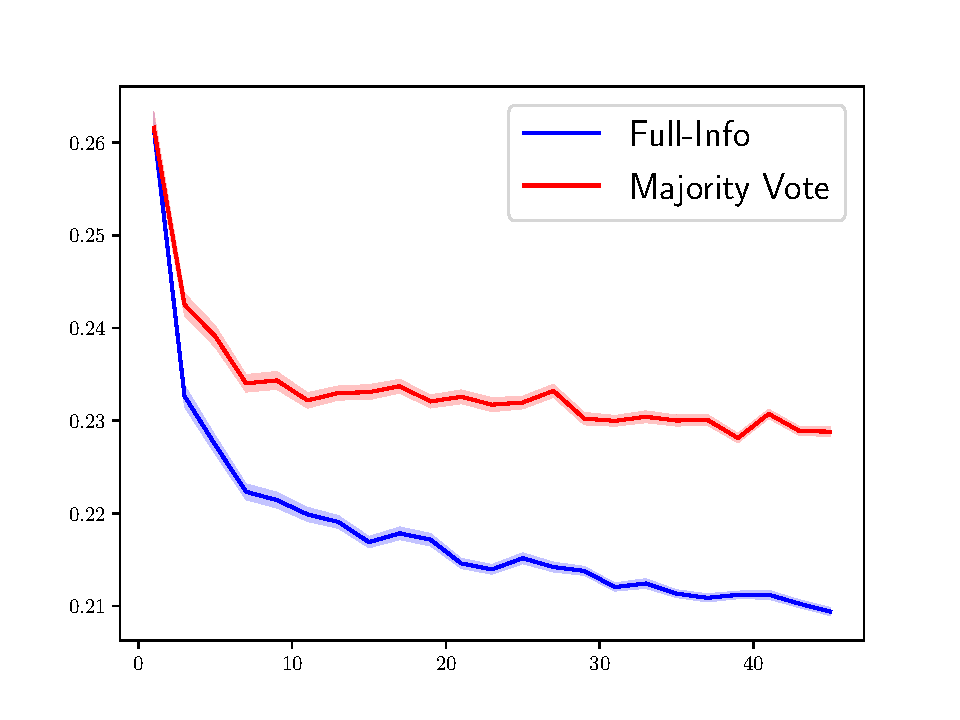
\includegraphics[width=0.45\textwidth]{figure/resnet-class-new.pdf}
			%		& 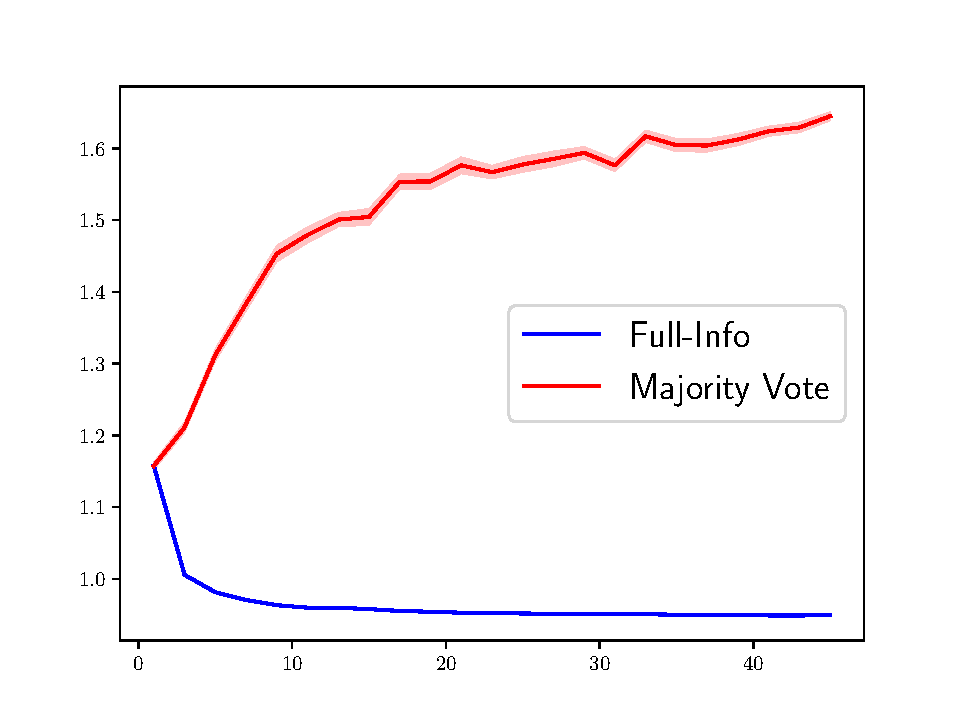
\includegraphics[width=0.45\textwidth]{figure/resnet-calib-new.pdf} \\
			%		(a) & (b) 
			%	\end{tabular}
		%	\caption{Experiments on CIFAR-10H dataset with (a) classification error and (b) calibration error with ResNet features when $d=40$. The classification error is the $0$-$1$ error compared to true labels. The calibration error is measured by $|\mathsf{logit}(\tilde{p}_i) - \mathsf{logit}(\hat{p}_i)|$ where $\tilde{p}_i$ is the predicted probability and $\hat{p}_i$ is the empirical probability. The errors are measured by ten-fold cross-validation. For each fixed $m$, we create $m$ labels for each image by subsampling and average over 100 trials. The error bars show 95\% confidence bands.} \label{fig:cifar}
		%\end{figure}
\input{lower-bound-supp.tex}
\section{Technical lemmas} \label{sec:technical}

We collect several technical lemmas and their proofs in this section, which
will be helpful in the main proofs. See
Appendices~\ref{proof:Sigma-inverse}, \ref{proof:t-Z-integral-noise},
\ref{proof:m-rho-integral-noise-general} and
\ref{proof:rademacher-symmetrization} for their proofs.

\begin{lemma} \label{lem:Sigma-inverse}
  Suppose $A, B \in \mathbb{R}^{d \times d}$ are symmetric, $AB = BA = 0$
  and the matrix $A+B$ is invertible. Then
  \begin{align*}
    \left(A +B\right)^{-1} = A^\dagger + B^\dagger.
  \end{align*}
\end{lemma}

The next two lemmas characterize asymptotic behaviors of expectations
involving a fixed function $f$ and some random variable $Z$ that satisfies
Assumption~\ref{assumption:z-density} for given $\beta>0$ and $c_Z <
\infty$. To facilitate stating the theorems, we recall
that such $Z$ are $(\beta,
c_Z)$-regular.
\begin{lemma} \label{lem:t-Z-integral-noise}
  Let $\beta > 0$ and $f$ be a function on $\R_+$ such that
  $z^{\beta-1}f(z)$ is integrable. If $Z$ is $(\beta,
  c_Z)$-regular (Assumption~\ref{assumption:z-density}), then
  \begin{align*}
    \lim_{t \to \infty} t^\beta \Ep [f(t|Z|)] =  c_Z \int_{0}^{\infty} z^{\beta - 1} f(z) dz.
  \end{align*}
\end{lemma}

\begin{lemma} \label{lem:m-rho-integral-noise-general}
  Let $\beta > 0$ and $c_Z < \infty$, and $Z$ be $(\beta, c_Z)$-regular, let
  $f : \R_+ \to \R$ satisfy $|f(z)| \leq a_0 + a_p z^p$ for some $a_0, a_p <
  \infty$ and all $z \in \R$, and assume $|Z|$ has finite $p$th
  moment. Additionally let $\rho_m(t)$ be the majority vote prediction
  function~\eqref{eq:link-function-m-majority-vote-general} and
  Assumption~\ref{assumption:condition-misspcfd-link-majority-vote} hold for
  each $\sigma_j\opt$ with limiting average derivative
  ${\wb{\sigma}\opt}'(0)$ at zero. Then for any $c > 0$
  \begin{align*}
    \lim_{m \to \infty} m^{\frac{\beta}{2}}\Ep \left[f(\sqrt{m}|Z|) (1 - \rho_m(cZ))\right] = c_Z \int_0^\infty z^{\beta - 1} f(z) \Phi \left(-2 {\wb{\sigma}\opt}'(0) cz\right) dz,
  \end{align*}
  where $\Phi(z) = \int_{-\infty}^z \frac{1}{\sqrt{2 \pi}}
  e^{-\frac{t^2}{2}}dt$ is the standard normal cumulative distribution function.
\end{lemma}

The fourth lemma is a uniform convergence result for the empirical risk in
the case that we have potentially distinct link functions
(cf.~Sec.~\ref{sec:master-results-sem}).
\begin{lemma}
  \label{lemma:rademacher-symmetrization}
  Assume $\E[\ltwo{X}^{\gamma}] \le M^\gamma$ for some $M \ge 1$ and $\gamma
  \ge 2$ and let the radius $1 \le r < \infty$. Let $\Flink \subset \{\sigma
  : \R \to [0, 1], \lipnorm{\sigma} \le \lipconst\}$.  Then for a constant
  $C \lesssim \sqrt{d \lipconst}$, we have
  \begin{equation*}
    \E\left[\sup_{\ltwo{\theta} \le r}
      \sup_{\vec{\sigma} \in \Flink^m} |P_n \loss_{\vec{\sigma},\theta} - L(\theta,
      \vec{\sigma})|\right]
    \le C \cdot
    (M r)^\frac{4\gamma}{3\gamma + 1} 
    \left(\frac{m}{n}\right)^\frac{\gamma}{3\gamma + 1}
    \sqrt{\log(rn)}.
  \end{equation*}
\end{lemma}


\subsection{Proof of Lemma~\ref{lem:Sigma-inverse}}
\label{proof:Sigma-inverse}

As $AB=BA=0$, the symmetric matrices $A$ and $B$ commute and so are
simultaneously orthogonally diagonalizable~\cite[Thm.~4.5.15]{HornJo85}. As
$AB=BA=0$, we can thus write
\begin{align*}
	A = U \begin{bmatrix} \Lambda_1 & 0 \\ 0 & 0 \end{bmatrix} U^\top  , \qquad B = U \begin{bmatrix} 0 & 0 \\ 0 & \Lambda_2 \end{bmatrix} U^\top  ,
\end{align*}
for some orthogonal $U \in \R^{d \times d}$, and as $A+B$ is invertible,  $\Lambda_1, \Lambda_2$ are invertible diagonal matrices. We conclude the proof by writing
\begin{align*}
	(A+ B)^{-1} = U \begin{bmatrix} \Lambda_1^{-1} & 0 \\ 0 & \Lambda_2^{-1} \end{bmatrix} U^\top = U \begin{bmatrix} \Lambda_1^{-1} & 0 \\ 0 & 0 \end{bmatrix} U^\top + U \begin{bmatrix} 0 & 0 \\ 0 & \Lambda_2^{-1} \end{bmatrix} U^\top = A^\dagger + B^\dagger .
\end{align*}

\subsection{Proof of Lemma~\ref{lem:t-Z-integral-noise}}  \label{proof:t-Z-integral-noise}
By the change of variables $w =t z$, we have
\begin{align*}
	t^\beta \Ep [f(t|Z|)] & = \int_{0}^{\infty} f(t z) \cdot t^{\beta - 1} p(z)  \cdot td z =  \int_{0}^{\infty} f(w) \cdot t^{\beta-1} p (w/t) d w \\
	& =  \int_{0}^{\infty} w^{\beta - 1} f(w) \cdot (w/t)^{1-\beta} p (w/t) d w.
\end{align*}
As $|  w^{\beta - 1} f(w) \cdot (w/t)^{1-\beta} p (w/t)| \leq \sup_{z \in (0, \infty)} z^{1-\beta} p(z) \cdot |w^{\beta - 1} f(w)|$, where $w^{\beta - 1} f(w)$ is integrable by assumption, we can invoke dominated convergence to see that
\begin{align*}
	\lim_{t \to \infty} t^\beta \Ep [f(t|Z|)] = \int_{0}^{\infty} w^{\beta - 1} f(w) \cdot \lim_{t \to \infty} (w/t)^{1-\beta} p (w/t) d w = c_Z \int_{0}^{\infty} w^{\beta - 1} f(w) dw.
\end{align*}

\subsection{Proof of Lemma~\ref{lem:m-rho-integral-noise-general}} \label{proof:m-rho-integral-noise-general}
By rescaling arguments, it suffices to prove the theorem for any function
$f$ satisfying
$|f(z)| \leq 1 + z^p$ on $\R_+$ for any $p \in \N$ such that $|Z|$
has finite $p$th moment.  For such $f$, we wish to
show
\begin{align*}
  \lim_{m \to \infty} m^{\frac{\beta}{2}} \Ep \left[f(\sqrt{m}|Z|) (1 - \rho_m(c Z))\right] = c_Z \int_0^\infty z^{\beta-1} f(z) \Phi \left(-2 {\wb{\sigma}\opt}'(0) c z\right) dz,
\end{align*}
where $\Phi$ is the standard normal cdf. The key insight is that we can
approximate $1 - \rho_m(t)$ by a suitable Gaussian cumulative distribution
function (recognizing that $\rho_m(t) > \half$ for $t \neq 0$ by
definition~\eqref{eq:link-function-m-majority-vote-general} as the
probability the majority vote is correct given margin
$\<\theta\opt, X\> = t$).

We first assume $Z \geq 0$ with probability $1$, as the general result
follows by writing $Z = (Z)_+ - (-Z)_+$.  We decompose into two
expectations, depending on $Z$ being large or small:
\begin{align}
  \lefteqn{m^{\frac{\beta}{2}} \Ep \left[f(\sqrt m |Z|) (1 - \rho_m(cZ)) \right]}
  \nonumber \\
  & = \underbrace{m^{\frac{\beta}{2}} \Ep \left[f(\sqrt m Z) (1 - \rho_m(cZ)) \ind\left\{0 \leq Z \leq \frac{M}{\sqrt m}\right\} \right]}_{\mathrm{(I)}} + \underbrace{m^{\frac{\beta}{2}} \Ep \left[f(\sqrt m Z) (1 - \rho_m(cZ)) \ind\left\{Z > \frac{M}{\sqrt m}\right\} \right]}_{\mathrm{(II)}}   .  \label{eq:normal-mid-main}
\end{align}
The proof consists of three main parts. 
\begin{enumerate}[leftmargin=2em,label=\arabic*.]
\item We approximate $1-\rho_m(t)$ by a Gaussian cdf.
\item We can approximate term (I) by replacing $1-\rho_m(t)$ with
  the Gaussian cdf, showing that
  \begin{align}
    \left|\lim_{m \to \infty} \mathrm{(I)} - c_Z \int_0^\infty z^{\beta - 1} f(z) \Phi \left( - 2{\wb{\sigma}\opt}'(0) cz \right) dz \right| = o_M(1)   . \label{eq:normal-mid-3}
  \end{align} 
\item For term (II), we show $1- \rho_m(cz)$ is small when $Z > M/\sqrt{m}$, which allows us to show that
  \begin{equation*}
    \limsup_{m \to \infty}
    \left|\mathrm{(II)} \right| = o_M(1).
  \end{equation*}
\end{enumerate} 
Thus by adding the two preceding displays and taking $M \to \infty$, we
obtain the lemma.

\newcommand{\linkstd}{\sigma_m^{\textup{std}}}

Before we dive into further details, we use the shorthand functions
\begin{equation}
  \linkstd(z)
  \defeq, \frac{\sum_{j=1}^m \prns{\sigma_j\opt(cz) - \half}}{\sqrt{\sum_{j=1}^m \sigma_j\opt(cz)\prns{1 - \sigma_j\opt(cz)}}},
  ~~~
  \Delta_m(z) \defeq 1 - \rho_m(cz) - \Phi(- \linkstd(z))
  \label{eqn:std-link},
\end{equation}
and we also write $p_\infty(\beta) := \sup_{z \in (0, \infty)} z^{1-\beta}
p(z) < \infty$.

\paragraph{Part 1. Normal approximation for $1- \rho_m(t)$ when $t = O(1/\sqrt{m})$.} Let $p_j = \sigma_j\opt(t)$ for shorthand and $Y_j \sim \mathrm{Bernoulli}(p_j)$ be independent random variables. For $t > 0$, then
\begin{align*}
  1 - \rho_m(t) & = \Prb \prn{Y_1 + \cdots + Y_m < \half} = \Prb
  \prn{\frac{\sum_{j=1}^m (Y_j - p_j)}{\sqrt{\sum_{j=1}^m p_j
        (1-p_j)}} < - \frac{\sum_{j=1}^m (p_j - \half)}{
      \sqrt{\sum_{j=1}^m p_j (1-p_j)}}} .
\end{align*}
Consider the centered and standardized random variables $\xi_j = (Y_j - p_j)/\sqrt{\sum_{j=1}^m p_j (1-p_j)} $ so that $\xi_1, \dots, \xi_m$ are zero mean, mutually independent, and satisfy
\begin{align*}
  \sum_{j=1}^m \var \prn{\xi_j} & = 1  , \\
  \sum_{j=1}^m \Ep \brk{\left|\xi_j\right|^3} & =
  \frac{\sum_{j=1}^m p_j (1-p_j)(p_j^2 + (1-p_j)^2)}{\prns{\sum_{j=1}^m p_j (1-p_j)}^{3/2}}
  \leq \frac{\max_{1 \leq j \leq m} (p_j^2 + (1-p_j)^2)}{\sqrt{\sum_{j=1}^m p_j(1-p_j)}}  .
\end{align*} 
By the Berry-Esseen theorem (cf.~\citet{ChenGoSh10, Shevtsova14}), for all
$t > 0$
\begin{align*}
	\left|1 - \rho_m(t) - \Phi \left(-\frac{ \sum_{j=1}^m \left( p_j - \half\right)}{\sqrt{\sum_{j=1}^m p_j (1-p_j)}}\right)\right| \leq \frac{3}{4} \cdot \frac{\max_{1 \leq j \leq m} (p_j^2 + (1-p_j)^2)}{\sqrt{\sum_{j=1}^m p_j (1-p_j)}}  .
\end{align*}
%
Fix any $M <\infty$. Then for $0 \leq t \leq cM /\sqrt m$ and large enough
$m$, the right hand side of the preceding display has the upper bound
$2/\sqrt{m}$, as in numerator we have $p_j^2 + (1-p_j)^2 \leq 1$, and in
denominator $\min_{1 \leq j \leq m}p_j(1-p_j) \to 1/4$ for all $j$ as $m \to
\infty$, which follows from
Assumption~\ref{assumption:condition-misspcfd-link-majority-vote}
that
\begin{equation*}
  \half \leq \limsup_{m \to \infty} \max_{1 \leq j \leq m} p_j \leq \limsup_{m \to \infty} \sup_{1 \leq j < \infty} {\sigma_j\opt} \prn{\frac{cM}{\sqrt m} } =
  \half.
\end{equation*}
By repeating the same argument for $-cM /\sqrt m \leq t < 0$, we obtain that for large $m$ and $|t| \leq cM / \sqrt m$,
\begin{align}
  \left|1 - \rho_m(t) - \Phi \left(-\left|\frac{ \sum_{j=1}^m \left( \sigma_j\opt(t) - \half\right)}{\sqrt{\sum_{j=1}^m \sigma_j\opt(t) \prn{1 - \sigma_j\opt(t)}}}\right|\right)\right| \leq \frac{2}{\sqrt m}   . \label{eq:BE-approximation}
\end{align}

\paragraph{Part 2. Approximating (I) by Gaussian cdf.}
For the first term (I) in~\eqref{eq:normal-mid-main}, we further decompose into a normal approximation term and an error term,
\begin{align*}
  \mathrm{(I)} = \underbrace{m^{\frac{\beta}{2}}
    \Ep \left[f(\sqrt m Z)\Phi(-\linkstd(z))
      \ind\left\{0 \leq Z \leq \frac{M}{\sqrt m}\right\} \right]}_{\mathrm{(III)}} + \underbrace{m^{\frac{\beta}{2}} \Ep \left[f(\sqrt m Z)\Delta_m(z) \ind\left\{0 \leq Z \leq \frac{M}{\sqrt m}\right\} \right]}_{\mathrm{(IV)}}, %\label{eq:normal-mid-0}
\end{align*}
where $\Delta_m(z) = 1 - \rho_m(cz) - \Phi(-\linkstd(z))$ as in
def.~\eqref{eqn:std-link}. We will show $\mathrm{(IV)} \to 0$ and so
$\mathrm{(III)}$ dominates. By the change of variables $w = \sqrt{m}z$, we can
further write (III) as
\begin{align*}
  \mathrm{(III)} 
  & = m^{\frac{\beta}{2}} \int_0^{\frac{M}{\sqrt m}} f(\sqrt m z) \Phi
  ( -\linkstd(z)) \cdot p(z) d z \nonumber \\
  & = \int_0^{M} w^{\beta - 1} f(w) \Phi  \left( - \linkstd\prn{\frac{w}{\sqrt m}}\right) \cdot  (w/\sqrt{m})^{1-\beta} p(w/\sqrt{m}) d w   .
\end{align*}
We want to take the limit $m \to \infty$ and apply dominated convergence
theorem. Because $(w/\sqrt{m})^{1-\beta} p(w/\sqrt{m}) \leq p_\infty(\beta)
< \infty$ and $\linkstd(w/\sqrt m) \geq 0$, we have
\begin{align*}
	&  w^{\beta - 1} f(w) \Phi  \left( - \linkstd\prn{\frac{w}{\sqrt m}}\right) \cdot  \left( - \linkstd\prn{\frac{w}{\sqrt m}}\right) \cdot  (w/\sqrt{m})^{1-\beta} p(w/\sqrt{m}) \leq w^{\beta - 1} f(w) \cdot \Phi(0) p_\infty(\beta)   .
\end{align*} 
As $\beta > 0$ and $|f(w)| \leq 1 + w^p$, $w^{\beta - 1} f(w)$ is integrable
on $[0, M]$, and by~\eqref{ass:misspcfd-link-1} and \eqref{ass:misspcfd-link-3}
  in Assumption~\ref{assumption:condition-misspcfd-link-majority-vote},
\begin{align*}
	\lim_{m \to \infty} \linkstd\prn{\frac{w}{\sqrt m}} & = \lim_{m \to \infty}\frac{\sqrt{m}\left(\wb{\sigma}_m\opt\prn{\frac{cw}{\sqrt m}}-\frac{1}{2}\right)}{\sqrt{ \frac{1}{m} \sum_{j=1}^m \sigma_j\opt\prn{\frac{cw}{\sqrt m}}\prn{1 - \sigma_j\opt\prn{\frac{cw}{\sqrt m}}}}} =  2 {\wb{\sigma}\opt}'(0) cw   .
\end{align*}
Using the above display and that $\lim_{m \to \infty} (w/\sqrt{m})^{1-\beta}
p(w/\sqrt{m}) = c_Z$, we can thus apply dominated convergence theorem
to conclude that
\begin{align*}
	\lim_{m \to \infty}\mathrm{(III)} 
%	&  = \int_0^{M} w^{\beta - 1} f(w) \cdot   \Phi  \left( -\lim_{m \to \infty} \linkstd(z)\right) \cdot \lim_{m \to \infty} w^{\beta - 1}m^{\frac{\beta - 1}{2}} p(wm^{-\frac{1}{2}}) d w \nonumber \\
	&  = c_Z \int_0^M w^{\beta - 1} f(w) \cdot  \Phi  \left( - 2 {\wb{\sigma}\opt}'(0) cw\right) dw = c_Z \int_0^\infty w^{\beta - 1} f(w) \Phi \left( - 2{\wb{\sigma}\opt}'(0) cw \right) dw + o_M(1). %\label{eq:normal-mid-1}
\end{align*} 

Next we turn to the error term (IV). By the
bound~\eqref{eq:BE-approximation}, $|\Delta_m(z)| \leq 2/\sqrt{m}$ when $|z|
\leq M/\sqrt{m}$ for large enough $m$, and substituting $w = \sqrt{m}z$,
\begin{align*}
	|\mathrm{(IV)}| & \leq m^{\frac{\beta}{2}} \Ep \left[|f(\sqrt m Z)| \cdot \frac{2}{\sqrt m} \cdot \ind\left\{0 \leq Z \leq \frac{M}{\sqrt m}\right\}   \right] \nonumber \\
	& = \frac{2}{\sqrt m} \int_0^{\frac{M}{\sqrt m}} \sqrt m \cdot |f(\sqrt m z)| \cdot m^{\frac{\beta-1}{2}} p(z) dz  = \frac{2}{\sqrt m} \int_0^M w^{\beta - 1}|f(w)| \cdot(w/\sqrt{m})^{1-\beta} p(w/\sqrt{m}) dw.
\end{align*}
By using Assumption~\ref{assumption:z-density} again that $(w/\sqrt{m})^{1-\beta} p(w/\sqrt{m}) \leq p_\infty(\beta) < \infty$, we further have
\begin{equation*}
  |\mathrm{(IV)}| 
  \leq \frac{2p_\infty(\beta) }{\sqrt m} \cdot \int_0^M w^{\beta - 1}|f(w)| dw
  \leq  \frac{2p_\infty(\beta) }{\sqrt m} \cdot
  \prn{\frac{M^\beta}{\beta} +\frac{M^{p+\beta}}{p+\beta}}
  \to 0,
\end{equation*}
where we use $|f(w)| \leq 1+w^p$. We have thus shown the
limit~\eqref{eq:normal-mid-3}.

%Substitute Eqs.~\eqref{eq:normal-mid-1} and \eqref{eq:normal-mid-2} into Eq.~\eqref{eq:normal-mid-0}, we obtain
%\begin{align*}
%	\left|\lim_{m \to \infty} \mathrm{(I)} - c_Z \int_0^\infty w^{\beta - 1} f(w) \Phi \left( - 2{\wb{\sigma}\opt}'(0) cw \right) dw \right| = o_M(1)   .
%\end{align*} 
\paragraph{Part 3. Upper bounding (II).}
In term~(II), when $Z$ is large, the key is that the quantity
$1-\rho_m(t)$ is
small when $|t| \geq cM /\sqrt{m}$: Hoeffding's
inequality implies the tail bound
\begin{align*}
  0 \leq 1 - \rho_m(t) \leq e^{-2 \left(\wb{\sigma}_m\opt(t) - \half\right)^2 m}  .
\end{align*}
Thus
\begin{align}
	|\mathrm{(II)}| &\leq  \int_{\frac{M}{\sqrt m}}^1 \sqrt m |f(\sqrt m z)|  e^{-2\left(\wb{\sigma}_m\opt(cz) - \half\right)^2m}\cdot  m^{\frac{\beta-1}{2}} p(z) dz + \int_{1}^\infty m^{\frac \beta 2} |f(\sqrt m z)|  e^{-2\left(\wb{\sigma}_m\opt(cz) - \half\right)^2m}\cdot  p(z) dz   . \nonumber  
\end{align}
Using the assumption that $\gamma \defeq\liminf_m \inf_{t \geq c}
\prn{\wb{\sigma}_m\opt(t) - \half} > 0$ from~\eqref{ass:misspcfd-link-2},
that $|f(z)| \leq 1 +z^p$ and $|Z|$ has finite $p$th moment, we observe
that
\begin{align*}
	\int_{1}^\infty m^{\frac \beta 2} |f(\sqrt m z)|  e^{-2\left(\wb{\sigma}_m\opt(cz) - \half\right)^2m}\cdot  p(z) dz\leq  m^{\frac{1}{2}(\beta + p)}  e^{-2\gamma^2m} \int_1^\infty (1 + z^p) p(z) dz \to 0  ,
\end{align*}
and consequently
\begin{align*} 
	\limsup_{m \to \infty} |\mathrm{(II)}|  & \leq  \limsup_{m \to \infty} \int_{\frac{M}{\sqrt m}}^1 \sqrt m |f(\sqrt m z)|  e^{-2\left(\wb{\sigma}_m\opt(cz) - \half\right)^2m}\cdot  m^{\frac{\beta-1}{2}} p(z) dz \nonumber \\
	& = \limsup_{m \to \infty}   \int_{M}^{\sqrt{m}}  w^{\beta - 1} |f(w)| e^{-2\left(\wb{\sigma}_m\opt\prn{\frac{cw}{\sqrt m}} - \half\right)^2m} \cdot (w/\sqrt{m})^{1-\beta} p(w/\sqrt{m}) d w   .
\end{align*}
For $w \in [M, \sqrt m]$, we have
\begin{align*}
	\left(\wb{\sigma}_m\opt\prn{\frac{cw}{\sqrt m}} - \half\right)^2m & = \left(\frac{\wb{\sigma}_m\opt\prn{\frac{cw}{\sqrt m}} - \half}{\frac{cw}{\sqrt m}}\right)^2 c^2 w^2 \geq \left(\inf_{0 < t \leq c} \frac{\wb{\sigma}_m\opt(t) - \half}{t}\right)^2 c^2 w^2   ,
\end{align*}
while Assumption~\eqref{ass:misspcfd-link-2} gives $\delta:=\inf_{0 < t \leq c} \frac{\wb{\sigma}_m\opt(t) - \half}{t} > 0$,  so
\begin{align*}
\limsup_{m \to \infty} |\mathrm{(II)}| & \leq \int_{M}^{\sqrt{m}}  w^{\beta - 1} |f(w)| e^{-\delta w^2} \cdot (w/\sqrt{m})^{1-\beta} p(w/\sqrt{m}) d w. %\label{eq:normal-mid-4}
\end{align*}
Using the inequality
$(w/\sqrt{m})^{1-\beta} p(w/\sqrt{m}) \leq p_\infty(\beta) < \infty$, we
apply dominated convergence:
\begin{align*}
  \lim_{m \to \infty} \int_{M}^{\sqrt{m}}  w^{\beta - 1} |f(w)| e^{-\delta w^2} \cdot (w/\sqrt{m})^{1-\beta} p(w/\sqrt{m}) d w  = c_Z \int_M^\infty  w^{\beta - 1}  |f(w)| e^{-\delta w^2} dw = o_M(1).
\end{align*}

\subsection{Proof of Lemma~\ref{lemma:rademacher-symmetrization}} \label{proof:rademacher-symmetrization}
We follow a typical symmetrization approach, then construct a covering
that we use to prove the lemma.
Let $P_n^0 = n^{-1} \sum_{i = 1}^n \varepsilon_i 1_{X_i, Y_i}$ be the
(random) symmetrized measure with point masses at $(X_i, Y_i)$ for
$Y_i = (Y_{i1}, \ldots, Y_{im})$. Then by a standard symmetrization
argument, we have
\begin{equation}
	\label{eqn:symmetrization-step}
	\E\left[\sup_{\ltwo{\theta} \le r}
	\sup_{\vec{\sigma} \in \Flink^m} |P_n \loss_{\vec{\sigma},\theta} - L(\theta,
	\vec{\sigma})|\right]
	\le 2 \E\left[\sup_{\ltwo{\theta} \le r}
	\sup_{\vec{\sigma} \in \Flink^m} \left|P_n^0 \loss_{\vec{\sigma}, \theta}
	\right|\right].
\end{equation}

We use a covering argument to bound the symmetrized
expectation~\eqref{eqn:symmetrization-step}.  Let $R < \infty$ to be
chosen, and for an (again, to be determined) $\epsilon > 0$ let $\mc{G}
\subset \Flink$
denote an $\epsilon$-cover of $\Flink$ in the supremum norm on $[-R, R]$,
that is, $\norm{g - \sigma} = \sup_{t \in [-R,R]} |g(t) - \sigma(t)|$, and
so for each $\sigma \in \Flink$ there exists $g \in \mc{G}$ such that
$\norm{g - \sigma} \le \epsilon$. Then~\cite[Ch.~2.7]{VanDerVaartWe96} we
have $\log \card(\mc{G}) \le O(1) \frac{R \lipconst}{\epsilon}$. Let
$\Theta_\epsilon$ be a minimal $\epsilon$-cover of $\{\theta \mid
\ltwo{\theta} \le r\}$ in $\ltwo{\cdot}$, so that $\log
\card(\Theta_\epsilon) \le d \log(1 + \frac{2r}{\epsilon})$
and $\max_{\theta \in \Theta_\epsilon} \ltwo{\theta} \le r$.
We claim that for each $\ltwo{\theta} \le r$ and $\sigma
\in \Flink$, there exists
$v \in \Theta_\epsilon$ and $g \in \mc{G}$ such that
\begin{equation}
	\left|\frac{1}{n} \sum_{i = 1}^n \varepsilon_i
	\left(\loss_{\sigma, \theta}(Y_{ij} \mid X_i)
	-
	\loss_{g, v}(Y_{ij} \mid X_i)\right)
	\right|
	\le \epsilon +
	\frac{1}{n}\sum_{i = 1}^n \ltwo{X_i} \epsilon
	+ \frac{1}{n} \sum_{i = 1}^n\indic{\ltwo{X_i} \ge R / r}.
	\label{eqn:covering-diff}
\end{equation}
Indeed, for any $g \in \Flink$ and $\theta, v \in \R^d$, we have
\begin{align*}
	\left|\loss_{\sigma, \theta}(y \mid x)
	- \loss_{g, v}(y \mid x)\right|
	& = \left|\int_0^{y \<x, \theta\>} \sigma(-t) dt
	- \int_0^{y \<x, v\>} g(-t) dt\right| \\
	& \le \sup_{|t| \le r \ltwo{x}} |\sigma(t) - g(t)|
	+ \left|\int_{y\<x, v\>}^{y\<x, \theta\>}
	|\sigma(-t) - g(-t)| dt \right| \\
	& \le \norm{\sigma - g} + \indic{\ltwo{x} \ge R/r}
	+ |\<x, \theta - v\>| \\
	& \le
	\norm{\sigma - g} + \ltwo{x} \ltwo{\theta - v}
	+ \indic{\ltwo{x} \ge R/r},
\end{align*}
where we have used that $\sigma, g \in [0, 1]$.
Taking the elements $g, v$ in the respective coverings to minimize
the above bound gives the guarantee~\eqref{eqn:covering-diff}.

We now leverage inequality~\eqref{eqn:covering-diff}
in the symmetrization step~\eqref{eqn:symmetrization-step}.
We have
\begin{align*}
	\lefteqn{\E\left[\sup_{\ltwo{\theta} \le r}
		\sup_{\vec{\sigma} \in \Flink^m} |P_n \loss_{\vec{\sigma},\theta} - L(\theta,
		\vec{\sigma})|\right]} \\
	& \lesssim
	\E\left[\max_{\theta \in \Theta_\epsilon}
	\max_{\vec{g} \in \mc{G}^m}
	\left|P_n^0 \loss_{\vec{g}, \theta}\right|
	\right]
	+ \epsilon + \E[\ltwo{X_1}] \epsilon
	+ \frac{1}{n} \sum_{i = 1}^n \P(\ltwo{X_i} \ge R / r) \\
	& \stackrel{(i)}{\lesssim}
	\sqrt{\frac{d m R \lipconst}{\epsilon}
		\log\left(1 + \frac{2r}{\epsilon}\right)}
	\E\left[\frac{r^2}{n}\sum_{i = 1}^n \ltwo{X_i}^2\right]^{1/2}
	+ \epsilon + \E[\ltwo{X_1}] \epsilon
	+ \frac{\E[\ltwo{X_i}^{\gamma}]}{(R/r)^{\gamma}} \\
	& \le
	M r \sqrt{\frac{dm R \lipconst}{n \epsilon}
		\log \left(1 + \frac{2r}{\epsilon}\right)}
	+ (M + 1) \epsilon
	+ \frac{M^{\gamma}}{(R/r)^{\gamma}},
\end{align*}
where inequality $(i)$ uses that if $Z_i$ are $\tau^2$-sub-Gaussian, then
$\E[\max_{i \le N} |Z_i|] \le \sqrt{2 \tau^2 \log N}$, and that
conditional on $\{X_i, Y_i\}_{i = 1}^n$, the symmetrized sum $\sum_{i =
	1}^n \varepsilon_i \frac{1}{m} \sum_{j = 1}^m \loss_{g_j, \theta}(Y_{ij}
\mid X_i)$ is $r^2 \sum_{i = 1}^n \ltwo{X_i}^2$-sub-Gaussian, as
$|\loss_{g_j, \theta}(Y_{ij} \mid X_i)| \le |\<X_i, \theta\>| \le r
\ltwo{X_i}$.  We optimize this bound to get the final guarantee of the
lemma: set $\epsilon = (Rm / n)^{1/3}$ (and note that we will
choose $R \ge 1$) to obtain
\begin{equation*}
	\E\left[\sup_{\ltwo{\theta} \le r}
	\sup_{\vec{\sigma} \in \Flink^m} |P_n \loss_{\vec{\sigma},\theta} - L(\theta,
	\vec{\sigma})|\right]
	\lesssim \sqrt{d \lipconst \log(rn)}
	M r \left(\frac{R m}{n}\right)^{1/3}
	+ \frac{(Mr)^\gamma}{R^\gamma}.
\end{equation*}
Choose $R
= ((Mr)^{3(\gamma - 1)} n / m)^\frac{1}{3\gamma + 1}$.

%\subsection{Proof of Lemma~\ref{lemma:glivenko-cantelli}} \label{proof:glivenko-cantelli}
%We use a more or less standard Rademacher complexity and
%symmetrization argument. Let
%$\Prb_{n}'$ denote an independent copy of $\Prb_{n}$, that is, we draw
%independent copies $X_i'$ and, draw $Y_{ij}'$
%independently conditional on $X_i'$ according to the same distribution from which $Y_{ij} \mid X_i$ are drawn. Let $\varepsilon_i \in \{\pm 1\}$ be
%i.i.d.\ uniform signs. Then for any $1 \le k < \infty$,
%\begin{align*}
%	\Ep\left[\sup_{\ltwo{\theta} \le r, \eta \in \mathcal{E}} \left|\Prb_n\loss_{\theta, \eta} -
%	\Prb \loss_{\theta, \eta} \right|^k\right]
%	& \le \Ep\left[\sup_{\ltwo{\theta} \le r, \eta \in \mathcal{E}}
%	\left|(\Prb_{n} - \Prb_{n}') \loss_{\theta, \eta} \right|^k\right] \\
%	& \le 2^k \Ep\left[\sup_{\ltwo{\theta} \le r, \eta \in \mathcal{E}}
%	\left|\frac{1}{n} \sum_{i = 1}^n \varepsilon_i
%	\left(\frac{1}{m} \sum_{j = 1}^m \prn{h_{\eta, j}(Y_{ij} \<\theta, X_i\>)
%		- h_{\eta, j}(0) }\right)\right|^k\right],
%\end{align*}
%where the first inequality is Jensen's and the second adds and subtracts
%$\frac{1}{m} \sum_{j=1}^m h_{\eta, j}(0) = \loss_{0,\eta}$, then uses that $\frac{1}{m} \sum_{j = 1}^m h_{\eta, j}(Y_{ij} \<\theta, X_i\>) - \frac{1}{m} \sum_{j = 1}^m h_{\eta, j}(Y_{ij}' \<\theta, X_i'\>)$ is
%symmetric. Next apply Jensen's inequality once again for $|x|^k$ we have
%\begin{align*}
%	\Ep\left[\sup_{\ltwo{\theta} \le r, \eta \in \mathcal{E}} \left|\Prb_n\loss_{\theta, \eta} -
%	\Prb \loss_{\theta, \eta} \right|^k\right] \leq \frac{2^k}{m} \sum_{j=1}^m \Ep\left[\sup_{\ltwo{\theta} \le r, \eta \in \mathcal{E}}
%	\left|\frac{1}{n} \sum_{i = 1}^n \varepsilon_i
%	\left(\prn{h_{\eta, j}(Y_{ij} \<\theta, X_i\>)
%		- h_{\eta, j}(0) }\right)\right|^k\right]
%\end{align*}
%Applying the Rademacher contraction
%inequality~\cite[Thm.~4.12]{LedouxTa91},
%we thus obtain
%\begin{align*}
%	\Ep\left[\sup_{\ltwo{\theta} \le r, \eta \in \mathcal{E}} \left|\Prb_n\loss_{\theta, \eta} -
%	\Prb \loss_{\theta, \eta} \right|^k\right]
%	& \le \frac{4^k}{m} \sum_{j=1}^m \Ep\left[\sup_{\ltwo{\theta} \le r}
%	\left|\frac{1}{n} \sum_{i = 1}^n \varepsilon_i
%	\cdot \mathsf{L} Y_{ij} \<\theta, X_i\>\right|^k\right] \\
%	& = \frac{\prn{4\mathsf{L}r}^k}{m} \sum_{j=1}^m \Ep\left[
%	\ltwo{\frac 1 n\sum_{i = 1}^n \varepsilon_i X_i  Y_{ij}}^k
%	\right] \\
%	& \le \left(\frac{4 \mathsf{L}r \sqrt{k}}{n}\right)^k
%	\Ep\left[\left(\sum_{i = 1}^n \ltwo{X_i}^2\right)^{k/2}
%	\right],
%\end{align*}
%where the final inequality uses that $Y_{ij} \in \{\pm 1\}$ and standard
%Khintchine-type bounds in Hilbert spaces~\cite[Sec.~1.4]{delaPenaGi99}.
%Finally, we note that $\Ep[(\sum_{i = 1}^n \ltwo{X_i}^2)^{k/2}] \le n^{k/2}
%\frac{1}{n} \sum_{i = 1}^n \Ep[\ltwo{X_i}^{k}]$ for all $k \ge 2$ by
%Jensen's inequality. Applying
%Markov's inequality, for any $t \ge 0$ and $k \ge 1$,
%\begin{align*}
%	\Prb\left(\sup_{\ltwo{\theta} \le r}
%	\left|\Prb_{n,m}\loss_\theta - \poploss(\theta) \right| \ge t \right)
%	& \le \left(\frac{4 \mathsf{L} r \sqrt{k}}{t \sqrt{n}}\right)^k
%	\Ep[\ltwo{X_1}^k].
%\end{align*}
%For $k > 2$, this is summable, so that the Borel-Cantelli theorem gives
%a.s.\ convergence. Take $n \to \infty$ to get the result.


\section{Proof of Theorem~\ref{theorem:multilabel-asymptotics}}
\label{sec:proof-multilabel-asymptotics}

Let $t_m$ be the solution to $h_{t\opt,m}(t) = 0$ as in
Lemma~\ref{lemma:generic-solutions}. The consistency argument is
immediate: the losses $\loss$ are convex, continuous, and locally Lipschitz,
so~\citet[Thm.~5.4]{ShapiroDeRu09} gives $\what{\theta}_n
\cas \theta\opt_L$. By an appeal to standard
M-estimator theory~\cite[e.g.][Thm.~5.23]{VanDerVaart98},
we thus obtain
\begin{equation}
	\label{eqn:multilabel-basic-asymptote}
	\sqrt{n} \big(\what{\theta}_n - \theta\opt_L\big)
	\cd \normal\left(0, \nabla^2 L(\theta\opt_L, \sigma)^{-1}
	\cov\bigg(\frac{1}{m} \sum_{j = 1}^m
	\nabla \loss_{\sigma,\theta\opt_L}(Y_j \mid X)\bigg)
	\nabla^2 L(\theta\opt_L, \sigma)^{-1} \right).
\end{equation}
We expand the covariance term to obtain the first main result of the
theorem. For shorthand, let $G_j = \nabla \loss_{\sigma,\theta\opt_L}(Y_j
\mid X)$, so that $\sum_{j = 1}^m \E[G_j] = 0$ and the $G_j$ are
conditionally independent given $X$. Applying the law of total covariance,
we have
\begin{align*}
	\cov\bigg(\frac{1}{m} \sum_{j = 1}^m G_j\bigg)
	& = \cov\bigg(\frac{1}{m} \sum_{j = 1}^m
	\E[G_j \mid X]\bigg)
	+ \E\left[\cov\bigg(
	\frac{1}{m} \sum_{j = 1}^m G_j \mid X\bigg)\right] \\
	& =
	\underbrace{\cov\bigg(\frac{1}{m} \sum_{j = 1}^m \E[G_j \mid X] \bigg)}_{
		\mathrm{(I)}}
	+ \frac{1}{m^2} \sum_{j = 1}^m
	\underbrace{\E\left[\cov(G_j \mid X)\right]}_{\mathrm{(II)}},
\end{align*}
where we have used the conditional independence of the $Y_j$ conditional on
$X$.  We control each of terms (I) and (II) in turn.

For the first, we have by the independent decomposition
$X = Z u\opt + \projperp W$ that
\begin{equation*}
	\E[G_j \mid X]
	= 
	\left(\sigma(t_m Z)
	(1 - \sigma_j\opt(t\opt Z))
	- \sigma(- t_m Z) \sigma_j\opt(t\opt Z)\right)
	X,
\end{equation*}
and so
\begin{align*}
	\mathrm{(I)} & =
	\E\left[\left(\sigma(t_m Z) (1 - \wb{\sigma}\opt(t\opt Z))
	- \sigma(-t_m Z) \wb{\sigma}\opt(t\opt Z)\right)^2 XX^\top \right] \\
	& =
	\E\left[\left(\sigma(t_m Z) (1 - \wb{\sigma}\opt(t\opt Z))
	- \sigma(-t_m Z) \wb{\sigma}\opt(t\opt Z)\right)^2 Z^2 \right]
	u\opt {u\opt}^\top
	\\ & \qquad ~ + 
	\E\left[\left(\sigma(t_m Z) (1 - \wb{\sigma}\opt(t\opt Z))
	- \sigma(-t_m Z) \wb{\sigma}\opt(t\opt Z)\right)^2\right]
	\projperp \Sigma \projperp \\
	& = \E[\linkerr(Z)^2 Z^2] u\opt {u\opt}^\top
	+ \E[\linkerr(Z)^2]   \projperp \Sigma \projperp,
\end{align*}
where we used the independence of $W$ and $Z$.
For term (II) above, we see that conditional on $X$,
$\nabla \loss_{\sigma,\theta}(Y_j \mid X)$ is a binary
random variable taking values in
$\{-\sigma(-t_m Z) X, \sigma(t_m Z) X\}$ with probabilities
$\sigma_j\opt(t\opt Z)$ and
$1 - \sigma_j\opt(t\opt Z)$, respectively, so that
a calculation leveraging the variance of Bernoulli random variables
yields
\begin{align*}
	\cov(G_j \mid X)
	& = \sigma_j\opt(t\opt Z) (1 - \sigma_j\opt(t\opt Z))
	\left(\sigma(t_m Z) + \sigma(-t_m Z)\right)^2 XX^\top
	= v_j(Z) XX^\top,
\end{align*}
where we used the definition~\eqref{eqn:error-functions} of the
variance terms.
A similar calculation to that we used for term (I) then gives that
\begin{align*}
	\mathrm{(II)} & = \frac{1}{m^2}
	\sum_{j = 1}^m \E[v_j(Z) Z^2] u\opt {u\opt}^\top
	+ \frac{1}{m^2}
	\sum_{j = 1}^m \E[v_j(Z)] \projperp \Sigma \projperp.
	%% \mathrm{(II)} & =
	%% \frac{1}{m^2} \sum_{j = 1}^m
	%% \E\left[\sigma_j\opt(t\opt Z) (1 - \sigma_j\opt(t\opt Z))
	%%   \left(\sigma(t_m Z) + \sigma(-t_m Z)\right)^2 Z^2 \right] u\opt {u\opt}^\top
	%% \\ & \qquad ~
	%% + \frac{1}{m^2} \sum_{j = 1}^m \E\left[
	%%   \sigma_j\opt(t\opt Z) (1 - \sigma_j\opt(t\opt Z))
	%%   \left(\sigma(t_m Z) + \sigma(-t_m Z)\right)^2\right]
	%% \projperp \Sigma \projperp.
\end{align*}
Applying Lemma~\ref{lem:Sigma-inverse} then allows us to decompose the the
covariance in expression~\eqref{eqn:multilabel-basic-asymptote} into
terms in the span of $u\opt {u\opt}^\top$ and those perpendicular to
it, so that the asymptotic covariance is
\begin{align*}
	\frac{\E[\linkerr(Z)^2 Z^2] + \frac{1}{m^2}
		\sum_{j = 1}^m \E[v_j(Z) Z^2]}{
		\E[\hessfunc(Z) Z^2]^2} u\opt {u\opt}^\top
	+ \frac{\E[\linkerr(Z)^2] + \frac{1}{m^2}
		\sum_{j = 1}^m \E[v_j(Z)]}{\E[\hessfunc(Z)]^2}
	\prn{\projperp \Sigma \projperp}^\dagger,
\end{align*}
by applying Lemma~\ref{lemma:generic-solutions} for the form of the Hessian
$\nabla^2 L(\theta_L\opt, \sigma)$ and Lemma~\ref{lem:Sigma-inverse} for the
inverse, giving the first result of the theorem.

To obtain the second result, we apply the delta method with
the mapping $\phi(x) = x / \ltwo{x}$, which satisfies
$\nabla \phi(x) = (I - \phi(x) \phi(x)^\top) / \ltwo{x}$,
so that for $\what{u}_n = \what{\theta}_n / \ltwos{\what{\theta}_n}$ we have
\begin{align*}
  \sqrt{n}(\what{u}_n - u\opt)
  & \cd
  \normal\left(0, \frac{1}{t_m^2}
  \frac{\E[\linkerr(Z)^2] + \frac{1}{m^2}
    \sum_{j = 1}^m \E[v_j(Z)]}{\E[\hessfunc(Z)]^2}
  \prn{\projperp \Sigma \projperp}^\dagger
  \right)
\end{align*}
as desired.

\subsection{Proof of Lemma~\ref{lemma:generic-solutions}}
\label{sec:proof-generic-solutions}

Recall that $h = h_{t\opt, m}$ is the calibration
gap function~\eqref{eqn:h-m-func}.
We see that because $\E[Z] = 0$, we have
$h(0) = -2 \E[Z \varphi_m(t\opt Z)] < 0$,
while using Assumption~\ref{assumption:model-link} and that
$\E[|Z|] < \infty$, we apply dominated convergence and that
$\lim_{t \to \infty} (\sigma(t Z) - \half) Z = c|Z|$ with probability 1
to obtain
\begin{align*}
	\lim_{t \to \infty} h(t) = \E[c|Z| (1 - \varphi_m(t\opt Z))]
	+ \E[c |Z| \varphi_m(t\opt Z)] = c \E[|Z|] > 0.
\end{align*}
Because $h'(t) = \E[\sigma'(tZ) Z^2 (1 - \varphi_m(t\opt Z))]
+ \E[\sigma'(-tZ) Z^2 \varphi_m(t\opt Z)] > 0$, we see that there
is a unique $t_m$ solving $h(t_m) = 0$, and evidently
$\theta\opt_L = t_m u\opt$ is a minimizer of $L$.

We compute the Hessian of $L$. For this,
we again let $\theta = t u\opt$ to write
\begin{align*}
	\nabla^2 L(\theta, \sigma) & = \E[\sigma'(-\<\theta, X\>) XX^\top \varphi_m(\<X, \theta\opt\>)]
	+ \E[\sigma'(\<\theta, X\>) XX^\top (1 - \varphi_m(\<X, \theta\opt\>))] \\
	& = \E\left[\sigma'(-t Z) \varphi_m(t\opt Z)
	\left(Z^2 u\opt {u\opt}^\top + WW^\top\right)\right]
	+ \E\left[\sigma'(t Z) (1 - \varphi_m(t\opt Z))
	\left(Z^2 u\opt {u\opt}^\top + WW^\top \right)\right] \\
	& = \E\left[\left(\sigma'(-tZ) \varphi_m(t\opt Z)
	+ \sigma'(tZ) (1 - \varphi_m(t\opt Z)) \right) Z^2\right]
	u\opt {u\opt}^\top \\
	& \quad + \E\left[\sigma'(-tZ) \varphi_m(t\opt Z)
	+ \sigma'(tZ) (1 - \varphi_m(t\opt Z))\right] \E[WW^\top],
\end{align*}
which gives $\nabla^2 L(\theta, \sigma) \succ 0$ and so $\theta\opt_L$ is
unique.  Finally, the desired form of the Hessian follows as $\E[WW^\top] =
\projperp \Sigma \projperp$.

\section{Proof of Theorem~\ref{theorem:majority-vote-asymptotics}}
\label{sec:proof-majority-vote-asymptotics}

As in the proof of Theorem~\ref{theorem:multilabel-asymptotics}, we begin
with a consistency result. Let $t_m$ be the solution to $h_{t\opt, m}(t) =
0$ as in Lemma~\ref{lemma:generic-solutions}.
The once again, \citet[Thm.~5.4]{ShapiroDeRu09}
shows that $\what{\theta}_n \cas \theta\opt_L$.
As previously, appealing to standard
M-estimator theory~\cite[e.g.][Thm.~5.23]{VanDerVaart98},
we obtain
\begin{equation}
	\label{eqn:vote-basic-asymptote}
	\sqrt{n} \big(\what{\theta}_n - \theta\opt_L\big)
	\cd \normal\left(0, \nabla^2 L(\theta\opt_L, \sigma)^{-1}
	\cov \left(\nabla \loss_{\sigma,\theta\opt_L}(\majY \mid X)\right)
	\nabla^2 L(\theta\opt_L, \sigma)^{-1} \right),
\end{equation}
the difference from the asymptotic~\eqref{eqn:multilabel-basic-asymptote}
appearing in the covariance term.
Here, we recognize that conditional on $X = Z u\opt + W$, the vector
$\nabla \loss_{\sigma,\theta\opt_L}(\majY \mid X)$
takes on the values
$\{-\sigma(-t_m Z) X, \sigma(t_m Z) X\}$ each with probabilities
$\varphi_m(t\opt Z)$ and $1 - \varphi_m(t\opt Z)$, respectively,
while $\nabla \loss_{\sigma,\theta\opt_L}(\majY \mid X)$ is (unconditionally)
mean zero.
Thus
we have
\begin{align*}
	\cov \left(\nabla \loss_{\sigma,\theta\opt_L}(\majY \mid X)\right)
	& = \E\left[\sigma(-t_m Z)^2 \varphi_m(t\opt Z) XX^\top
	+ \sigma(t_m Z)^2 (1 - \varphi_m(t\opt Z)) XX^\top\right] \\
	& = \E\left[\left(\sigma(- t_m Z)^2 \varphi_m(t\opt Z)
	+ \sigma(t_m Z)^2 (1 - \varphi_m(t\opt Z))\right) Z^2\right]
	u\opt{u\opt}^\top \\
	& \qquad ~ +
	\E\left[\sigma(- t_m Z)^2 \varphi_m(t\opt Z)
	+ \sigma(t_m Z)^2 (1 - \varphi_m(t\opt Z))\right]
	\projperp \Sigma \projperp.
\end{align*}

Applying Lemma~\ref{lem:Sigma-inverse}
as in the proof of Theorem~\ref{theorem:multilabel-asymptotics}
to  decompose the covariance
terms in the asymptotic~\eqref{eqn:vote-basic-asymptote}, and substituting in $\rho_m(t) = \sigma(t) \ind \{t \geq 0\} + (1- \sigma(t)) \ind \{t < 0\}$,
the limiting covariance in expression~\eqref{eqn:vote-basic-asymptote}
becomes
\begin{align*}
  & \frac{\E[(\sigma(-t_m |Z|)^2 \rho_m(t\opt Z) + \sigma(t_m |Z|)^2
      (1 - \rho_m(t\opt Z))) Z^2]}{
    \E[\hessfunc(Z) Z^2]^2}
  u\opt {u\opt}^\top \\
  & \qquad ~ + 
  \frac{\E[\sigma(-t_m |Z|)^2 \rho_m(t\opt Z) + \sigma(t_m |Z|)^2
      (1 - \rho_m(t\opt Z))]}{
    \E[\hessfunc(Z)]^2}
  \prn{\projperp \Sigma \projperp}^\dagger.
\end{align*}
Lastly, we apply the delta method to $\phi(x) = x / \ltwo{x}$,
exactly as in the proof of Theorem~\ref{theorem:multilabel-asymptotics},
which gives the theorem.

% -*- mode: latex -*- %
%\setcounter{theorem}{6}
%\setcounter{equation}{9}

\section{Proofs of asymptotic normality}

In this appendix, we include proofs of the convergence results in
Propositions~\ref{prop:lowd-maximum-likelihood},
\ref{prop:lowd-majority-vote-m-noise}, and
\ref{prop:lowd-misspcfd-majority-vote-m}. In each, we divide the proof into
three steps: we characterize the loss minimizer, apply one of the master
Theorems~\ref{theorem:multilabel-asymptotics}
or~\ref{theorem:majority-vote-asymptotics} to obtain asymptotic normality,
and then characterize the behavior of the asymptotic covariance as $m \to
\infty$.

\subsection{Proof of Proposition~\ref{prop:lowd-maximum-likelihood}}
\label{proof:lowd-maximum-likelihood}

\paragraph{Asymptotic normality of the MLE.}
The asymptotic
normality result is an
immediate consequence of the classical asymptotics for maximum likelihood
estimators~\cite[Thm.~5.29]{VanDerVaart98}.


\paragraph{Normalized estimator.}
For the normalized estimator, we appeal to the master results developed in Section~\ref{sec:master-results}.
%
In particular, since we are in the well-specified logistic model, we can invoke Corollary~\ref{cor:well-specified-normalized-cov} and write directly that
\begin{equation*}
	\sqrt{n}(\what{u}_{n,m}\lr- u\opt)
	\cd \normal\left(0, \frac{1}{m} \cdot
	\frac{1}{{t\opt}^2}
	\frac{\E[\sigma\lr(t\opt Z) (1 - \sigma\lr(t\opt Z))]}{\E[{\sigma\lr}'(t\opt Z)]^2}
	\projperp \Sigma \projperp \right),
\end{equation*}
which immediately implies
\begin{align*}
	C(t) & = \frac{1}{t^2}
	\frac{\E[\sigma\lr(t Z) (1 - \sigma\lr(t Z))]}{\E[{\sigma\lr}'(t Z)]^2} = \frac{1}{t^2\Ep\left[\frac{e^{t Z} }{(1 + e^{t Z})^2}\right]},
\end{align*}
and that further $ C(t) {t}^{2 - \beta} = {t}^{-\beta} \Ep[\frac{e^{t|Z|}
  }{(1 + e^{t |Z|})^2}]^{-1}$. To compute the limit when $t \to
\infty$, we invoke Lemma~\ref{lem:t-Z-integral-noise} and
we conclude that
\begin{align*}
  \lim_{t \to \infty} C(t) t^{2 - \beta} = \lim_{t\to \infty}
  \frac{1}{t^\beta \Ep[\frac{e^{t |Z|} }{(1 + e^{t |Z|})^2}]}
  = \frac{1}{ c_Z \int_{0}^{\infty} \frac{z^{\beta - 1} e^{z} }{(1 + e^{z})^2}
    dz}.
\end{align*}

\subsection{Proof of Proposition~\ref{prop:lowd-majority-vote-m-noise}}
\label{proof:lowd-majority-vote-m-noise}

\paragraph{Minimizer of the population loss.}
We can see identity~\eqref{eq:majority-vote-root} still holds with the
calibration gap $h(t) = h_m(t) = \E[|Z|(1 - \rho_m(t\opt |Z|))] -
\E[\frac{|Z|}{1 + e^{t|Z|}}]$ in Eq.~\eqref{eqn:h-centering} as $X-u\opt Z$
and $u\opt Z$ are independent. The function $h(t)$ is monotonically
increasing in $t$ with $h(\infty) =\Ep \brk{|Z|(1-\rho_m(t^\star |Z|))} >
0$, while $1 - \rho_m(t|Z|) \leq 1 - \rho_1(t|Z|) = \frac{1}{1 + e^{t|Z|}}$,
we must have $h(t^\star) \leq 0$. Therefore there must be a unique zero
point $t_m \ge t\opt$ of $h(t)$, and so $t_m u\opt$ is the unique minimizer
of the population loss $\poploss\mv_m(\theta)$.

\paragraph{Asymptotic variance.}
As $t_m$ solves $h_m(t_m) = 0$, 
Eq.~\eqref{eq:majority-vote-root} guarantees that $t_m u\opt$ is the global
minimizer of the population loss $\poploss\mv_m$. Appealing to
Theorem~\ref{theorem:majority-vote-asymptotics}, it follows that
$\what{\theta}\mv_{n,m} \cp t_m u\opt$, and
\begin{align*}
  \sqrt{n} (\what{u}\mv_{n,m} -  u^\star)&\cd \normal\left(0, \varfunc(t\opt)
  \prn{\proj_{u\opt} \Sigma \proj_{u\opt}}^\dagger\right)
\end{align*}
for the variance function~\eqref{eqn:generic-majority-covariance},
which in this case simplifies to
\begin{align*}
  \varfunc(t\opt)
  %% & = \frac{1}{t_m^2} \frac{\E[\sigma\lr(-t_m |Z|)^2
  %%     \rho_m(t Z) + \sigma\lr(t_m |Z|)^2 (1 - \rho_m(t Z))]}{
  %%   \E[{\sigma\lr}'(t_m Z)]^2} \nonumber \\
  & = \frac{\Ep[\frac{1}{(1 + e^{t_m|Z|})^2} \rho_m(t\opt |Z|)
      + \frac{1}{(1 + e^{-t_m|Z|})^2} (1-\rho_m(t\opt |Z|)) ]}{
    t_m^2 \Ep[\frac{e^{t_m Z} }{ (1 + e^{t_m Z})^2}]^2}
\end{align*}
via the symmetry $\rho_m(t) = \rho_m(-t)$.

\paragraph{Large $m$ behavior.} The remainder of the
proof is to characterize the behavior of $\varfunc(t\opt)$ as $m\to\infty$.
We first derive asymptotics for $t_m$. To simplify notation, we let
$\ltwo{\theta} = t = t\opt$. Because $t_m$ solves $h_m(t_m) = 0$ we have
\begin{align}
  \Ep \brk{\frac{|Z|}{1 + e^{t_m|Z|}}} = \Ep \brk{|Z|(1-\rho_m(t |Z|))},
  \label{eqn:solving-for-t-m}
\end{align}
we must have $t_m \to \infty$ as $m \to \infty$ because $\rho_m(t) \to 1$
for any $t > 0$ as $m \to \infty$, so the right side of
equality~\eqref{eqn:solving-for-t-m} converges to 0 by the dominated
convergence theorem, and hence so must the left hand side.  Invoking
Lemma~\ref{lem:t-Z-integral-noise} for the left hand side, it follows that
\begin{align*}
  \lim_{m \to \infty} t_m^{\beta + 1} \Ep \brk{\frac{|Z|}{1 + e^{t_m|Z|}}} & = \lim_{m \to \infty} t_m^{\beta} \Ep \brk{\frac{t_m|Z|}{1 + e^{t_m|Z|}}}  =  c_Z \int_{0}^{\infty} \frac{z^\beta}{1 + e^{z}} dz, %\label{eq:large-m-general-mid-1}
\end{align*}
while invoking Lemma~\ref{lem:m-rho-integral-noise-general} for the right
hand side of~\eqref{eqn:solving-for-t-m}, it follows that
\begin{align*}
  \lim_{m \to \infty} m^{\frac{\beta+1}{2}}\Ep \brk{|Z|(1-\rho_m(t  |Z|))} & = \lim_{m \to \infty} m^{\frac{\beta}{2}} \Ep \brk{\sqrt m|Z|(1-\rho_m(t  |Z|))} \nonumber \\
  &  = c_Z \int_0^\infty z^\beta \Phi \left(-\frac{tz}{2}\right) dz = c_Z {t}^{-\beta-1}\int_0^\infty z^\beta \Phi \left(-\frac{z}{2}\right) dz, %\label{eq:large-m-general-mid-2}
\end{align*}
where the last line follows from change of variables $tz \mapsto z$. The
identity~\eqref{eqn:solving-for-t-m}
implies that the ratio $\Ep [|Z|/(1 + e^{t_m|Z|})] / \Ep [|Z|(1-\rho_m(t
  |Z|))] = 1$ and so we have that as $m \to \infty$,
\begin{align*}
		\frac{t_m}{\sqrt{m}} & = \left(\frac{	t_m^{\beta + 1}}{ m^{\frac{\beta+1}{2}}}\right)^{\frac{1}{\beta +1}} =  \left(\frac{	t_m^{\beta + 1}\Ep \brk{\frac{|Z|}{1 + e^{t_m|Z|}}}}{ m^{\frac{\beta+1}{2}} \Ep \brk{|Z|(1-\rho_m(t |Z|))} }\right)^{\frac{1}{\beta +1}}  \to  \left(\frac{\int_{0}^{\infty} \frac{z^\beta}{1 + e^{z}} dz}{\int_0^\infty z^\beta \Phi \left(-\frac{z}{2}\right) dz}\right)^{\frac{1}{\beta +1}} \cdot t= : a t .  \label{eq:Cm-asymp-noise-tm}
\end{align*}
In particular, $t_m / t\opt \sqrt{m} = a(1 + o_m(1))$.

We finally proceed to compute asymptotic behavior of $\varfunc(t\opt)$, the
variance~\eqref{eqn:generic-majority-covariance}. By
Lemma~\ref{lem:t-Z-integral-noise} the limit of its denominator as $t_m \to
\infty$ satisfies
\begin{align*}
  \lim_{m \to \infty}
  \underbrace{t_m^{2 \beta}
    \Ep\left[\frac{e^{t_m Z} }{ (1 + e^{t_m Z})^2}\right]^2}_{
    :=\mathsf{den}(C_m(t))}
  & = \lim_{t \to \infty} \left( t^\beta \Ep\left[\frac{e^{t Z} }{ (1 + e^{t Z})^2}\right]\right)^2 =
  \left(c_Z\int_{0}^\infty \frac{z^{\beta - 1} e^{z} }{ (1 + e^{z})^2} dz\right)^2.
\end{align*}
We decompose the numerator into the two parts
\begin{align*}
  \lefteqn{m^{\frac{\beta}{2}} \Ep \left[\frac{1}{\left(1 + e^{t_m|Z|}\right)^2} \rho_m(t |Z|) + \frac{1}{\left(1 + e^{-t_m|Z|}\right)^2} (1-\rho_m(t|Z|)) \right]} \nonumber \\
  & = \underbrace{m^{\frac{\beta}{2}} \Ep \left[\left(\frac{1}{\left(1 + e^{-t_m|Z|}\right)^2} - \frac{1}{\left(1 + e^{t_m|Z|}\right)^2} \right)(1-\rho_m(t|Z|)) \right]}_{\mathrm{(I)}} + \underbrace{m^{\frac{\beta}{2}} \Ep \left[\frac{1}{\left(1 + e^{t_m|Z|}\right)^2}\right]}_{\mathrm{(II)}}  .
\end{align*}
As we have already shown that $m^{-\frac{1}{2}} t_m \to at$, we know for any
$\epsilon > 0$ that for large enough $m$, $(1-\epsilon) a t \sqrt m
\leq t_m \leq (1 +\epsilon) at \sqrt{m}$. We can thus invoke
Lemma~\ref{lem:t-Z-integral-noise} to get
\begin{align*}
  \lim_{m \to \infty}  \mathrm{(II)} = \lim_{m \to \infty} m^{\frac \beta 2} \Ep \left[\frac{1}{\left(1 + e^{\sqrt m at|Z|}\right)^2}\right] &  = c_Z \int_0^\infty  \frac{z^{\beta - 1}}{\left(1 + e^{a t z}\right)^2} dz  = c_Z {t}^{-\beta} \int_0^\infty \frac{z^{\beta - 1}}{\left(1 + e^{a z}\right)^2} dz  . %\label{eq:Cm-asymp-noise-4}
\end{align*}
With the same argument, we apply Lemma~\ref{lem:m-rho-integral-noise-general}
to establish the convergence
\begin{align*}
  \lim_{m \to \infty} \mathrm{(I)} 
  & = c_Z \int_0^\infty z^{\beta - 1}\left(\frac{1}{\left(1 + e^{-a tz}\right)^2} - \frac{1}{\left(1 + e^{a t z}\right)^2} \right) \Phi \left(-\frac{tz}{2}\right) dz \\
  & = c_Z \int_0^\infty z^{\beta - 1}\frac{e^{a tz} - 1}{e^{a t z} + 1} \Phi \left(-\frac{tz}{2}\right) dz
  = c_Z {t}^{-\beta} \int_0^\infty z^{\beta - 1}\frac{e^{a z} - 1}{e^{a z} + 1} \Phi \left(-\frac{z}{2}\right) dz    , % \label{eq:Cm-asymp-noise-5}
\end{align*}
where we use the change of variables $tz \mapsto z$. Taking limits, we have
\begin{align*}
  \lim_{m\to \infty} m^{1 - \frac{1}{2} \beta} C_m(t)
  & = \lim_{m\to \infty}  \frac{m^{\frac \beta 2}
    \Ep[\frac{1}{(1 + e^{t_m|Z|})^2} \rho_m(t |Z|)
      + \frac{1}{(1 + e^{-t_m|Z|})^2}(1-\rho_m(t|Z|))]}{
    m^{\beta - 1} t_m^{2 - 2 \beta} \cdot t_m^{2 \beta} \Ep[\frac{e^{t_m Z} }{ (1 + e^{t_m Z})^2}]^2} \\
  & = \lim_{m \to \infty}
  \left(\frac{t_m}{\sqrt{m}}\right)^{2 \beta - 2}
  \cdot \frac{\lim_{m\to \infty}\mathrm{(I)} + \lim_{m\to \infty}\mathrm{(II)}}{\mathsf{den}(C_m(t))} \\
  & =
  (at)^{2 \beta - 2}
  \cdot \frac{c_Z {t}^{-\beta} \int_0^\infty z^{\beta - 1}\left(\frac{1}{\left(1 + e^{a z}\right)^2} + \frac{e^{a z} - 1}{e^{a z} + 1} \Phi \left(-\frac{z}{2}\right)\right) dz}{  (c_Z\int_{0}^\infty \frac{z^{\beta - 1} e^{z} }{ (1 + e^{z})^2} dz)^2},
\end{align*}
where we used that $t_m/\sqrt{m} \to at$ as above. 

% -*- mode: latex -*- %

\subsection{Proof of Proposition~\ref{prop:lowd-misspcfd-majority-vote-m}}  \label{proof:lowd-misspcfd-majority-vote-m}

\paragraph{Minimizer of the population loss.} 
By Lemma~\ref{lemma:generic-solutions}, we know the gap $h(t)=0$ has a
unique solution $t_m$, with $t_m u\opt$ minimizing the population loss
$L(\theta, \sigma)$.

\paragraph{Asymptotic variance.} 
Directly invoking Theorem~\ref{theorem:majority-vote-asymptotics} yields
asymptotic normality:
\begin{equation*}
  \sqrt{n}\left(\what{u}\mv_{n,m} - u\opt\right)
  \cd \normal\prn{0, \varfunc(t\opt) \prn{\projperp \Sigma \projperp}^\dagger},
\end{equation*}
where the covariance function~\eqref{eqn:generic-majority-covariance} has the
form
\begin{equation}
  \varfunc(t\opt) = \frac{1}{t_m^2} \frac{\E[\sigma(-t_m |Z|)^2
      \rho_m(t\opt Z) + \sigma(t_m |Z|)^2 (1 - \rho_m(t\opt Z))]}{
    \E[\sigma'(t_m Z)]^2} \label{eqn:mis-majority-covariance}
\end{equation}
and again $t_m$ is the implicitly defined zero of $h(t) = 0$.


\paragraph{Large $m$ behavior.}
We derive the large $m$ asymptotics of $t_m$ and $\varfunc$ under
Assumption~\ref{assumption:condition-misspcfd-link-majority-vote} and using
the shorthand $\ltwo{\theta\opt} = t$. The proof is essentially identical to
that of Proposition~\ref{prop:lowd-majority-vote-m-noise} in
Appendix~\ref{proof:lowd-majority-vote-m-noise}.
First, recalling
the probability~\eqref{eq:link-function-m-majority-vote-general},
$\rho_m(t) = \Prb(\majY = \sgn(\<X, \theta\opt\>) \mid \<X,\theta\opt\> = t)$,
we see that $1 - \rho_m(t z) \to 0$ for
any $z \neq 0$ as $m \to \infty$, and thus by dominated convergence,
$\Ep \brk{|Z|\prn{1 - \rho_m(t Z)}} \to 0$.
The analogue of the identity~\eqref{eqn:solving-for-t-m}
in the proof of Proposition~\ref{prop:lowd-majority-vote-m-noise}, that
$t_m$ is the zero of $h(t) = \E[\sigma(t|Z|)|Z|(1 - \rho_m(t\opt Z))]
- \E[\sigma(-t|Z|) |Z| \rho_m(t\opt Z)]$, implies
\begin{equation}
  \Ep[\sigma(t_m|Z|) |Z|(1 - \rho_m(t\opt Z))]
  = \Ep \brk{\sigma(-t_m |Z|) |Z| \rho_m(t\opt Z)}.
  \label{eqn:mis-spec-solving-for-t-m}
\end{equation}
As $\sigma$ is bounded and $\E[\sigma(-t|Z|) |Z| \rho_m(t\opt |Z|)] \to
\E[\sigma(-t|Z|) |Z|]$ for any $t$, the convergence of the left hand side of
equality~\eqref{eqn:mis-spec-solving-for-t-m} to 0 as $m \to \infty$ means
we must have $t_m \to \infty$.
Invoking
Lemma~\ref{lem:t-Z-integral-noise} yields
\begin{align*}
  \lim_{m \to \infty} t_m^{\beta + 1} \Ep \brk{|Z| \sigma(-t_m |Z|)}
  =
  \lim_{m \to \infty} t_m^{\beta} \Ep \brk{t_m|Z| \sigma(-t_m |Z|)}
  = c_Z \int_0^\infty z^\beta \sigma(-z) dz.
\end{align*}
Applying Lemma~\ref{lem:m-rho-integral-noise-general} gives
\begin{align*}
  m^{\frac{\beta+1}{2}}\Ep \brk{|Z|(1-\rho_m(t Z))}
  =  m^{\frac{\beta}{2}} \Ep \brk{\sqrt m|Z|(1-\rho_m(t  Z))}
  \to c_Z {t}^{-\beta-1}\int_0^\infty z^\beta \Phi \left(-2{\wb{\sigma}\opt}'(0)z\right) dz.
\end{align*}
Rewriting the identity~\eqref{eqn:mis-spec-solving-for-t-m}
using the symmetry of $\sigma$, so that $\sigma(t) + \sigma(-t) = 1$,
we have the equivalent statement that
$\E[|Z|(1 - \rho_m(t\opt Z))] = \E[\sigma(-t_m |Z|) |Z|]$,
or $\E[\sigma(-t_m |Z|)|Z|] / \E[|Z|(1 - \rho_m(t\opt Z))] = 1$.
Using this identity ratio, we find that
\begin{equation*}
  \frac{t_m}{\sqrt{m}}
  =
  \left(\frac{	t_m^{\beta + 1}\Ep \brk{|Z| \sigma(-t_m|Z|)}}{
    m^{\frac{\beta+1}{2}} \Ep \brk{|Z|(1-\rho_m(t  Z))} }\right)^\frac{1}{\beta +1}
  \to
  \left(\frac{\int_{0}^{\infty} z^\beta \sigma(-z) dz}{
    \int_0^\infty z^\beta \Phi(-2{\wb{\sigma}\opt}'(0)z) dz}\right)^{
    \frac{1}{\beta +1}} \cdot t\opt
  = : a t\opt.
\end{equation*}
This concludes the asymptotic characterization that $t_m = \sqrt{m} a t\opt
\cdot(1 + o_m(1))$.

Finally, we turn to the asymptotics for $\varfunc(t\opt)$
in~\eqref{eqn:mis-majority-covariance}.
By Lemma~\ref{lem:t-Z-integral-noise}
its denominator has limit
\begin{align*}
  \lim_{m \to \infty}
  \underbrace{t_m^{2 \beta} \Ep\left[\sigma'(t_m Z)\right]^2}_{:=
    \mathsf{den}{\varfunc(t\opt)}}
  = \lim_{t \to \infty}
  \left(t^\beta \Ep\left[\sigma'(t Z)\right]\right)^2
  = \left(c_Z\int_{0}^\infty z^{\beta - 1} \sigma'(z)dz\right)^2.  
\end{align*}
We decompose the (rescaled) numerator of the
variance~\eqref{eqn:mis-majority-covariance} into the two parts
\begin{align*}
  \underbrace{m^{\frac{\beta}{2}} \Ep \left[\left(
      \sigma(t_m|Z|)^2 - \sigma(-t_m |Z|)^2\right)
      (1-\rho_m(t|Z|)) \right]}_{\mathrm{(I)}}
  + \underbrace{m^{\frac{\beta}{2}} \Ep \left[\sigma(-t_m|Z|)^2\right]}_{
    \mathrm{(II)}}.
\end{align*}
Lemmas~\ref{lem:t-Z-integral-noise} and that $t_m = a \sqrt{m} t\opt(1 +
o_m(1)) \to \infty$, coupled with the dominated
convergence theorem, establishes the convergence
\begin{align*}
  \lim_{m \to \infty}  \mathrm{(II)} = \lim_{m \to \infty} m^{\frac \beta 2}
  \Ep \left[\sigma(-\sqrt{m} a t\opt |Z|)^2\right]
  = c_Z {t}^{-\beta} \int_0^\infty \frac{z^{\beta - 1}}{\left(1 + e^{a z}\right)^2}
  dz.
\end{align*}
Similarly,
Lemma~\ref{lem:m-rho-integral-noise-general} and that
$t_m = a \sqrt{m} t\opt(1 + o_m(1))$
gives that
\begin{align*}
  \lim_{m \to \infty} \mathrm{(I)} 
  & = \lim_{m \to \infty} m^{\frac \beta 2} \Ep \left[
    \left(\sigma(at\opt \sqrt{m}|Z|)^2 - \sigma(-a t\opt\sqrt{m}|Z|)^2
    \right) (1 - \rho_m(t Z)) \right] \\
  & = c_Z \int_0^\infty z^{\beta - 1}
  \left(\sigma(a t\opt z)^2 - \sigma(-at\opt z)^2\right)
  \Phi \left(-2{\wb{\sigma}\opt}'(0) t z\right) dz \\
  & = c_Z {t\opt}^{-\beta} \int_0^\infty z^{\beta - 1}
  \left(\sigma(az)^2 - \sigma(-az)^2\right)
  \Phi \left(-2{\wb{\sigma}\opt}'(0) z\right) dz,
\end{align*}
where in the last line we use change of variables $tz \mapsto z$. Hence we have
\begin{align*}
  \lim_{m\to \infty} m^{1 - \frac{1}{2} \beta} \varfunc(t\opt)
  & = \lim_{m \to \infty} \frac{1}{m^{\beta - 1} t_m^{2 - 2 \beta}}
  \cdot \frac{\lim_{m\to \infty}\mathrm{(I)} + \lim_{m\to \infty}\mathrm{(II)}}{
    \mathsf{den}(C_m(t\opt))} \\
  & =  \lim_{m\to \infty} \prn{\frac{t_m}{\sqrt m}}^{2\beta - 2}
  \cdot \frac{c_Z {t\opt}^{-\beta} \int_0^\infty z^{\beta - 1}
    \prns{\sigma(az)^2
      + (\sigma(az)^2 - \sigma(-az)^2) \Phi(-2{\wb{\sigma}\opt}'(0) z)}
    dz}{
    (c_Z\int_{0}^\infty \frac{z^{\beta - 1} e^{z} }{ (1 + e^{z})^2} dz)^2}.
\end{align*}
Finally, as $t_m / \sqrt{m} = a t\opt (1 + o_m(1))$ we obtain that
$m^{1 - \beta/2} \varfunc(t\opt) = {t\opt}^{\beta - 2} b$ for
some constant $b$ depending only on $\beta, c_Z, {\wb{\sigma}\opt}'(0)$,
and $\sigma$.

\section{Proofs of fundamental limits of estimation with aggregate labels} 
\label{sec:lower-bound-supp}

\input{proof-warm-up.tex}

\subsection{Proof of Lemma~\ref{lem:fisher-information-decomposition}} \label{proof:lem:fisher-information-decomposition}
  For $p_\theta(x, y) = \Prb_\theta(\majY = y \mid X = x) q(x)$, where
$q$ is the $d$-dimensional centered density of $X$,
the Fisher information matrix at $\theta$ is
\begin{align*}
	\fishermv_m(\theta) = \E \brk{\nabla_\theta \log p_\theta(X, \majY) \cdot \nabla_\theta \log p_\theta(X, \majY)^\top }.
\end{align*}
Substituting $\rho_m(|\<x, \theta^\star\>|) = \Prb(\majY =
\sgn(\<x, \theta^\star\>) \mid X = x)$, we then have
\begin{align*}
	& \E \brk{\nabla_\theta \log p_{\theta\opt}(X, \majY) \cdot  \nabla_\theta \log p_{\theta\opt}(X, \majY)^\top \mid X = x } \\
	& =  \rho_m(|\<x, \theta^\star\>|) \cdot \frac{\nabla_\theta \rho_m(|\<x, \theta^\star\>|) \cdot \nabla_\theta \rho_m(|\<x, \theta^\star\>|)^\top}{\rho_m(|\<x, \theta^\star\>|)^2} \nonumber \\
	& \qquad + (1- \rho_m(|\<x, \theta^\star\>|) \cdot \frac{\prn{\nabla_\theta(1 - \rho_m(|\<x, \theta^\star\>|)} \cdot \prn{\nabla_\theta(1 - \rho_m(|\<x, \theta^\star\>|)}^\top}{(1 - \rho_m(|\<x, \theta^\star\>|)^2} \nonumber \\
	%		& =  \frac{\rho_m'(|\<x, \theta^\star\>|)^2}{\rho_m(|\<x, \theta^\star\>|)} xx^\top + \frac{\rho_m'(|\<x, \theta^\star\>|)^2}{1 - \rho_m(|\<x, \theta^\star\>|)} xx^\top \nonumber \\
	& = \frac{\rho_m'(|\<x, \theta^\star\>|)^2}{\rho_m(|\<x, \theta^\star\>|) ( 1 - \rho_m(|\<x, \theta^\star\>|))} \cdot xx^\top
\end{align*}
as desired.


\subsection{Proof of Theorem~\ref{thm:lower-bound-fisher-information}} \label{proof:lower-bound-fisher-information}

Throughout this proof, we use $a_m \sim b_m$ to mean that
$a_m/b_m \to 1$ as $m \to \infty$, or equivalently that
$a_m = b_m \cdot(1 + o_m(1))$.
By Lemma~\ref{lem:fisher-information-decomposition},
we have 
\begin{align*} 
	\fisher_m(\theta\opt) = A_m (t\opt) \cdot u\opt {u\opt}^\top +   B_m (t\opt) \cdot \proj_{u\opt}^\perp \Sigma \proj_{u\opt}^\perp 
\end{align*}
with
\begin{subequations}
\begin{align}
	A_m(t) & := \E \brk{\frac{\rho_m'(t|Z|)^2 Z^2}{\rho_m(t|Z|) ( 1 - \rho_m(t|Z|))}}, \label{eq:fisher-information-Am} \\
	B_m(t)& := \E \brk{\frac{\rho_m'(t|Z|)^2 }{\rho_m(t|Z|) ( 1 - \rho_m(t|Z|))}}. \label{eq:fisher-information-Bm}
\end{align}
\end{subequations}
It is crucial to understand the behavior of
$\rho_m$ and $\rho_m'$, which have the exact forms
\begin{align*}
  \rho_m(t) & %= \sum_{k > m/2} \binom{m}{k} \sigma^k(t) (1 - \sigma(t))^{m-k} 
  = \sum_{k>m/2}\binom{m}{k} \frac{e^{kt}}{(1+e^t)^m}, \\
  \rho_m'(t) & %= \sum_{k > m/2} \binom{m}{k} \frac{ke^{kt}\cdot (1+e^t)^m - m(1+e^t)^{m-1} e^t \cdot e^{kt}}{(1+e^t)^{2m}} 
  = \sum_{k > m/2} \binom{m}{k} \frac{ke^{kt} (1+e^t) - me^{(k+1)t}}{(1+e^t)^{m+1}}.
\end{align*}
Throughout this proof, we assume without loss of generality that $m$ is
odd. When $m$ is even, we replace $\binom{m}{\frac{m+1}{2}}$ with
$\binom{m}{\frac{m}{2}+1}$, but otherwise all arguments are identical.
\begin{lemma} \label{lem:rho-m-prime-asymptotics}
	The function $\rho_m'$ is even, and for any $t > 0$,
	\begin{align*}
		\rho_m'(t) &= \binom{m}{\frac{m+1}{2}} \cdot \frac{m+1}{2} \frac{e^{\frac{m+1}{2}t}}{(1+e^t)^{m+1}}.
	\end{align*}
\end{lemma}
\begin{proof}
	By direct calculations
	\begin{align*}
		\rho_m'(t) &  = \sum_{k > m/2} \binom{m}{k} \frac{ke^{kt} (1+e^t) - me^{(k+1)t}}{(1+e^t)^{m+1}} \\
		&  \stackrel{(i)}{=} \sum_{k > m/2} \left\{  \binom{m}{k} \frac{ke^{kt}(1+e^t)}{(1+e^t)^{m+1}} - \binom{m}{k} \frac{ke^{(k+1)t}}{(1+e^t)^{m+1}} - \binom{m}{k+1} \frac{(k+1)e^{(k+1)t}}{(1+e^t)^{m+1}} \right\} \nonumber \\
		& = \frac{1}{(1+e^t)^{m+1}}\sum_{k > m/2} \left\{ \binom{m}{k} ke^{kt} - \binom{m}{k+1} (k+1)e^{(k+1)t}\right\}, 
	\end{align*}
	where (i) uses the combinatorial identity
	\begin{align*}
		m \binom{m}{k} = k \binom{m}{k} + (k+1)\binom{m}{k+1}.
	\end{align*}
	This yields a telescoping sum and establishes the result.
%	\begin{align*}
%		\rho_m'(t) = \frac{1}{(1+e^t)^{m+1}} \binom{m}{\frac{m+1}{2}} \frac{m+1}{2} e^{\frac{m+1}{2} t}.
%	\end{align*}
\end{proof}
Next,  we define the function
\begin{align*}
	\eta_m(t) = \frac{\rho_m'(t)^2}{\rho_m(t)(1-\rho_m(t))}.
\end{align*}
We can then write for the Fisher information $\fisher_m(\theta\opt) = A_m (t\opt) \cdot u\opt {u\opt}^\top +   B_m (t\opt) \cdot \proj_{u\opt}^\perp \Sigma \proj_{u\opt}^\perp $ via
\begin{align*}
	A_m(t) = \E \brk{\eta_m(tZ)Z^2}, \qquad B_m(t) = \E \brk{\eta_m(tZ)},
\end{align*}
as $\eta_m$ is a even function. The next lemma provides the key asymptotic
guarantees for $\eta_m(t)$ in the above displays. See
Appendix~\ref{proof:rho-m-fisher-asymptotics} for a proof.

\begin{lemma} \label{lem:rho-m-fisher-asymptotics}
  There exists a function $c_m(t)$ satisfying the following:
  \begin{enumerate}[leftmargin=*,label=(\roman*)]
  \item \label{item:eta-via-c}
    For any $t > 0$, $c_m(t) \geq 1 - e^{-t}$ and
    \begin{align*}
      \eta_m(t) = \frac{(m+1)^2}{4} \binom{m}{\frac{m+1}{2}} \cdot \frac{e^{\frac{m+3}{2}t}}{(1+e^t)^{m+2}} \cdot c_m(t),
    \end{align*}
  \item \label{item:c-m-by-delta} For any $\delta \in (0,1)$, there exist
    $C=C(\delta) > 0$ and $M=M(\delta)$ such that for all $m \geq M$
    and all $t > 0$,
    \begin{align*}
      c_m(t) \leq
      \frac{C \cdot(1 - e^{-t})}{1 - e^{-(\lfloor \delta \sqrt{m} \rfloor + 1) t}}.
    \end{align*}
  \item \label{item:normal-ratio-limit}
    For any fixed $w > 0$,
    \begin{align*}
      \lim_{m \to \infty} \sqrt{m} c_m \prn{\frac{w}{\sqrt{m}}}  = e^{-\frac{w^2}{8}} \sqrt{\frac{2}{\pi}} \cdot \frac{1}{\Phi(-w/2) \Phi(w/2)}.
    \end{align*}
  \end{enumerate}
\end{lemma}

We use the asymptotics in Lemma~\ref{lem:rho-m-fisher-asymptotics} to
compute $A_m(t)$ and $B_m(t)$, respectively.

\paragraph{Part I: Asymptotics for $B_m(t)$.}
We begin by showing the claimed asymptotic formula for $B_m(t)$ in
the theorem's statement.
By Stirling's formula, the multiplicative factor in $\eta_m$ satisfies
\begin{align*}
	\frac{(m+1)^2}{4} \binom{m}{\frac{m+1}{2}} \sim \frac{m^2}{4} \cdot 2^m \sqrt{\frac{2}{\pi m}},
\end{align*}
and thus
\begin{align*}
	B_m(t) &\sim \frac{m^2}{2 \sqrt{2 \pi m}} \E \brk{2^m \frac{e^{\frac{m+3}{2}tZ}}{(1+e^{tZ})^{m+2}} \cdot c_m(tZ)} = \frac{m^2}{8 \sqrt{2 \pi m}} \E \brk{2^{m+2} \frac{e^{\frac{m+3}{2}tZ}}{(1+e^{tZ})^{m+2}} \cdot c_m(tZ)} \nonumber \\
	& = \frac{m^2}{8 \sqrt{2 \pi m}} \E \brk{\prn{\frac{2 e^{\frac{tZ}{2}}}{1 + e^{tZ}}}^{m+2}\cdot e^{\frac{tZ}{2}} c_m(tZ)} \sim \frac{\sqrt{m}}{8\sqrt{2\pi}} \cdot \underbrace{(m+2) \E \brk{\prn{\frac{2 e^{\frac{tZ}{2}}}{1 + e^{tZ}}}^{m+2}\cdot e^{\frac{tZ}{2}} c_m(tZ)}}_{=:J_{m+2}(t)}.
\end{align*}
Our goal now is to show that
\begin{equation}
  \label{eqn:J-m-limit-term}
  \lim_{m \to \infty} m^{\frac{\beta - 1}{2}}
  J_m(t)
  = \frac{c_Z}{t^\beta} \sqrt{\frac{8}{\pi}}
  \cdot \int_0^\infty \frac{e^{-z^2} z^{\beta - 1}}{\Phi(-z) \Phi(z)} dz,
\end{equation}
which then immediately implies the asymptotic
$B_m(t) \sim b m (t \sqrt{m})^{-\beta}$
for $b = \frac{c_Z}{4\pi} \int_0^\infty \frac{e^{-z^2} z^{\beta - 1}}{
  \Phi(-z) \Phi(z)} dz$, as claimed in the theorem.

The proof of the limit~\eqref{eqn:J-m-limit-term} involves
an argument via dominated convergence.
By the change of variables $w := \sqrt{m} u$,
\begin{align*}
	 J_m(t) & =  \int_0^\infty m \prn{\frac{2e^{\frac{tu}{2}}}{1 + e^{tu}}}^{m} e^{\frac{tu}{2}} c_{m-2}(tu) p(u) du \nonumber \\
	 & =  \int_0^\infty \sqrt{m} \prn{\frac{2e^{\frac{tw}{2\sqrt{m}}}}{1 + e^{\frac{tw}{\sqrt{m}}}}}^{m} e^{\frac{tw}{\sqrt{m}}} c_{m-2}\prn{\frac{tw}{\sqrt{m}}} p \prn{\frac{w}{\sqrt{m}}} dw \nonumber  \\
	 & = \prn{\frac{1}{\sqrt{m}}}^{\beta-1} \int_0^\infty \prn{\frac{2e^{\frac{tw}{2\sqrt{m}}}}{1 + e^{\frac{tw}{\sqrt{m}}}}}^{m} e^{\frac{tw}{\sqrt{m}}} w^{\beta-1} \cdot \sqrt{m}  \prn{\frac{w}{\sqrt{m}}}^{1-\beta} c_{m-2}\prn{\frac{tw}{\sqrt{m}}} p \prn{\frac{w}{\sqrt{m}}} dw.
%	 \\
%	  & \sim  p(0) \cdot \int_0^m \sqrt{m} \prn{1 - \frac{1}{2} \prn{e^{\frac{tw}{2\sqrt{m}}} - 1}^2}^m  \cdot \prn{1 - e^{\frac{tw}{\sqrt{m}}}}dw \nonumber \\
%	  & \sim  p(0) \cdot \int_0^m \prn{1 - \frac{1}{2} \cdot \frac{t^2 w^2}{4m}}^m tw dw \nonumber \\
%	  & \sim  p(0) \cdot \int_0^\infty e^{-\frac{1}{8} t^2w^2} tw dw = \frac{4p(0)}{t}.
\end{align*}
We now demonstrate dominating functions for the various terms in the above
integrand. To bound the lsat several terms,
we use Assumption~\ref{assumption:z-density} that $\kappa := \sup_{z
  \in (0, \infty)} z^{1-\beta} p(z) < \infty$ and
Lemma~\ref{lem:rho-m-fisher-asymptotics}, which combine
to give the upper bound
\begin{align*}
  \sqrt{m}  \prn{\frac{w}{\sqrt{m}}}^{1-\beta} c_{m-2}\prn{\frac{tw}{\sqrt{m}}} p \prn{\frac{w}{\sqrt{m}}}
  & \leq  \kappa  \sqrt{m} c_{m-2} \prn{\frac{tw}{\sqrt{m}}} \\
  & \leq  \frac{\kappa  c\sqrt{m}\prn{1 - e^{-\frac{tw}{\sqrt{m}}}}}{1 - e^{-(\lfloor \delta \sqrt{m-2} \rfloor + 1) \frac{tw}{\sqrt{m}}}}
  \leq c' \sup_{w \in (0, \infty)} \frac{ tw}{1 - e^{-\delta tw}} < \infty
\end{align*}
for some $c' = c(\delta, \kappa)$ and all sufficiently large $m$.  The next
lemma controls the first terms in the integral above. (We defer its proof to
Appendix~\ref{proof:Jm-integral-term-upper-bound}.)
\begin{lemma} \label{lem:Jm-integral-term-upper-bound}
  There exists a universal constant $0 < C$ such that for all $m$,
  \begin{align*}
    \prn{\frac{2e^{\frac{tw}{2\sqrt{m}}}}{1 + e^{\frac{tw}{\sqrt{m}}}}}^{m} e^{\frac{tw}{\sqrt{m}}} w^\beta   & \leq \frac{1}{C}
    w^\beta \exp \brc{-C \min \{t^2w^2, \sqrt{tw}\}}.
  \end{align*}
\end{lemma}

Certainly the right hand side term in
Lemma~\ref{lem:Jm-integral-term-upper-bound} is integrable on $(0, \infty)$.
Rewriting $J_m(t)$, we can therefore invoke dominated convergence to
exchange the limit in $m$ and integral to obtain
\begin{align*}
	\lim_{m \to \infty} m^{\frac{\beta-1}{2}} J_m(t) & = \int_0^\infty \lim_{m \to \infty} \prn{\frac{2e^{\frac{tw}{2\sqrt{m}}}}{1 + e^{\frac{tw}{\sqrt{m}}}}}^{m} e^{\frac{tw}{\sqrt{m}}} w^{\beta-1}  \cdot \sqrt{m}  \prn{\frac{w}{\sqrt{m}}}^{1-\beta} c_{m-2}\prn{\frac{tw}{\sqrt{m}}} p \prn{\frac{w}{\sqrt{m}}} dw \nonumber \\
	& \stackrel{(i)}{=}  c_Z \int_0^\infty \lim_{m \to \infty} w^{\beta-1} \exp \brc{-\frac{t^2w^2}{2} \cdot \prn{\frac{\sqrt{m}}{tw} \cdot \prn{1-e^{-\frac{tw}{2\sqrt{m}}}}}^2 } \cdot \lim_{m \to \infty} \sqrt{m} c_{m-2}\prn{\frac{tw}{\sqrt{m}}} dw \nonumber \\
	& \stackrel{(ii)}{=} c_Z \int_0^\infty e^{-\frac{1}{8}t^2w^2} \cdot  e^{-\frac{t^2 w^2}{8}} \sqrt{\frac{2}{\pi}} \cdot \frac{w^{\beta-1}}{\Phi(-tw/2) \Phi(tw/2)} dw \nonumber \\
	& = \frac{c_Z}{t^\beta} \sqrt{\frac{8}{\pi}} \cdot \int_0^\infty \frac{e^{-z^2} z^{\beta-1}}{\Phi(-z) \Phi(z)} dz,
\end{align*}
where in equality $(i)$ we invoke Assumption~\ref{assumption:z-density} and
in $(ii)$ we use Lemma~\ref{lem:rho-m-fisher-asymptotics}. This
gives the desired limit~\eqref{eqn:J-m-limit-term}.

\paragraph{Part II: Asymptotics for $A_m(t)$.}
The calculations are similar to those we have done to approximate
$B_m(t)$. In this case
\begin{align*}
	A_m(t) \sim \frac{1}{8\sqrt{2\pi m}} \cdot \underbrace{(m+2)^2 \E \brk{\prn{\frac{2 e^{\frac{tZ}{2}}}{1 + e^{tZ}}}^{m+2}\cdot e^{\frac{tZ}{2}} c_m(tZ) Z^2}}_{=:I_{m+2}(t)},
\end{align*}
and again invoking dominated convergence,
\begin{align*}
  \lim_{m \to \infty}  m^{\frac{\beta-1}{2}} I_m(t) & = \int_0^\infty \lim_{m \to \infty} \prn{\frac{2e^{\frac{tw}{2\sqrt{m}}}}{1 + e^{\frac{tw}{\sqrt{m}}}}}^{m} e^{\frac{tw}{\sqrt{m}}} w^{\beta-1}  \cdot \sqrt{m}  \prn{\frac{w}{\sqrt{m}}}^{1-\beta} c_{m-2}\prn{\frac{tw}{\sqrt{m}}} p \prn{\frac{w}{\sqrt{m}}} w^2 dw \nonumber \\
  & = c_Z \int_0^\infty e^{-\frac{1}{8}t^2w^2} \cdot e^{-\frac{t^2 w^2}{8}} \sqrt{\frac{2}{\pi}} \cdot \frac{w^{\beta+1}}{\Phi(-tw/2) \Phi(tw/2)} dw \nonumber  \\
  &  = \frac{8 c_Z}{t^{\beta+2}} \sqrt{\frac{2}{\pi}} \cdot \int_0^\infty \frac{e^{-z^2} z^{\beta+1}}{\Phi(-z) \Phi(z)} dz.
\end{align*}
Hence
\begin{align*}
	A_m(t) = \frac{a}{t^2} \prn{\frac{1}{t\sqrt{m}}}^{\beta} (1 + o_m(1)), \qquad a = \frac{c_Z}{ \pi} \int_0^\infty \frac{e^{-z^2} z^{\beta+1}}{\Phi(-z) \Phi(z)} dz.
\end{align*}

\subsection{Proof of Lemma~\ref{lem:rho-m-fisher-asymptotics}} \label{proof:rho-m-fisher-asymptotics}

We begin by proving part~\ref{item:eta-via-c}. Define
\begin{equation*}
  s_m(t) = \sum_{k <
    m/2} \binom{m}{k} e^{kt} \le \half (1+e^t)^m,
\end{equation*}
where the inequality is valid for $t \ge 0$.
Invoking Lemma~\ref{lem:rho-m-prime-asymptotics} yields
\begin{align*}
	\eta_m(t) & = \frac{\rho_m'(t)^2}{\rho_m(t)(1-\rho_m(t))} = \frac{\frac{(m+1)^2}{4} \binom{m}{\frac{m+1}{2}}^2 \cdot \frac{e^{(m+1)t}}{(1+e^t)^{2m+2}}}{\prn{\sum_{k > m/2} \binom{m}{k} e^{kt}} \prn{\sum_{k < m/2} \binom{m}{k} e^{kt}} \cdot \frac{1}{(1+e^t)^{2m}}} \nonumber \\
	& = \frac{(m+1)^2}{4} \binom{m}{\frac{m+1}{2}}^2 \cdot \frac{e^{(m+1)t}}{(1+e^t)^{m+2}} \cdot \frac{1}{(1 - s_m(t)/(1+e^t)^m) s_m(t)} \nonumber \\
	& = \frac{(m+1)^2}{4} \binom{m}{\frac{m+1}{2}} \cdot \frac{e^{\frac{m+3}{2}t}}{(1+e^t)^{m+2}} \cdot \underbrace{\frac{ \binom{m}{\frac{m+1}{2}} e^{\frac{m-1}{2}t}}{(1 - s_m(t)/(1+e^t)^m) s_m(t)}}_{:=c_m(t)},
\end{align*}
which gives the equality in part~\ref{item:eta-via-c}.
It then remains to show $c_m(t) \geq 1 - e^{-t}$. For this,
we upper bound
\begin{align*}
  e^{-\frac{m-1}{2}t} s_m(t) \leq \sum_{k < m/2}\binom{m}{\frac{m+1}{2}} e^{-\prn{\frac{m-1}{2}-k}t} \leq \binom{m}{\frac{m+1}{2}} \frac{1}{1-e^{-t}},
\end{align*}
and noting the inequality
$\half \le 1 - \frac{s_m(t)}{(1+e^t)^m} \leq 1$, it then follows
that
\begin{align*}
  c_m(t) \geq \frac{\binom{m}{\frac{m+1}{2}} e^{\frac{m-1}{2}t}}{s_m(t)} \geq 1 -e^{-t}.
\end{align*}

Proceeding to the proof of part~\ref{item:c-m-by-delta},
for any $\delta \in (0, 1)$,
\begin{align*}
  \binom{m}{\frac{m+1}{2}}^{-1} e^{-\frac{m-1}{2}t} s_m(t) & = \sum_{l=0}^\infty \binom{m}{\frac{m+1}{2}}^{-1} \binom{m}{\frac{m+1}{2} - l} e^{-lt} \geq  \underbrace{\binom{m}{\frac{m+1}{2}}^{-1} \binom{m}{\frac{m+1}{2} - \lfloor \delta \sqrt{m} \rfloor}}_{:=q_m(\delta)} \sum_{l=0}^{\lfloor \delta \sqrt{m} \rfloor} e^{-lt} \nonumber 	\\
  & =  q_m(\delta) \cdot \frac{1 - e^{-(\lfloor \delta \sqrt{m} \rfloor + 1) t}}{1 - e^{-t}},
%	& = q_m(\delta) \cdot \frac{1 - e^{-(\lfloor \delta \sqrt{m} \rfloor + 1) t}}{1 - e^{-t}} \geq \frac{C \cdot (1 - e^{-(\lfloor \delta \sqrt{m} \rfloor + 1) t})}{1 - e^{-t}} \label{eq:s-m-lower}
\end{align*}
where the inequality uses that $\binom{m}{\frac{m+1}{2} - l}$ is decreasing
in $l$. We next establish that $q_m(\delta) \sim e^{-2\delta^2}$. Indeed,
applying Stirling's formula yields
\begin{align*}
 	q_m(\delta) &= \frac{\prn{\frac{m}{2}}^{\frac{m}{2}} \cdot \prn{\frac{m}{2}}^{\frac{m}{2}}}{m^m} \cdot  \frac{m^m}{\prn{\frac{m}{2}-\delta \sqrt{m}}^{\frac{m}{2}-\delta \sqrt{m}} \cdot \prn{\frac{m}{2}+\delta \sqrt{m}}^{\frac{m}{2}+\delta \sqrt{m}}} \cdot  (1+o_m(1)) \nonumber \\
 	& = \prn{1-\frac{2\delta}{\sqrt{m}}}^{-\frac{m}{2}+\delta \sqrt{m}} \cdot \prn{1+\frac{2\delta}{\sqrt{m}}}^{-\frac{m}{2}-\delta \sqrt{m}} \cdot (1+o_m(1)) \nonumber \\
 	& = \prn{1-\frac{4\delta^2}{m}}^{-\frac{m}{2}} \cdot \prn{1-\frac{2\delta}{\sqrt{m}}}^{\delta \sqrt{m}} \cdot \prn{1+\frac{2\delta}{\sqrt{m}}}^{-\delta \sqrt{m}} \cdot (1+o_m(1)) \nonumber \\
 	& = e^{2\delta^2} \cdot e^{-2\delta^2} \cdot e^{-2\delta^2} \cdot (1+o_m(1)) = e^{-2 \delta^2} \cdot (1+o_m(1)).
\end{align*}
Substituting the above displays into the definition $c_m(t) =
\binom{m}{\frac{m + 1}{2}} e^{\frac{m - 1}{2} t} s_m(t)^{-1} (1 -
\frac{s_m(t)}{(1 + e^t)^m})^{-1}$, we can then establish the upper bound
using $1 - s_m(t)/(1+e^t)^m \ge \half$, so
\begin{align*}
c_m(t) \leq \frac{2\binom{m}{\frac{m+1}{2}} e^{\frac{m-1}{2}t}}{s_m(t)} \leq \frac{2(1-e^{-t})}{q_m(\delta) \cdot (1 - e^{-(\lfloor \delta \sqrt{m} \rfloor + 1) t})}.
\end{align*}
Since $q_m(\delta) \sim e^{-2\delta^2}$, this inequality
establishes part~\ref{item:c-m-by-delta}.

For part~\ref{item:normal-ratio-limit}, we compute $\lim_{m \to \infty}
\sqrt{m} c_m(w/\sqrt{m})$. For any fixed $\delta > 0$, we explicitly expand
$s_m(w/\sqrt{m})$ to obtain
\begin{align*}
	\binom{m}{\frac{m+1}{2}}^{-1} e^{-\frac{m-1}{2} \cdot \frac{w}{\sqrt{m}}} s_m(w/\sqrt{m}) & = \sum_{l=0}^\infty \binom{m}{\frac{m+1}{2}}^{-1} \binom{m}{\frac{m+1}{2} - l} e^{-lw/\sqrt{m}} \nonumber \\
	& = \sqrt{m}  \sum_{k=0}^{\infty} \underbrace{\frac{1}{\sqrt{m} }\sum_{\lfloor k \delta \sqrt{m} \rfloor \leq l < \lfloor (k+1) \delta \sqrt{m}  \rfloor} \binom{m}{\frac{m+1}{2}}^{-1} \binom{m}{\frac{m+1}{2} - l} e^{-lw/\sqrt{m}}}_{:=a_{m,k}(\delta)}.
\end{align*}
Here, we partition the set of all nonnegative integers $\{l \in \N \mid 0
\leq l < \infty\}$ into sets $L_k = \{\lfloor k \delta \sqrt{m} \rfloor
\leq l < \lfloor (k+1) \delta \sqrt{m} \rfloor \}$ for $k = 0, 1, \ldots$.
Using the same asymptotics derived
above for $q_m(\delta)$ and that $e^{-(k+1) \delta w} \leq e^{-lw/\sqrt{m}}
\leq e^{-k \delta w} $ for all $l \in L_k$, it holds for some
remainder term $r_{m,k}$ satisfying
$|r_{m,k}(\delta)| \leq 1 - e^{-\delta w}$ that
\begin{align*}
	a_{m,k}(\delta) & = \delta \cdot \frac{1}{\delta \sqrt{m}} \sum_{\lfloor k \delta \sqrt{m} \rfloor \leq l < \lfloor (k+1) \delta \sqrt{m}  \rfloor} e^{-2k^2 \delta^2}  \cdot (1 + o_m(1)) \cdot  e^{-lw/\sqrt{m}} \nonumber \\
	& = \delta \cdot \frac{1 + r_{m,k}(\delta)}{\delta \sqrt{m}} \sum_{\lfloor k \delta \sqrt{m} \rfloor \leq l < \lfloor (k+1) \delta \sqrt{m}  \rfloor} e^{-2k^2 \delta^2}  \cdot (1 + o_m(1)) \cdot  e^{-k \delta w} \nonumber \\
	& = \prn{1 + r_{m,k}(\delta)} \cdot \delta e^{-2k^2 \delta^2-k\delta w} \cdot (1 + o_m(1)).
\end{align*}

We will invoke dominated convergence for series to allow
us to exchange summation and limits in $m$.
We observe the following termwise domination:
\begin{align*}
  a_{m,k}(\delta) & \leq \frac{1}{\sqrt{m} } \cdot \prn{\lfloor (k+1) \delta \sqrt{m}  \rfloor - \lfloor k \delta \sqrt{m} \rfloor } e^{-\lfloor k \delta \sqrt{m} \rfloor w / \sqrt{m}} \\
  & \leq \frac{\delta \sqrt{m} + 1}{\sqrt{m}} e^{-k\delta w + w/\sqrt{m}} \nonumber
  \leq (\delta +1) e^{-k\delta w + w},
\end{align*}
which is summable in $k$.  We can then invoke dominated convergence theorem
for infinite series to obtain that for some $|r(\delta)| \leq 1 - e^{-\delta
  w}$,
\begin{align*}
  \lim_{m \to \infty} \sum_{k=0}^\infty a_{m,k}(\delta) = (1 + r(\delta)) \cdot \sum_{k=0}^\infty \delta e^{-2k^2 \delta^2 - k\delta w},
\end{align*}
implying that for any $\delta > 0$,
\begin{align*}
	\binom{m}{\frac{m+1}{2}}^{-1} e^{-\frac{m-1}{2} \cdot \frac{w}{\sqrt{m}}} s_m(w/\sqrt{m}) \sim \sqrt{m} \cdot (1 + r(\delta)) \cdot \sum_{k=0}^\infty \delta e^{-2k^2 \delta^2 - k\delta w}.
\end{align*}
Since the left hand side does not depend on $\delta$, we can then send $\delta$ to zero on the right hand side and use the definition of Riemann integral to obtain
\begin{align*}	
 	\binom{m}{\frac{m+1}{2}}^{-1} e^{-\frac{m-1}{2} \cdot \frac{w}{\sqrt{m}}} s_m(w/\sqrt{m}) 
	& \sim \sqrt{m} \lim_{\delta \to 0} \sum_{k=0}^\infty \delta e^{-2 k^2 \delta^2 - k\delta w } \nonumber \\
	& = \sqrt{m} \int_0^\infty e^{-2x^2 -wx} dx = \sqrt{\frac{ \pi m}{2}} e^{\frac{w^2}{8}} \Phi(-w/2).
\end{align*}
%
%. and the binomial asymptotics to conclude that
%\begin{align*}
%	\lim_{m \to \infty} \sum_{k=0}^\infty a_{m,k}  = \sum_{k=0}^\infty \delta e^{-2k^2 \delta^2 - k\delta w} \cdot (1+o_\delta(1)).
%\end{align*}
%Therefore, sending $\delta \to 0$ and using the definition of Riemann integral, we obtain
%\begin{align*}
%	\binom{m}{\frac{m+1}{2}}^{-1} e^{-\frac{m-1}{2} \cdot \frac{w}{\sqrt{m}}} s_m(w/\sqrt{m})& \sim \sqrt{m} \lim_{\delta \to 0} \sum_{k=0}^\infty \delta e^{-2 k^2 \delta^2 - k\delta w } \cdot (1+o_\delta(1)) \nonumber \\
%	& = \sqrt{m} \int_0^\infty e^{-2x^2 -wx} dx = \sqrt{\frac{ \pi m}{2}} e^{\frac{w^2}{8}} \Phi(-w/2).
%\end{align*}
%
Now we compute the limit of the remaining term in $c_m(t)$,
\begin{align*}
	s_m(w/\sqrt{m})/(1+e^{w/\sqrt{m}})^m & \sim \prn{\frac{1}{1 + e^{w/\sqrt{m}}}}^m  \cdot \binom{m}{\frac{m+1}{2}} e^{-w \sqrt{m}/2} \cdot \sqrt{\frac{ \pi m}{2}} e^{\frac{w^2}{8}} \Phi(-w/2) \nonumber \\
	& \sim \prn{\frac{2}{1 + e^{w/\sqrt{m}}}}^m \cdot  e^{-w\sqrt{m}/2} e^{\frac{w^2}{8}} \Phi(-w/2) \nonumber \\
	& =  \prn{\frac{2 e^{-\frac{w}{2\sqrt{m}}}}{1 + e^{\frac{w}{\sqrt{m}}}}}^m \cdot e^{\frac{w^2}{8}} \Phi(-w/2) = \prn{1 - \frac{\prn{1 - e^{-\frac{w}{2\sqrt{m}}}}^2}{1 + e^{\frac{w}{\sqrt{m}}}}}^m \cdot e^{\frac{w^2}{8}} \Phi(-w/2) \nonumber \\
	& \sim \prn{1 - \frac{1}{8} \frac{w^2}{m}}^m \cdot e^{\frac{w^2}{8}} \Phi(-w/2) \sim  \Phi(-w/2).
\end{align*}
Taking the above displays collectively into
\begin{align*}
	c_m(w/\sqrt{m}) = \frac{\binom{m}{\frac{m+1}{2}} e^{\frac{m-1}{2}\cdot \frac{w}{\sqrt{m}}}}{s_m(w/\sqrt{m})} \cdot \frac{1}{1 - s_m(w/\sqrt{m})/(1+e^{w/\sqrt{m}})^m}
\end{align*}
we establish part~\ref{item:normal-ratio-limit} of the lemma, that is,
\begin{align*}
	\lim_{m \to \infty} \sqrt{m} c_m \prn{\frac{w}{\sqrt{m}}} = \lim_{m \to \infty} \frac{\sqrt{m}}{\sqrt{\frac{ \pi m}{2}} e^{\frac{w^2}{8}} \Phi(-w/2)} \cdot \frac{1}{1 - \Phi(-w/2)} = e^{-\frac{w^2}{8}} \sqrt{\frac{2}{\pi}} \cdot \frac{1}{\Phi(-w/2) \Phi(w/2)}.
\end{align*}

\subsection{Proof of Lemma~\ref{lem:Jm-integral-term-upper-bound}} \label{proof:Jm-integral-term-upper-bound}
We pick some constant $C > 0$. When $w \leq C\sqrt{m}/t$,
\begin{align*}
	& \prn{\frac{2e^{\frac{tw}{2\sqrt{m}}}}{1 + e^{\frac{tw}{\sqrt{m}}}}}^{m} e^{\frac{tw}{\sqrt{m}}} w^\beta \nonumber \\
	& = \prn{1 - \frac{\prn{1-e^{-\frac{tw}{2\sqrt{m}}}}^2}{1 + e^{-\frac{tw}{\sqrt{m}}}}}^{m} e^{\frac{tw}{\sqrt{m}}} w^\beta \leq e^C  w^\beta  \exp \brc{-\frac{m\prn{1-e^{-\frac{tw}{2\sqrt{m}}}}^2}{1 + e^{-\frac{tw}{\sqrt{m}}}} }  \nonumber \\
	&  \leq e^C  w^\beta \exp \brc{-\frac{1}{2} \cdot m\prn{1-e^{-\frac{tw}{2\sqrt{m}}}}^2 } = e^C  w^\beta \exp \brc{-\frac{t^2w^2}{2} \cdot \prn{\frac{\sqrt{m}}{tw} \cdot \prn{1-e^{-\frac{tw}{2\sqrt{m}}}}}^2 }  \nonumber \\
	& \leq e^C w^\beta \cdot \exp \left\{-\frac{t^2 w^2}{2} \cdot \prn{\inf_{z \in (0, C]} \frac{1-e^{-z/2}}{z} }^2 \right\} ,
\end{align*}
and when $w > C\sqrt{m}/t$,
\begin{align*}
	\prn{\frac{2e^{\frac{tw}{2\sqrt{m}}}}{1 + e^{\frac{tw}{\sqrt{m}}}}}^{m} e^{\frac{tw}{\sqrt{m}}} w^\beta & = \prn{\frac{2e^{-\frac{tw}{2\sqrt{m}}}}{1 + e^{-\frac{tw}{\sqrt{m}}}}}^{m} e^{\frac{tw}{\sqrt{m}}} w^\beta \nonumber \\
	& \leq \prn{2e^{-\frac{tw}{4\sqrt{m}}}}^m \cdot \exp \brc{-\frac{\sqrt{tw}}{4\sqrt{m}} \cdot \sqrt{tw}} e^{\frac{tw}{\sqrt{m}}}w^\beta \nonumber \\
	& \leq \prn{2e^{-\frac{tw}{4\sqrt{m}} + \frac{tw}{m\sqrt{m}}}}^m \cdot w^\beta \exp \brc{-\frac{C}{4} \sqrt{tw}} \nonumber \\
	& \leq \prn{2e^{-C\prn{\frac{1}{4} - \frac{1}{m}}}}^m  w^\beta \exp \brc{-\frac{C}{4} \sqrt{tw}} .
\end{align*}
Then for $m \geq 8$ and $C > 8 > \log 2$, it holds $2e^{-C\prn{\frac{1}{4} - \frac{1}{m}}} < 1$ and consequently
\begin{align*}
	\prn{\frac{2e^{\frac{tw}{2\sqrt{m}}}}{1 + e^{\frac{tw}{\sqrt{m}}}}}^{m} e^{\frac{tw}{\sqrt{m}}} w^\beta \le w^\beta \exp \brc{-\frac{C}{4} \sqrt{tw}}.
\end{align*}

\subsection{Proof of Corollary~\ref{cor:LAM-lower-bounds}} \label{proof:LAM-lower-bounds}
As we have the explicit formula for the density $p_\theta(X,\majY) = \Prb(\majY \mid X) q(X)$, with $\Prb(\majY = \sgn(\<x, \theta^\star\>) \mid X = x) = \rho_m(|\<x, \theta^\star\>|) $ and $q$ being the $d$-dimensional centered density with covariance $\Sigma$. It is differentiable in quadratic mean and allows us to invoke \citet[Thm.~8.9]{VanDerVaart98}. It only remains to show the asymptotic rate in $m$ for $\Sigma_{\theta\opt}$ and $\Sigma_{u\opt}$. Indeed, by Lemma~\ref{lem:Sigma-inverse},
\begin{align*}
	\Sigma_{\theta\opt} = \fisher_m(\theta\opt)^{-1} = A_m (t\opt)^{-1} \cdot u\opt {u\opt}^\top + B_m(t\opt)^{-1} \cdot \prn{\proj_{u\opt}^\perp \Sigma \proj_{u\opt}^\perp}^\dagger,
\end{align*}
and  Theorem~\ref{thm:lower-bound-fisher-information} implies
\begin{align*}
	\Sigma_{\theta\opt} \asymp {t\opt}^{\beta +2} m^{\frac{\beta}{2}} \cdot u\opt {u\opt}^\top +  {t\opt}^{\beta}m^{\frac{\beta-2}{2}}  \cdot \prn{\proj_{u\opt}^\perp \Sigma \proj_{u\opt}^\perp}^\dagger.
\end{align*}
Analogously we establish the proof for $\Sigma_{u\opt}$.

\input{semiparametric-theory-supp.tex}
\section{Proof of Theorem~\ref{theorem:semiparametric-master}}
\label{proof:semiparametric-master}

We divide the theorem into two main parts, consistent with the typical
division of asymptotic normality results into a consistency result and a
distributional result. Recall the notation $L(\theta,
\vec{\sigma}) = \E[\loss_{\vec{\sigma},\theta}(Y \mid X)]$
and
$\LtwoP{\vec{\sigma} - \vec{g}}^2
= \E[\ltwo{\vec{\sigma}(Z) - \vec{g}(Z)}^2]$,
where $Z$ has the distribution
that Assumption~\ref{assumption:x-decomposition} specifies.

\subsection{Proof of consistency}

We demonstrate the consistency $\spe \cp u\opt$ in three parts, which we
present as Lemmas~\ref{lemma:super-generic-solutions},
\ref{lemma:vec-sigma-theta-continuity}, and
\ref{lemma:vec-sigma-probability}. The first presents an analogue of
Lemma~\ref{lemma:generic-solutions} generalized to the case in
which there are $m$ distinct link functions, allowing us to characterize
the link-dependent minimizers
\begin{equation*}
  \theta\opt_{\vec{\sigma}} \defeq \argmin_\theta L(\theta, \vec{\sigma})
\end{equation*}
via a one-dimensional scalar on the line $\{t u\opt \mid t \in \R_+\}$.  The
second, Lemma~\ref{lemma:vec-sigma-theta-continuity}, then shows that
$\theta\opt_{\vec{\sigma}} \to u\opt$ as $\vec{\sigma}$ approaches
$\vec{\sigma}\opt$, where the scaling that
$\ltwos{\theta\opt_{\vec{\sigma}}} \to 1$ follows by the normalization
Assumption~\ref{assumption:sp-general}.
Finally, the third lemma
demonstrates the probabilistic convergence $\spe -
\theta\opt_{\vec{\sigma}_n} \cp 0$ whenever $\vec{\sigma}_n \cp
\vec{\sigma}\opt$ in $L^2(P)$.

We begin with the promised analogue of
Lemma~\ref{lemma:generic-solutions}.
\begin{lemma}
  \label{lemma:super-generic-solutions}
  Define the calibration gap function
  \begin{equation}
    \label{eqn:general-h-m-func}
    h_{\vec{\sigma}}(t)
    \defeq \frac{1}{m} \sum_{j = 1}^m
    \E\left[\left(\sigma_j(tZ) - \sigma_j\opt(Z)\right) Z\right].
  \end{equation}
  Then the loss $L(\theta, \vec{\sigma})$ has unique
  minimizer $\theta\opt_{\vec{\sigma}} = t_{\vec{\sigma}} u\opt$ for the
  unique $t_{\vec{\sigma}} \in (0, \infty)$ solving
  $h_{\vec{\sigma}}(t) = 0$. Additionally,
  taking
  $\hessfunc_j(t, z) \defeq
  \sigma_j'(-tz) \sigma_j\opt(z) + \sigma_j'(tz) \sigma_j\opt(-z)$,
  we have
  \begin{equation*}
    \nabla^2 L(t u\opt, \vec{\sigma})
    = \frac{1}{m} \sum_{j = 1}^m \left(
    \E[\hessfunc_j(t, Z) Z^2] u\opt {u\opt}^\top
    + \E[\hessfunc_j(t, Z)] \projperp \Sigma \projperp \right)
    \succ 0.
  \end{equation*}
\end{lemma}
\begin{proof}
	We perform a derivation similar to that we used
	to derive the gap function~\eqref{eqn:h-m-func}, with a few
	modifications to allow collections of $m$ link functions.
	Note that
	\begin{align*}
		L(\theta, \vec{\sigma})
		& = \frac{1}{m} \sum_{j = 1}^m
		\E[\loss_{\sigma_j, \theta}(1 \mid X) \sigma\opt_j(\<X, u\opt\>)
		+ \loss_{\sigma_j,\theta}(-1 \mid X) \sigma\opt_j(-\<X, u\opt\>)],
	\end{align*}
	so that leveraging the usual ansatz that $\theta = t u\opt$, we have
	\begin{align*}
		\nabla L(\theta, \vec{\sigma})
		& = \E\left[\frac{1}{m}
		\sum_{j = 1}^m \left(\sigma\opt_j(-\<X, u\opt\>) \sigma_j(\<\theta, X\>)
		- \sigma\opt_j(\<X, u\opt\>) \sigma_j(-\<\theta, X\>)\right) X \right] \\
		& = \frac{1}{m} \sum_{j = 1}^m
		\E\left[\left(\sigma_j\opt(-Z) \sigma_j(t Z)
		- \sigma_j\opt(Z) \sigma_j(-tZ) Z\right)\right] u\opt \\
		& = h_{\vec{\sigma}}(t) u\opt,
	\end{align*}
	where $h_{\vec{\sigma}}(t) = \frac{1}{m} \sum_{j = 1}^m
	\E[(\sigma_j\opt(-Z) \sigma_j(tZ) - \sigma_j\opt(Z) \sigma_j(-tZ)) Z]$ is
	the immediate generalization of the gap~\eqref{eqn:h-m-func}. We
	now simplify it to the form~\eqref{eqn:general-h-m-func}. Using the
	symmetries $\sigma\opt(z) = 1 - \sigma\opt(-z)$ and $\sigma(z) = 1 -
	\sigma(-z)$ for any $\sigma, \sigma\opt \in \Flink$, we observe that
	\begin{equation*}
		\sigma(tz) (1 - \sigma\opt(z))
		- \sigma(-tz) \sigma\opt(z)
		= \sigma(tz) - (\sigma(tz) + \sigma(-tz)) \sigma\opt(z)
		= \sigma(tz) - \sigma\opt(z),
	\end{equation*}
	and so
	$h_{\vec{\sigma}}(t) = \frac{1}{m} \sum_{j = 1}^m\E[(\sigma_j(tZ) -
	\sigma_j\opt(Z))Z]$.
	Of course, $h_{\vec{\sigma}}(0) = -\frac{1}{m}
	\sum_{j = 1}^m \E[\sigma_j\opt(Z) Z] < 0$, as $\E[Z] = 0$, while
	$\lim_{t \to \infty} h_{\vec{\sigma}}(t) =
	\frac{1}{m} \sum_{j = 1}^m \E[|Z| - \sigma_j\opt(Z) Z] > 0$.
	Then as $h_{\vec{\sigma}}'(t) =
	\frac{1}{m} \sum_{j = 1}^m \E[\sigma_j'(tZ) Z^2] > 0$, there
	exists a unique $t_{\vec{\sigma}} \in (0, \infty)$ satisfying
	$h_{\vec{\sigma}}(t_{\vec{\sigma}}) = 0$.
	
	We turn to the Hessian derivation, where as in the proof of
	Lemma~\ref{lemma:generic-solutions}, we
	write for $\theta = tu\opt$ that
	\begin{align*}
		\nabla^2 L(\theta, \vec{\sigma})
		& = \frac{1}{m} \sum_{j = 1}^m \E\left[
		(\sigma_j'(-t Z) \sigma\opt_j(Z)
		+ \sigma_j'(tZ) \sigma\opt_j(-Z)) Z^2\right] u\opt{u\opt}^\top \\
		& \qquad ~ +
		\frac{1}{m} \sum_{j = 1}^m \E\left[
		(\sigma_j'(-t Z) \sigma\opt_j(Z)
		+ \sigma_j'(tZ) \sigma\opt_j(-Z))\right] \projperp \Sigma
		\projperp,
	\end{align*}
	and so $\nabla^2 L(\theta, \vec{\sigma}) \succ 0$ and $L(\theta,
	\vec{\sigma})$ has unique minimizer $\theta_{\vec{\sigma}}\opt =
	t_{\vec{\sigma}} u\opt$.
\end{proof}

With Lemma~\ref{lemma:super-generic-solutions} serving as the analogue
of Lemma~\ref{lemma:generic-solutions}, we can now show
the continuity of the optimizing parameter $\theta\opt_{\vec{\sigma}}$
in $\vec{\sigma}$:
\begin{lemma}
	\label{lemma:vec-sigma-theta-continuity}
	As $\LtwoP{\vec{\sigma} - \vec{\sigma}\opt} \to 0$,
	we have $\theta\opt_{\vec{\sigma}} - u\opt \to 0$.
\end{lemma}
\begin{proof}
	Via Lemma~\ref{lemma:super-generic-solutions}, it is evidently
	sufficient to show that the solution $t_{\vec{\sigma}}$ to
	$h_{\vec{\sigma}}(t) = 0$ converges to $1$.
	To show this,
	note the expansion
	\begin{equation}
		\label{eqn:expand-h-m}
		m h_{\vec{\sigma}}(t) =
		\sum_{j = 1}^m \left(\E[(\sigma_j(tZ) - \sigma_j\opt(tZ)) Z]
		+ \E[(\sigma_j\opt(tZ) - \sigma_j\opt(Z))Z]
		\right).
	\end{equation}
	We use the following claim, which shows that
	the first term tends to 0 uniformly in $t$ near $1$:
	\begin{claim}
		\label{claim:taco}
		For any $\sigma, \sigma\opt \in \Flink$, we have
		$\sup_{t \in [\half,2]} \LtwoP{\sigma(tZ) - \sigma\opt(tZ)}
		\to 0$ whenever $\LtwoP{\sigma\opt - \sigma} \to 0$.
	\end{claim}
	\begin{proof}
		We use that the density $p(z)$ of $|Z|$ is continuous
		and nonzero on $(0, \infty)$. Take any $0 < M_0 < M_1 < \infty$.
		Then
		\begin{align*}
			\lefteqn{\sup_{t \in [\half, 2]}
				\LtwoP{\sigma\opt(tZ) - \sigma(tZ)}
				=  \sup_{t \in [\half, 2]} \sqrt{\int_0^\infty \prn{\sigma\opt(tz) - \sigma(tz)}^2 p(z) dz}} \\
			& \stackrel{(i)}{\leq}
			\Prb(|Z| \leq M_0) + \Prb(|Z| \geq M_1) +
			\sup_{t \in [\half, 2]} \sqrt{\int_{M_0}^{M_1}
				\prn{\sigma\opt(tz) - \sigma(tz)}^2 p(tz) \cdot
				\frac{p(z)}{p(tz)} dz} \nonumber \\
			& \leq \Prb(|Z| \leq M_0) + \Prb(|Z| \geq M_1) + \sup_{
				\frac{M_0}{2} \le z, z'
				\le 2 M_1}
			\sqrt{\frac{p(z)}{p(z')}}
			\sup_{t \in [\half, 2]} \sqrt{\int_{M_0}^{M_1}
				\prn{\sigma\opt(tz) - \sigma(tz)}^2 p(tz) dz}  ,
		\end{align*}
		where in $(i)$ we use that the link functions $\sigma\opt$ and $\sigma$
		are bounded within $[0,1]$. For any fixed $0 < M_0 \le M_1 < \infty$,
		the ratio $\frac{p(z)}{p(z')}$ is bounded
		for $z, z' \in [\half M_0, 2 M_1]$, and using
		the substitution $tz \mapsto z$ we have
		\begin{align*}
			\sup_{t \in [\half, 2]} \sqrt{
				\int_{M_0}^{M_1}
				\prn{\sigma\opt(tz) - \sigma(tz)}^2 p(tz) dz}
			\leq \sqrt{2} \cdot \LtwoP{\sigma\opt - \sigma}.
		\end{align*}
		We thus have that
		$\LtwoP{\sigma(tZ) - \sigma\opt(tZ)}
		\le K \LtwoP{\sigma - \sigma\opt}
		+ \P(|Z| \not \in [M_0, M_1])$,
		where $K$ depends only on $M_0, M_1$ and the
		distribution of $Z$.
		Take $M_0 \downarrow 0$ and $M_1 \uparrow \infty$.
	\end{proof}
	
	Leveraging the expansion~\eqref{eqn:expand-h-m} preceding
	Claim~\ref{claim:taco} and the claim itself, we see that
	\begin{equation*}
		h_{\vec{\sigma}}(t) = \E[Z^2] \cdot o(1) +
		\frac{1}{m} \sum_{j = 1}^m
		\E[(\sigma_j\opt(tZ) - \sigma_j\opt(Z))Z]
	\end{equation*}
	uniformly in $t \in [\half, 2]$ as $\LtwoP{\vec{\sigma}\opt -
		\vec{\sigma}} \to 0$. The monotonicity of each $\sigma_j\opt$ guarantees
	that if $f_j(t) = \E[(\sigma_j\opt(tZ) - \sigma_j\opt(Z))Z]$, then
	$f'_j(t) = \E[{\sigma_j\opt}'(tZ) Z^2] > 0$, and so $t = 1$ uniquely
	solves $f_j(t) = 0$ and we must have $t_{\vec{\sigma}} \to 1$ as
	$\LtwoP{\vec{\sigma} - \vec{\sigma}\opt} \to 0$.
\end{proof}

Finally, we proceed to the third part of the consistency argument:
the convergence in probability.
\begin{lemma}
	\label{lemma:vec-sigma-probability}
	If $\LtwoP{\vec{\sigma}_n - \vec{\sigma}} \cp 0$,
	then $\spe - \theta_{\vec{\sigma}_n}\opt \cp 0$.
\end{lemma}
\begin{proof}
	By Lemma~\ref{lemma:super-generic-solutions}
	and the assumed continuity of the population Hessian,
	there exists $\delta > 0$ such that
	\begin{equation}
		L(\theta, \vec{\sigma}) \ge L(\theta\opt_{\vec{\sigma}}, \vec{\sigma})
		+ \frac{\lambda}{2} \ltwo{\theta - \theta\opt_{\vec{\sigma}}}^2
		\label{eqn:hessian-lb}
	\end{equation}
	whenever both $\LtwoP{\vec{\sigma} - \vec{\sigma}\opt} \le \delta$ and
	$\ltwo{\theta\opt_{\vec{\sigma}} - \theta} \le \delta$. Applying
	the uniform convergence
	Lemma~\ref{lemma:rademacher-symmetrization}, we see that
	for any $r < \infty$, we have
	\begin{equation*}
		\sup_{\ltwo{\theta} \le r, \vec{\sigma} \in \Flink^m}
		|P_n \loss_{\vec{\sigma},\theta} - L(\theta, \vec{\sigma})| \cp 0.
	\end{equation*}
	For $\delta > 0$, define the events
	\begin{equation*}
		\event_n(\delta) \defeq \left \{
		\ltwo{\theta\opt_{\vec{\sigma}} - u\opt} \le \delta,
		\LtwoP{\vec{\sigma}_n - \vec{\sigma}\opt} \le \delta \right\},
	\end{equation*}
	where
	Lemma~\ref{lemma:vec-sigma-theta-continuity}
	and the assumption that $\LtwoP{\vec{\sigma}_n - \vec{\sigma}\opt}
	\cp 0$ imply that $\P(\event_n(\delta)) \to 1$ for all $\delta > 0$.
	By the growth condition~\eqref{eqn:hessian-lb}
	and uniform convergence
	$P_n \loss_{\vec{\sigma},\theta} - L(\theta,\vec{\sigma}) \cp 0$
	over $\ltwo{\theta} \le r$,
	we therefore have that with probability tending to 1, 
	\begin{equation*}
		\inf_{\ltwos{\theta - \theta\opt_{\vec{\sigma}_n}} = \delta}
		\left\{P_n \loss_{\theta,\vec{\sigma}_n} - P_n \loss_{\theta\opt_{\vec{\sigma}_n},
			\vec{\sigma}_n} \right\}
		\ge \frac{\lambda}{4} \delta^2.
	\end{equation*}
	The convexity of the losses $\loss_{\theta,\vec{\sigma}}$ in $\theta$ and that
	$\spe$ minimizes $P_n \loss_{\theta,\vec{\sigma}_n}$ then
	guarantee the desired convergence $\spe - \theta\opt_{\vec{\sigma}_n} \cp 0$.
\end{proof}

\subsection{Asymptotic normality via Donsker classes}

\providecommand{\G}{\mathbb{G}}

While we do not have $\LtwoP{\vec{\sigma}_n - \vec{\sigma}\opt} =
o_P(n^{-1/2})$, which allows the cleanest and simplest asymptotic normality
results with nuisance parameters
(e.g.~\cite[Thm.~25.54]{VanDerVaart98}), we still expect
$\sqrt{n}(\spe - \theta\opt_{\vec{\sigma}_n})$ to be asymptotically
normal, and therefore, as $\theta\opt_{\vec{\sigma}} = t u\opt$ for some
$t > 0$, the normalized estimators $\spe / \ltwos{\spe}$
should be asymptotically normal to $u\opt$.
To develop the asymptotic normality results, we perform an analysis
of the empirical process centered at the \emph{estimators}
$\spe$, rather than the ``true'' parameter $u\opt$ as would
be typical.

We begin with an expansion. We let $\theta\opt_n =
\theta\opt_{\vec{\sigma}_n}$ for shorthand.
Then as $\P_{n,m} \nabla_\theta \ell_{\spe,
	\vec{\sigma}_n} = 0$ and $\P \nabla_\theta \ell_{\theta\opt_n,
	\vec{\sigma}_n} = 0$, we can derive
\begin{align*}
	\G_{n,m} \nabla_\theta\ell_{\spe, \vec{\sigma}_n} & = \sqrt{n} \prn{\P_{n,m} \nabla_\theta \ell_{\spe, \vec{\sigma}_n} - \P \nabla_\theta \ell_{\spe, \vec{\sigma}_n}} \nonumber \\
	& = \sqrt{n} \prn{\P \nabla_\theta\ell_{\theta\opt_n, \vec{\sigma}_n} - \P \nabla_\theta\ell_{\spe, \vec{\sigma}_n}} \nonumber \\
	& = \sqrt{n} \prn{\nabla_\theta \poploss(\theta\opt_n, \vec{\sigma}_n) - \nabla_\theta \poploss (\spe, \vec{\sigma}_n) } \nonumber \\
	& = \prn{\int_0^1 \nabla_{\theta}^2 \poploss((1-t) \spe + t \theta\opt_n , \vec{\sigma}_n ) d t} \cdot \sqrt{n}(\theta\opt_n - \spe).
\end{align*}
The assumed continuity of $\nabla_\theta^2 \poploss(\theta, \vec{\sigma})$
at $(u\opt, \vec{\sigma}\opt)$ (recall
Assumption~\ref{assumption:sp-general}) then implies that
\begin{align}
	\sqrt{n}(\theta\opt_n - \spe)
	& = \prn{\int_0^1 \nabla_{\theta}^2 \poploss((1-t) \theta\opt_n + t \spe, \vec{\sigma}_n ) d t}^{-1}
	\cdot\, \G_{n,m} \nabla_\theta\loss_{\spe, \vec{\sigma}_n} \nonumber \\
	& =
	\prn{\nabla_\theta^2 \poploss(u\opt, \vec{\sigma}\opt)  + o_P(1)}^{-1}
	\cdot \G_{n,m} \nabla_\theta \loss_{\spe, \vec{\sigma}_n},
	\label{eqn:sp-mle-mid-1}
\end{align}
where we have used the consistency guarantees $\theta\opt_n \cp u\opt, \spe
\cp u\opt$ by Lemmas~\ref{lemma:vec-sigma-theta-continuity}
and~\ref{lemma:vec-sigma-probability} and that $\LtwoP{\vec{\sigma}_n -
	\vec{\sigma}} \cp 0$ by assumption.

The expansion~\eqref{eqn:sp-mle-mid-1} forms the basis of our asymptotic
normality result; while $\spe$ and $\vec{\sigma}_n$ may be data
dependent, by leveraging uniform central limit theorems and the
theory of Donsker function classes, we can show that
$\G_{n,m} \nabla \loss$ has an appropriate normal limit.
To that end,
define the
function classes
\begin{align*}
	\mc{F}_{\delta}
	\defeq \left\{\nabla_\theta \loss_{\theta, \sigma}
	\mid \ltwo{\theta - u\opt} \leq \delta,
	\sigma \in \Flink \right\},
\end{align*}
where we leave the Lipschitz constant $\lipconst$ in $\Flink$ tacit.
By Assumption~\ref{assumption:sp-general} and that $\spe \cp u\opt$, we know
with probability tending to $1$ we have the membership $
\nabla_\theta\ell_{\spe, \vec{\sigma}_n} \in \mc{F}_\delta$. The key
result is then that $\mathcal{F}_\delta$ is a Donsker class:
\begin{lemma}
  \label{lemma:donsker-sp}
  Assume that $\Ep [\ltwo{X}^4] < \infty$.  Then $\mc{F}_\delta$ is a
  Donsker class, and moreover, if $d_{\Flink}((\spe, \vec{\sigma}_n),
  (u\opt, \vec{\sigma}\opt)) \cp 0$, then
  \begin{equation*}
    \G_{n,m} \nabla_\theta\ell_{\spe, \vec{\sigma}_n}
    - \G_{n,m} \nabla_\theta\ell_{u\opt, \vec{\sigma}\opt} \cp 0.
  \end{equation*}
\end{lemma}

Temporarily deferring the proof of Lemma~\ref{lemma:donsker-sp}, let us see
how it leads to the proof of Theorem~\ref{theorem:semiparametric-master}.
Using Lemma~\ref{lemma:donsker-sp} and Slutsky's lemmas in the
equality~\eqref{eqn:sp-mle-mid-1}, we obtain
\begin{align*}
	\sqrt{n}(\spe - \theta_n\opt)
	& = 
	-\prn{\nabla_\theta^2 \poploss(u\opt, \vec{\sigma}\opt)  + o_P(1)}^{-1}
	\cdot \G_{n,m} \nabla_\theta \loss_{u\opt, \vec{\sigma}\opt}
	+ o_P(1) \\
	& \cd \normal\left(0,
	\nabla^2 L(u\opt, \vec{\sigma}\opt)
	\cov\bigg(\frac{1}{m}
	\sum_{j = 1}^m \nabla \loss_{u\opt, \sigma_j\opt}(Y_j \mid X)\bigg)
	\nabla^2 L(u\opt, \vec{\sigma}\opt)\right).
\end{align*}
Calculations completely similar to those we use in the proof of
Theorem~\ref{theorem:multilabel-asymptotics} then give
Theorem~\ref{theorem:semiparametric-master}: because $\P(Y_j = y \mid X = x)
= \sigma_j\opt(y \<u\opt, x\>)$ by assumption,
\begin{equation*}
	\cov\bigg(\frac{1}{m}
	\sum_{j = 1}^m \nabla \loss_{u\opt, \sigma_j\opt}(Y_j \mid X)\bigg)
	= \frac{1}{m^2} \sum_{j = 1}^m
	\cov(\nabla \loss_{u\opt, \sigma_j\opt}(Y_j \mid X))
\end{equation*}
because
$Y_j \mid X$ are conditionally independent, while
\begin{align*}
	\cov(\nabla \loss_{u\opt,\sigma_j\opt}(Y_j \mid X))
	& = \E[\sigma_j\opt(Z)(1 - \sigma_j\opt(Z)) XX^\top] \\
	& = \E[\sigma_j\opt(Z)(1 - \sigma_j\opt(Z)) Z^2]
	u\opt{u\opt}^\top
	+ \E[\sigma_j\opt(Z)(1 - \sigma_j\opt(Z))]
	\projperp \Sigma \projperp.
\end{align*}
When
$\sigma_j = \sigma_j\opt$, the Hessian function $\hessfunc_j$
in Lemma~\ref{lemma:super-generic-solutions}
simplifies to $\hessfunc_j(1, z) = {\sigma_j\opt}'(z)$ as
$\sigma_j\opt$ is symmetric about 0.
We then apply the delta method
as in the proof of Theorem~\ref{theorem:multilabel-asymptotics}.

Finally, we return to the proof of Lemma~\ref{lemma:donsker-sp}.

\paragraph{Proof of Lemma~\ref{lemma:donsker-sp}.}

\newcommand{\ball}{\mathbb{B}}
\newcommand{\Fflip}{\mc{F}_{\mathsf{flip}}}

To prove $\mathcal{F}_\delta$ is Donsker, we show that each coordinate of
$\nabla_{\theta} \loss_{\theta, \sigma} \in \mathcal{F}_\delta$ is, and as
$\nabla_\theta \loss_{\theta, \sigma} (y \mid x) = -y\sigma(-y\<x,
\theta\>)x$, this amounts to showing the coordinate functions $f_{\theta,
	\sigma}^{(i)}(v) = v_i\sigma(-\<v, \theta\>)$ form a Donsker class when
$v$ has distribution $V = YX$. Let
\begin{align*}
	\mathcal{F}_\delta^{(i)}
	& \defeq \left\{ f_{\theta, \sigma}^{(i)}(\cdot) \mid
	\ltwo{\theta - u\opt} \leq \delta, ~
	\sigma \in \Flink \right\},
\end{align*}
so it is evidently sufficient to prove
that $\mathcal{F}_\delta^{(1)}$ forms a Donsker class.

We use bracketing and entropy numbers~\cite{VanDerVaartWe96} to control the
$\mc{F}_\delta^{(i)}$. Recall that for a function class $\mc{F}$, an
\emph{$\epsilon$-bracket} of $\mc{F}$ in $L^q(\P)$ is a collection of
functions $\{(l_i, u_i)\}$ such that for each $f \in \mc{F}$, there exists
$i$ such that $\ell_i \le f \le u_i$ and $\norm{u_i - l_i}_{L^q(\P)} \le
\epsilon$. The \emph{bracketing number} $N_{[\,]}(\epsilon, \mc{F}, L^q(\P))$
is the cardinality of the smallest such $\epsilon$-bracket, and
the \emph{bracketing entropy} is
\begin{align*}
	J_{[\,]}(\mc{F}, L^q(\P))
	\defeq \int_0^\infty
	\sqrt{\log N_{[\,]}(\epsilon , \mathcal{F}, L^q(\Prb))} d \epsilon.
\end{align*}
To show that $\mc{F}_\delta^{(i)}$ is Donsker, it is
sufficient~\cite[Ch.~2.5.2]{VanDerVaartWe96} to show that
$J_{[\,]}(\mc{F}_\delta^{(i)}, L^2(\P)) < \infty$.
%
Our approach to demonstrate that $\mc{F}_\delta^{(1)}$ is Donsker is thus to
construct an appropriate $\epsilon$-bracket of $\mc{F}_\delta^{(1)}$, which
we do
by first covering $\ell_2$-balls in $\R^d$, then for vectors
$\theta \in \R^d$, constructing a bracketing of the induced function class
$\{f_{\theta,\sigma}^{(1)}\}_{\sigma \in \Flink}$, which we combine
to give the final bracketing of $\mc{F}_\delta^{(1)}$.

We proceed with this two-stage covering and bracketing.
Let $\epsilon, \gamma > 0$ be small numbers whose values we determine
later.
Define the $\ell_2$ ball $\ball_2^d = \{x \in \R^d \mid  \ltwo{x} \le 1\}$,
and for any $0 < \epsilon < \delta$, let
$\mc{N}_\epsilon$ be a minimal $\epsilon$-cover of $\delta \ball_2^d$
in the Euclidean norm
of size $N = N(\epsilon, \delta \ball_2^d, \ltwo{\cdot})$,
$\mc{N}_\epsilon = \{\theta_1, \ldots, \theta_N\}$, so that for
any $\theta$ with $\ltwo{\theta} \le \delta$ there exists
$\theta_i \in \mc{N}_\epsilon$ with $\ltwo{\theta - \theta_i} \le \epsilon$.
Standard bounds~\cite[Lemma~5.7]{Wainwright19}) give
\begin{align}
	\label{eqn:ball-covering-number}
	\log N(\epsilon, \delta \ball_2^d, \ltwo{\cdot})
	\le d \log \prn{1 + \frac{2\delta}{\epsilon}}.
\end{align}
For simplicity of notation and to avoid certain tedious negations, we define
the ``flipped'' monotone function family
\begin{equation*}
	\Fflip \defeq \{g : \R \to \R \mid g(t) = \sigma(-t)\}_{
		\sigma \in \Flink}.
\end{equation*}
Now, for any $\theta \in \R^d$, let
$\mu_\theta$
denote the pushforward measure of $\<V, \theta\> = Y\<X, \theta\>$.
For $\theta \in \R^d$, we then let
$\mathcal{N}_{[\,],\gamma, \theta}$ be a minimal
$\gamma$-bracketing of
$\Fflip$
in the  $L^4(\mu_{\theta})$ norm. That is,
for $N = N_{[\,]}(\gamma, \Fflip, L^2(\mu_\theta))$, we have
$\mathcal{N}_{[\,], \gamma, \theta}
= \{(l_{\theta, i}, u_{\theta, i})\}_{i = 1}^{N}$,
and for each $\sigma \in \Flink$,
there exists $i = i(\sigma)$ such that
\begin{align*}
	l_{\theta, i}(t) \leq
	\sigma(-t) \leq
	u_{\theta, i}(t)
	~~ \mbox{and} ~~ \norm{u_{\theta, i} - l_{\theta, i}}_{L^4(\mu_{\theta})}
	\leq \gamma.
\end{align*}
Because elements of $\Fflip \subset \R \to [0, 1]$ are monotone,
\citet[Thm.~2.7.5]{VanDerVaartWe96} guarantee there
exists a universal constant $K < \infty$ such that
\begin{align}
	\label{eqn:monotone-covering-bound}
	\sup_Q \log N_{[\,]}(\gamma, \Fflip, L^4(Q)) \leq \frac{K}{\gamma},
\end{align}
and in particular,
$\log N_{[\,]}(\gamma, \Fflip, L^4(\mu_\theta)) \le \frac{K}{\gamma}$ for
each $\theta \in \R^d$.

With the covering $\mc{N}_\epsilon$ and induced bracketing collections
$\mc{N}_{[\,],\gamma,\theta}$, we now turn to a construction of the
actual bracketing of the class $\mc{F}_\delta^{(1)}$.
For any $\theta \in \R^d$ and bracket $(l_{\theta,i},
u_{\theta, i}) \in \mathcal{N}_{[\,], \gamma, \theta}$, define
the functionals $\what{l}_{\theta,j}, \what{u}_{\theta,j} : \R^d \to \R$ by
\begin{align*}
	\what{l}_{\theta, j}(v)
	& \defeq \hinge{v_1}
	\max\left\{l_{\theta,j}(\<v, \theta\>) - \mathsf{L} \ltwo{v} \epsilon,
	0 \right\}
	- \hinge{-v_1} \min\left\{u_{\theta, j}(\<v, \theta\>) + \mathsf{L} \ltwo{v} \epsilon, 1
	\right\}  , \\
	\what{u}_{\theta, j}(v)
	& \defeq \hinge{v_1} \min\left\{u_{\theta, j}(\<v, \theta\>)
	+ \lipconst \ltwo{v} \epsilon, 1 \right\}
	- \hinge{-v_1} \max\left\{l_{\theta, j}(\<v, \theta\>) -
	\lipconst \ltwo{v} \epsilon, 0 \right\}.
\end{align*}
The key is that these functions form a bracketing
of $\mc{F}_\delta^{(1)}$:
\begin{lemma}
	\label{lemma:bracketing-construction}
	Define the set
	\begin{equation*}
		\mc{B}_{\epsilon,\gamma}
		\defeq
		\left\{ \left(\what{l}_{\theta_i, j},
		\what{u}_{\theta_i, j}\right)
		\mid
		\theta_i \in \mc{N}_\epsilon,
		~ 1 \le j \le N_{[\,]}(\gamma, \Fflip, L^4(\mu_{\theta_i}))\right\}.
	\end{equation*}
	Then
	$\mc{B}_{\epsilon,\gamma}$ is a
	\begin{equation*}
		2 \lipconst \E[\ltwo{X}^4]^{1/2} \cdot \epsilon
		+ \E[\ltwo{X}^4]^{1/4} \cdot \gamma
	\end{equation*}
	bracketing
	of $\mc{F}_\delta^{(1)}$ with cardinality
	at most
	$\log \card(\mc{B}_{\epsilon,\gamma})
	\le \frac{K}{\gamma} + d \log(1 + \frac{\delta}{\epsilon})$.
\end{lemma}
\begin{proof}
	Let $f_{\theta, \sigma}^{(1)}(v) \in \mathcal{F}_\delta^{(1)}$.
	Take $\theta_i \in \mathcal{N}_{\epsilon}$ satisfying
	$\ltwo{\theta - \theta_i} \leq \epsilon$ and
	$(l_{\theta_i, j}, u_{\theta,j}) \in \mc{N}_{[\,], \gamma, \theta_i}$
	such that $l_{\theta_i, j}(t) \leq  \sigma(-t) \leq u_{\theta_i, j}(t)$
	for all $t$, where $\norm{u_{\theta_i,j} - l_{\theta_i,j}}_{L^4(\mu_{\theta_i})}
	\le \gamma$. We first demonstrate the bracketing guarantee
	\begin{align*}
		\what{l}_{\theta_i, j}(v)
		\leq f_{\theta, \sigma}^{(1)}(v) = v_1 \sigma(-\<v, \theta\>)
		\leq \what{u}_{\theta_i, j}(v)
		~~ \mbox{for~all~} v \in \R^d.
	\end{align*}
	For the upper bound, we have
	\begin{align*}
		\lefteqn{f_{\theta, \sigma}^{(1)}(v) = v_1 \sigma(-\<v, \theta\>)}
		\\
		& \stackrel{\mathrm{(i)}}{\leq}
		\hinge{v_1} \min \left\{\sigma(-\<v, \theta_i\>) + \lipconst |\<v, \theta_i - \theta\>|, 1\right\}
		- \hinge{-v_1} \max \left\{\sigma(-\<v, \theta_i\>) - \lipconst |\<v, \theta_i - \theta\>|, 0\right\} \\
		& \stackrel{\mathrm{(ii)}}{\leq} \hinge{v_1}
		\min \left\{\sigma(-\<v, \theta_i\>) + \lipconst \ltwo{v} \epsilon, 1\right\}
		- \hinge{-v_1} \max \left\{\sigma(-\<v, \theta_i\>) - \lipconst \ltwo{v} \epsilon, 0\right\} \\
		& \stackrel{\mathrm{(iii)}}{\leq}
		\hinge{v_1} \min\left\{u_{\theta_i, j}(\<v, \theta_i\>) + \lipconst \ltwo{v} \epsilon, 1 \right\}
		- \hinge{-v_1} \max\left\{l_{\theta_i, j}(\<v, \theta_i\>) - \lipconst \ltwo{v} \epsilon, 0 \right\} \\
		& = \what{u}_{\theta_i, j}(v),
	\end{align*}
	where step (i) follows from the $\lipconst$-Lipschitz continuity of
	$\sigma$, (ii) from the Cauchy-Schwarz inequality and
	that $\ltwo{\theta - \theta_i} \le \epsilon$,
	while step (iii) follows
	by the construction that
	$l_{\theta_i, j}(t) \leq \sigma(-t) \leq u_{\theta_i,
		j}(t)$ for all $t \in \R$.
	Similarly, we obtain the lower bound
	\begin{align*}
		f_{\theta, \sigma}^{(1)}(v) = v_1 \sigma(-\<v, \theta\>) 
		\geq \what{l}_{\theta_i, j}(v),
	\end{align*}
	again valid for all $v \in \R^d$.
	
	The second part of the proof is to bound the distance between the upper
	and lower elements in the bracketing.  By definition,
	$\what{u}_{\theta_i, j} - \what{l}_{\theta_i, j}$ has the pointwise
	upper bound
	\begin{align*}
		\prn{\what{u}_{\theta_i, j}(v) - \what{l}_{\theta_i, j}(v)}^2 &\leq \prn{|v_1| \prn{u_{\theta_i, j}(\<v, \theta_i\>) - l_{\theta_i, j}(\<v, \theta_i\>) + 2 \lipconst \ltwo{v} \epsilon }}^2   .
	\end{align*}
	Recalling that $V = YX$,
	by the Minkowski and Cauchy-Schwarz inequalities, we thus obtain
	\begin{align*}
		\norm{\what{u}_{\theta_i, j}(V) - \what{l}_{\theta_i, j}(V)}_{L^2(\Prb)} & \leq \norm{|V_1| \prn{u_{\theta_i, j}(\<V, \theta_i\>) - l_{\theta_i, j}(\<V, \theta_i\>)} }_{L^2(\Prb)} + \norm{|V_1| \cdot 2 \lipconst \ltwo{V} \epsilon }_{L^2(\Prb)} \nonumber \\
		& \leq \norm{|V_1|}_{L^4(\Prb)} \cdot \prn{\norm{u_{\theta_i, j}(\<V, \theta_i\>) - l_{\theta_i, j}(\<V, \theta_i\>)}_{L^4(\Prb)} + 2\lipconst \epsilon \cdot \norm{\ltwo{V}}_{L^4(\Prb)}  }  .
	\end{align*}
	Noting the trivial bounds $ \norm{|V_1|}_{L^4(\Prb)} \le
	\norm{X}_{L^4(\Prb)} < \infty$ and the assumed bracketing distance
	\begin{align*}
		\norm{u_{\theta_i, j}(\<V, \theta_i\>) - l_{\theta_i, j}(\<V, \theta_i\>)}_{L^4(\Prb)} 	& = \norm{u_{\theta_i, j} - l_{\theta_i, j}}_{L^4(\mu_{\theta_i})}
		\le \gamma,
	\end{align*}
	we have
	the desired bracketing
	distance $\norms{\what{u}_{\theta_i, j} - \what{l}_{\theta_i, j}}_{L^2(\Prb)}
	\leq 2\lipconst \Ep[\ltwo{X}^4]^{1/2} \epsilon
	+ \Ep[\ltwo{X}^4]^{1/4} \gamma$.
	
	The final cardinality bound is immediate via
	inequalities~\eqref{eqn:ball-covering-number}
	and~\eqref{eqn:monotone-covering-bound}.
\end{proof}

Lemma~\ref{lemma:bracketing-construction} will yield the desired entropy
integral bound. Fix any $t > 0$, and note that if we take $\epsilon
=\epsilon(t) \defeq t / (4 \lipconst \E[\ltwo{X}^4]^{1/2})$ and $\gamma =
\gamma(t) \defeq t / (2 \E[\ltwo{X}^4]^{1/4})$, then the set
$\mc{B}_{\epsilon, \gamma}$ is a $t$-bracketing of $\mc{F}_\delta^{(1)}$ in
$L^2$, and moreover, we have the cardinality bound
\begin{align*}
	\log N_{[\,]}(t, \mathcal{F}_{\delta}^{(1)} , L^2(\Prb))
	&
	\leq d \log \left(1 + \frac{2 \delta}{\epsilon(t)}\right)
	+ \frac{K}{\gamma(t)}
	\leq \frac{8\lipconst d \delta \cdot \Ep [\ltwo{X}^4]^{1/2}
		+ 2K \Ep[\ltwo{X}^4]^{1/4}}{t}.
\end{align*}
Additionally, as covering numbers are necessarily integer,
we have $\log N_{[\,]}(t) = 0$
whenever
$t > (8\lipconst d \delta \cdot \Ep [\ltwo{X}^4]^{1/2}
+ 2K \Ep[\ltwo{X}^4]^{1/4}) / \log 2$.
This gives the entropy integral bound
\begin{align*}
	J_{[\, ]}(\mathcal{F}_{\delta}^{(1)}, L^2(\Prb))
	& = \int_0^\infty \sqrt{\log N_{[\,]}(t ,\mathcal{F}_{\delta}^{(1)} ,
		L^2(\Prb))} d t < \infty,
\end{align*}
and consequently (cf.~\cite[Thm.~19.5]{VanDerVaart98} or
\cite[Ch.~2.5.2]{VanDerVaartWe96}), $\mathcal{F}_{\delta}^{(1)}$ is a
Donsker class.  A completely identical argument shows that
$\mathcal{F}_{\delta}^{(i)}, i=2,3,\dots, d$ are Donsker, and so
$\mathcal{F}_\delta$ is a Donsker class, completing the proof of the
first claim in Lemma~\ref{lemma:donsker-sp}.

To complete the proof of Lemma~\ref{lemma:donsker-sp},
we need to show that
\begin{align*}
	\G_{n,m} (\nabla_\theta\loss_{\spe, \vec{\sigma}_n}
	- \nabla_\theta\loss_{u\opt, \vec{\sigma}\opt})
	=
	\frac{1}{m}
	\sum_{j = 1}^m
	\G_n^{(j)} (\nabla_\theta\loss_{\spe, \sigma_{n,j}}
	- \nabla_\theta \loss_{u\opt, \sigma\opt_j})
	\cp 0,
\end{align*}
where $\G_n^{(j)}$ denotes the empirical process on
$(X_i, Y_{ij})_{i=  1}^n$. Notably, because $m$ is finite, it is sufficient
to show that
\begin{equation*}
	\G_n^{(j)} (\nabla_\theta\loss_{\spe, \sigma_{n,j}}
	- \nabla_\theta \loss_{u\opt, \sigma\opt_j})
	\cp 0,
	~~~
	j = 1, \ldots, m.
\end{equation*}
To that end, we suppress dependence on $j$ for notational
simplicity and simply write $\G_n$ and $\loss_{\spe, \sigma_n}$, where
$\LtwoP{\sigma_n - \sigma\opt} \cp 0$.
For any Donsker class $\mc{F} \subset \mc{X} \to \R^d$ and
$\epsilon > 0$,
we have
\begin{equation*}
	\limsup_{\delta \downarrow 0}
	\limsup_{n \to \infty}
	\P\left(\sup_{\LtwoP{f - g} \le \delta}
	\G_n(f - g) \ge \epsilon\right) = 0,
\end{equation*}
(see~\cite[Thm.~3.7.31]{GineNi21}), and so in turn it is sufficient to prove
that
\begin{equation}
	\label{eqn:ltwo-p-convergence-sp}
	\LtwoPbold{\nabla \loss_{\spe, \sigma_n} - \nabla\loss_{u\opt, \sigma\opt}}
	\cp 0.
\end{equation}

To demonstrate the convergence~\eqref{eqn:ltwo-p-convergence-sp}, let $M$ be
finite, and note that for any fixed $\theta, \sigma \in \Flink$ that for $V
= YX$ we have
\begin{align*}
	\LtwoPbold{\nabla \loss_{\theta, \sigma}
		- \nabla \loss_{u\opt, \sigma\opt}}^2
	& = \Ep \brk{\ltwo{V\sigma(-\<V, \theta\>) -
			V\sigma\opt(-\<V,  u\opt\>)}^2} \\
	& \leq \Ep \brk{\ltwo{V}^2 \indic{\ltwo{V} \geq M}}
	+ M^2 \LtwoPbold{\sigma(-\<V, \theta\>) - \sigma\opt(-\<V, u\opt\>)}^2 \\
	& \leq \Ep \brk{\ltwo{X}^2 \indic{\ltwo{X} \geq M}}
	+ 2M^2 \LtwoPbold{\sigma(-\<V, u\opt\>) - \sigma\opt(-\<V, u\opt\>)}^2 \\
	& \qquad\qquad\qquad\qquad\qquad\qquad ~
	+ 2M^2 \LtwoPbold{\sigma(-\<V, u\opt\>) - \sigma(-\<V, \theta\>)}^2
\end{align*}
by the triangle inequality.
As 
\begin{align*}
	\LtwoPbold{\sigma(-\<V, u\opt\>) - \sigma(-\<V, \theta\>)}
	\leq \lipconst \ltwo{\theta - u\opt} \cdot \LtwoPbold{V}
	= \lipconst \ltwo{\theta - u\opt} \cdot \LtwoPbold{X}
\end{align*}
and $\spe - u\opt \cp 0$ and
\begin{align*}
	\LtwoPbold{\sigma_n(-\<V, u\opt\>) - \sigma\opt(-\<V, u\opt\>)}
	= \LtwoPbold{\sigma_n - \sigma\opt} \cp 0
\end{align*}
by assumption,
it follows that for any $\epsilon > 0$ that
\begin{align*}
	\P\left(\LtwoPbold{\nabla_{\theta} \loss_{\spe, \sigma_n}
		- \nabla_{\theta} \loss_{u\opt, \sigma\opt}}
	\ge \E[\ltwo{X}^2 \indic{\ltwo{X} \geq M}] + \epsilon
	\right) \to 0.
\end{align*}
Taking $M \uparrow \infty$ gives the
convergence~\eqref{eqn:ltwo-p-convergence-sp}, completing the proof.


%\appendix
%
%\section{Technical Lemmas}
%
%\begin{lemma}
%	\label{lemma:invert-sums}
%	Let $A, B$ be symmetric matrices with $A + B$ full rank
%	and assume that $AB = BA = 0$. Then
%	$(A + B)^{-1} = A^\dagger + B^\dagger$.
%\end{lemma}


\section{Proofs for semiparametric approaches}

\subsection{Proof of Lemma~\ref{lem:d-continuity-guarantees}}
\label{proof:d-continuity-guarantees}

As $\sigma$ and $\sigma\opt$ are $\lipconst$-Lipschitz, we may without loss
of generality assume that $\lipconst = 1$ and so $\linf{\sigma_j'} \le 1$
and $\linf{{\sigma\opt_j}'} \le 1$.  We can compute the Hessian at any
$\theta \in \R^d$ and $\vec{\sigma} = (\sigma_1, \dots, \sigma_m)$,
\begin{align*}
  \nabla^2 L(\theta, \vec{\sigma}) & = \E\left[\frac{1}{m}
    \sum_{j = 1}^m \left(\sigma\opt_j(-\<X, u\opt\>) \sigma_j'(\<\theta, X\>)
    + \sigma\opt_j(\<X, u\opt\>) \sigma_j'(-\<\theta, X\>)\right) X X^\top \right] \\
  & = \frac{1}{m} \sum_{j = 1}^m \E\left[\sigma_j'(-Y\<X, \theta\>) XX^\top\right],
\end{align*}
where in the last line we use that $\sigma_j\opt$ and $\sigma_j$ are symmetric for $j=1,\dots, m$. Therefore we can upper bound the distance between Hessians by
\begin{align*}
	\norm{\nabla^2 L(\theta, \vec{\sigma}) - \nabla^2 L(u\opt, \vec{\sigma}\opt)} & \leq \frac{1}{m} \sum_{j = 1}^m \underbrace{\norm{\E\left[\sigma_j'(-Y\<X, \theta\>) XX^\top\right] - \E\left[{\sigma_j\opt}'(-Y\<X, u\opt\>) XX^\top\right]  }}_{:=\delta_j},
\end{align*}
and thus we only need to prove each quantity $\delta_j \to 0$ if
$d_{\fsymlinksp}((\theta, \vec{\sigma}), (u\opt, \vec{\sigma}\opt)) \to 0$,
that is, if $\ltwo{\theta - u\opt} \to 0$ and $\LtwoP{\sigma_j(-Y\<X,
  u\opt\>) - \sigma_j\opt(-Y\<X, u\opt\>)} \to 0$. In the following, we will
show $\delta_j \to 0$ under the two different conditions. To further
simplify the quantity, we claim it is sufficient to show $\xi_j \defeq
\norm{\E[\sigma_j'(-Y\<X, \theta\>) XX^\top] -
  \E[\sigma_j'(-Y\<X, u\opt\>) XX^\top]} \to 0$. Indeed, we have
\begin{lemma}
  If $\xi_j \to 0$ and $\LtwoP{\sigma_j(-Y\<X, u\opt\>) -
    \sigma_j\opt(-Y\<X, u\opt\>)} \to 0$, then $\delta_j \to 0$.
\end{lemma}
\begin{proof}
  By the triangle inequality and the independent decomposition $X = Z u\opt
  + W$, we have
  \begin{align*}
    \delta_j & \leq \xi_j + \norm{\E\left[\sigma_j'(-Y\<X, u\opt\>) XX^\top\right] - \E\left[{\sigma_j\opt}'(-Y\<X, u\opt\>) XX^\top\right] } \nonumber \\
    & = \xi_j + \norm{\E\left[(\sigma_j'(Z)-{\sigma_j\opt}'(Z)) Z^2\right] \cdot u\opt {u\opt}^\top } = \xi_j + \left|\E\left[(\sigma_j'(Z)-{\sigma_j\opt}'(Z)) Z^2\right] \right|.
  \end{align*}
  It remains to show $\E\left[(\sigma_j'(Z)-{\sigma_j\opt}'(Z)) Z^2\right]
  \to 0$. Using the symmetry of $\sigma_j$ and $\sigma\opt_j$, so
  $\sigma_j'(t) = \sigma_j'(-t)$, we can replace $Z$ by $|Z|$. Then
  integrating by parts, for any $0 < \epsilon < M < \infty$ we have
  \begin{align*}
    \Ep \brk{\sigma_j'(Z) Z^2 \ind \{\epsilon \leq |Z| \leq M\}} & = \int_\epsilon^M \sigma_j'(z) z^2 p(z) dz \nonumber \\
    &= \sigma_j(M) M^2p(M) - \sigma_j(\epsilon) \epsilon^2 p(\epsilon)  - \int_\epsilon^M \sigma_j(z) (2z p(z) + z^2 p'(z)) dz.
  \end{align*}
  By our w.l.o.g.\ assumption that $\linf{\sigma'} \leq 1$, we have $|\Ep
  [\sigma_j'(Z) Z^2] - \Ep [\sigma_j'(Z) Z^2 \ind \{\epsilon \leq |Z| \leq
    M\}]| \leq \Ep[Z^2 \ind\{|Z| < \epsilon \text{ or } |Z| >
    M\}]$. Thus, recognizing the trivial
  bound $\linf{\sigma_j} \leq 1$, we have
  \begin{align*}
    \left|\E\left[(\sigma_j'(Z)-{\sigma_j\opt}'(Z)) Z^2\right] \right| &\leq 2 \Ep[Z^2 \ind\{|Z| < \epsilon \text{ or } |Z| > M\}] + 2 \prn{\epsilon^2 p(\epsilon) + M^2p(M)} + \nonumber \\
    & \qquad + \underbrace{\left|\int_\epsilon^M \sigma_j(z) (2z p(z) + z^2 p'(z)) -  \int_\epsilon^M \sigma_j\opt(z) (2z p(z) + z^2 p'(z))\right|}_{(\star)}.
  \end{align*}
 	
  We show for any fixed $0 < \epsilon < M < \infty$, $(\star) \to 0$. Applying
  the Cauchy-Schwarz inequality twice, we have the bounds
  \begin{align*}
    \left|\int_\epsilon^M (\sigma_j(z) - \sigma_j\opt(z)) z p(z) dz \right| &\leq \LtwoP{\sigma_j(Z) - \sigma_j\opt(Z)} \cdot \sqrt{\Ep[Z^2]} \to 0, \\
    \left|\int_\epsilon^M (\sigma_j(z) - \sigma_j\opt(z)) z^2 p'(z) dz \right| & \leq  \LtwoP{\sigma_j(Z) - \sigma_j\opt(Z)} \cdot \sqrt{\int_\epsilon^M z^4 \prn{\frac{p'(z)}{p(z)}}^2 p(z) dz} \nonumber \\
    & \leq \LtwoP{\sigma_j(Z) - \sigma_j\opt(Z)} \cdot \sup_{z \in [\epsilon, M]} \left|\frac{p'(z)}{p(z)}\right| \sqrt{\Ep[Z^4]} \to 0,
  \end{align*}
  where for the final inequality we use that $p(z)$ is nonzero and
  continuously differentiable.

  As $(\star) \to 0$, we evidently have
  $\limsup |\E[(\sigma_j'(Z) - {\sigma_j\opt}'(Z)) Z^2]|
  \le 2 \E[Z^2 (\ind\{|Z| < \epsilon\} + \ind\{|Z| > M\})]
  + 2 (\epsilon^2 p(\epsilon) + M^2 p(M))$ for arbitrary
  $0 < \epsilon < M < \infty$.
  Using the assumptions that $\Ep[Z^2] \leq \Ep[\ltwo{X}^2] < \infty$
  and $\lim_{z \to s} z^2p(z) = 0$ for $s \in \{0, \infty\}$, we
  conclude the proof by taking $\epsilon \to 0$ and $M \to \infty$.
\end{proof}

Finally we prove $\xi_j \defeq \norm{\E[\sigma_j'(-Y\<X, \theta\>) XX^\top]
  - \E[\sigma_j'(-Y\<X, u\opt\>) XX^\top]} \to 0$ under the two conditions
in the statement of Lemma~\ref{lem:d-continuity-guarantees}: that
$\sigma'_j$ are Lipschitz or $X$ has a continuous density.
\paragraph{Condition 1. The links have Lipschitz derivatives}
We apply Jensen's inequality to write
\begin{align*}
  \xi_j \leq \E\left[|\sigma_j'(-Y\<X, \theta\>) - \sigma_j'(-Y\<X, u\opt\>)| \cdot \norm{XX^\top}\right]
  & = \E\left[|\sigma_j'(-Y\<X, \theta\>) - \sigma_j'(-Y\<X, u\opt\>)| \cdot \ltwo{X}^2\right] \\
  & \le \norm{\sigma_j'}_{\textup{Lip}}
  \ltwo{\theta - u\opt} \cdot \E\left[\ltwo{X}^3\right],
\end{align*}
where $\norm{\cdot}_{\textup{Lip}}$ denotes the Lipschitz
constant of its argument. Taking
$\theta \to u\opt$ completes the proof for this case.
\paragraph{Condition 2. The covariates have continuous density}
Let $X$ have density $q(x)$. We rewrite the convergence
$\theta \to u\opt$ instead as $\theta
= V u\opt$ where $V \to I_d$ is invertible. We again divide the expectation
into large $\ltwo{X}$ part and small $\ltwo{X}$ part. Let
$M < \infty$ be large enough that $\E[\ltwo{X}^2 \ind\{\ltwo{X} > M\}]
\le \epsilon$. Then using $\linfs{\sigma_j'} < \infty$,
we obtain
\begin{align*}
  \xi_j & \leq \norm{\E\left[(\sigma_j'(-Y\<X, \theta\>) -{\sigma_j}'(-Y\<X, u\opt\>)) XX^\top \right] \ind \{\ltwo{X} \leq M\}} + 2 \lipconst'
  \Ep \brk{\ltwo{X}^2 \ind \{\ltwo{X} > M\}} \nonumber \\
  & \le \norm{ \prn{V^{-\top} \E\left[\sigma_j'(-\<V^\top X, u\opt\>) V^\top X XV \right] V - \E\left[{\sigma_j}'(-\<X, u\opt\>)XX^\top \right]}  \ind \{\ltwo{X} \leq M\}}  + 2 \linf{\sigma_j'} \epsilon.
\end{align*}
By the linear transformation of variables $X' \defeq V^\top X$, the first
term in the above display is
\begin{align*}
	&\norm{ V^{-\top} \E\left[\sigma_j'(-Y\<V^\top X, u\opt\>) V^\top X XV \right] V - \E\left[{\sigma_j}'(-Y\<X, u\opt\>)XX^\top \right]} \nonumber \\
	&= \norm{\det(V^{-1}) \cdot V^{-\top} \prn{\int_{\ltwo{V^\top x} \leq M} \sigma_j'(-x^\top u\opt) xx^\top p(V^{-\top} x) dx}  V - \int_{\ltwo{x} \leq M} \sigma_j'(-x^\top u\opt) xx^\top p(x) dx}.
\end{align*}
Since $p(x)$ is absolutely continuous on any compact set, the above term
converges to $0$ as $V \to I_d$. Finally, as $\epsilon > 0$ was arbitrary,
we take $M \to \infty$ to conclude that $\xi_j \to 0$.

\subsection{Proof of Proposition~\ref{prop:crowd-sourcing-estimator}} \label{proof:crowd-sourcing-estimator}

We apply Theorem~\ref{theorem:semiparametric-master}.
We first give the specialization
of $C_{m,\vec{\sigma}\opt}$ that the assumptions of the proposition
imply, recognizing that as
${\sigma\lr}' = \sigma\lr(1 - \sigma\lr)$, we have
\begin{align*}
  C_{m, \vec{\sigma}\opt} & =
  \frac{\sum_{j = 1}^m
    \E[\sigma\lr(\alpha_j\opt Z) (1 - \sigma\lr(\alpha_j\opt Z))]}{
    (\sum_{j = 1}^m\E[{\sigma\lr}'(\alpha_j\opt Z)])^2}
  = \prn{ \sum_{j = 1}^m \E[\sigma\lr(\alpha_j\opt Z) (1 - \sigma\lr(\alpha_j\opt Z))]}^{-1}.
\end{align*} 
We now argue that we can actually invoke
Theorem~\ref{theorem:semiparametric-master}, which requires verification of
Assumption~\ref{assumption:sp-general}. Because for any $M < \infty$, the
link functions $t \mapsto \sigma\lr(\alpha t)$ have Lipschitz continuous
derivatives for $|\alpha| \le M$, so when $\vec{\sigma}_n$ has form
$\vec{\sigma}_n = [\sigma\lr(\alpha_{n,j}\cdot)]_{j = 1}^m$,
Lemma~\ref{lem:d-continuity-guarantees} implies the continuity of the
mapping $(\theta, \vec{\sigma}) \mapsto \nabla_\theta^2 \poploss(\theta,
\vec{\sigma})$ for $d_{\fsymlinksp}$ at $(u\opt, \vec{\sigma}\opt)$.
Then recognizing that by
Lipschitz continuity of $\sigma\lr$ we have
\begin{equation*}
  \LtwoPbold{\vec{\sigma}_n(Z)
    - \vec{\sigma}\opt(Z)}
  \le \ltwo{\alpha_n - \alpha\opt}^2 \LtwoPbold{Z}^2
  \cp 0
\end{equation*}
whenever $\alpha_n \in \R^m$ satisfies $\alpha_n \cp \alpha\opt$, we
obtain the proposition.

\section{Proofs of nonparametric convergence results}
\label{sec:proof-nonparametric}

\newcommand{\noise}{\xi}
\newcommand{\localcomplexity}{\mc{R}}


In this technical appendix, we include proofs of the results from
Section~\ref{sec:semiparametric} as well as a few additional results, which
are essentially corollaries of results on localized complexities and
nonparametric regression models, though we require a few modifications
because our setting is slightly non-standard.


\subsection{Preliminary results}

To set notation and to make reading it self-contained, we provide some
definitions. The $L^r(P)$ norm of a function or random vector is
$\norm{f}_{L^r(P)} = (\int |f|^r dP)^{1/r}$, so that its $L^2(P_n)$-norm is
$\LtwoPn{f}^2 = \frac{1}{n} \sum_{i = 1}^n f(X_i)^2$.  We consider the
following abstract nonparametric regression setting: we have a function
class $\mc{F} \subset \{\R \to \R\}$ with $f\opt \in \mc{F}$, and our
observations follow the model
\begin{equation}
  \label{eqn:nonparametric-model}
  Y_i = f\opt(X_i) + \noise_i,
\end{equation}
but instead of observing $(X_i, Y_i)$ pairs we observe $(\wt{X}_i, Y_i)$
pairs, where $\wt{X}_i$ may not be identical to $X_i$ (these play the roll
of $\<u\opt, X_i\>$ versus $\<\uinit, X_i\>$ in the results to come).  We
assume that $\noise_i$ are bounded so that $\sup \noise - \inf \noise \le
1$, independent, and satisfy the conditional mean-zero property that
$\E[\noise_i \mid X_i] = 0$ (though $\noise_i$ may not be independent of
$X_i$).  For a (thus far unspecified) function class $\mc{F}$ we set
\begin{equation*}
  \what{f} = \argmin_{f \in \mc{F}} P_n(Y - f(\wt{X}))^2.
\end{equation*}

We now demonstrate that the error $\LtwoPns{\what{f} - f\opt}^2 =
\frac{1}{n} \sum_{i = 1}^n (\what{f}(X_i) - f\opt(X_i))^2$ can be bounded by
a combination of the errors $\wt{X}_i - X_i$ and local complexities of the
function class $\mc{F}$.  Our starting point is a local complexity bound
analagous to the localization results available for in-sample prediction
error in nonparametric regression~\cite[cf.][Thm.~13.5]{Wainwright19}.  To
present the results, for a function class $\mc{H}$ we define the
localized $\noise$-complexity
\begin{equation*}
  \localcomplexity_n(u; \mc{H})
  \defeq \E\left[ \sup_{h \in \mc{H},
      \LtwoPns{h} \le u}
    \left|n^{-1} \sum_{i = 1}^n \noise_i h(x_i) \right| \right],
\end{equation*}
where we treat the expectation conditionally on $X_i$ and $\noise_i$ are
random (i.e.\ $\noise_i = Y_i - f\opt(X_i)$).  For the
model~\eqref{eqn:nonparametric-model}, we define the centered class
$\mc{F}\opt = \{f - f\opt \mid f \in \mc{F}\}$, which is star-shaped as
$\mc{F}$ is a convex set.\footnote{ A set $\mc{H}$ is \emph{star-shaped} if
  for all $h \in \mc{H}$, if $\alpha \in [0, 1]$ then $\alpha h \in
  \mc{H}$.}  We say that $\delta$ satisfies the \emph{critical radius
  inequality} if
\begin{equation}
  \frac{1}{\delta} \localcomplexity_n(\delta; \mc{F}\opt)
  \le \delta.
  \label{eqn:critical-inequality}
\end{equation}
With this, we can provide a proposition giving a high-probability
bound on the in-sample prediction
error of the empirical estimator $\what{f}$, which is essentially
identical to~\cite[Thm.~13.5]{Wainwright19}, though we require a few
modifications to address that we observe $\wt{X}_i$ and not $X_i$
and that the noise $\noise_i$ are bounded but not Gaussian.
\begin{proposition}
  \label{proposition:in-sample-convergence}
  Let $\mc{F}$ be a convex function class, $\delta_n > 0$ satisfy the
  critical inequality~\eqref{eqn:critical-inequality},
  and let
  $\gamma^2 = \sup_{f \in \mc{F}}
  \frac{1}{n} \sum_{i = 1}^n (f(X_i) - f(\wt{X}_i))^2$.
  Then for $t \ge \delta_n$,
  \begin{equation*}
    \P\left(\LtwoPns{\what{f} - f\opt}^2 \ge 30 t \delta_n
    + 25 \gamma \max\{\gamma, \LtwoPns{\noise}\}
    \mid X_1^n, \wt{X}_1^n
    \right)
    \le \exp\left(-\frac{n t \delta_n}{4}\right).
  \end{equation*}
\end{proposition}
\noindent
See Section~\ref{sec:proof-in-sample-convergence} for a proof of the
proposition.

Revisiting the critical radius inequality~\eqref{eqn:critical-inequality},
we can also apply \cite[Corollary~13.7]{Wainwright19}, which allows
us to use an entropy integral to guarantee bounds on the critical
radius. Here, we again fix $X_1^n = x_1^n$, and for a function
class $\mc{H}$ we let
$\mc{B}_n(\delta; \mc{H}) = \{h \in \starhull(\mc{H})
\mid \LtwoPn{h} \le \delta\}$. Let $N_n(t; \mc{B})$ denote the
$t$-covering number of $\mc{B}$ in $\LtwoPn{n\cdot}$-norm. Then
modifying a few numerical constants, we have
\begin{corollary}[Wainwright~\cite{Wainwright19}, Corollary 13.7]
  \label{corollary:localization-via-dudley}
  Let the conditions of
  Proposition~\ref{proposition:in-sample-convergence} hold. Then
  for a numerical constant $C \le 16$,
  any $\delta \in [0, 1]$ satisfying
  \begin{equation*}
    \frac{C}{\sqrt{n}} \int_{\delta^2 / 4}^\delta
    \sqrt{\log N_n(t; \mc{B}_n(\delta, \mc{F}\opt))} dt
    \le \frac{\delta^2}{2}
  \end{equation*}
  satisfies the critical inequality~\eqref{eqn:critical-inequality}.
\end{corollary}
\noindent
As an immediate consequence of this inequality, we have the following:
\begin{corollary}
  \label{corollary:lipschitz-criticality}
  Assume $|x_i| \le b$ for all $i \in [n]$ and that
  $\mc{F}$ is contained in the class of $M$-Lipschitz functions
  with $f(0) = 0$ (or any other fixed constant).
  Then for a numerical
  constant $c < \infty$, the choice
  \begin{equation*}
    \delta_n = c \left(\frac{M b}{n}\right)^{1/3}
  \end{equation*}
  satisfies the critical inequality~\eqref{eqn:critical-inequality}.
\end{corollary}
\begin{proof}
  The covering numbers $N_\infty$
  for the class $\mc{F}$ of $M$-Lipschitz functions
  on $[-b, b]$
  satisfying $f(0) = 0$
  in supremum norm $\linf{f} = \sup_{x \in [-b, b]} |f(x)|$ satisfy
  $\log N_\infty(t; \mc{F}) \lesssim \frac{M b}{t}$
  \cite[cf.][Example 5.10]{Wainwright19}. Using that $N_n \le N_\infty$,
  we thus have
  \begin{equation*}
    \int_{\delta^2/4}^\delta
    \sqrt{\log N_n(t; \mc{B}_n(\delta, \mc{F}\opt))}
    \lesssim
    \int_{\delta^2/4}^\delta
    \sqrt{\frac{Mb}{t}} dt
    = 2 \sqrt{Mb} \left(\sqrt{\delta} - \delta/4\right)
    \le 2 \sqrt{Mb \delta}
  \end{equation*}
  whenever $\delta \le 1$.
  For a numerical constant $c > 0$ it suffices in
  Corollary~\ref{corollary:localization-via-dudley} to choose
  $\delta$ satisfying
  $c \frac{1}{\sqrt{n}} \sqrt{Mb \delta} \le \delta^2$, or
  $\delta = c (\frac{Mb}{n})^{1/3}$.
\end{proof}


\subsection{Proof of Proposition~\ref{proposition:consistency-of-sigma}}
\label{sec:proof-consistency-of-sigma}

We assume without loss of generality that $m = 1$, as nothing in the
proof changes except notationally (as we assume $m$ is fixed).
We apply Proposition~\ref{proposition:in-sample-convergence} and
Corollary~\ref{corollary:lipschitz-criticality}.  For
notational simplicity, let $Q$ denote the measure
on $\R$ that $Y \<u\opt, X\>$ induces for $X \sim P$, and $Q_n$ similarly for
$P_n$.
We first show that
$\LtwoQns{\sigma_n - \sigma\subopt}$ converges.  First, we
recall~\cite[Lemma 3]{Owen90} that $\max_{i \le n} n^{-1/k} \ltwo{X_i} \cas
0$ as $n \to \infty$. Thus there is a (random) $B < \infty$ such that
$\max_{i \le n} \ltwo{X_i} \le B n^{1/k}$ for all $n$. Therefore,
Corollary~\ref{corollary:lipschitz-criticality} implies that the choice
$\delta_n = c (\frac{\lipconst B}{n^{1-1/k}})^{1/3}$ satisfies the critical
inequality~\eqref{eqn:critical-inequality}, and taking $\gamma^2_n =
\frac{\lipconst^2}{n} \sum_{i = 1}^n \<\uinit - u\opt, X_i\>^2 \le M^2 \uerror_n^2
\LtwoPn{X}^2$, we have that for $t \ge \delta_n$,
\begin{equation*}
  \LtwoPns{\sigma_n - \sigma\subopt}^2
  \lesssim t \delta_n + \lipconst^2 \uerror_n^2 \LtwoPn{X}^2
  ~~~ \mbox{with~probability~at~least}~
  1 - \exp\left(-\frac{n t \delta_n}{4}\right)
\end{equation*}
on the event that $\max_{i \le n} \ltwo{X_i} \le B n^{1/k}$ for all $n$,
where we have conditioned (in the probability) on $X_i$.
As $\LtwoPn{X}^2 \cas \E[\ltwo{X}^2]$, we may choose
$t = \delta_n \gg 1/n^{1/3}$ and find that the Borell-Cantelli lemma
then implies that with probability $1$, there is a random $C < \infty$
such that
\begin{equation}
  \label{eqn:ltwopn-sigma-converge}
  \LtwoQn{\sigma_n - \sigma\opt}^2 \le C \left(
  n^{\frac{2}{3k} - \frac{2}{3}} + \epsilon_n^2 \right)
\end{equation}
for all $n$ with probability $1$.

Finally we argue that $\LtwoQ{\sigma_n - \sigma\opt} \cas 0$.
Let $b < \infty$ be otherwise arbitrary, and let
$\mc{G}_b$ be the collection of $2\lipconst$-Lipschitz functions on
$[-b, b]$ with $\linf{g} \le 1$ and $g(0)$ for $g \in \mc{G}_b$, noting
that $\sigma_n - \sigma\opt$ restricted to $[-b, b]$ evidently
belongs to $\mc{G}_b$. Then we have
\begin{align}
  \lefteqn{\LtwoQ{\sigma_n - \sigma\subopt}^2} \nonumber \\
  & = \LtwoQn{\sigma_n - \sigma\subopt}^2
  + \int_{|t| \le b} (\sigma_n(t) - \sigma\subopt(t))^2
  (dQ(t) - dQ_n(t))
  + \int_{|t| > b} (\sigma_n(t) - \sigma\subopt(t))^2 
  (dQ(t) - dQ_n(t)) \nonumber \\
  & \le \LtwoQn{\sigma_n - \sigma\subopt}^2
  + \sup_{g \in \mc{G}_b} |Q g^2 - Q_n g^2|
  + Q([-b, b]^c) + Q_n([-b, b]^c),
  \label{eqn:three-terms-bike}
\end{align}
where the inequality used that $\linf{\sigma_n - \sigma\subopt} \le 1$
by construction.
The first term in inequality~\eqref{eqn:three-terms-bike} we have
already controlled. We may control the second supremum term
almost immediately using Dudley's entropy integral
and a Rademacher contraction inequality.
Indeed, we have
\begin{equation*}
  \E[\sup_{g \in \mc{G}_b} |Q_n g^2 - Q g^2|]
  \stackrel{(i)}{\le} 2 \E[\sup_{g \in \mc{G}_b} |Q_n^0 g^2|]
  \stackrel{(ii)}{\le} 4 \E[\sup_{g \in \mc{G}_b} |Q_n^0|]
  \stackrel{(iii)}{\lesssim} \frac{1}{\sqrt{n}} \int_0^\infty
  \sqrt{\log N_\infty(t; \mc{G}_b)} dt,
\end{equation*}
where inequality~$(i)$ is a standard symmetrization inequality, $(ii)$ is
the Rademacher contraction inequality~\cite[Ch.~4]{LedouxTa91} applied to
the function $t \mapsto t^2$, which is $2$ Lipschitz for $t \in [-1, 1]$,
and $(iii)$ is Dudley's entropy integral bound. As the $\sup$-norm
log-covering numbers of $\lipconst$-Lipschitz functions on $[-b, b]$ scale
as $\frac{\lipconst b}{t}$ for $t \le \lipconst b$ and are 0 otherwise, we
obtain $\E[\sup_{g \in \mc{G}_b} |Q_n g^2 - Q g^2|] \lesssim
\frac{\lipconst b}{\sqrt{n}}$.  The bounded-differences inequality then implies that
for any $t > 0$,
\begin{equation*}
  \P\left(\sup_{g \in \mc{G}_b} |(Q_n - Q)g^2|
  \ge c \frac{\lipconst b}{\sqrt{n}} + t \right) \le
  \P\left(\sup_{g \in \mc{G}_b} |(Q_n - Q) g^2|
  \ge \E[\sup_{g \in \mc{G}_b} |(Q_n - Q) g^2|] + t \right)
  \le \exp(-c n t^2).
\end{equation*}
Finally, the final term in the bound~\eqref{eqn:three-terms-bike}
evidently satisfies $Q([-b, b]^c) \le \frac{\E[\ltwo{X}^k]}{b^k}$
and $\sup_b |Q_n([-b,b]^c) - Q([-b, b])| \le 2 \sqrt{t / n}$
with probability at least $1 - e^{-2t^2}$ by the DKW inequality.
We thus find by the Borel-Cantelli lemma that simultaneously
for all $b < \infty$, with probability at least
$1 - e^{-nt^2}$ we have
\begin{equation*}
  \LtwoQ{\sigma_n - \sigma\subopt}^2 \le
  \LtwoQn{\sigma_n - \sigma\subopt}^2
  + \frac{C \lipconst b}{\sqrt{n}} + C t + \frac{\E[\ltwo{X}^k]}{b^k},
\end{equation*}
where $C$ is a numerical constant.

Substituting inequality~\eqref{eqn:ltwopn-sigma-converge} into
the preceding display and taking $b = n^{-\frac{1}{2(k + 1)}}$, we
get the result.

\subsection{Proof of Proposition~\ref{proposition:in-sample-convergence}}
\label{sec:proof-in-sample-convergence}

We begin with an extension of the
familiar basic inequality~\cite[e.g.][Eq.~(13.18)]{Wainwright19}, where
we see by convexity that for any $\eta > 0$ we have
\begin{align*}
  \sum_{i = 1}^n (Y_i - \what{f}(X_i))^2
  & \le (1 + \eta) \sum_{i = 1}^n (Y_i - \what{f}(\wt{X}_i))^2
  + (1 + 1/\eta) \sum_{i = 1}^n (\what{f}(\wt{X}_i) - \what{f}(X_i))^2 \\
  & \le (1 + \eta) \sum_{i = 1}^n (Y_i - f\opt(\wt{X}_i))^2
  + (1 + 1/\eta) \sum_{i = 1}^n (\what{f}(\wt{X}_i) - \what{f}(X_i))^2 \\
  & \le (1 + \eta)^2 \sum_{i = 1}^n (Y_i - f\opt(X_i))^2
  + (2 + \eta + 1/\eta) \sum_{i = 1}^n
  \left[(\what{f}(\wt{X}_i) - \what{f}(X_i))^2
    + (f\opt(\wt{X}_i) - f\opt(X_i))^2 \right].
\end{align*}
Noting that $Y_i = f\opt(X_i) + \noise_i$, algebraic manipulations yield
that if
$\Delta = [f\opt(X_i) - \what{f}(X_i)]_{i = 1}^n$ is the error vector, then
\begin{equation*}
  \LtwoPn{\Delta}^2 - \frac{2}{n} \noise^T \Delta
  + \LtwoPn{\noise}^2 \le
  (1 + \eta)^2 \LtwoPn{\noise}^2
  + \frac{2 + \eta + 1/\eta}{n} \sum_{i = 1}^n
  \left[(\what{f}(\wt{X}_i) - \what{f}(X_i))^2
    + (f\opt(\wt{X}_i) - f\opt(X_i))^2 \right].
\end{equation*}
Simplifying, we obtain the following:
\begin{lemma}
  \label{lemma:basic-inequality}
  Let $\gamma^2 = \sup_{f \in \mc{F}}
  \frac{1}{n} \sum_{i = 1}^n (f(X_i) - f(\wt{X}_i))^2$
  and $\Delta = [\what{f}(X_i) - f\opt(X_i)]_{i = 1}^n$.
  Then
  \begin{align*}
    \LtwoPn{\Delta}^2
    & \le \inf_\eta \left\{(2 \eta + \eta^2) \LtwoPn{\noise}^2
    + \frac{2}{n} \noise^T \Delta
    + (4 + 2 \eta + 2/\eta) \gamma^2 \right\} \\
    & \le \frac{2}{n} \noise^T \Delta
    + 11 \gamma \max\left\{\gamma, \LtwoPn{\noise}\right\}.
  \end{align*}
\end{lemma}
\begin{proof}
  The first inequality is algebraic manipulations and
  uses that our choice of $\eta$ was arbitrary.
  For the second, we consider two cases:
  that $\LtwoPn{\noise} \ge \gamma$ and that $\LtwoPn{\noise} \le \gamma$.
  In the first case, we consider $\eta \le 1$,
  yielding the simplified bound
  that
  $\LtwoPn{\Delta}^2 \le \frac{2}{n} \noise^T \Delta
  + 3 \eta \LtwoPn{\noise}^2 + \frac{8 \gamma^2}{\eta}$ for
  $\eta \le 1$. Taking $\eta = \gamma / \LtwoPn{\noise}$ gives
  that
  \begin{equation*}
    \LtwoPn{\Delta}^2
    \le \frac{2}{n} \noise^T \Delta
    + 11 \LtwoPn{\noise} \gamma.
  \end{equation*}
  In the case that $\gamma \ge \LtwoPn{\noise}$, we choose $\eta = 1$,
  and the bound simplifies to
  $\LtwoPn{\Delta}^2 \le \frac{2}{n} \noise^T \Delta
  + 3 \LtwoPn{\noise}^2 + 8 \gamma^2
  \le \frac{2}{n} \noise^T \Delta + 11 \gamma^2$.
\end{proof}

We now return to the proof of the proposition proper.
We begin with an essentially immediate extension of the result~\cite[Lemma
  13.12]{Wainwright19}.  We let $\mc{H}$ be an arbitrary star-shaped
function class.
Define the event
\begin{equation}
  \label{eqn:A-wainwright-event}
  A(u) \defeq \left\{
  \mbox{there~exists~} g \in \mc{H} ~ \mbox{s.t.}~
  \LtwoPn{g} \ge u ~ \mbox{and} ~
  \left|P_n \noise g\right| \ge 2 \LtwoPn{g} u
  \right\},
\end{equation}
which we treat conditionally on $X_1^n = x_1^n$ as in the definition
of the local complexity $\localcomplexity_n$.
(Here the noise $\noise_i$ are still random, taken conditionally
on $X_1^n = x_1^n$.)

\begin{lemma}[Modification of Lemma 13.12 of~\citet{Wainwright19}]
  \label{lemma:star-shaped-localization}
  Let $\mc{H}$ be a start-shaped function class
  and let $\delta_n > 0$ satisfy the critical radius inequality
  \begin{equation*}
    \frac{1}{\delta} \localcomplexity_n(\delta; \mc{H}) \le
    \delta.
  \end{equation*}
  Then for all $u \ge \delta_n$, we have
  \begin{equation*}
    \P(A(u)) \le \exp\left(-\frac{n u^2}{4} \right).
  \end{equation*}
\end{lemma}
\noindent
Deferring the proof of Lemma~\ref{lemma:star-shaped-localization}
to Section~\ref{sec:proof-star-shaped-localization},
we can parallel the argument for~\cite[Thm.~13.5]{Wainwright19}
to obtain our proposition.

Let $\mc{H} = \mc{F}\opt$ in Lemma~\ref{lemma:star-shaped-localization}.
Whenever $t \ge \delta_n$, we have
$\P(A(\sqrt{t \delta_n})) \le e^{-nt \delta_n / 4}$. We consider the two
cases that $\LtwoPns{\Delta} \lessgtr \sqrt{t \delta_n}$. In the
former that $\LtwoPns{\Delta} \le \sqrt{t \delta_n}$, we have
nothing to do. In the latter, we have $\what{f} - f\opt \in \mc{F}\opt$
while $\LtwoPns{\Delta} > \sqrt{t \delta_n}$, so that if
$A(\sqrt{t \delta_n})$ fails then we must have
\begin{equation*}
  \left|\frac{1}{n} \sum_{i = 1}^n \noise_i \Delta(x_i)\right|
  \le 2 \LtwoPn{\Delta} \sqrt{t \delta_n}.
\end{equation*}
From the extension of the basic inequality in
Lemma~\ref{lemma:basic-inequality} we see that
\begin{equation*}
  \LtwoPn{\Delta}^2 \le 
  4 \LtwoPn{\Delta} \sqrt{t \delta_n} +
  11 \max\left\{\gamma^2, \gamma \LtwoPn{\noise}\right\}.
\end{equation*}
Solving for $\LtwoPn{\Delta}$ then yields
\begin{equation*}
  \LtwoPn{\Delta}
  \le \frac{4 \sqrt{t \delta_n} + \sqrt{16 t \delta_n
      + 44 \gamma \max\{\gamma, \LtwoPn{\noise}\}}}{2}
  \le 4 \sqrt{t \delta_n} +
  \sqrt{11 \gamma \max\{\gamma, \LtwoPn{\noise}\}}.
\end{equation*}
Simplifying gives Proposition~\ref{proposition:in-sample-convergence}.

\subsubsection{Proof of Lemma~\ref{lemma:star-shaped-localization}}
\label{sec:proof-star-shaped-localization}

Mimicking the proof of~\cite[Lemma 13.12]{Wainwright19}, we
begin with~\cite[Eq.~(13.40)]{Wainwright19}:
\begin{equation*}
  \P(A(u))
  \le \P(Z_n(u) \ge 2 u^2)
  ~~ \mbox{for} ~~
  Z_n(u) \defeq \sup_{g \in \mc{H},
    \LtwoPns{g} \le u} \left|n^{-1} \sum_{i=1}^n \noise_i g(x_i)\right|.
\end{equation*}
Now note that if $\LtwoPns{g} \le u$, then the function $\noise \mapsto
|n^{-1} \sum_{i = 1}^n \noise_i g(x_i)|$ is $u / \sqrt{n}$-Lipschitz
with respect to the $\ell_2$-norm, so that convex concentration
inequalities~\cite[e.g.][Theorem 3.4]{Wainwright19}
imply that
$\P(Z_n(u) \ge \E[Z_n(u)] + t)
\le \exp(-\frac{t^2 n}{4 b^2 u^2})$
whenever $\sup \noise - \inf \noise \le b$, and so
for $b = 1$ we have
\begin{equation*}
  \P(Z_n(u) \ge \E[Z_n(u)] + u^2) \le
  \exp\left(-\frac{n u^2}{4}\right).
\end{equation*}
As $\E[Z_n(u)] = \localcomplexity_n(u)$, we
finally use that the normalized complexity $t \mapsto
\frac{\localcomplexity_n(t)}{t}$ is non-decreasing~\cite[Lemma
  13.6]{Wainwright19} to obtain that
for $u \ge \delta_n$,
$\frac{1}{u} \localcomplexity_n(u)
\le \frac{1}{\delta_n} \localcomplexity_n(\delta_n)
\le \delta_n$, the last inequality by assumption.
In particular, we find that for $u \ge \delta_n$ we have
$\E[Z_n(u)] = \localcomplexity_n(u)
\le u \delta_n \le u^2$, and so
\begin{equation*}
  \P(Z_n(u) \ge 2 u^2) \le
  \P(Z_n(u) \ge \E[Z_n(u)] + u^2)
  \le \exp\left(-\frac{n u^2}{4} \right),
\end{equation*}
as desired.



\documentclass[12pt]{article}
\usepackage{amsmath}
\usepackage{graphicx}
\usepackage{enumerate}
\usepackage{url} % not crucial - just used below for the URL 

%\pdfminorversion=4
% NOTE: To produce blinded version, replace "0" with "1" below.
\newcommand{\blind}{0}

% DON'T change margins - should be 1 inch all around.
\addtolength{\oddsidemargin}{-.5in}%
\addtolength{\evensidemargin}{-1in}%
\addtolength{\textwidth}{1in}%
\addtolength{\textheight}{1.7in}%
\addtolength{\topmargin}{-1in}%

\makeatletter
\def\input@path{{../arxiv/}}
\makeatother

\usepackage{geometry}
\geometry{verbose,tmargin=1in,bmargin=1in,lmargin=1in,rmargin=1in}

\usepackage{amsmath, amssymb, amsfonts, bm, mathtools}
\usepackage{amsthm}
\usepackage{xcolor}
\definecolor{darkblue}{rgb}{0,0,.5}
\usepackage{graphicx}
\usepackage{subfigure}

\newcommand{\theHalgorithm}{\arabic{algorithm}}

\usepackage[numbers]{natbib}

\usepackage[colorlinks=true,allcolors=darkblue]{hyperref}       % hyperlinks
\usepackage{url}            % simple URL typesetting
\usepackage{booktabs}       % professional-quality tables
\usepackage{amsfonts}       % blackboard math symbols
\usepackage{nicefrac}       % compact symbols for 1/2, etc.
\usepackage{microtype}      % microtypography

\allowdisplaybreaks

\usepackage{float}
\usepackage{multirow}
\usepackage{footnote}
\usepackage{dsfont}
% \usepackage{mathabx}

\usepackage{algorithm}
\usepackage{algorithmic}
\usepackage{nicefrac}


\usepackage{hyperref}
\usepackage[capitalize]{cleveref}
\usepackage{crossreftools}


\usepackage{tikz}
\usepackage{overpic}


\definecolor{cc}{RGB}{125,0,0}
\definecolor{jd}{RGB}{0,125,0}
\definecolor{ha}{RGB}{0,0,200}

\newcommand{\cc}[1]{\textcolor{cc}{[CC: #1]}}
\newcommand{\jd}[1]{\textcolor{jd}{[JD: #1]}}
\newcommand{\ha}[1]{\textcolor{ha}{[HA: #1]}}

 % \usepackage[inline]{showlabels}


% \newcommand{\Pr}{\mathsf{Pr}}

\usepackage{dsfont}


\newcommand{\ind}{\mathds{1}}
\newcommand{\var}{\mathsf{Var}}
\newcommand{\cov}{\mathsf{Cov}}
\newcommand{\Ep}{\mathbb{E}}
\newcommand{\E}{\mathbb{E}}
\newcommand{\Prb}{\mathbb{P}}
\newcommand{\R}{\mathbb{R}} % real numbers
\newcommand{\N}{\mathbb{N}} % natural numbers
\newcommand{\Z}{\mathbb{Z}} % integers
\renewcommand{\P}{\mathbb{P}}
\newcommand{\mc}[1]{\mathcal{#1}}
\newcommand{\brc}[1]{\left\{{#1}\right\}}
\newcommand{\prn}[1]{\left({#1}\right)} % parentheses
\newcommand{\prnbig}[1]{\big({#1}\big)} % parentheses
\newcommand{\prns}[1]{({#1})} % parentheses small
\newcommand{\prnBig}[1]{\Big({#1}\Big)} % parentheses
\newcommand{\prnBigg}[1]{\Bigg({#1}\Bigg)} % parentheses
\newcommand{\brk}[1]{\left[{#1}\right]} % bracket
\newcommand{\brkbig}[1]{\big[{#1}\big]} % parentheses
\newcommand{\brkBig}[1]{\Big[{#1}\Big]} % parentheses
\newcommand{\brkBigg}[1]{\Bigg[{#1}\Bigg]} % parentheses
\newcommand{\norm}[1]{\left\|{#1}\right\|} % norm
\newcommand{\normbig}[1]{\big\|{#1}\big\|} % norm
\newcommand{\abs}[1]{\left|{#1}\right|} % norm
\newcommand{\what}[1]{\widehat{#1}}
\newcommand{\wt}[1]{\widetilde{#1}}
\newcommand{\wb}[1]{\overline{#1}}
\newcommand{\wbmj}[1]{{#1}^+}
\newcommand{\majY}{Y^+}
\newcommand{\majmark}[1]{{#1}^+}
\newcommand{\sgn}{\mathsf{sign}}
\newcommand{\pred}{\mathsf{d}}
\newcommand{\dist}{\mathsf{dist}}
\newcommand{\NN}{\mathsf{NN}}
\newcommand{\normal}{\mathsf{N}}
\newcommand{\bindist}{\mathsf{Binomial}}
\newcommand{\maj}{\mathsf{maj}}
\newcommand{\dstr}{\mathcal{P}}
\newcommand{\lr}{^{\textup{lr}}}
\newcommand{\sem}{^{\textup{sp}}}
\newcommand{\cs}{^{\textup{cs}}}
\newcommand{\mv}{^{\textup{mv}}}
\newcommand{\ds}{^{\textsc{ds}}}
\newcommand{\dsp}{^{\textsc{ds-p}}}
\newcommand{\glad}{^{\textsc{glad}}}
\newcommand{\gladp}{^{\textsc{glad-p}}}
\newcommand{\amv}{^{\textup{amv}}}
\newcommand{\mm}{^{\textup{mm}}}
\newcommand{\proj}{\mathsf{P}}
\newcommand{\proju}{\proj_{u\opt}}
\newcommand{\projperp}{\proj_{u\opt}^\perp}
\newcommand{\Flink}{\mathcal{F}_{\mathsf{link}}}
\newcommand{\lipconst}{\mathsf{L}}
\newcommand{\loss}{\ell}
\newcommand{\poploss}{L}
\newcommand{\popsignloss}{L^{\textup{sgn}}}
\newcommand{\flink}{\mathcal{F}_{\mathsf{link}}}
\newcommand{\fsymlink}{\mathcal{F}_{\mathsf{link}}^0}
\newcommand{\fsymlinkL}{\mathcal{F}_{\mathsf{link}}^{\mathsf{L}}}
\newcommand{\fsymlinksp}{\mathcal{F}_{\mathsf{link}}^{\mathsf{sp}}}
% Norms for convenience, along with sizes
\newcommand{\lone}[1]{\norm{#1}_1} % l1 norm
\newcommand{\ltwo}[1]{\norm{#1}_2} % l2 norm
\newcommand{\linf}[1]{\norm{#1}_\infty} % l-infinity norm
\newcommand{\lzero}[1]{\norm{#1}_0} % l0 norm
\newcommand{\dnorm}[1]{\norm{#1}_*} % Dual norm
\newcommand{\lfro}[1]{\left\|{#1}\right\|_{\rm Fr}} % Frobenius norm
\newcommand{\ltv}[2]{\mathsf{TV}\prn{#1, #2}}
\newcommand{\matrixnorm}[1]{\left|\!\left|\!\left|{#1}
	\right|\!\right|\!\right|} % Matrix norm with three bars
\newcommand{\normbigg}[1]{\bigg\|{#1}\bigg\|} % A norm with 1 argument and bigg
% brackets.
\newcommand{\dnormbigg}[1]{\bigg\|{#1}\bigg\|_*} % A norm with 1 argument and bigg
% brackets.
\newcommand{\lonebigg}[1]{\normbigg{#1}_1} % l1 norm
\newcommand{\ltwobigg}[1]{\normbigg{#1}_2} % l2 norm
\newcommand{\ltwobig}[1]{\normbig{#1}_2} % l2 norm
\newcommand{\ltwoBig}[1]{\normBig{#1}_2} % l2 norm
\newcommand{\linfbigg}[1]{\normbigg{#1}_\infty} % l-infinity norm
\newcommand{\norms}[1]{\|{#1}\|} % A norm with 1 argument and normal (small)
% brackets.
\newcommand{\matrixnorms}[1]{|\!|\!|{#1}|\!|\!|} % Small matrix norm
\newcommand{\matrixnormbigg}[1]{\bigg|\!\bigg|\!\bigg|{#1}\bigg|\!\bigg|\!\bigg|} % Small matrix norm
\newcommand{\lones}[1]{\norms{#1}_1} % l1 norm with small brackets
\newcommand{\ltwos}[1]{\norms{#1}_2} % l2 norm with small brackets
\newcommand{\linfs}[1]{\norms{#1}_\infty} % l-infinity norm with small brackets
\newcommand{\lzeros}[1]{\norms{#1}_0} % l0 norm with small brackets

\newcommand{\opnorm}[1]{\matrixnorm{#1}_{\rm op}} % Operator norm with three bars
\newcommand{\opnormbigg}[1]{\matrixnormbigg{#1}_{\rm op}} % Operator norm with three bars
\newcommand{\opnorms}[1]{\matrixnorms{#1}_{\rm op}} % Small operator norm with three bars
\newcommand{\<}{\langle} % Angle brackets
\renewcommand{\>}{\rangle}

\DeclareMathOperator*{\argmax}{argmax}
\DeclareMathOperator*{\argmin}{argmin}

\newcommand{\sX}{\mathcal{X}} % input space
\newcommand{\sY}{\mathcal{Y}} % output space


\newcommand{\simiid}{\stackrel{\textup{iid}}{\sim}}
\newcommand{\indic}[1]{1\!\left\{{#1}\right\}}

\newcommand{\cd}{\rightsquigarrow}
% \newcommand{\cd}{\stackrel{d}{\rightarrow}}
\newcommand{\cp}{\stackrel{p}{\rightarrow}}
\newcommand{\cas}{\stackrel{a.s.}{\rightarrow}}

\makeatletter
\long\def\@makecaption#1#2{
  \vskip 0.8ex
  \setbox\@tempboxa\hbox{\small {\bf #1:} #2}
  \parindent 1.5em  %% How can we use the global value of this???
  \dimen0=\hsize
  \advance\dimen0 by -3em
  \ifdim \wd\@tempboxa >\dimen0
  \hbox to \hsize{
    \parindent 0em
    \hfil 
    \parbox{\dimen0}{\def\baselinestretch{0.96}\small
      {\bf #1.} #2
      %%\unhbox\@tempboxa
    } 
    \hfil}
  \else \hbox to \hsize{\hfil \box\@tempboxa \hfil}
  \fi
}
\makeatother

\newcommand{\defeq}{\coloneqq}
\newcommand{\Ltwo}[1]{\norm{#1}_{L^2}}
\newcommand{\LtwoP}[1]{\norm{#1}_{L^2(\Prb)}}
\newcommand{\LtwoPbold}[1]{\norm{#1}_{L^2(\Prb)}}
\newcommand{\LtwoPn}[1]{\norm{#1}_{L^2(\Prb_n)}}
\newcommand{\LtwoPns}[1]{\norms{#1}_{L^2(\Prb_n)}}
\newcommand{\LtwoQ}[1]{\norm{#1}_{L^2(Q)}}
\newcommand{\LtwoQn}[1]{\norm{#1}_{L^2(Q_n)}}
\newcommand{\LtwoQns}[1]{\norms{#1}_{L^2(Q_n)}}
\newcommand{\lipnorm}[1]{\norm{#1}_{\textup{Lip}}}

\newcommand{\half}{\frac{1}{2}}
\newcommand{\event}{\mc{E}}

\newcommand{\conv}{\textup{Conv}}
\newcommand{\card}{\textup{card}}
\newcommand{\starhull}{\textup{Star}}
\newcommand{\hinge}[1]{\left({#1}\right)_+}
\newcommand{\hinges}[1]{({#1})_+}

\newcommand{\red}[1]{\textcolor{red}{#1}}
\newcommand{\blue}[1]{\textcolor{blue}{#1}}
\newcommand{\darkblue}[1]{\textcolor{darkblue}{#1}}

\definecolor{innerboxcolor}{rgb}{.9,.95,1}
\definecolor{outerlinecolor}{rgb}{.6,0,.2}

\newcommand{\jcdcomment}[1]{\fcolorbox{outerlinecolor}{innerboxcolor}{
    \begin{minipage}{.9\textwidth}
      \red{\bf JCD Comment:} {#1}
  \end{minipage}} \\
}

\newcommand{\opt}{^\star}
\newcommand{\subopt}{_\star}
\newcommand{\gme}{\what{\theta}_{n,m}} %General multilabel estimator
\newcommand{\tmle}{\what{\theta}\lr_{n,m}} %MLE estimator without aggregation (logistic regression)
\newcommand{\mve}{\what{\theta}\mv_{n,m}} %Majority vote estimator
\newcommand{\spe}{\what{\theta}\sem_{n,m}} %Semiparametric estimator
\newcommand{\csmle}{\what{\theta}\cs_{n,m}} %Crowdsourcing estimator
\newcommand{\dse}{\what{\theta}\ds_{n,m}} %Dawid-Skene estimator
\newcommand{\dspe}{\what{\theta}\dsp_{n,m}} %Dawid-Skene soft estimator
\newcommand{\glade}{\what{\theta}\glad_{n,m}} %GLAD estimator
\newcommand{\gladpe}{\what{\theta}\gladp_{n,m}} %GLAD soft estimator
\newcommand{\G}{\mathbb{G}}


% \usepackage{enumerate}
\usepackage{enumitem}

\newtheorem{claim}{Claim}[section]
\newtheorem{lemma}[claim]{Lemma}
\newtheorem{assumption}{Assumption}
\newtheorem{definition}{Definition}
\newtheorem{theorem}{Theorem}
\newtheorem{example}{Example}
\newtheorem{proposition}{Proposition}
\newtheorem{remark}{Remark}
\newtheorem{corollary}{Corollary}
\renewcommand{\theassumption}{A\arabic{assumption}}

\usepackage{xr}
\externaldocument{JASA-main}

\numberwithin{theorem}{section}
\numberwithin{figure}{section}

\begin{document}

%\bibliographystyle{natbib}

\def\spacingset#1{\renewcommand{\baselinestretch}%
{#1}\small\normalsize} \spacingset{1}


%%%%%%%%%%%%%%%%%%%%%%%%%%%%%%%%%%%%%%%%%%%%%%%%%%%%%%%%%%%%%%%%%%%%%%%%%%%%%%

\if1\blind
{
  \title{\bf Supplementary materials for \\ ``How many labelers do you have? \\
  	A closer look at gold-standard labels''}
  \author{Chen Cheng\thanks{Department of Statistics, Stanford University; email: \texttt{chencheng@stanford.edu}.} \and
  	Hilal Asi\thanks{Department of Electrical Engineering, Stanford University; email: \texttt{asi@stanford.edu}.}
  	\and
  	John Duchi\thanks{Departments of Statistics and Electrical Engineering, Stanford University; email: \texttt{jduchi@stanford.edu}.}}
  \maketitle
} \fi

\if0\blind
{
  \bigskip
  \bigskip
  \bigskip
  \begin{center}
    {\LARGE\bf Supplementary materials for \\ ``How many labelers do you have? \\
    	A closer look at gold-standard labels''}
\end{center}
  \medskip
} \fi


\newpage
\spacingset{1.87} % DON'T change the spacing!

\appendix
\setcounter{proposition}{7}

\newcommand{\mt}{$\textsc{M}_\beta$}
\newcommand{\Hessian}{H_L}  % Hessian matrix (as function of t)
\newcommand{\hessfunc}{\mathsf{he}}  % Hessian function thing
\newcommand{\linkerr}{\mathsf{le}}  % Link error function
\newcommand{\varfunc}{C_m}  % variance function
\newcommand{\fisher}{\mathsf{I}}
\newcommand{\fishermv}{\fisher\mv}
\providecommand{\lipconst}{\mathsf{L}}
\newcommand{\uinit}{u_n^{\textup{init}}}
\newcommand{\uerror}{\epsilon}
% -*- mode: latex -*- %

\input{experiment-supp.tex}
\input{lower-bound-supp.tex}
\input{technical.tex}
\input{proof-master-non-agg.tex}
\input{proof-master-minimizer.tex}
\input{proof-master-agg.tex}
\input{proof-well-specified.tex}
\input{proof-mis-specified.tex}
\input{proof-lower-bound.tex}
\input{semiparametric-theory-supp.tex}
\input{proof-master-sem.tex}
\input{proof-semiparametric.tex}
\input{proof-nonparametric.tex}


\documentclass[12pt]{article}
\usepackage{amsmath}
\usepackage{graphicx}
\usepackage{enumerate}
\usepackage{url} % not crucial - just used below for the URL 

%\pdfminorversion=4
% NOTE: To produce blinded version, replace "0" with "1" below.
\newcommand{\blind}{0}

% DON'T change margins - should be 1 inch all around.
\addtolength{\oddsidemargin}{-.5in}%
\addtolength{\evensidemargin}{-1in}%
\addtolength{\textwidth}{1in}%
\addtolength{\textheight}{1.7in}%
\addtolength{\topmargin}{-1in}%

\makeatletter
\def\input@path{{../arxiv/}}
\makeatother

\input{command.tex}

% \usepackage{enumerate}
\usepackage{enumitem}

\newtheorem{claim}{Claim}[section]
\newtheorem{lemma}[claim]{Lemma}
\newtheorem{assumption}{Assumption}
\newtheorem{definition}{Definition}
\newtheorem{theorem}{Theorem}
\newtheorem{example}{Example}
\newtheorem{proposition}{Proposition}
\newtheorem{remark}{Remark}
\newtheorem{corollary}{Corollary}
\renewcommand{\theassumption}{A\arabic{assumption}}

\usepackage{xr}
\externaldocument{JASA-main}

\numberwithin{theorem}{section}
\numberwithin{figure}{section}

\begin{document}

%\bibliographystyle{natbib}

\def\spacingset#1{\renewcommand{\baselinestretch}%
{#1}\small\normalsize} \spacingset{1}


%%%%%%%%%%%%%%%%%%%%%%%%%%%%%%%%%%%%%%%%%%%%%%%%%%%%%%%%%%%%%%%%%%%%%%%%%%%%%%

\if1\blind
{
  \title{\bf Supplementary materials for \\ ``How many labelers do you have? \\
  	A closer look at gold-standard labels''}
  \author{Chen Cheng\thanks{Department of Statistics, Stanford University; email: \texttt{chencheng@stanford.edu}.} \and
  	Hilal Asi\thanks{Department of Electrical Engineering, Stanford University; email: \texttt{asi@stanford.edu}.}
  	\and
  	John Duchi\thanks{Departments of Statistics and Electrical Engineering, Stanford University; email: \texttt{jduchi@stanford.edu}.}}
  \maketitle
} \fi

\if0\blind
{
  \bigskip
  \bigskip
  \bigskip
  \begin{center}
    {\LARGE\bf Supplementary materials for \\ ``How many labelers do you have? \\
    	A closer look at gold-standard labels''}
\end{center}
  \medskip
} \fi


\newpage
\spacingset{1.87} % DON'T change the spacing!

\appendix
\setcounter{proposition}{7}

\newcommand{\mt}{$\textsc{M}_\beta$}
\newcommand{\Hessian}{H_L}  % Hessian matrix (as function of t)
\newcommand{\hessfunc}{\mathsf{he}}  % Hessian function thing
\newcommand{\linkerr}{\mathsf{le}}  % Link error function
\newcommand{\varfunc}{C_m}  % variance function
\newcommand{\fisher}{\mathsf{I}}
\newcommand{\fishermv}{\fisher\mv}
\providecommand{\lipconst}{\mathsf{L}}
\newcommand{\uinit}{u_n^{\textup{init}}}
\newcommand{\uerror}{\epsilon}
\input{appendix.tex}

\input{JASA-supp.bbl}
\end{document}

\end{document}

\end{document}

\end{document}
